\documentclass{report}

\usepackage{suthesis-2e}

%standard packages
\usepackage{graphicx}
\usepackage{color}
\usepackage{gensymb}
\usepackage{amsmath}
\usepackage{amssymb}
\usepackage{subfigure}
\usepackage{rotating}
\usepackage{multirow}
\usepackage{placeins}
\usepackage{fancyvrb}
\usepackage{tikz}
\usepackage{booktabs,siunitx}
\sisetup{separate-uncertainty=true}

\usepackage[colorlinks,citecolor=blue,urlcolor=blue,breaklinks,pdftitle={Measuring the Standard Model and Searching for New Physics With Jet Substructure Using the ATLAS Detector},pdfauthor={Maximilian Swiatlowski}]{hyperref}
% \usepackage{hyperref}

%misc atlas packages and helper packages
% \usepackage{epstopdf}

\usepackage{atlasbsm}
\usepackage{atlasmisc}
\usepackage{atlasunit}
\usepackage{jetetmisssymbols}
\usepackage{boostedsymbols}
\usepackage{susysymbols}
\usepackage{edittools}
\usepackage{thesissymbols}

\graphicspath{{figures}{figures/detector/}{figures/lhc}{figures/jet-reconstruction}{figures/sm}{figures/search}{figures/color}}

\dept{Physics}


\begin{document}
\title{Measuring the Standard Model and Searching for New~Physics 
        With Jet Substructure Using the ATLAS Detector}
\author{Maximilian Swiatlowski}
\principaladviser{Ariel Schwartzman}
\firstreader{Su Dong}
\secondreader{Jay G. Wacker}
% \thirdreader{Blas Cabrera (???)} %if needed
% \fourthreader{???} %if needed

 
\beforepreface
\prefacesection{Preface}
    This thesis tells you all you need to know about...
\prefacesection{Acknowledgments}
    I would like to thank...
\afterpreface
 
\chapter{Introduction}
         ...

\chapter{The Standard Model, and the Theory of Strong Interactions}
%!TEX root = ../swiatlow_thesis.tex
\label{chapter:sm}

The Standard Model (SM) of particle physics is the enormously successful set of theories, developed mostly in the 1960s-1970s, which are the best known description of fundamental physics. The SM describes all known matter and all known interactions (besides gravity) with startling precision: some observables, such as the value of the electromagnetic coupling constant, $\alpha$, have even been measured to within 1 part in $10^{10}$ of their predicted value \editnote{cite}. Moreover, many precision analyses performed in a huge variety of final states at the LHC, summarized in Figure~\ref{fig:sm:summary}, all show strong agreement with the prediction: the SM has been extraordinarily successful at describing the high-energy physics frontier across a huge phase space.

%%%%%%%%%%%%%%%%

\begin{figure}
\centering
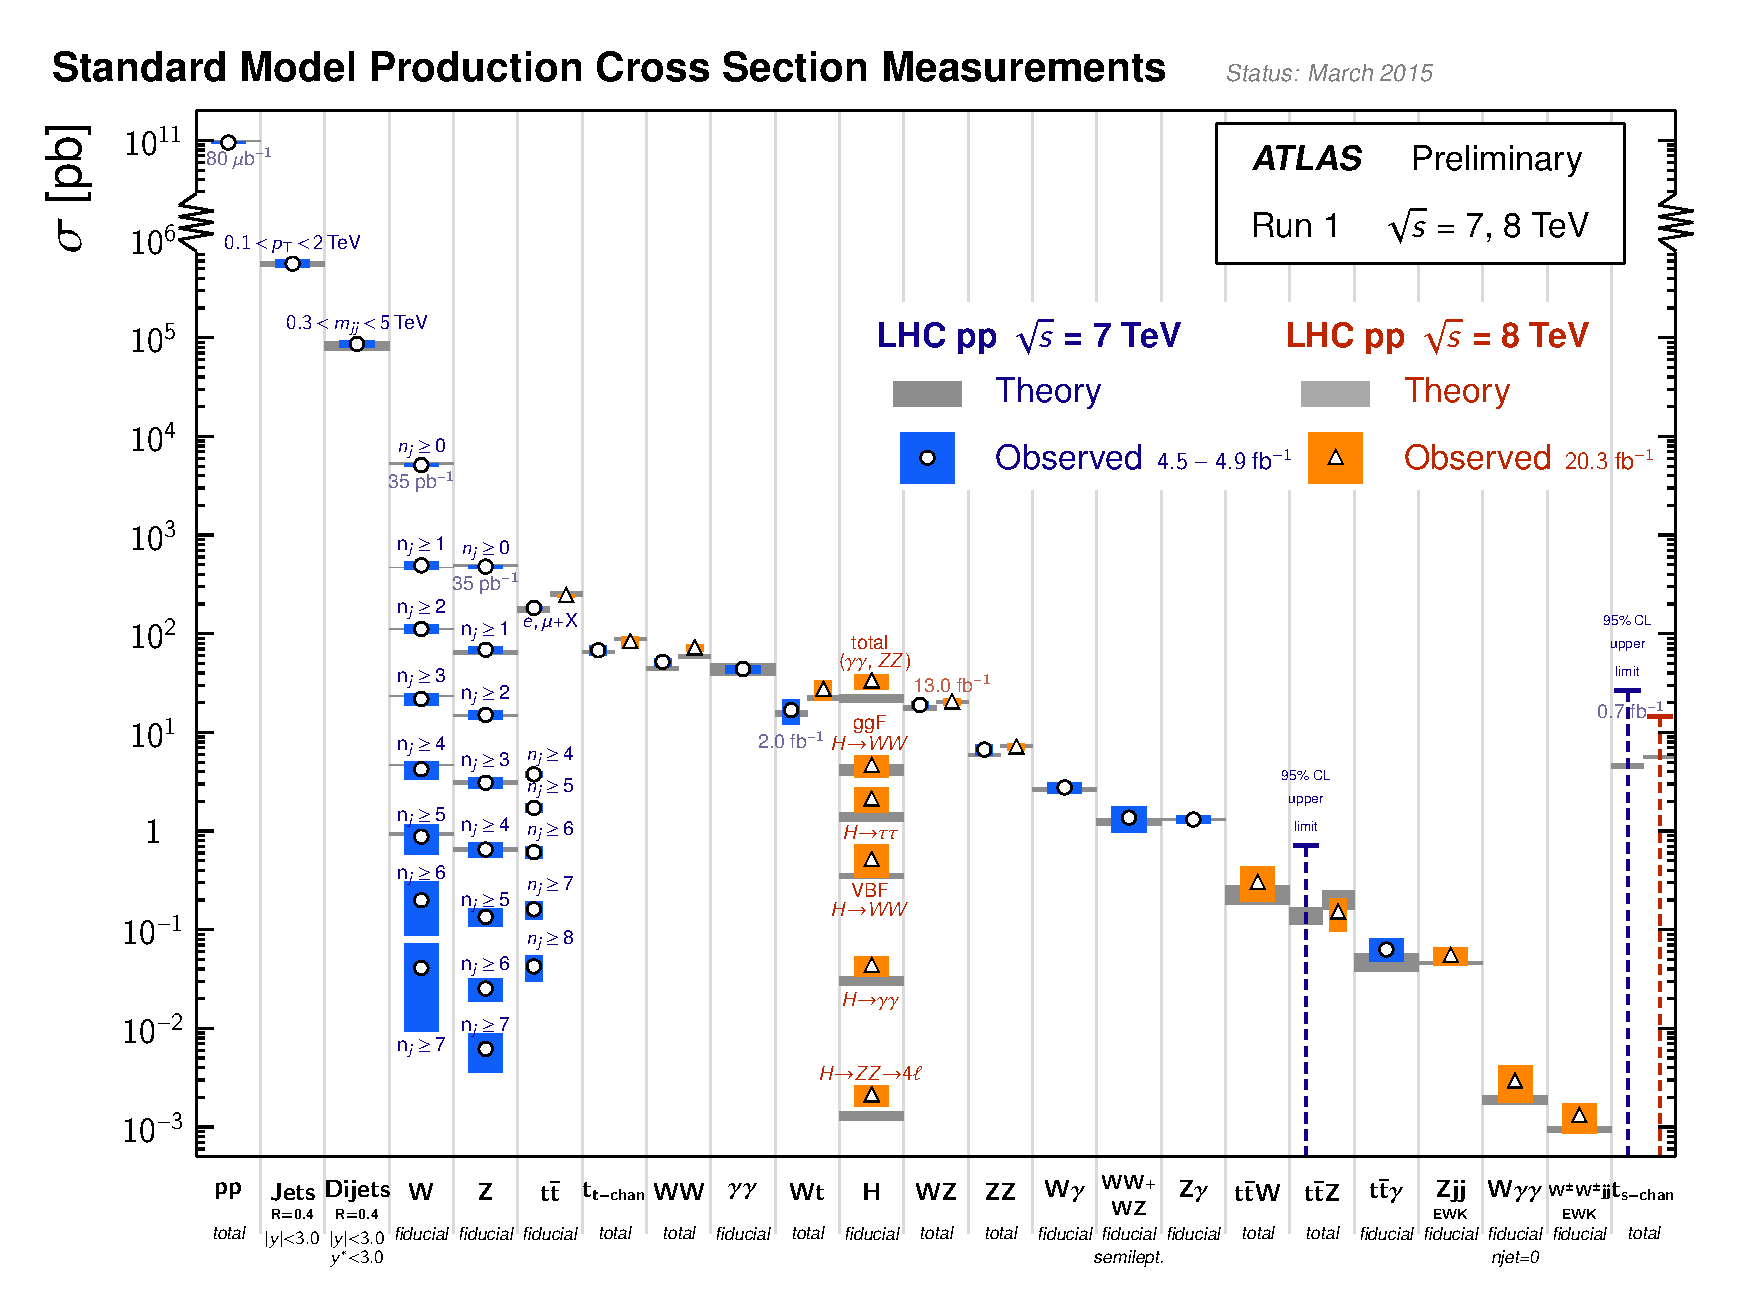
\includegraphics[width=0.7\textwidth]{summary2.pdf}
\label{fig:sm:summary}
\caption{Summary of SM cross-section measurements performed in ATLAS, showing the theoretical prediction and the observed value. The agreement across all the various channels is striking.}
\end{figure}

%%%%%%%%%%%%%%%% 

The theory consists of two main parts: the Glashow-Weinberg-Salam theory of electroweak interactions, which describes the electromagnetic and weak nuclear forces, and Quantum Chromodynamics, which describes the strong nuclear force. Together these form the symmetry group of the Standard Model, $SU(3)_C \otimes SU(2)_W \otimes U(1)_Y$. With the discovery of the Higgs Boson, the mechanism of symmetry breaking in the electroweak sector has been elucidated, and all the particles predicted by the model have been identified. While the SM is complete in this sense, there are still many questions which it does not address, and some of these will be discussed in Chapter~\ref{chapter:susy} and \ref{chapter:search}. At the same time, some predictions of the SM--- the rate of decay channels of the Higgs Boson, or the details of parton showering in QCD--- are still not fully understood, and one new measurement of such SM phenomena is presented in Chapter~\ref{chapter:color}.

The following chapter gives an overview of the SM and outline some of its most powerful successes. The approach will be very cursory, aiming to give a broad overview of the SM Lagrangian and how various parts of it function; detailed references can be found in \cite{schwartz,2006physics11219P}. 



\section{The Electroweak Force and Spontaneous Symmetry Breaking}

To start, we characterize the electroweak force, i.e. the $SU(2)_W \otimes U(1)_Y$ part of the SM. Note that the $U(1)_Y$ is the gauge group of \textit{hypercharge}, not the low-energy $U(1)$ associated with electromagnetism. Similarly, the particles associated with the $SU(2)_W$ are not the vector bosons $W$ and $Z$: instead, linear combinations of all these fields form the familiar mass eigenstates~\cite{Glashow:1961tr,Weinberg:1967tq,Salam:1968rm}. 

The Lagrangian of the electroweak sector (writing down all renormalizable and gauge-invariant terms), is:
%
\begin{equation}
\label{eqn:sm:electroweak_l}
\mL = - \frac{1}{4} (W_{\mu\nu}^a)^2 - \frac{1}{4} B_{\mu\nu}^2 + (D_\mu H)^\dagger (D_\mu H) + m^2 H^\dagger H - \lambda(H^\dagger H)^2,
\end{equation}
%,
where $W_\mu^a$ are the $SU(2)$ gauge bosons, $B_\mu$ is the hypercharge gauge boson (and $B_{\mu\nu} = \partial_\mu B_\nu - \partial_\nu B_\mu$), and $H$ is a complex doublet with hypercharge $1/2$, called the Higgs multiplet. The covariant derivative $D_\mu$ is defined as:
%
\begin{equation}
D_\mu H = \partial_\mu H - i g W_\mu^a \tau^a H - \frac{1}{2} i g' B_\mu H,
\end{equation}
%
with $g$ and $g'$ as the $SU(2)$ and $U(1)$ coupling constants, and $\tau^a$ as the standard $SU(2)$ generator. The last part of the Lagrangian, $V(H) = -m^2 |H|^2 +\lambda |H|^4$, is the \textit{Higgs potential}~\cite{Englert:1964et,Higgs:1964pj,Guralnik:1964eu}. A potential of this form has a minimum at $|\langle H \rangle| = \sqrt{\frac{2 m^2}{\lambda}}$, which induces a vacuum expectation value (vev) in the scalar field. This vev means that the ground state spontaneously breaks the symmetry of the potential. Written out in terms of the multiplet, and taken as real and in one direction only without loss of generality, this vev can be written as:
%
\begin{equation}
H = \exp \left( 2i \frac{\pi^a \tau^a}{v} \right) \colvec{2}{0}{\frac{v}{\sqrt{2}}+ \frac{h}{\sqrt{2}}}
\end{equation}
%
where $v = m / \sqrt{\lambda}$, and $h$ is a real scalar field. A simple gauage choice allows us to set $\pi = 0$, simplifying the phase of the vev. Plugging this into the covariant derivative term, and ignoring $h$ terms for now, we have:
%
\begin{equation}
|D_\mu H|^2 = g^2 \frac{v^2}{8} \left[ (W_\mu^1)^2 + (W_\mu^2)^2 + \left( \frac{g'}{g} B_\mu - W_\mu^3 \right) \right]
\end{equation}
%
These are the mass terms of the three massive gauge bosons (each proportional to $\frac{g^2 v^2}{8}$). To simplify these masses, we introduce $\tan(\theta_w) = \frac{g'}{g}$, which allows us to write:
%
\begin{align}
Z_\mu &\equiv \cos \theta_w W_\mu^3 - \sin \theta_w B_\mu\\
A_\mu &\equiv \sin \theta_w W_\mu^3 + \cos \theta_w B_\mu
\end{align}
%
and introduce a change of linear basis for the $W^{1,2}$ terms as $W_\mu^{\pm} \equiv \frac{1}{\sqrt{2}} (W_\mu^1 \mp i W_\mu^2)^2$. Plugging this into the original mass terms, we get:
%
\begin{align}
m_A &= 0\\
m_W &= \frac{v}{2} g\\
m_Z &= \frac{v}{2} \sqrt{g^2 +g'^2} = \frac{m_W}{\cos \theta_w}
\end{align}
%
These are the mass terms of the familiar photon, $W$, and $Z$ bosons. The original Lagrangian in Equation~\ref{eqn:sm:electroweak_l} contained only massless bosons: in fact, writing down masses directly would break the $SU(2)$ invariance of the Lagrangian. Instead, the breaking of the symmetry of the Higgs potential with the vev has given masses to the various linear combinations of the initially massless bosons. These mass terms originate as three out of the four original degrees of freedom of the complex Higgs doublet. 

Using these transformations on the rest of the original Lagrangian allows for the derivation of the kinetic terms of each boson, as well as the interactions (which are considerably more complicated now that we have broken the original electroweak symmetry). Returning now to the previously ignored $h$ term, we can collect its kinetic terms and couplings to get:
%
\begin{equation}
\mathcal{L}_\mathrm{Higgs} = - \frac{1}{2} h \left(\square + \frac{2\lambda}{v^2}\right) h + \mathrm{interactions}.
\end{equation}
%
These are the kinetic and (tree-level) mass terms of a new scalar particle, the Goldstone boson associated with the vev spontaneously breaking the electroweak symmetry, and the last degree of freedom of the original complex Higgs multiplet. This Higgs boson, discovered by the ATLAS and CMS collaborations on July 4, 2012, was the ``last piece'' of the Standard Model, and its discovery confirmed one of the final open questions of the SM~\cite{Aad:2012tfa,Chatrchyan:2012ufa}. That is not to say that there are no remaining puzzles, and indeed, Section~\ref{chapter:susy:problems} will address some that are directly related to the Higgs.

\section{Quantum Chromodynamics and Strong Interactions}

%define QCD lagrangian, discuss renormalization at high level, sign of beta function leading to asymptotic freedom
Next, we characterize the Quantum Chromodynamic (QCD) force, which is governed by the symmetry group $SU(3)_C$~\cite{Politzer:1973fx,Gross:1973ju,Gross:1973id}. The QCD Lagrangian, defined by writing down all renormalizable and gauage invariant terms, is defined as:
%
\begin{equation}
\mL_{\mathrm{QCD}} = \sum_f i \bar{\psi_f} D_\mu \gamma^\mu \psi_f - \frac{1}{4} G_{\mu\nu}^a G_{a}^{\mu\nu},
\end{equation}
%
where the covariant derivative is defined as:
%
\begin{equation}
D_\mu = \partial_\mu - i g_s G_\mu^a T^a
\end{equation}
%
The sum is over the $f$ families of the quarks, $\psi_f$, which will be described in more detail in Section~\ref{chapter:sm:matter}; $g_s$ is the strong coupling constant, $G_\mu^a$ are gluon fields, and $T^a$ are the generators of the $SU(3)$ group. $G_{\mu\nu}^a$, like the $B_{\mu\nu}$ terms from the electroweak interaction, is a field strength, defined as:
%
\begin{equation}
G_{\mu\nu}^a \equiv \partial_\mu G_\nu^a - g_s f^{abc}G_\mu^b G_\nu^c
\end{equation}
%
where $f^{abc}$ are the $SU(3)$ structure constants. The first term in the Lagrangian clearly provides the kinetic term for the quarks, and their interactions with gluons; the second term, when expanded, provides the kinetic term for gluons and their self-interactions, which include terms with both 3-gluon vertices and 4-gluon vertices. Note the Lagrangian has been written with the color index suppressed: the $\psi$ are in reality column vectors over $\alpha$, the color index, and the $G$ term is a matrix, with two color indices $\alpha, \beta$. This color charge of quarks and gluons, typically identified as red, blue, and green, gives rise to a number of interesting phenomena. %For example, the three quarks are essentially independent particles, explaining why decays of particles such as the $Z$-boson are more prevalent to quarks (as decays occur equally to all types, and the additional color factor means there are more types of quarks).

\subsection{Asymptotic Freedom}
\label{chapter:sm:qcd:freedom}
The quantization of the QCD Lagrangian (or really, any field theory) allows for so-called \textit{loop terms}, such as Figure~\ref{fig:sm:loop}, to appear in calculations. These loops, which appear as perturbative corrections for many processes, are formally infinite as the momentum in the loop is integrated over all possible momentums and grows without bound. The solution to these divergences is a technique referred to as \textit{renormalization}, which deforms the theory in such a way as to keep the solutions finite. Several renormalization schemes--- which all give the same results--- exist, and they can all be thought of as setting some scale which cuts off the infinite integrals in the loops, or which absorb the ``bad,'' un-physical, infinite part of an integral and leave a physical result. The loops then become finite corrections to various properties of the theory--- masses, coupling constants, etc.--- accurate to some order of the perturbative expansion~\cite{schwartz}.

%%%%%%%%%%%%%%%%

\begin{figure}
\centering
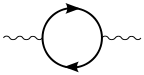
\includegraphics[width=0.25\textwidth]{loop.png}
\label{fig:sm:loop}
\caption{An example of a loop, whose contribution to a matrix element is formally infinite, in a QFT calculation.}
\end{figure}

%%%%%%%%%%%%%%%% 

One particularly interesting set of corrections is for the coupling constant, $g_s$ for the strong force\footnote{$g$ and $g'$ for the electroweak force also receive such a correction, but for reasons that will be explained, this correction is not as important for the electroweak force.} The correction to the coupling constant is parameterized by the $\beta$-function, which is used as a part of the \textit{renormalization group equation} to characterize the evolution of the coupling as a function of the $\mu/\Lambda$, or the energy scale over some reference scale of the theory. A positive value of the $\beta$-function implies that the strength of the coupling grows with energy--- this is the direction of the evolution of the electroweak couplings, for instance\footnote{In particular, the $\beta$-function is the coefficient of a $\ln{\mu/\Lambda}$ term in the RGE equation which determines the strength of the coupling constant $g$. So the sign of the $\beta$-function determines whether the RGE is a growing or shrinking exponential, to first order.}. The $\beta$-function for QCD, on the other hand, is:
%
\begin{equation}
\beta(\alpha_s) = - \frac{\alpha_s^2}{2\pi} \left(\frac{11}{3} n_\mathrm{colors} - \frac{4}{3}n_\mathrm{flavors}\right)
\end{equation} 
%
where $\alpha_s = g_s^2 / 4\pi$. The terms here arise from a particularly long calculation (see \cite{schwartz}), but can be understood to arise from gluonic self-interactions for the first term and $q-\bar{q}$ loops for the second term. Since in the SM QCD $n_\mathrm{colors} = 3$ and $n_\mathrm{flavors} = 3$, this combined quantity is negative: the strength of QCD shrinks as the energy scale increases. This phenomena is referred to as \textit{asymptotic freedom}: as the energy scale $\mu$ approaches infinity, the strength of the force drops to zero. Conversely, at low energies, the coupling constant approaches infinity, meaning that the perturbative expansion used to derive this breaks down, and a new approach must be taken~\cite{Gross:1973ju,Gross:1973id}.

\subsection{Confinement}
\label{chapter:sm:qcd:confinement}

The non-perturbative evolution of $g_s$ at low $\mu$ suggests that a transition occurs in the theory: this is the process of \textit{color confinement}~\cite{Wilson:1974sk}. Confinement means that objects which are charged under the strong force--- quarks and gluons--- will form bound states with neutral color, so that color is never observed directly. Free quarks and gluons, produced in collisions or decays of other particles, will use some of their energy to create partners to form neutral combinations. This process is also referred to as \textit{hadronization}, in that it is the transition of the partons of QCD into the stable (or semi-stable) hadrons (either mesons, composed of two quarks, or baryons, composed of three quarks) which are observable in experiment. 

This process has an incredible impact on the experimental accessibility of strongly interacting particles: in particular, it means that such particles are never directly observable, but will only ever be seen through the shadow of the hadrons they created. Combined with the \textit{parton shower}--- the radiative process of gluons splitting to quarks and each of these emitting gluon radiation--- this creates the observed phenomena of \textit{jets}: the collimated sprays of measurable particles which correspond to some initial colored particle. Chapter~\ref{chapter:jets-and-substructure} discusses many of the theoretical issues in dealing with jets, and recent advances in the theoretical understanding of these objects; Chapter~\ref{chapter:jet-reconstruction} addresses the experimental issues associated with measuring and reconstructing them.


Finally, it should be noted that the details of confinement are still very mysterious: there is no known mechanism for the transition to this state, and no rigorous proof even that the dynamics of QCD at low $\mu$~should generate bound states. Regardless, there is a great deal of experimental evidence which confirms the evolution of $\alpha_s$ with energy, and the existence of jets and lack-of-observation of colored particles strongly suggest that confinement is very much real. As with any process in physics, though, detailed understanding becomes much more difficult when a process becomes non-perturbative.

\subsection{Parton Distribution Functions}

At a hadron collider such as the LHC, confinement plays an interesting role in determining not only the outgoing particles--- in the form of jets--- but also the incoming particles, through a process described by \textit{parton distribution functions} (PDFs)~\cite{PhysRevD.30.49}. The protons which the LHC accelerates are not in fact fundamental objects: they are composed of two up quarks one one down quark (these will be defined in more detail in Section~\ref{chapter:sm:matter}), and the gluons which hold them together. This means collisions at the LHC are not really between protons, but between the partons \textit{inside} the protons. Thus, calculations of cross-sections at hadron colliders are not done at a particular energy, or even with specific parton inputs, but instead must be averaged over a distribution of possible input particles and energies those particles might have.

To make matters even more interesting, the deep structure of the proton is much more complicated than a simple view of $uud$ would suggest. The internal gluons holding the hadron together can split into virtual quark/anti-quark pairs before reforming to gluons: these virtual quarks, referred to as \textit{sea} partons (as opposed to the \textit{valence} partons $uud$), as well as the gluons inside the proton, can also participate in collisions.

Thankfully, the situation is not completely hopeless: the QCD factorization theorem states that the cross-section of a hard-scattering (i.e., the $2\ra2$ or $2\ra n$ prcoess describing the actual collision) can be factorized from the non-perturbative structure of the hadrons causing the collision. The probability of a particular parton from the proton interacting at some momentum-scale $Q^2$ with some energy fraction $x$ from the proton is parameterized by the PDF's previously mentioned. An example is shown in Figure~\ref{fig:sm:pdf}: at low energy, or low $Q^2$, the $u$ and $d$ quark (as well as the gluon) are dominant, but at higher $Q^2$ it is possible for even sea $c$ and $b$ quarks to participate in interactions. Many different parameterizations of PDFs are available, each using a variety of measurements and theories to constrain the provided functions~\cite{Whalley:2005nh,PDF-MRST,PDF-CTEQ,Ball:2008by,Ball:2010de,cteq6l1,Martin:2009iq,Botje:2011sn}.



%%%%%%%%%%%%%%%%

\begin{figure}
\centering
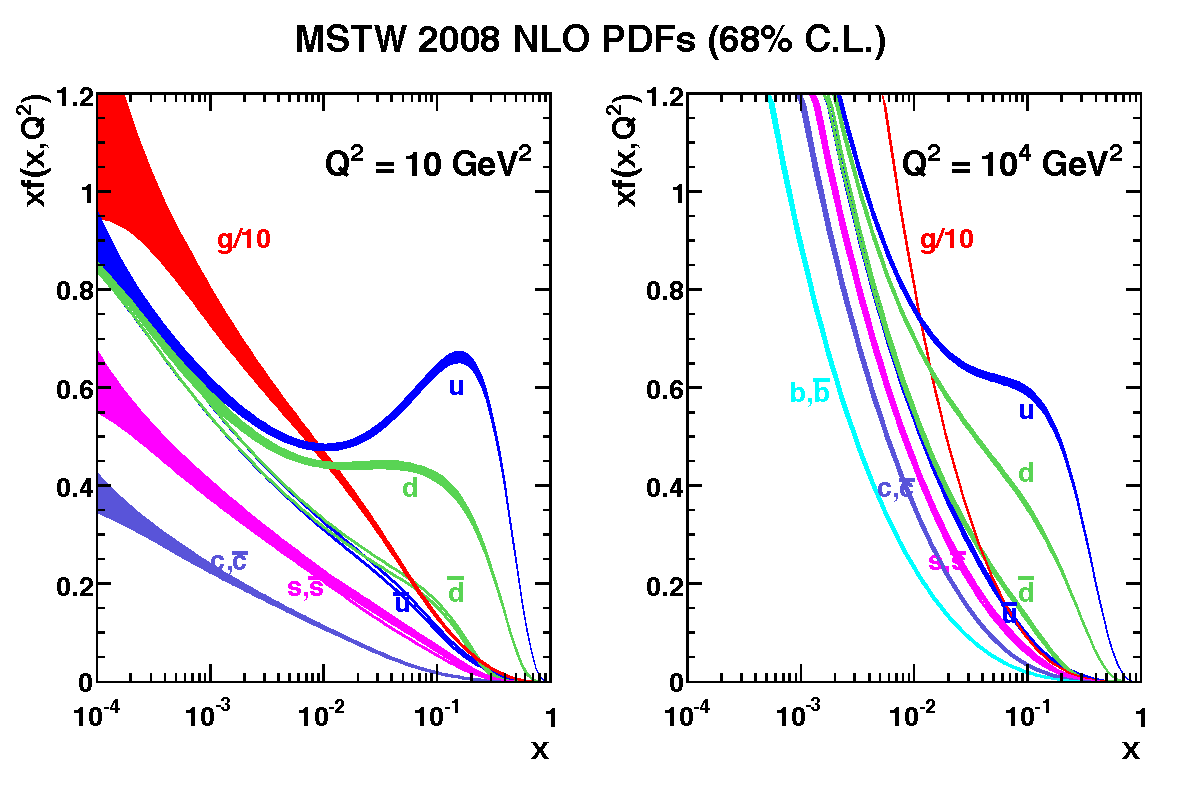
\includegraphics[width=0.7\textwidth]{mstw2008nlo68cl_allpdfs}
\label{fig:sm:pdf}
\caption{An example of a PDF set--- in this case the MSTW2008NLO--- which characterizes the probability of a particular particle inside the proton interacting, as a function of the momentum-fraction $x$ and the momentum scale $Q^2$~\cite{Martin:2009iq}.}
\end{figure}

%%%%%%%%%%%%%%%% 

% The process of confinement, and its relationship with asymptotic freedom, can be understood better in certain limits. For example, consider a pair of quarks in a bound state. At very high $\mu$-- that is, very small distance scales-- the particles are free to move without restriction, as the ``rubber band'' that is holding them together has not been stretched. As we transition to lower e


\section{Matter}
\label{chapter:sm:matter}

The gauge bosons of the fundamental symmetry groups of the SM are commonly referred to as force-carriers, as they mediate the interactions of their respective sectors. Another class of particles, called \textit{matter}, is not responsible for the mediation of forces. Unlike the force-carriers, which are all which are all bosons and have integer spin, matter particles are all fermions and have half-integer spin. Matter in the SM is composed of 3 generations each of the previously mentioned quarks, and another family of fermions referred to as leptons which do not carry color charge. Each generation consists of a pair of related particles; each generation is identical to the other generations except for the masses of the particles. Each fermion also has an anti-particle partner, which is alike in all ways except for having the opposite charges~\cite{schwartz}.

\subsection{Quarks}

Quarks, as already described, are the constituent particles of protons, neutrons, and the remainder of the hadron zoo. They are charged under the $SU(3)_C$ of the strong force, so they interact with the strong force via gluons; they are also charged under $SU(2)_W \otimes U(1)_Y$, so they also interact with the $W$, $Z$, and $\gamma$ of the electroweak force. The various types of quarks, paired into generation columns, are:
%
\begin{equation}
\label{eqn:quarks}
\colvec{2}{u}{d},  \colvec{2}{c}{s},  \colvec{2}{t}{b}
\end{equation}
%
and are commonly referred to as the up, down, charm, strange, top, and bottom flavors. The top row is commonly referred to as ``up''-type, and all have electric charge of $+2/3$; the bottom row is referred to as ``down''-type and has electric charge of $-1/3$. The lightest generation is listed on the left, and the heaviest on the right. The $u$ are $d$ nearly degenerate in mass, with masses of $2.3$ and $4.8$ MeV respectively, while the $s$ is not much heavier at $95$ MeV: for the purposes of many applications in high-energy experiments, these are all effectively massless. The remaining quarks, however, are much heavier: the $c$ has a mass of $1.3$ GeV, and the $b$ has $4.2$ GeV. The top is even more massive, at $173$ GeV: approximately the same mass as an atom of gold. This mass is so high that the top quark, unlike the others, decays before it has the time to hadronize\footnote{Typically decay lifetimes are inversely proportional to masses, so the heaviest particles will decay quickest.}, and no top quark bound states exist. These masses are free parameters of the theory, and arise via a mechanism described in Section~\ref{chapter:sm:matter:masses}--- while there is no expectation that they be identical, there is also no explanation for them having such different properties~\cite{schwartz}.

\subsection{Leptons}

Leptons are the second category of matter: they all interact via the weak force, and none are charged under the strong force~\cite{schwartz,Weinberg:1967tq}. Once again, they have three generations organized into pairs:
%
\begin{equation}
\label{eqn:leptons}
\colvec{2}{\nu_e}{e},  \colvec{2}{\nu_\mu}{\mu},  \colvec{2}{\nu_\tau}{\tau}
\end{equation}
%
The bottom row, referred to as the ``charged leptons'', all have charge $-1$, and have mass in increasing order of the generation. They are called the electron, muon, and tau, respectively. The electron is completely stable, while the muon has a lifetime on the order of $10^{-6}$~s, and therefore is stable as far as high-energy experiments are concerned. The $\tau$ has a much shorter lifetime, and can decay into the other leptons or to hadrons, making the identification of $\tau$'s much more challenging at the LHC than the other leptons. For this reason, ``leptonic'' analyses at the LHC often refer to analyses involving the first two generations only.

The top row of Equation~\ref{eqn:leptons} is referred to as neutrinos: these particles, as the name suggests, are electrically neutral and therefore do not interact with the photon. Almost all particle detection mechanisms at the LHC (see Chapter~\ref{chapter:detector}) rely on the particle interacting with the detector electromagnetically, and so for this reason, neutrinos are not directly observed in collision events. Instead, their presence is inferred from mis-balances in momentum and energy conservation (in the transverse plane). Neutrinos are also effectively massless: while observations over the past 20 years~\cite{Ahmad:2001an} have confirmed that they do have masses, they are so vanishingly small that they have little experimental consequence at the LHC.

\subsection{Interactions}

The matter particles described now are all written in the Dirac representation, which combines $L$ and $R$ chiralities into a single spinor object.  Above the electroweak breaking scale, it is also possible to write them as $SU(2)$ doublet pairs (paired following the column structure of Equations~\ref{eqn:quarks} and \ref{eqn:leptons}): these are referred to as $Q^i$ and $L^i$ respectively, and contain the left-handed fields only. The right handed fields are uncharged under the weak interaction, and therefore form the $SU(2)$ singlets $e_R^i$, $\nu_R^i$, $u_R^i$ and $d_R^i$\footnote{Technically, the right-handed $\nu_R^i$ have not been observed, as only the neutrinos which interact via the weak force have been measured.}

Since the $Q$ and $L$ doublets interact via the weak force, interaction terms for them look like:
%
\begin{equation}
\label{eqn:weak-interactions}
\mL_\mathrm{interactions} = i \bar{L}_i (\gamma^\mu \partial_\mu - i g \gamma^\mu W_\mu^a \tau^a - i' Y_L \gamma^\mu B_\mu) L_i
\end{equation}
%
with a similar term for $Q$; the singlets interact only with the hypercharge boson, $B$. The off-diagonal terms of the $W\tau$ term (which contain the $W_1$ and $W_2$ terms) couple together the top and bottom rows of the $SU(2)$ doublets. Once everything is re-written in the mass eigenstates once the electroweak symmetry is broken, this means that the $W^\pm$ bosons (the linear combinations of $W_1$ and $W_2$) exchange an up-type quark for a down-type quark or vice versa (and likewise exchange charged-leptons for neutrinos). The structure of the weak interaction thus has very interesting consequences for how matter interacts with it~\cite{Glashow:1961tr,Weinberg:1967tq,Salam:1968rm}.

\subsection{Masses}
\label{chapter:sm:matter:masses}

Just as for the gauge bosons, mass terms for fermions are problematic: a Dirac mass term like $m \bar{\psi} \psi = m\bar{\psi}_L \psi_R + m \bar{\psi}_L \psi_R$ is not invariant under the $SU(2)$ group, as the $SU(2)$ transformation affects only the left-handed component. The solution is to couple the the matter terms to the Higgs boson via a Yukawa coupling:
%
\begin{equation}
\mL_\mathrm{Yukawa} = - y \bar{Q} H d_R + h.c.
\end{equation}
%
The $Q$ and $H$ transform with an opposite phase under an $SU(2)$ transformation, and thus maintain gauge invariance. After symmetry breaking this generates a mass term of the form $-m_d(\bar{d}_L d_R + \bar{d}_R d_L)$--- recall that we choose $\colvec{2}{0}{v}$ as the direction of the Higgs field, so only the down-type quarks gets a mass from this--- where $m_d = \frac{y}{\sqrt{2}}v$. The up-type quarks get a mass from a similar term, using $\bar{Q}\sigma_2 H^*$ to rotate the vev into the up-type sector while preserving gauge invariance. Thus, mass originates not as a fundamental property of a particle, but from the interaction of the particle with the Higgs field. Different masses are possible as a consequence of different Yukawa couplings for each particle~\cite{schwartz}.

In order to provide for the masses of multiple generations of quarks, a more complicated Yukawa structure using matrices (indexing the flavor via $i,j$) is required:
%
\begin{equation}
\label{eqn:yukawa_masses}
\mL_\mathrm{mass} = -Y_{ij}^d \bar{Q}^i H d_R^j - i Y_{ij}^d \sigma_2 H^* u_R^j + h.c.
\end{equation}
%
After symmetry breaking, this reduces to:
%
\begin{equation}
\mL_\mathrm{mass} = - \frac{v}{\sqrt{2}} (\bar{d}_L Y_d d_R + \bar{u}_L Y_u uR) + h.c.
\end{equation}
%
These Yukawa matrices are arbitrary, and are in general not diagonal: this means that once we diagonalize the matrix to the mass eigenbasis:
%
\begin{equation}
\mL_\mathrm{mass} = - m_j^d \bar{d}^j_L d^j_R - m_j^u \bar{u}_L^j u^j_R + h.c.,
\end{equation}
%
this is \textit{not} the same as the original $SU(2)$ interaction basis written down in Equation~\ref{eqn:quarks}. In fact, if we transform the interactions of Equation~\ref{eqn:weak-interactions} with the diagonalization matrix used to change these bases, we will see that most terms transform cleanly, but terms which mix $u_L$ and $d_L$ will not remain diagonal in the flavor-basis. The particles we are familiar with exist in the mass eigenstate, and so it is most common to adopt that basis and introduce off-diagonal terms into the interactions. This means, for example, that while the $W$ usually decays to $ud$ or $cs$, it can also decay to $us$ or $cd$. The exact level of non-diagonalization is parameterized by the \textit{CKM matrix}~\cite{PhysRevLett.10.531,Kobayashi01021973}: most terms are very close to on-diagonal, but the rate of decays for the $W$ to $us$ and $cd$ are approximately $4\%$.

Note that because the charged-leptons correspond to the ``down''-type, and the neutrinos are massless\footnote{At least, their masses seem to most likely be acquired via a different mechanism, not described here.}, the second term of Equation~\ref{eqn:yukawa_masses} is not necessary in the lepton-mass sector. Therefore there is no problem in diagonalizing the mass-basis and interaction-basis simultaneously, there is no CKM matrix for the lepton sector~\cite{schwartz}.

%define matter fields, how they interact with ew, some lagrangian details, section 29.3 from S

\section{Summary}

The particle content of the Standard Model is summarized in Figure~\ref{fig:sm:summary}: the Higgs boson sits at the heart of the theory, the 4 gauge bosons interact with matter and transmit the forces, and the 12 matter particles form the atoms which we are all composed of. It is a remarkably concise theory: simply the statement of three generations of matter, the $SU(3)\times SU(2)\times U(1)$ gauge symmetry, the non-trivial minimum of the Higgs-potential, and Lorentz invariance gets us remarkably far in uniquely determining the shape of the theory. It took decades of theoretical insight and experimental work to create such a powerful description of the Universe, but the resilience of SM predictions to even very high energies proves the soundness of the underlying theory. 

%%%%%%%%%%%%%%%%

\begin{figure}
\centering
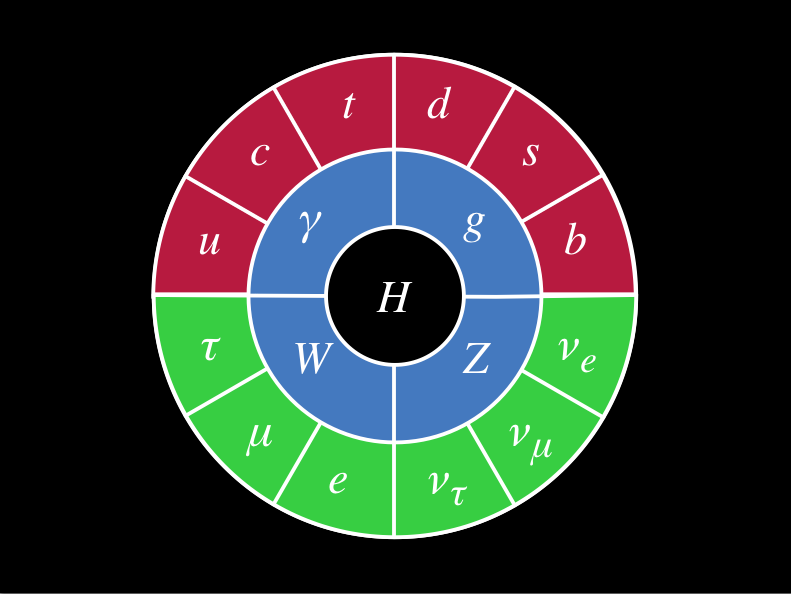
\includegraphics[width=0.8\textwidth]{Particle-Fever-Standard-Model-Graphic.png}
\label{fig:sm:summary}
\caption{Summary of the particle content of the Standard Model. Graphic courtesy of Particle Fever and Quantum Diaries.}
\end{figure}

%%%%%%%%%%%%%%%% 



\chapter{Jets and Substructure}
\label{chapter:jets-and-substructure}
\section{The Goal of Jets, and Jet Algorithms}
\section{Jet Substructure: Going Deeper}
\section{Calculations with Jets}


\chapter{Supersymmetry, $R$-Parity, and Naturalness}
%!TEX root = ../swiatlow_thesis.tex
\label{chapter:susy}

\section{The Problem of the Standard Model}
\label{chapter:susy:problems}

It is somewhat incongruous to say that the SM has problems after describing the degree of its success in Chapter~\ref{chapter:sm}, but there are clear tensions in the model which point to signs of potential new extensions. The following chapter describe some of these shortcomings, and introduces an extension called \textit{supersymmetry} that alleviates some of these issues\cite{Miyazawa:1966,Ramond:1971gb,Golfand:1971iw,Neveu:1971rx,Neveu:1971iv,Gervais:1971ji,Volkov:1973ix,Wess:1973kz,Wess:1974tw}. The experimental consequences of supersymmetry are then discussed, and the landscape of searches at particle colliders is evaluated.

\subsection{The Pursuit of Beauty, or Naturalness}
\label{chapter:susy:problems:naturalness}
The process of developing a fundamental theory of nature is intended to be simplifying: for example, the development of the parton model and QCD simplified the eight-fold way and the complicated sea of hadrons  that came before it~\cite{Politzer:1973fx,Gross:1973ju,Gross:1973id}. The core of this simplification was the realization of a symmetry--- the $SU(3)$ of color--- which reduced a complicated system to a more simple one. There is an element to this that a physicist might call beautiful: the realization of an underlying simple pattern which explains something complicated. In that sense, there should be very few accidents in a theory: there should be a \textit{reason} for things to be the way they are. For example, there are no accidental, or ad-hoc terms in a Lagrangian: we include all relevant terms allowed by the symmetry groups, and derive the consequences. The symmetry groups are the reason that the Lagrangians look the way they do \cite{schwartz}.

In this same sense, constants in the theory can be arbitrary, but requiring them to be \textit{arbitrarily precise} is something of an aesthetic problem: the theory should not care if the mass of the up or down quark were different by $50\%$, for example. However, there is exactly one such finely tuned mass in the Standard Model: $m_h$, the mass of the Higgs boson. 

As discussed in Section~\ref{chapter:sm:qcd:freedom}, higher-order terms caused by loop diagrams induce corrections to parameters, such as masses and coupling constants, through the process of renormalization. The Higgs boson's mass is not immune, and since the Higgs couples to all particles (except gluons) via either gauge coupling terms or the Yukawa couplings to matter, all of these particles create loops which correct the Higgs mass. Because it has the largest coupling, the loop involving the top quark--- pictured in Figure~\ref{fig:susy:higgs-loop}---  has the largest contribution out of all these terms~\cite{Martin1997}. The correction goes as:
%
\begin{equation}
\Delta m_H^2 \approx - \frac{|y_T|^2}{8\pi^2}\Lambda_\mathrm{UV}^2 + \ldots
\end{equation}
%
where $y_T$ is the top Yukawa coupling, and $\Lambda_\mathrm{UV}$ is the UV cutoff of the theory~\cite{Martin1997}. This correction grows quadratically with the cut-off scale: if the SM is the only theory of nature up to the Planck scale (where quantum gravity takes effect, thereby signficantly changing the appropriate physical description), then the correction is proportional to $M_\mathrm{Planck}^2$. The observed Higgs boson has a mass of 125 GeV~\cite{CombinedHiggs}, which is quite far from $M_\mathrm{Planck} = 1.22\times 10^{19}$~GeV: the only way to reconcile the measurement with the observation, is to set $m_0$, the bare Higgs mass before corrections, to a \textit{precise} value such that $m_0$ and $\Delta m_H^2$ cancel perfectly to 125 GeV. Thus, the SM requires the bare mass to be  defined to 1 part in $10^{19}$, a value so precisely specified that it seems unlikely to have arisen by chance. 

%%%%%%%%%%%%%%%%

\begin{figure}
\centering
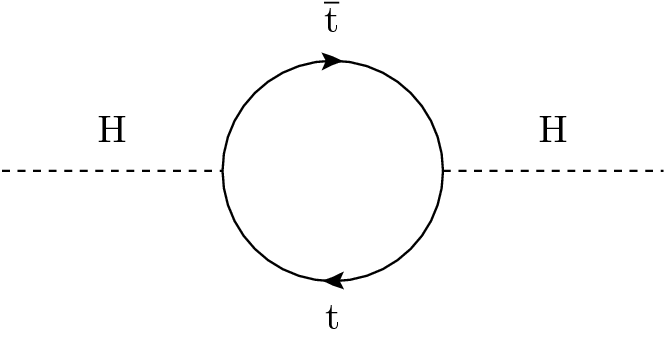
\includegraphics[width=0.7\textwidth]{higgs-loop.png}
\label{fig:susy:higgs-loop}
\caption{An example of a loop diagram which renormalizes the Higgs mass. Courtesy of PyFeyn.}
\end{figure}

%%%%%%%%%%%%%%%%  

Thus, the mass of the Higgs boson is not like that of other constants in the theory. Particles such as quarks and leptons do not receive quantum corrections to their masses, so there is no expectation for their masses; moreover, the observed mass of the Higgs is substantially outside of the expected range (around the Planck scale).  The SM's solution to this issue--- a precise cancelling of terms--- has an aesthetic penalty: there is no \textit{reason} for this cancellation in the SM, only blind luck. Physicists say that this kind of solution lacks \textit{naturalness}: there is no underlying symmetry or simplification to explain it, and only a very particular number.



\subsection{Unification}

Another aesthetic criticism of the SM lies in its separation of forces. The electroweak model is seen as particularly elegant because the electroweak symmetry, though broken at low energies by the Higgs mechanism, provides a unifying structure to two initially disparate forces (electomagnetism and the weak force). One natural question is whether some higher symmetry group unifies all the SM forces, and not just the electroweak. Figure~\ref{fig:susy:couplings_sm} shows the strength of the coupling constants in the SM as a function of the energy scale $\mu$: while they nearly intersect--- implying a potential for unification--- they just barely miss~\cite{susypheno}.


%%%%%%%%%%%%%%%%

\begin{figure}
\centering
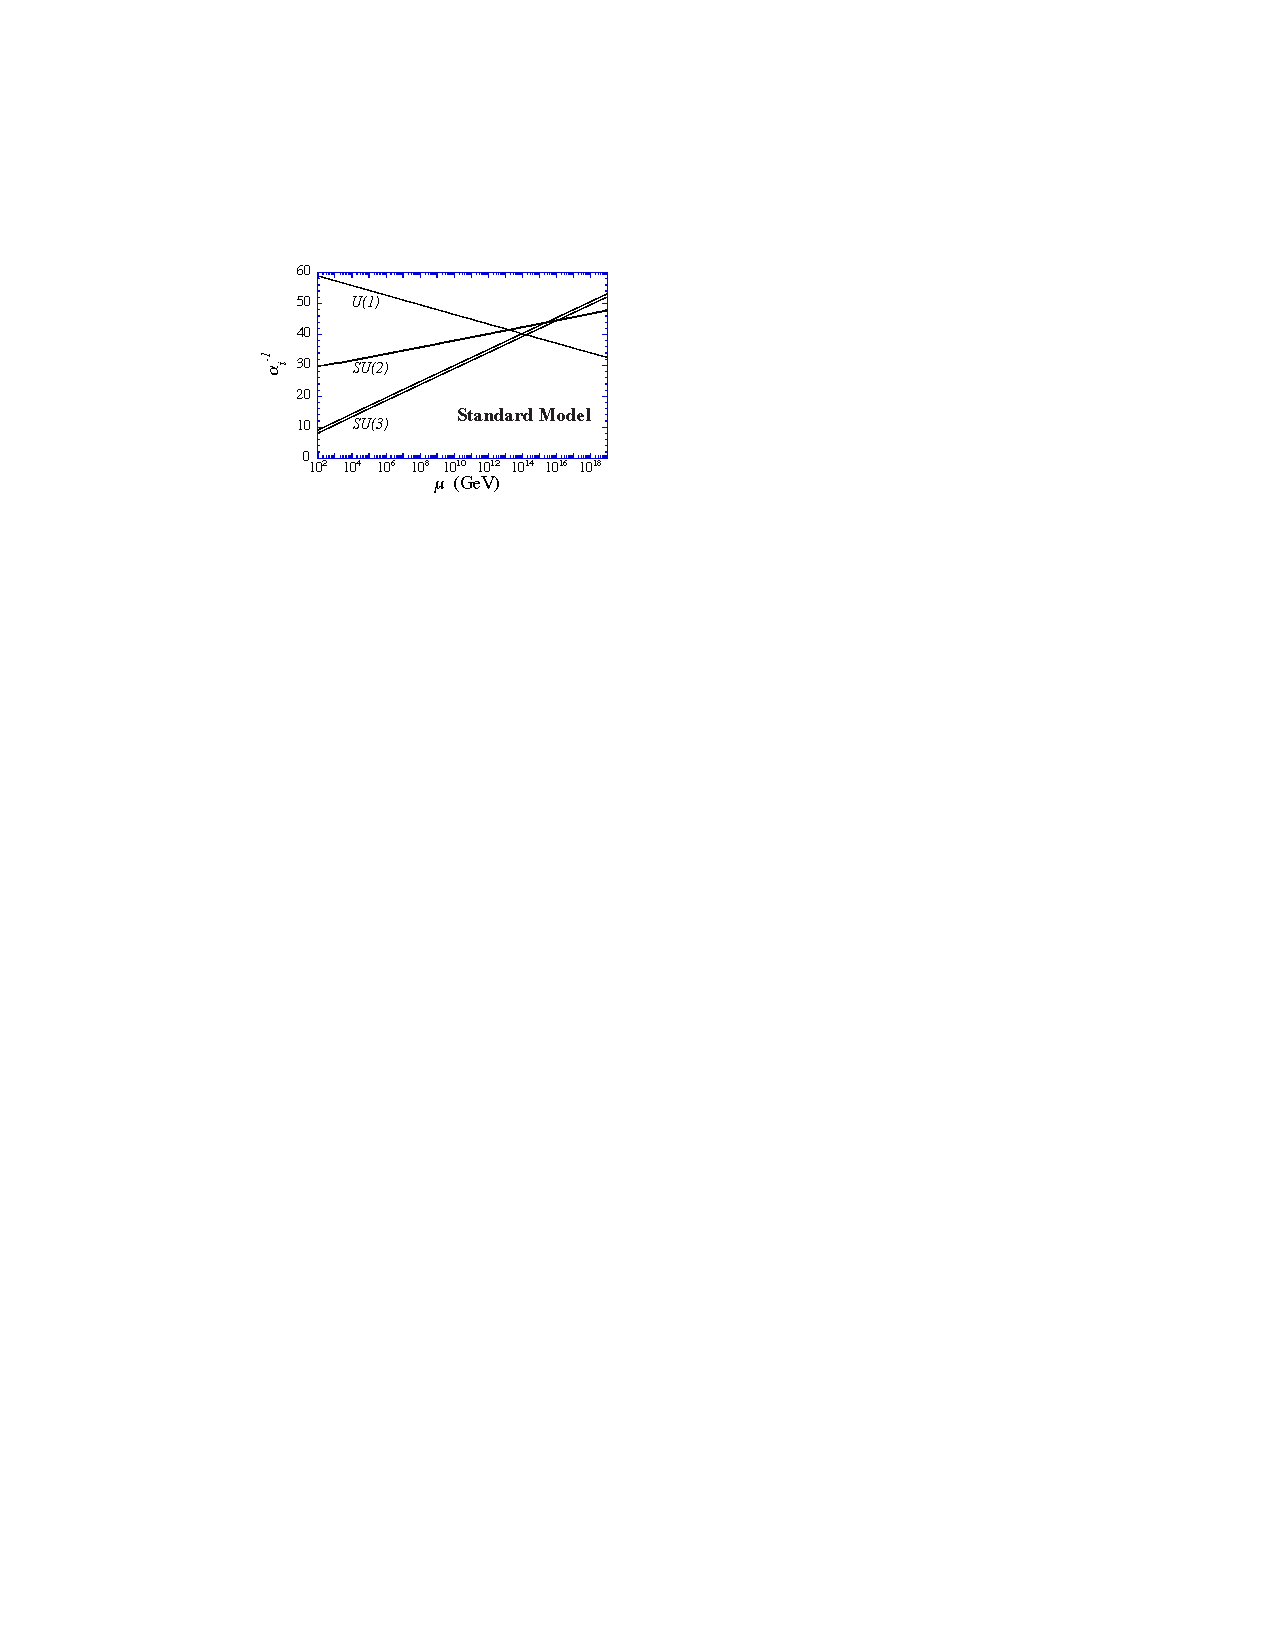
\includegraphics[width=0.7\textwidth]{couplings_sm.pdf}
\label{fig:susy:couplings_sm}
\caption{The evolution of the strength of the coupling constants of the three symmetry groups of the SM. While they come close to unifying, they never cross the same point. Figure from \cite{susypheno}.}
\end{figure}

%%%%%%%%%%%%%%%%  

While unification is certainly not \textit{required}, it seems like a shame that such an opportunity would be missed. Moreover, such a unification could explain the unexplained relationships in charge quantization between quarks and leptons~\cite{SUSYUnification}. Replacing two distinct forces with one overarching theory governed by one simple symmetry group would be a substantial simplification of the underlying model.

\subsection{Dark Matter}


One final motivation for the existence of physics beyond the SM is based on firm experimental ground: this is the presence of dark matter in the universe~\cite{Jungman}. Dark matter refers to the presence of matter that is inferred from observations of gravitational effects in the galaxy and beyond: these measurements indicate that there must be some source of mass, making up approximately 85\% of the mass of the universe, which does not emit light. Figure~\ref{fig:susy:bullet} shows one of the strongest observational pieces of evidence: the Bullet Cluster~\cite{Tucker:1998tp,Markevitch:2003at}. Two clusters of galaxies are passing through each other in this figure:; the blue area indicates regions with a large number of stars, while the purple area indicates areas with a large concentration gas which slowed down due to the collisions of the clusters. This gas contains most of the visible matter in the clusters, but gravitational lensing measurements (which study how light coming from behind the clusters bends) indicate that most of the mass occurs with the stars instead. This implies that another type of matter also passed through the collision along with the stars, and is hypothesized to be Dark Matter. Many other observations, such as the distributions of rotational speeds in sprial galaxies~\cite{Rubin}, the simulations of large scale structures in the universe~\cite{Springel:2005nw}, and measurements of the cosmic microwave background radiation~\cite{Ade:2015xua}, yield a consistent story of a significant amount of unaccountable matter.


%%%%%%%%%%%%%%%%

\begin{figure}
\centering
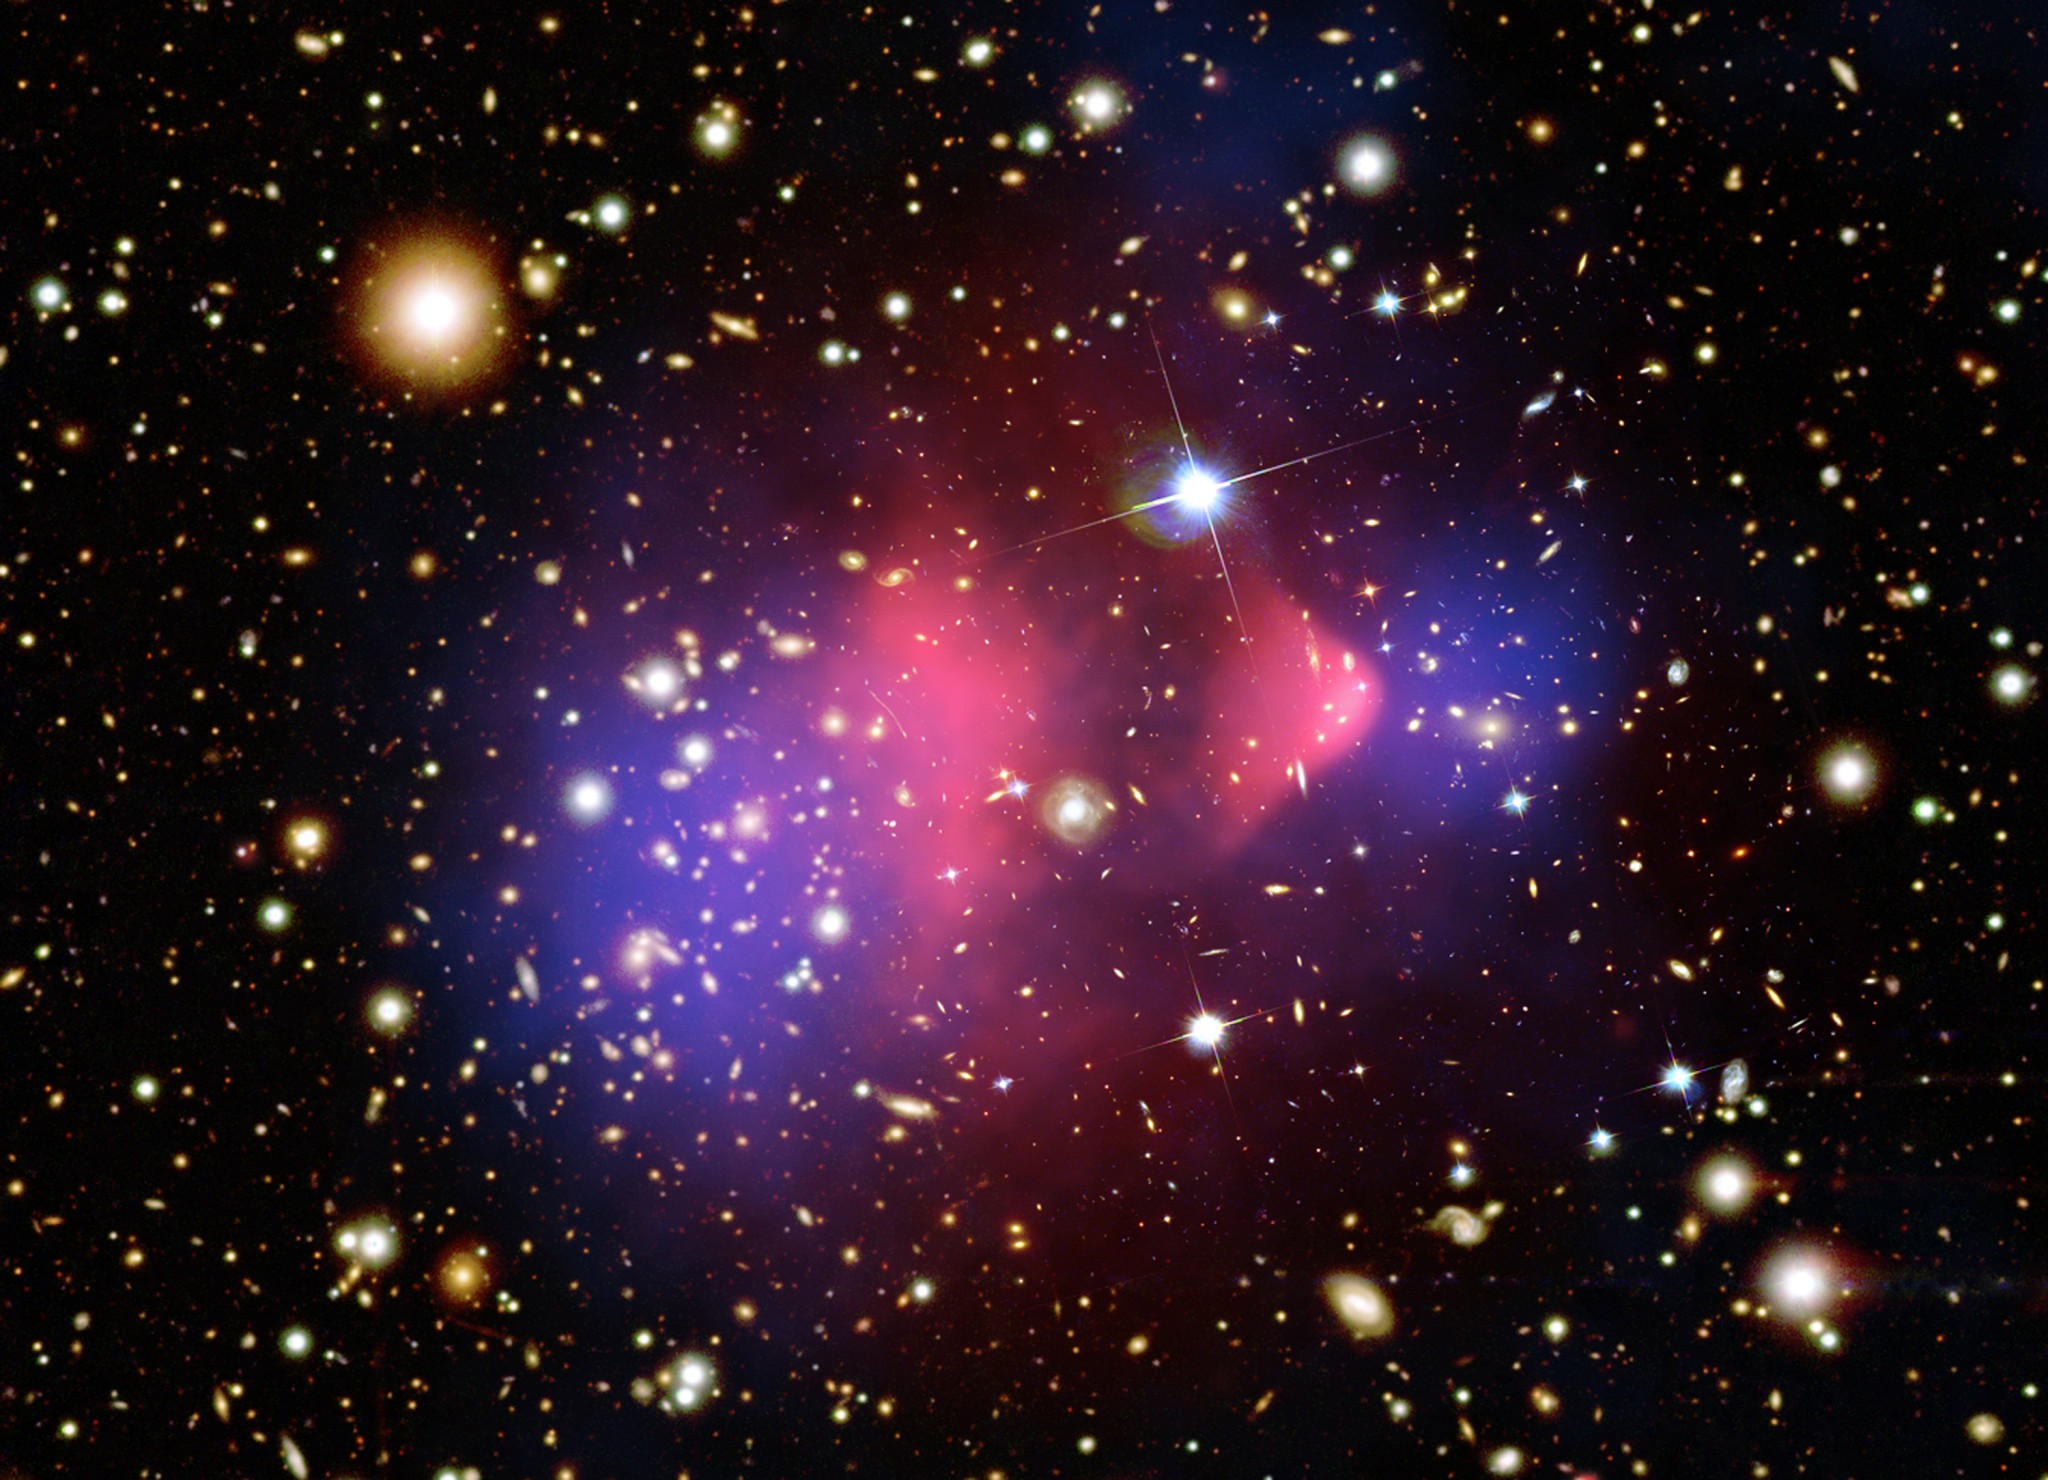
\includegraphics[width=0.7\textwidth]{bullet}
\label{fig:susy:bullet}
\caption{A false-color image of the Bullet Cluster, two colliding clusters of galaxies. The purple coloring indicates the stronger presence of gravitionally inferred mass, while the blue coloring indicates the stronger presence of electromagnetically observed mass.}
\end{figure}

%%%%%%%%%%%%%%%%  

Since dark matter is interacting gravitionally, and all other matter we are familiar with has come in the form of particles, it is natural to ask what particle dark matter possibly could be. There is one matter particle in the SM which interacts weakly and is therefore a potential candidate: these are the neutrinos, $\nu$. Unfortunately, their vanishingly small mass means that they would not be very strongly gravitionally interacting either, while many observations (such as the mass of galaxies) suggest that dark matter can ``clump'' together. This means that there are no candidates in the SM for dark matter, and we must look beyond the standard model to understand the nature of dark matter~\cite{Jungman}.


\section{Supersymmetry: The Solution?}


These three shortcomings of the SM motivate the need for new theories--- but it turns out that there is a way to solve all three problems at once. The solution is to introduce a new symmetry to the model which creates a boson for every fermion, and vice versa. This theory, called \textit{supersymmetry}, or SUSY, symmetrizes the distinction between matter and interactions in the SM, and creates a framework for describing all particles--- fermions and bosons--- simultaneously~\cite{Martin1997,susypheno}.

%new particles

\subsection{Developing SUSY} 

\label{chapter:susy:susy:developing}

Writing down the Lagrangain for SUSY requires us to write it in a form that maintains the symmetry and requires some new notation. An unbroken supersymmetric theory is most naturally written in terms of supermultiplets (combinations of fermions and bosons) to maintain the symmetry explicitly~\cite{Jungman}. 

Before we go further, there is another type of well-motivated symmetry most versions of SUSY entail: $R$-parity, or matter symmetry\cite{Jungman}. $R$ parity can be defined as $R = (-1)^{3(B-L)+2S}$ where $B$ is baryon number, $L$ is lepton number, and $S$ is spin. Thus, $R = 1$ for SM particles and $R = -1$ for SUSY particles. The preservation of $R$ parity is critical to generating a SUSY dark matter candidate: if it were not preserved, SUSY particles with masses $\mathcal{O}(\mathrm{GeV})$ could decay to SM particles, and no stable lightest supersymmetric particle (LSP) would exist. The Lagrangian for the MSSM that we are considering, in the spirit of the simplest, most minimal theory, will thus require invariance under SUSY transformations, R parity, and renormalizability for all terms \cite{Jungman}. Note that the $R$-parity requirement is not strictly necessary, and we will consider alternatives in detail in Section~\ref{chapter:susy:r}.

%cite georgi at some point? why not

For completeness, let us now write out an example of a superfield which enters the Lagrangian. The relationships between terms are given as polynomials in abstract spinor symbols $\theta_\alpha$ and $\overline{\theta}_{\dot{\alpha}}$ which represent the superspace coordinates. A generic superfield will thus be of the form \cite{Jungman}:
\begin{align}
  \Phi(x, \theta_\alpha, \overline{\theta}_{\dot{\alpha}}) &= f(x) + \theta_\alpha \psi^\alpha(x) + \overline{\theta}_{\dot{\alpha}} \chi^{\dot{\alpha}} + \theta_\alpha \theta^\alpha m(x) + \overline{\theta}_{\dot{\alpha}} \overline{\theta}^{\dot{\alpha}} + \theta_\alpha \s^{\mu \alpha \dot{\alpha}} \overline{\theta}_{\dot{\alpha}} v_\mu(x) \nonumber\\
  &\quad + \theta_\alpha \theta^\alpha \overline{\theta}_{\dot{\alpha}} \overline{X}^{\dot{\alpha}}(x) + \overline{\theta}_{\dot{\alpha}} \overline{\theta}^{\dot{\alpha}} \theta_\alpha \phi^\alpha (x) + \theta_\alpha \theta^\alpha \overline{\theta}_{\dot{\alpha}} \overline{\theta}^{\dot{\alpha}}\mathrm{d}(x)
\end{align}
As expected, we have spinor, vector, and scalar fields. Some of these will be non-dynamical and can be integrated out using the equations of motion; the remaining terms will be the SM particles and their SUSY partners. Using the integration definitions for the Grassman-valued $\theta$'s, and putting together standard renormalizable action terms, we have a generic action of \cite{Jungman}:
\begin{align}
  S = \int d^4 x\left[ \int d^2\theta d^2 \theta \Phi^\dagger \Phi + \int d^2\theta \left( \lambda \Phi + m \Phi \Phi + \kappa \Phi \Phi \Phi \right) \right]
\end{align}
The first term is the standard kinetic term; the second term is the superpotential. The question now is what superfields to actually include. Inspired by the Standard Model choices, we want to include quark/lepton superfields of the form $\hat{L}_{Li}$, $\hat{e}_{Ri}$, $\hat{Q}_{Li}$, $\hat{d}_{Ri}$, $\hat{u}_{Ri}$, where $i$ is a generational index and $L$ or $R$ indicate handedness. Additionally, two Higgs superfields are required, $\hat{H}_1$ and $\hat{H}_2$, to give mass to all particles. \footnote{One Higgs is not sufficient, as traditionally down-type quarks acquire mass from a $H^c = i \sigma_2 H^*$ type interaction, but the $H^*$ field is not allowed in the supersymmetric Lagrangian. Another Higgs particle is thus required to give mass to down-type quarks and the other particles that $H^c$ would normally have interacted with.} Note that hats indicate superfields, as opposed to normal fields. Additionally, we should add on the vector superfields that of the U(1)$_Y\times$SU(2)$_W\times$SU(3)$_c$ gauge symmetry: $\hat{B}$, $\hat{W}^a$, and $\hat{G}^a$ \cite{Jungman}.

With these fields, and the general form of an acceptable action written above, we can assemble the supersymmetric Lagrangian:
\begin{align}
  \mathcal{L}_s = \mathcal{L}_\mathrm{kinetic} + \int d^2\theta \left( -\mu \hat{H}_1 \hat{H}_2 + \hat{H}_1 h_c^{ij}\hat{L}_{Li} \hat{e}_{Rj} + \hat{H}_1 h^{ij}_d \hat{Q}_{Li} \hat{d}_{Rj} - \hat{H}_2 h^{ij}_u \hat{Q}_{Li} \hat{u}_{Rj} \right)
\end{align}
where the term being integrated over $\theta$ is the superpotential $\mathcal{W}$. This theory is now manifestly supersymmetric, as it contains only superfields invariant under supersymmetry. 

Of course, it is understood that at energies below a scale $E_{sb}$, spontaneous symmetry breaking occurs and supersymmetry is broken. But, it is important that it breaks in such a way that the softened ultraviolet behavior of the radiative corrections is preserved. In particular, the most general gauge-invariant terms that break supersymmetry but respect our other conditions are \cite{Jungman}:
\begin{align}
  \mathcal{L}_\mathrm{soft} = &-m_1^2 |H_1|^2 - m_2^2 |H_2|^2 - m_{12}^2 \left( H_1 H_2 + H_1^* H_2^* \right) - \tilde{Q}_{Li}^\dagger M_{\tilde{Q} ij}^2 \tilde{Q}_{Lj} - \tilde{u}^\dagger_{Ri} M^2_{\tilde{u} i j} \tilde{u}_{Rj}\nonumber\\
  &-\tilde{d}_{Ri}^\dagger M^2_{\tilde{d} i j} \tilde{d}_{Rj} -\hat{L}^\dagger_{Li} M^2_{\tilde{L} ij} \tilde{L}_{Lj} - \tilde{e}^*_{Ri} M^2_{\tilde{e} ij} \tilde{e}_{Rj} + H_2 \tilde{Q}_{Li}(h_u A_u)_{ij} \tilde{u}_{Rj} -H_1 \tilde{Q}_{Li} (h_d A_d)_{ij} \tilde{d}_{Rj}\nonumber\\
  &-H_1 \tilde{L}_{Li} (h_e A_e)_{ij} \tilde{e}_{Rj} - \frac{1}{2} \left[ M_1 \overline{\tilde{B}} \tilde{B} + M_2 \overline{\tilde{W}}^a \overline{W}^a + M_3 \overline{\tilde{G}}^a \tilde{G}^a \right]
\end{align}
where $A$ terms are mass matrices in flavor space, and the rest of the definitions are soft mass terms. The fields here are no longer superfields, and the $\sim$ indicate superpartners of Standard Model fields. Combined with $\mathcal{L}_s$, this gives a full description of the particles and fields of a broken supersymmetric theory, but the superfields from $\mathcal{L}_s$ remain.


\subsection{The Particles of SUSY}

With the SUSY Lagrangian defined, we can now assess the actual particle content. The naming scheme is rather whimsical, but helpfully makes explicit the connections to existing SM particles. Supersymmetric fermions (i.e., those particles which have boson partners in the SM) take the name of their boson partner with `ino' appended: hence, gluinos $\tilde{g}$. Supersymmetric bosons take the name of their partner, but `s' is preprended: hence, staus $\tilde{\tau}$ or stops $\tilde{t}$. The $\sim$ character always indicates that the particle is the supersymmetric partner of the corresponding SM particle.

For many of the particles--- particularly those with significant Yukawa couplings to the Higgs sector--- it is not possible to simultaneously diagonalize the gauge eigenstates (i.e., the interaction eigenstates) with the mass eigenstates. 

For example, the supersymmetric partners of the electroweak gauge bosons and higgs bosons are the Wino, Bino, and Higgsinos. The neutral gauginos ($\tilde{B}$ and $\tilde{W}^0$) and the neutral Higginos ($\tilde{H}^0_d$ and $\tilde{H}^0_u$) are coupled together in a mixed mass matrix,  written in the $\tilde{B}-\tilde{W}^0-\tilde{H}_u^0-\tilde{H}_u^0$ basis\cite{Martin1997}:
\begin{align}
  M_\mathrm{neut}=
\left(
\begin{array}{cccc}
 M_1 & 0 & -c_{\beta } m_z s_w &
   m_z s_{\beta } s_w \\
 0 & M_2 & c_{\beta } c_w m_z &
   -c_w m_z s_{\beta } \\
 -c_{\beta } m_z s_w & c_{\beta }
   c_w m_z & 0 & -\mu  \\
 m_z s_{\beta } s_w & -c_w m_z
   s_{\beta } & -\mu  & 0
\end{array}
\right)  \label{eqn:massx}
\end{align}
%
where the $s$ and $c$ refer to sines and cosines of the mixing angles $\theta_W$ and $\beta$, which are reparametrizations of the vev terms which broke the electroweak symmetry and introduced masses to the gauginos and higgsinos. Diagonalizing this matrix allows us to form the neutralinos: 4 mixtures of the neutral gauginos and higginos, with $m_{\neutFour} > m_{\neutThree} > m_{\neutTwo} > m_{\neutOne}$. A similar process mixes the charged gauginos ($\tilde{W}^\pm$) and the charged Higgsinos $\tilde{H}^+_u$ and $\tilde{H}^-_d$ into the mass eigenstates called charginos, denoted $\tilde{C}^\pm_1$ and $\tilde{C}^\pm_2$. The neutralinos will play an important role in some of the phenomonology later described~\cite{Martin1997}.

Gluinos $\tilde{g}$ are comparatively simple: as they are completely uninvolved in electroweak symmetry breaking, there is no complicated relationship between gauge eigenstates and mass eigenstates, as they are able to share the same basis. The large color charge of the gluino ends up important consequences; these will be discussed shortly.

Squarks and sleptons are once again more complicated: in principle the mass matrix should be obtained by diagonalizing a $6\times6$ matrix which couples the up-type squarks to each other ($\tilde{u}_L$, $\tilde{c}_L$, $\tilde{t}_L$, $\tilde{u}_R$, $\tilde{c}_R$, $\tilde{t}_R$), a similar one for the the down-type squarks to each other ($\tilde{d}_L$, $\tilde{s}_L$, $\tilde{b}_L$, $\tilde{d}_R$, $\tilde{s}_R$, $\tilde{b}_R$), a similar one for the sleptons, and a $3\times3$ one for the sneutrinos. Typically, flavor-blind soft symmetry breaking terms\footnote{Very often the soft symmetry breaking terms are introduced as flavor-independent because of the strong constraints on flavor physics from precision measurements at $B$-factories and other sources.} mean that mixing amongst the first two generations is very small; in turn, this means that the gauge and mass eigenstates are the same (to first order in this small mixing). The third generation is more complicated, and can have significant mixing terms~\cite{Martin1997}. The mixing matrix from gauge eigenstates to max eigenstates for the stop, for example, is:
%
\begin{align}
\left(\begin{array}{c}
\tilde{t}_1\\
\tilde{t}_2
\end{array} \right) = 
\left( \begin{array}{cc}
c_{\tilde{t}} & -s_{\tilde{t}}^* \\
s_{\tilde{t}} & c_{\tilde{t}}
\end{array}\right)
\left(\begin{array}{c}
\tilde{t}_L\\
\tilde{t}_R
\end{array} \right)
\end{align}
%
where $c_{\tilde{t}}$ and $s_{\tilde{t}}$ are mixing angles composed from various components of the Yukawa couplings and soft breaking terms which couple the left and right stop squarks together~\cite{Martin1997}. The sbottoms and staus have similar matrices defined.

Table~\ref{fig:susy:susy_particles} shows a summary of these various SUSY particles and their eigenstates. Though the theory at energies above the SUSY-breaking scale is quite simple, the broken Lagrangian at low energy has more than double the particle content compared to the SM.


%%%%%%%%%%%%%%%%

\begin{table}
\centering
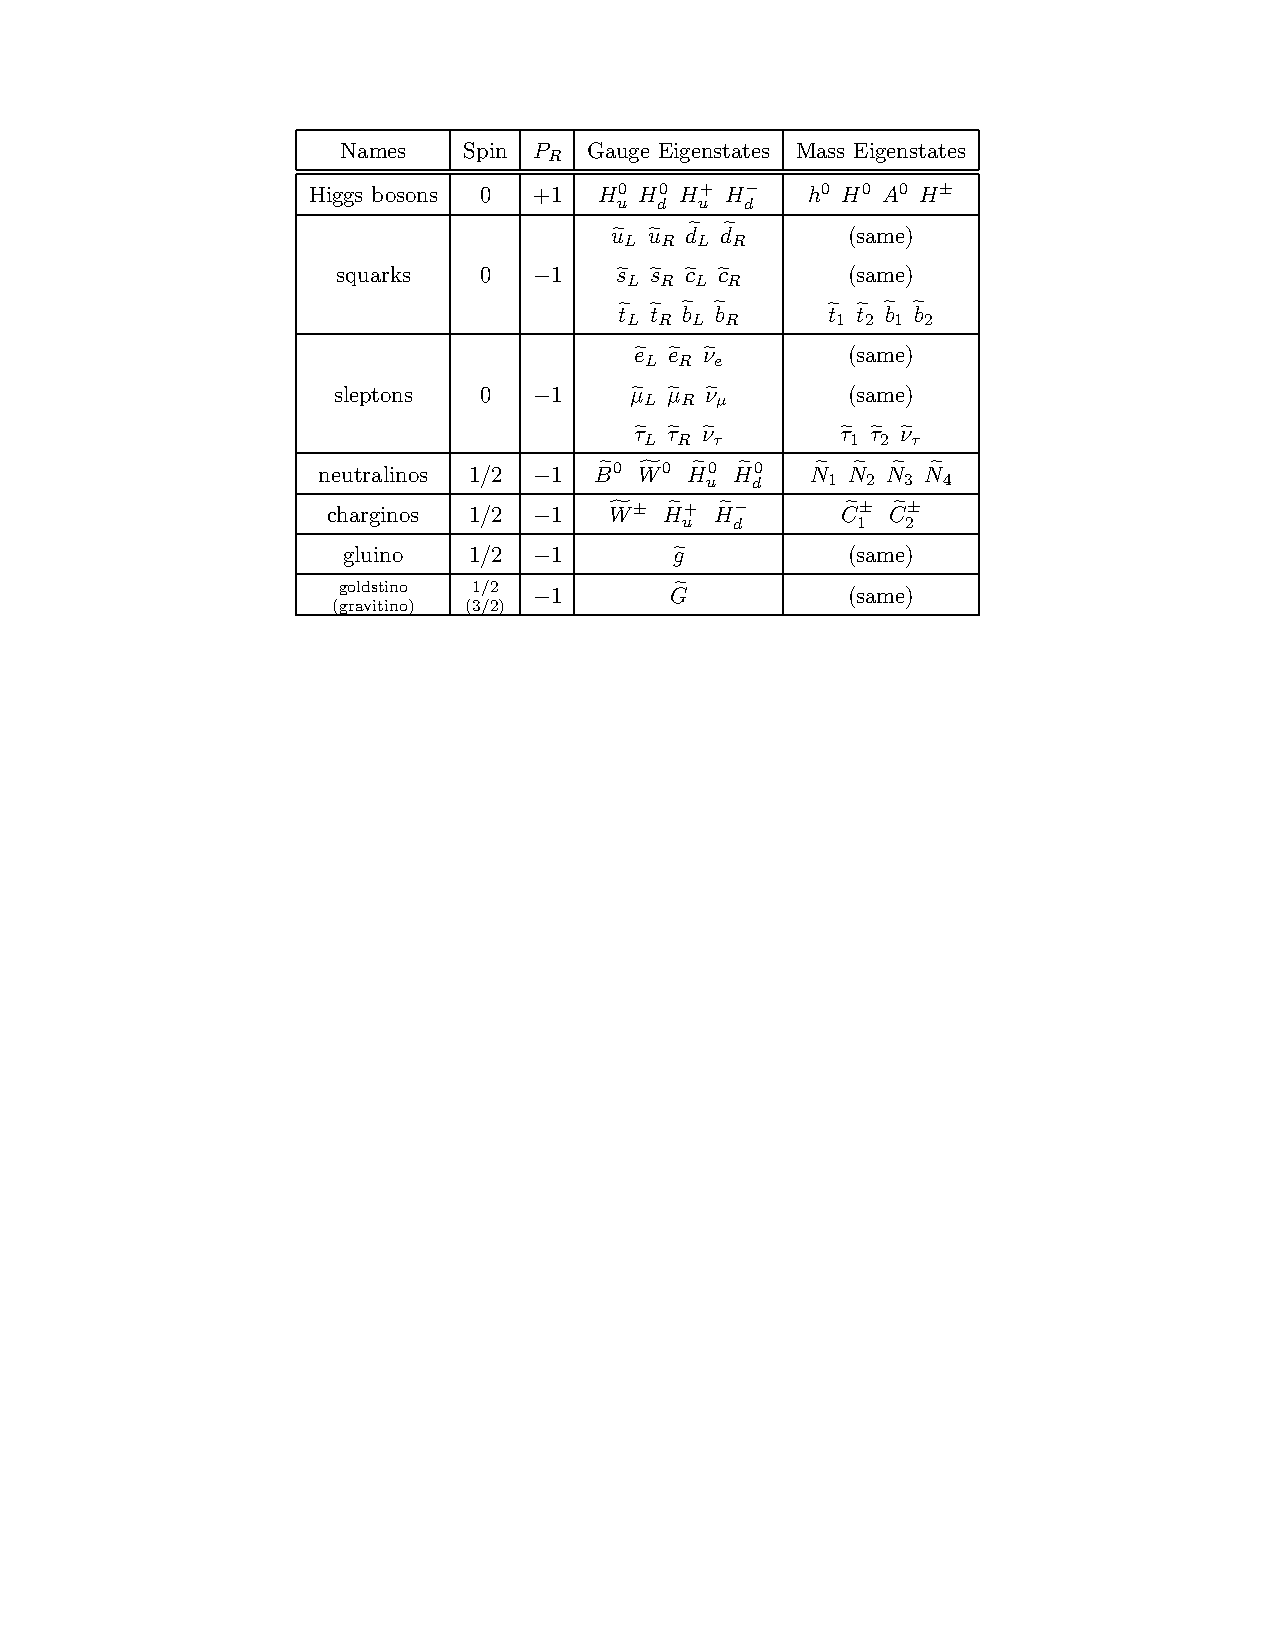
\includegraphics[width=0.7\textwidth]{susy_particles}
\label{fig:susy:susy_particles}
\caption{A table of the various SUSY particles in the MSSM, from~\cite{Martin1997}.}
\end{table}

%%%%%%%%%%%%%%%%  


% From astrophysics observations, we know that a candidate WIMP must be heavy and neutral, so we are interested in the SUSY particles which fit this criterea. In particular, what matters to us is the particular linear combination of $\tilde{B}$, $\tilde{W}^3$, $\tilde{H}_1^0$, and $\tilde{H}_2^0$. The superpotential introduces quadratic couplings between the these four fields when the supersymmetry is broken and after the Higgs particles have acquired a vev and spontaneously broken the remaining symmetry. In particular, the couplings are defined by the mass matrix:
% \begin{align}
%   M_\mathrm{neut}=
% \left(
% \begin{array}{cccc}
%  M_1 & 0 & -c_{\beta } m_z s_w &
%    m_z s_{\beta } s_w \\
%  0 & M_2 & c_{\beta } c_w m_z &
%    -c_w m_z s_{\beta } \\
%  -c_{\beta } m_z s_w & c_{\beta }
%    c_w m_z & 0 & -\mu  \\
%  m_z s_{\beta } s_w & -c_w m_z
%    s_{\beta } & -\mu  & 0
% \end{array}
% \right)  \label{eqn:massx}
% \end{align}
% This matrix is in the $\tilde{B}-\tilde{W}^3-\tilde{H}_1^0-\tilde{H}_2^0$ basis, and diagonalized by a transformation: $M_\mathrm{neut}^\mathrm{diag} = N^\dagger M_\mathrm{neut} N$, where we expect $N$ to appear as a mixing matrix in neutralino interaction terms. From the diagonalization of this matrix, 4 mass eigenstates appear, labelled $\chi_m^0$ with $m\in\{1,2,3,4\}$ \cite{Jungman}. Heavy neutralinos will decay down the spectrum to the lightest.

% However, it is not immediately clear what makes the $\chi$ a good candidate to be the LSP, as other superparticles could be lighter.  But the Higgsinos have Yukawa couplings to other particles, and in particular the large contributions of top loops lead Yukawa couplings to run negative in low energies \cite[p.~80]{Martin1997}. While the exact values of the runnings are of course very model dependent, Figure~\ref{fig:mass-run} gives an example of this sort of running \cite[p.~80]{Martin1997}. The dominant effect on $M_1$ is indeed the top-Yukawa coupling which pulls down the mass below others, whereas SU(3) couplings pull the mass of squarks much higher, for example \cite[p.~81]{Martin1997}.



% Writing out the mixing parameters explicitly, we thus have:
% \begin{align}
%   \chi = N_{10}^* \tilde{B} + N_{20}^* \tilde{W}^3 + N_{30}^* \tilde{H}_1^0 + N_{40}^* \tilde{H}_2^0
% \end{align}
% where $N$ is the neutralino mixing matrix which arises from the diagonalization of the mass matrix in eqn. \ref{eqn:massx}. 

% We have shown, then, that $MSSM$ produces a wide variety of new particles when we write down an initial unbroken Lagrangian using superfields that must be invariant under SUSY transformations. Soft, explicit breaking of the supersymmetry introduces additional couplings; combined with the couplings in the superfields themselves, we generate a mass matrix $M_\mathrm{neut}$ which couples the Higgsinos, Bino, and Wino fields. Diagonalizing this matrix leads to new mass eigenstates, the neutralinos $\chi$. The lightest of these is a good candidate to be the LSP, as RG running of masses makes most other particles much heavier at energies below the supersymmetry breaking scale.



\subsection{Fixing Naturalness}

We began exploring SUSY to fix the holes of the Standard Model. The most pressing of these\footnote{Obviously this is a matter of personal taste, though certainly to me this is the largest concern with the Standard Model as it stands.} was the naturalness issue, where diverging top loops in the Higgs boson mass renormalization required incredibly precise fine-tuning to cancel, as described in Section~\ref{chapter:susy:problems:naturalness}. How does SUSY solve this issue?

%%%%%%%%%%%%%%%%

\begin{figure}
\centering
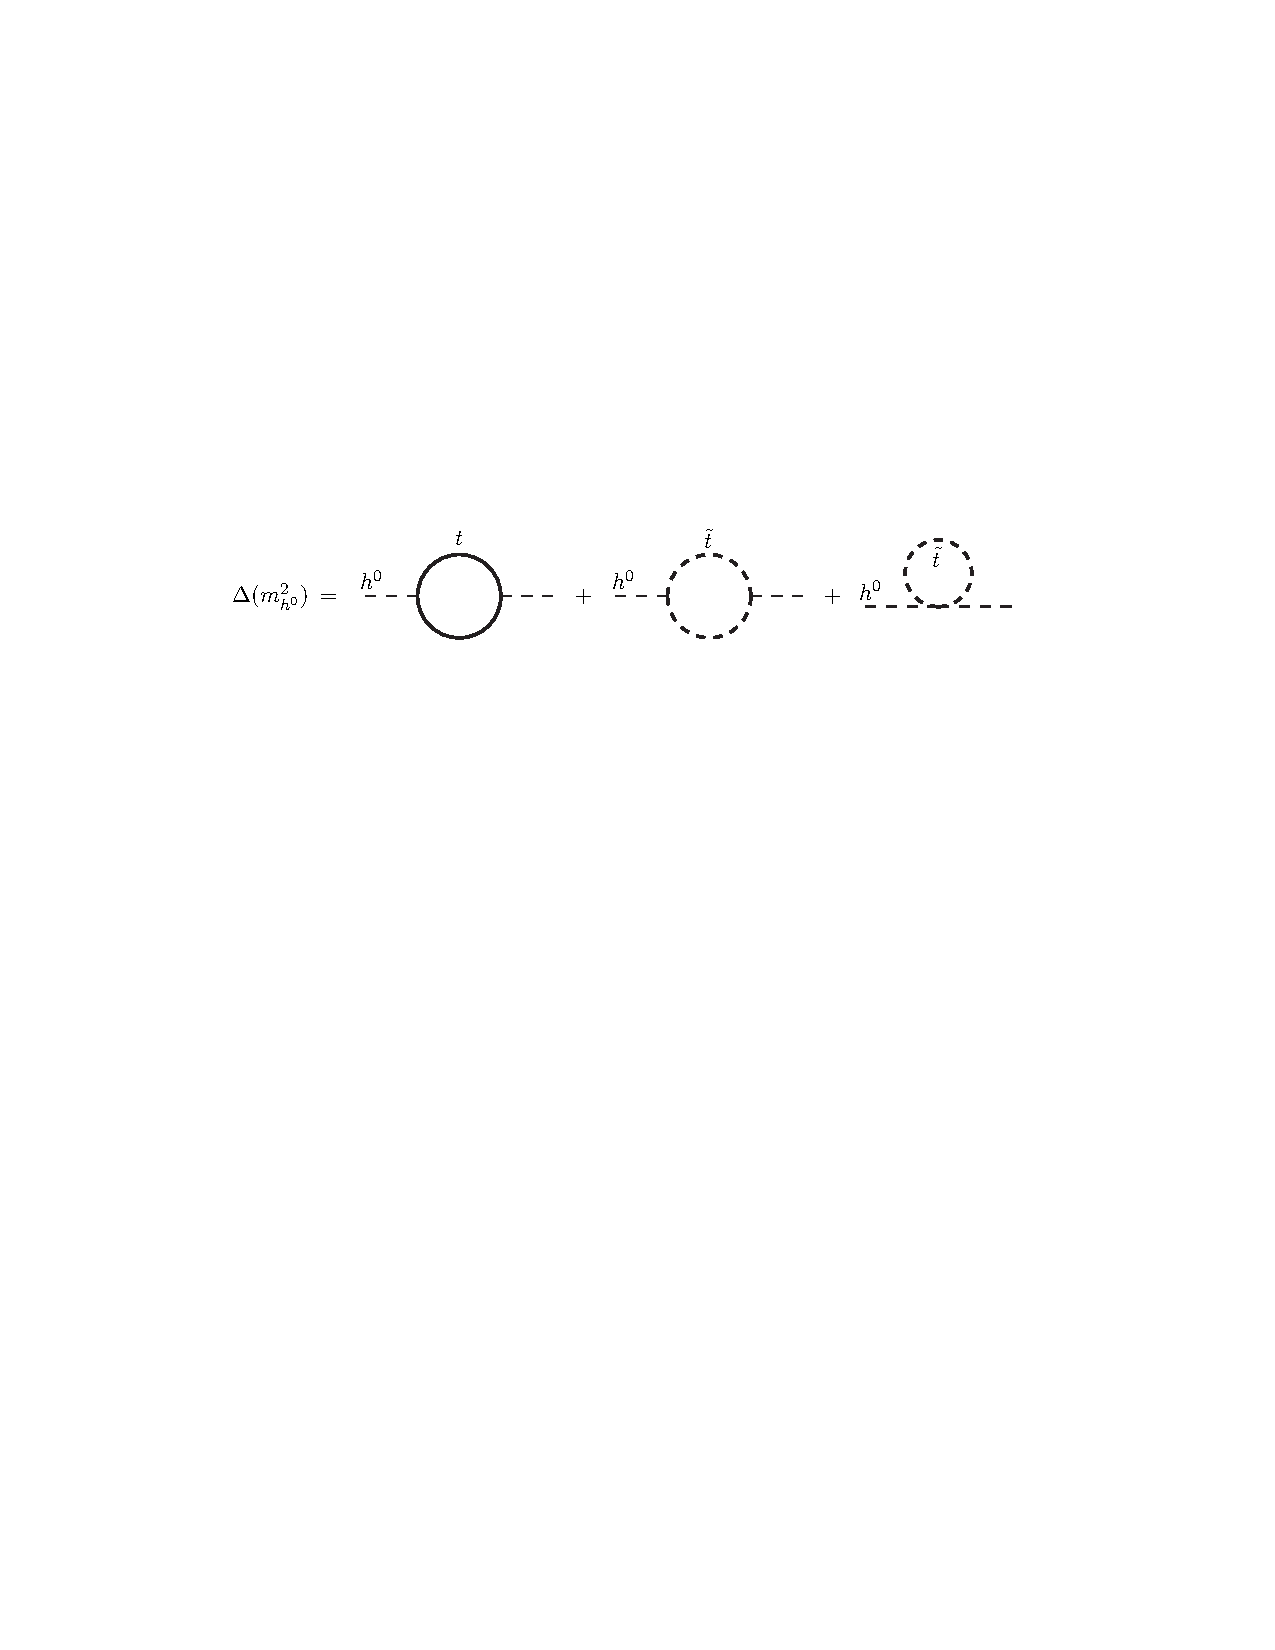
\includegraphics[width=0.7\textwidth]{higgs-loop-cancel}
\label{fig:susy:higgs-loop-cancel}
\caption{A schematic diagram of the top quark and stop squark loops involved in renormalizing the Higgs mass in SUSY, from~\cite{Martin1997}.}
\end{figure}

%%%%%%%%%%%%%%%%  

In SUSY, the top is not the only particle which contributes heavily to the mass renormalization of the Higgs: the \textit{stop squarks}, because of their supersymmetry with top quarks, have the exact same coupling to the Higgs. The complete set of diagrams that contibute is displayed in Figure~\ref{fig:susy:higgs-loop-cancel}. The solution here lies in the fact that boson and fermion loops come in with an opposite sign: this rule is often referred to as the ``Fermi minus sign'', and it means that the stop quark and top quark loops go in opposite directions. Both of these are formally infinite, but can cancel up a value proportional to the mass of stops and tops: \cite{Martin1997}
%
\begin{equation}
\Delta(m_{h^0}^2) = \frac{3}{4\pi^2} \cos^2 \alpha y_t^2 m_t^2 \ln \left( m_{\tilde{t}_1} m_{\tilde{t}_2} \right),
\end{equation}
%
where $\alpha$ is a mixing angle related to the SUSY Higgs sector, and $y_t$ is the top Yukawa coupling.

The corrections are finite, and naturalness was restored--- and all we needed was a light stop squark~\cite{Dimopoulos:1981zb,Witten:1981nf,Dine:1981za,Dimopoulos:1981au,Sakai:1981gr,Kaul:1981hi}! Unfortunately, the situation is not quite so simple: the stop itself is a scalar and undergoes similar mass renormalization as the Higgs~\cite{natural}. In particular, the previously alluded to gluino, because of its color charge, couples especially strongly to the stop squark in this loop and dominates the mass renormalization. In particular, it pulls the mass of the stop squark \textit{up} as~\cite{natural}:
%
\begin{equation}
\partial_t m_{\tilde{t}}^2 = - \frac{8\alpha_s}{3\pi} M_3^2
\end{equation}
%
where $M_3$ is the mass of the gluino in the IR and the $t = \log \mu$. This consequence of this, after solving the renormalization group equations, are that the stop should have about half the mass of the gluino--- or else very specific tree-level initial values are required keep the stop mass lighter. Thus, in addition to light stops, our theory should also have light gluinos~\cite{natural}.

The story is not completely finished yet--- the Higgsinos also contribute, since the Higgs and the Higgsinos should have similar masses. The Higgsinos form a component of the Neutralino, so this means that the \lsp should not be too heavy either~\cite{natural}.


\subsubsection{Model Building, and Simplified Models}

Our efforts to impose naturalness with SUSY have run into a few complications, but the situation is still rather simple. Our requirements for natural, un-tuned models are:
%
\begin{itemize}
\item Light stops in order to cancel the divergent top loops in the Higgs mass renormalization
\item Light gluinos because of the radiative corrections to the stop mass
\item Light neutralinos because of the relationship between the Higgs and Higgsinos
\end{itemize}
%
What about the other SUSY particles--- the squarks, the sleptons, and so forth? A full SUSY model will likely have them, but for the sake of experimental analyses, a \textit{simplified model} approach can be adopted~\cite{simplified}. In these models, a minimal set of particles related to a particular observable signature is kept at low mass; all the other particles are set to high masses, and are effectively integrated out using an Effective Field Theory approach. We can use this philosophy in considering our minimal set of required particles: others can exist, but have a much smaller effect on the physics of naturalness, and so we essentially ignore them.


An important question remains for the model: how will the new physics actually be produced? It is possible, for example, to directly produce pairs of \lsp's and search for such a signature immediately, but another attractive option goes back to the gauge couplings of the squarks and gluino. In particular, the LHC is a hadron collider and therefore is colliding quarks and gluons: production of particles which strongly couple to quarks and gluons is therefore expected to be enhanced. The \lsp has no such coupling, but the squarks do, and the gluino, because of its higher color charge, has an even larger coupling. Figure~\ref{fig:susy:multi_strong} shows the production cross-sections for gluions, squarks, and stops alone: the higher multiplicity of treating squarks inclusively (as well as $t$-channel production which is possible for the light flavors) raises their production over that of stops alone, but the gluinos have the highest cross-section of all. 

%%%%%%%%%%%%%%%%

\begin{figure}
\centering
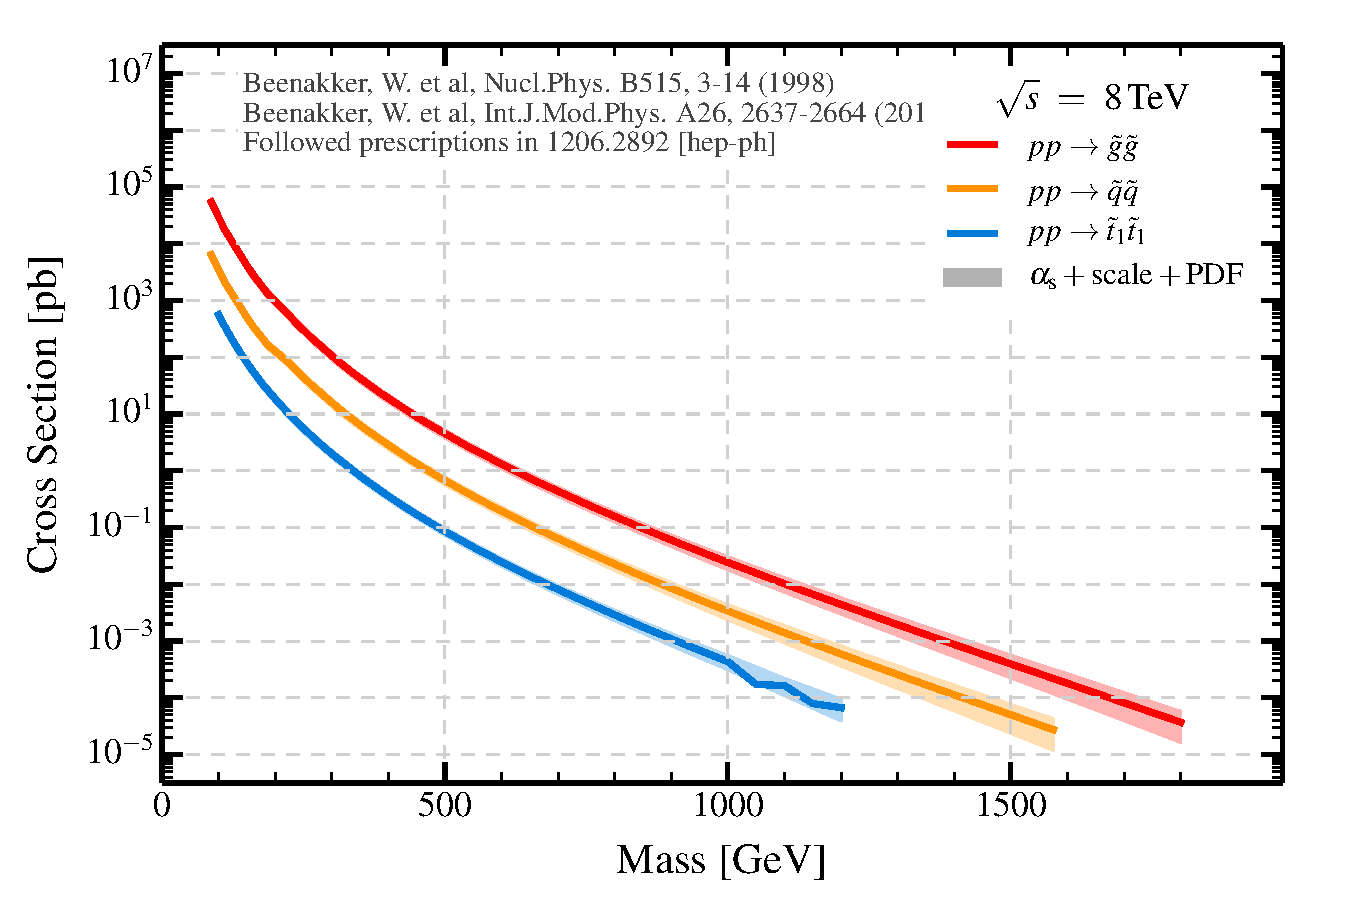
\includegraphics[width=0.7\textwidth]{multi_strong-2.pdf}
\label{fig:susy:multi_strong}
\caption{The production cross-section of various strongly interacting SUSY particles. From ATLAS SUSY group.}
\end{figure}

%%%%%%%%%%%%%%%%  

How do all of these requirements fit together? Figure~\ref{fig:susy:gtt} gives an example of the Feynman diagrams which combine all of these various requirements. Gluino pair production is used as the production mode, as it has the largest cross-section. Stops are the lightest squarks, and are either heavier than the gluino (in which case the decay to the \lsp is off-shell), or lighter than the gluino. The final states are filled with top quarks and large missing energy from the \lsp. Figure~\ref{fig:susy:spectra} shows an example of possible masses of particles in these models.


%%%%%%%%%%%%%%%%%%%%%

\begin{figure}
\centering
\subfigure[Off-shell stop]{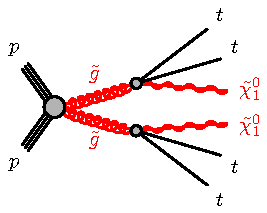
\includegraphics[width=0.45\textwidth]{gogo-ttttN1N1.pdf}}
\subfigure[On-shell stop]{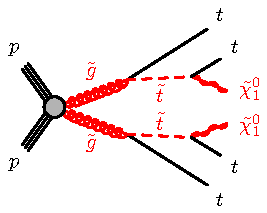
\includegraphics[width=0.45\textwidth]{gogo-ttttN1N1-stst.pdf}}
\label{fig:susy:gtt}
\caption{Feynman diagrams for natural SUSY processes at the LHC, in the case of off-shell stops and on-shell stops.}
\end{figure}

%%%%%%%%%%%%%%%%%%%%%


%%%%%%%%%%%%%%%%

\begin{figure}
\centering
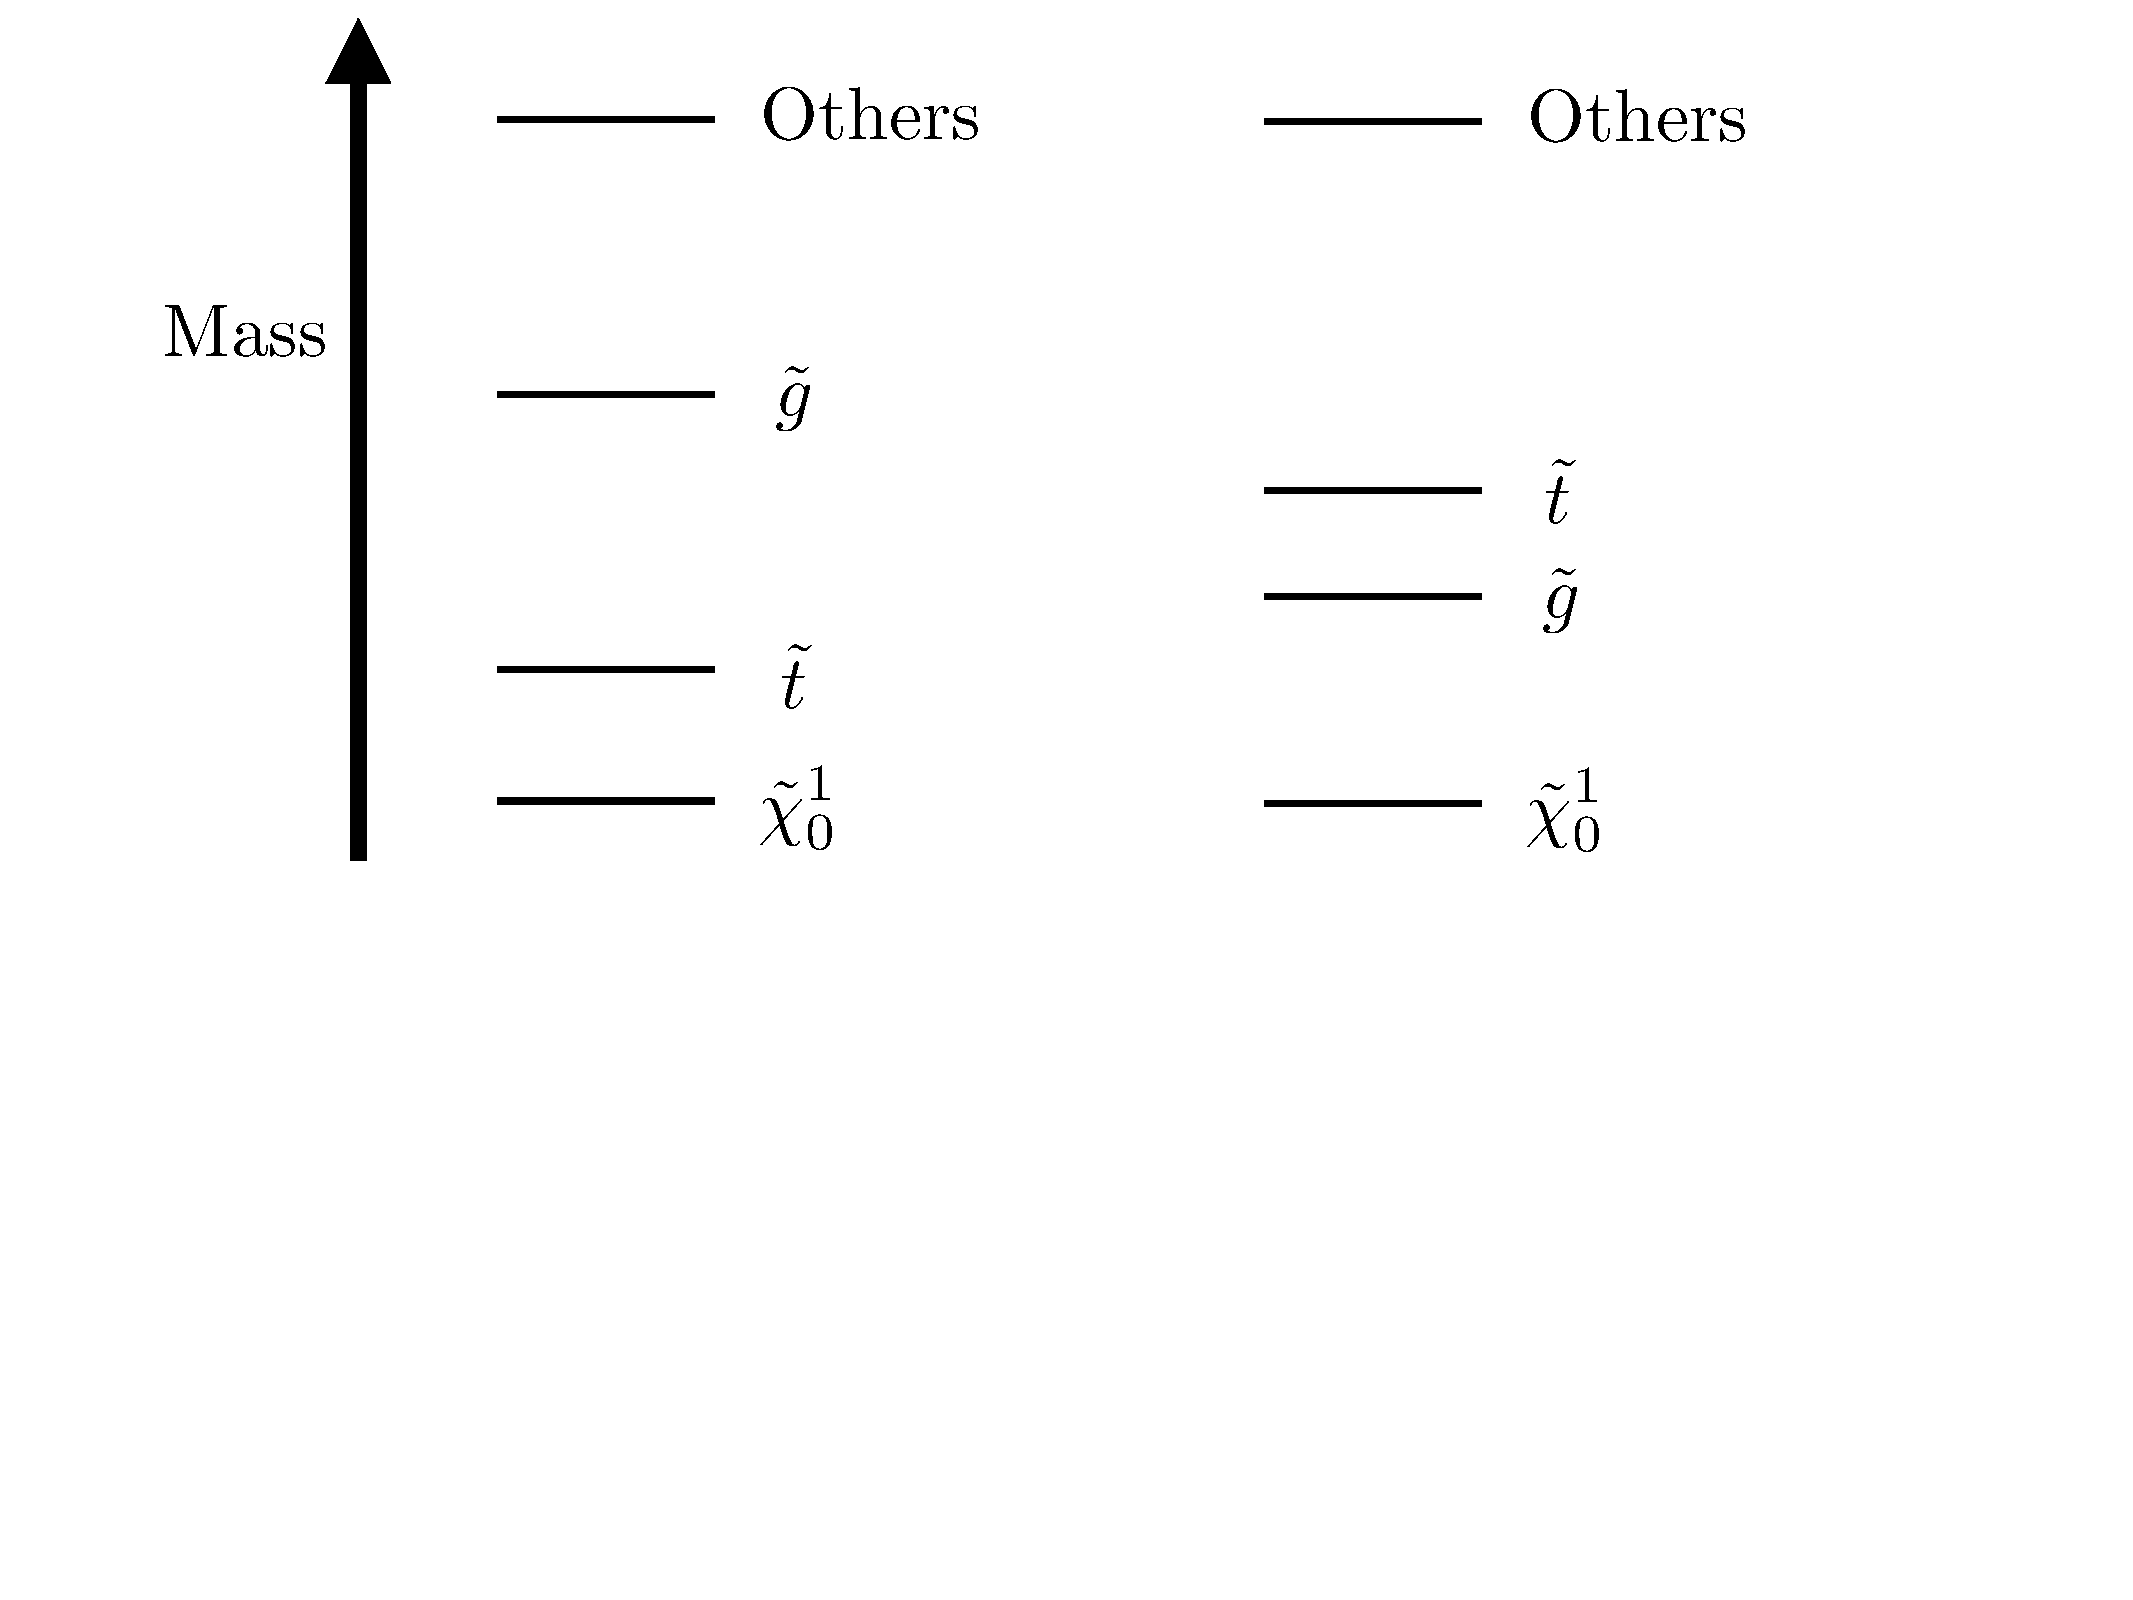
\includegraphics[width=0.7\textwidth]{spectra.pdf}
\label{fig:susy:spectra}
\caption{Examples of SUSY simplified model spectra which satisfy the requirements of naturalness.}
\end{figure}

%%%%%%%%%%%%%%%%  

%spectra

%diagram from martin

%gluino suck

\subsection{Coupling Unification}

% plot from hitoshi; quote some of the changes to \beta functions

It turns out that SUSY fixes more than just the naturalness issue of the Standard Model: it also changes the evolution of the coupling constants to suggest that all the forces unify, as seen in Figure~\ref{fig:susy:couplings_mssm}~\cite{susypheno,SUSYUnification}. Is this meaningful, or a coincidence? It is hard to tell, since the unification scale of $\mu \approx 10^{16}$~GeV is well outside experimental access.

%%%%%%%%%%%%%%%%

\begin{figure}
\centering
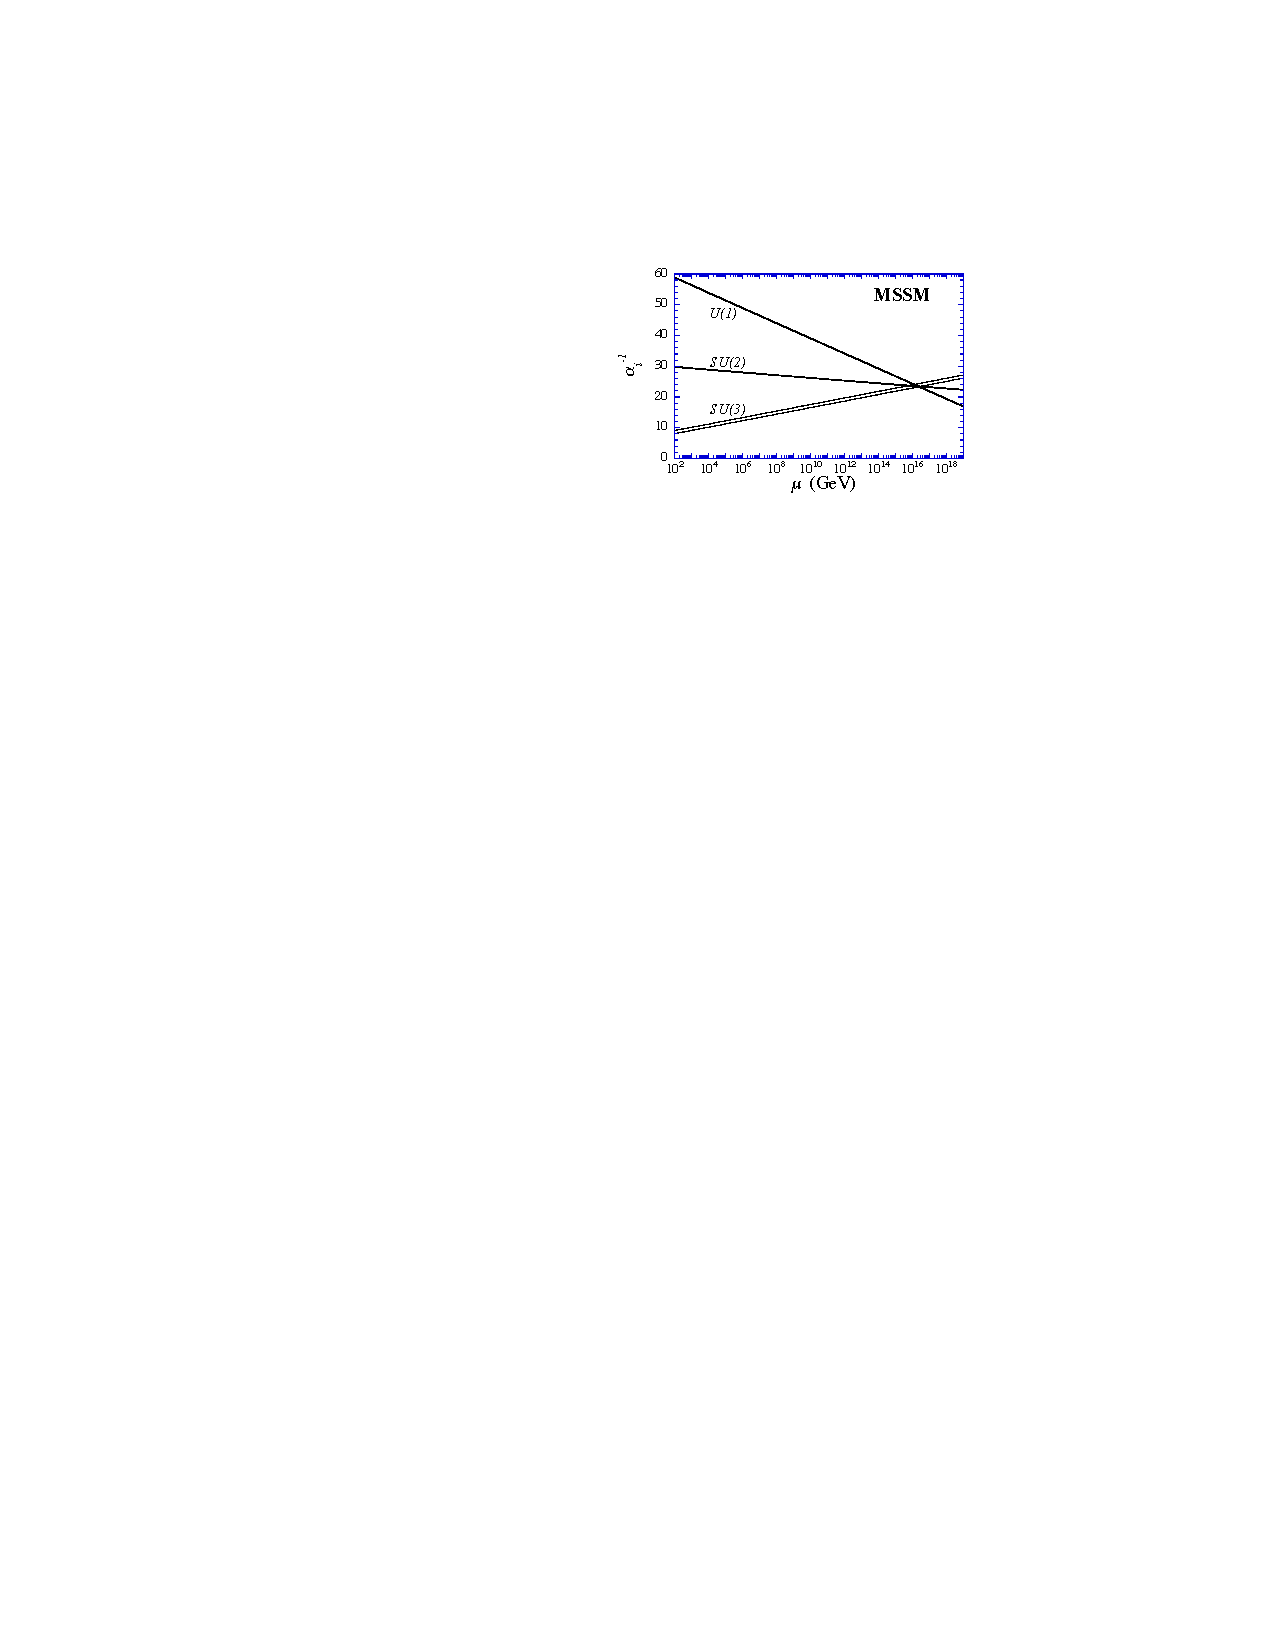
\includegraphics[width=0.7\textwidth]{couplings_mssm.pdf}
\label{fig:susy:couplings_mssm}
\caption{The evolution of the strength of the coupling constants of the three symmetry groups of the SM, in the MSSM. They clearly all meet at one point, suggesting that a large symmetry group would be able to unify them at the $\mu = 10^{16}$~GeV mass scale. Figure from \cite{susypheno}.}
\end{figure}

%%%%%%%%%%%%%%%%  

\subsection{Dark Matter}

Finally, we turn to the subject of the missing matter in the universe: dark matter. In our earlier construction of the model, we had assumped the presence of $R$-parity, which guaranteed the stability of the LSP\footnote{It is easy to see what this guarantees LSP stability, as it requires all interactions are guaranteed to couple an even number of supersymmetric particles and one SM particle. This means that moving down a mass cascade, a heavy SUSY particle can decay to lighter SUSY particles and SM particles, but the lightest is stable.}. For reasons of naturalness, we have already required a light neutralino \lsp, but this particle has other attractive properties. It is electromagnetically neutral, and interacts only via the weak nuclear force: this makes it a perfect candidate to be the Weakly Interactive Massive Particle (WIMP) preferred by large-scale galactic simulations~\cite{Goldberg:1983nd,Ellis:1983ew,Jungman}.

Since the \lsp is expected to be stable, there should be a number of them left over from production in the Big Bang. The density is defined by the rates of annihilation ($\chi\overline{\chi} \rightarrow l \overline{l}$) and production ($l\overline{l}\rightarrow \chi\overline{\chi}$. As the universe cools, eventually the annihilation rate falls below that of the expansion rate of the universe, thereby freezing out the mechanisms which maintain thermal equilibrium and leaving a ``relic'' cosmological abundance \cite{Jungman}.The correct description for the number density $n_\chi(t)$ out of equilibrium is given by the Boltzmann equation:
\begin{align}
  \df{n_\chi}{t} + 3 H n_\chi = - \langle \s_A \nu \rangle [(n_\chi)^2 - (n_\chi^\mathrm{equi})^2]\label{eqn:boltz}
\end{align}
where $H=\dot{a}/a$ is the Hubble expansion rate, $\langle\sigma_a \nu\rangle$ is the thermally averaged cross-section, $a$ is the scale factor, and $n_\chi^\mathrm{equi}$ is the thermal equilibrium distribution, given by either the Fermi-Dirac or Bose-Einstein distribution. The second term on the left corresponds to the expansion of the universe; number changing interactions provide the terms on the right hand side, as the first term accounts for depletion from annihilation and the second comes from creation from inverse annihilation. 

Solving this equation leads to a prediction for the thermal relic of this new particle with mass near the electroweak scale. The ``Dark Matter Miracle'', is that an appropriate value for the annihilation cross section, $\langle \sigma_A \nu \rangle \sim \alpha^2 (100~\mathrm{GeV})\sim 10^{-25}~\mathrm{cm}^3\mathrm{s}^{-1}$, is predicted just based on the idea of this new particle existing at the electroweak scale. This value gives the approximately measured density of dark matter as seen by measurements (rotation curves, etc.) and simulation (large-scale structure). 

SUSY provides a candidate a compelling candidate for WIMP Dark Matter with the neutralino \lsp, which we have already required to have a mass near the electroweak breaking scale for the sake of naturalness. Another hole in the Standard Model is thus miraculously solved by SUSY--- it is clear why this theory has gathered so much interest from theorists and experimentalists over the years.

\section{The Status of SUSY after LHC Run 1}
\label{chapter:susy:status}

%stop and gluino limits
With Run 1 of the LHC coming to a close, an extremely detailed program  of searches for SUSY at the ATLAS detector has been finished~\cite{Atlassusy1lepton,susyoleptons,Aad:2011ks,SUSYZeroLep2011,SUSYOnelep2011,SUSYJetMult2011,SUSYTwoLep2011,SUSYStopGluino2010,Aad:2013wta,Aad:2014lra}. Unfortunately, none of these analyses have seen any excesses beyond the expectation of SM production\footnote{With the exception of one $3\sigma$ excess in \cite{Aad:2015wqa}, though perhaps one fluctuation in such a large dataset is expected.}. Figure~\ref{fig:susy:limits} shows the limits on production in two particularly relevant sets of analyses: the search for direct production of stop quarks which decay to neutralinos, and the production of gluinos which decay through stop quarks to neutralinos. These are exactly the simplified models we have been earlier motivated by with our concerns about naturalness, but with no excesses in sight in these channels, even SUSY starts to require significant artificial tuning.



\begin{figure}[htbp]
  \centering
    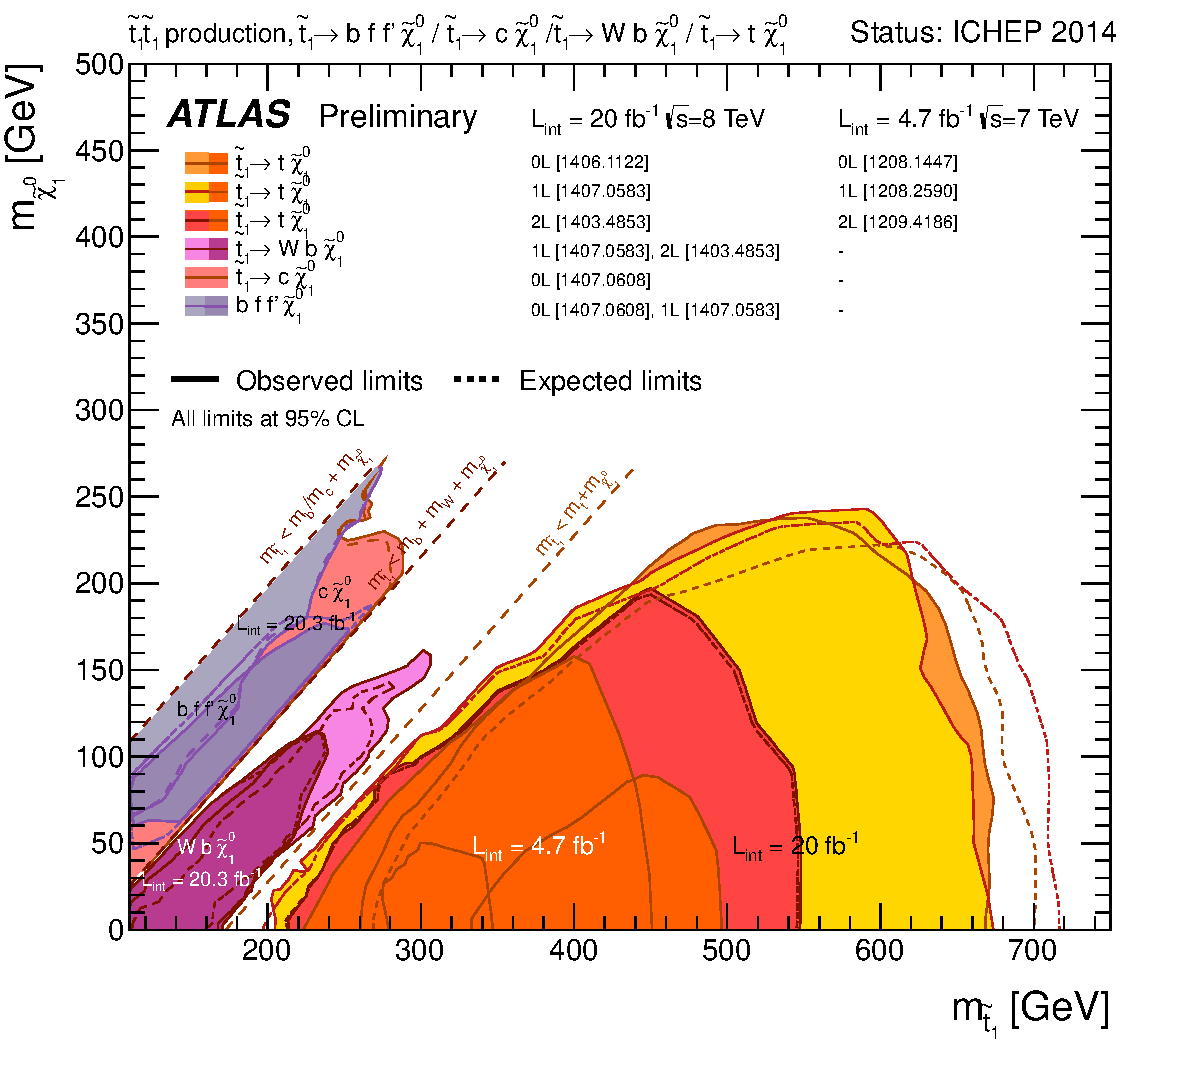
\includegraphics[width=0.45\textwidth]{ATLAS_SUSY_Stop_tLSP}
    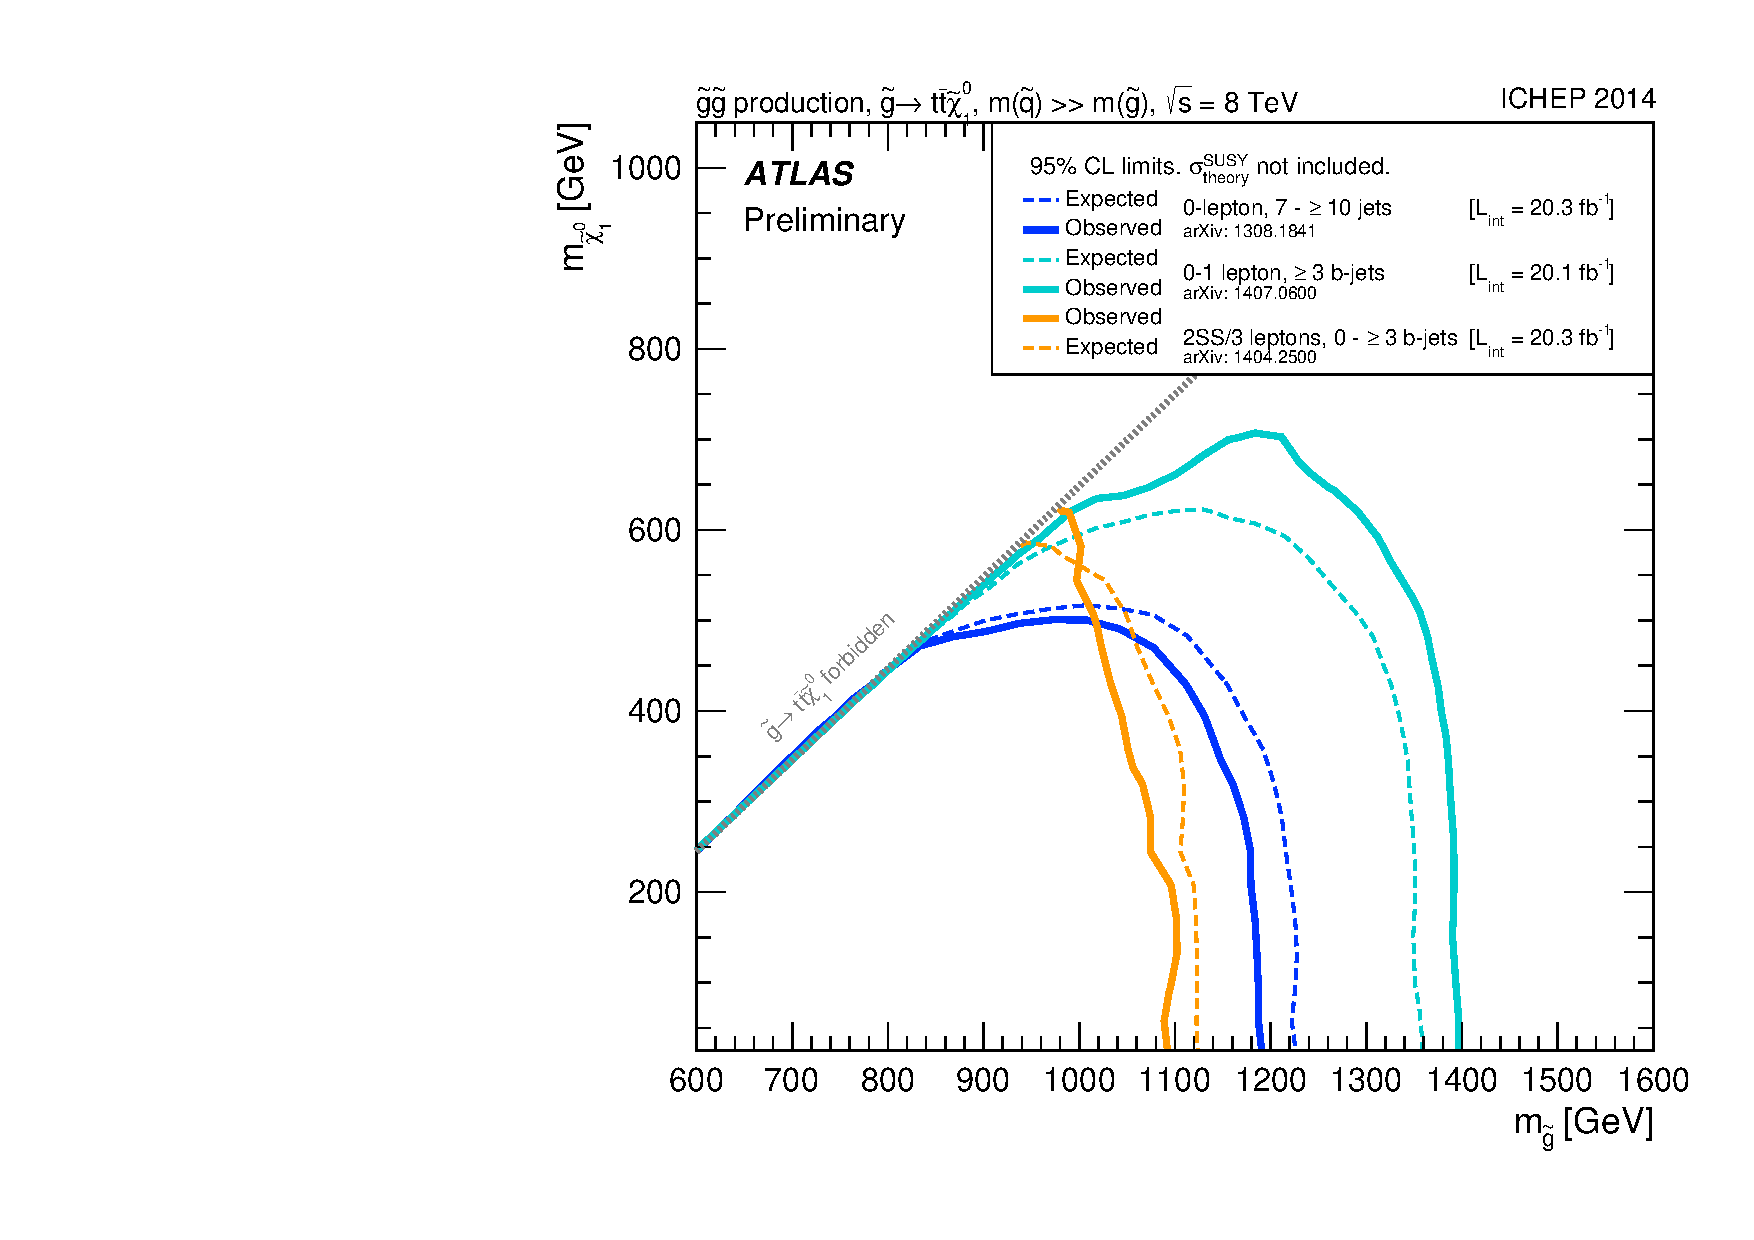
\includegraphics[width=0.45\textwidth]{ATLAS_SUSY_Gtt}
  \caption{The limits on SUSY particles in the $\tilde{t}-\lsp$ (left) and $\tilde{g}-\lsp$ (right, with $\tilde{t}$ as lightest squarks). Stops are excluded to 700 GeV, and gluinos to 1.4 TeV, severely stressing the hopes of naturalness.}
  \label{fig:susy:limits}
\end{figure}


\subsection{Assumptions}

A relevant question to ask at this point is whether there is an underlying assumption in the experimental searches which is crippling our search for SUSY. Is one of our theoretical requirements biasing our approach to searching for new physics?

Consider the requirement of the stop quark being light--- while the searches in Figure~\ref{fig:susy:limits} require the experimental signatures related to stops (i.e., top quarks in the final state), many other searches exists which assume only light flavor squarks are dominantly produced. These searches too see no hints of new physics.

This leads us to the assumption of the light \lsp, and its stability. Figure~\ref{fig:susy:meff} shows an example of one search and the variables used in it. This variable, $m_{\rm eff}$, is composed as the sum of \met and \Ht in an event: because of the stability and weakly-interacting nature of the \lsp, it does not interact with the detector and therefore appears as missing energy. Almost every ATLAS SUSY search makes this assumption, and uses variables related to the \met to construct their searches. 
 
%%%%%%%%%%%%%%%%

\begin{figure}
\centering
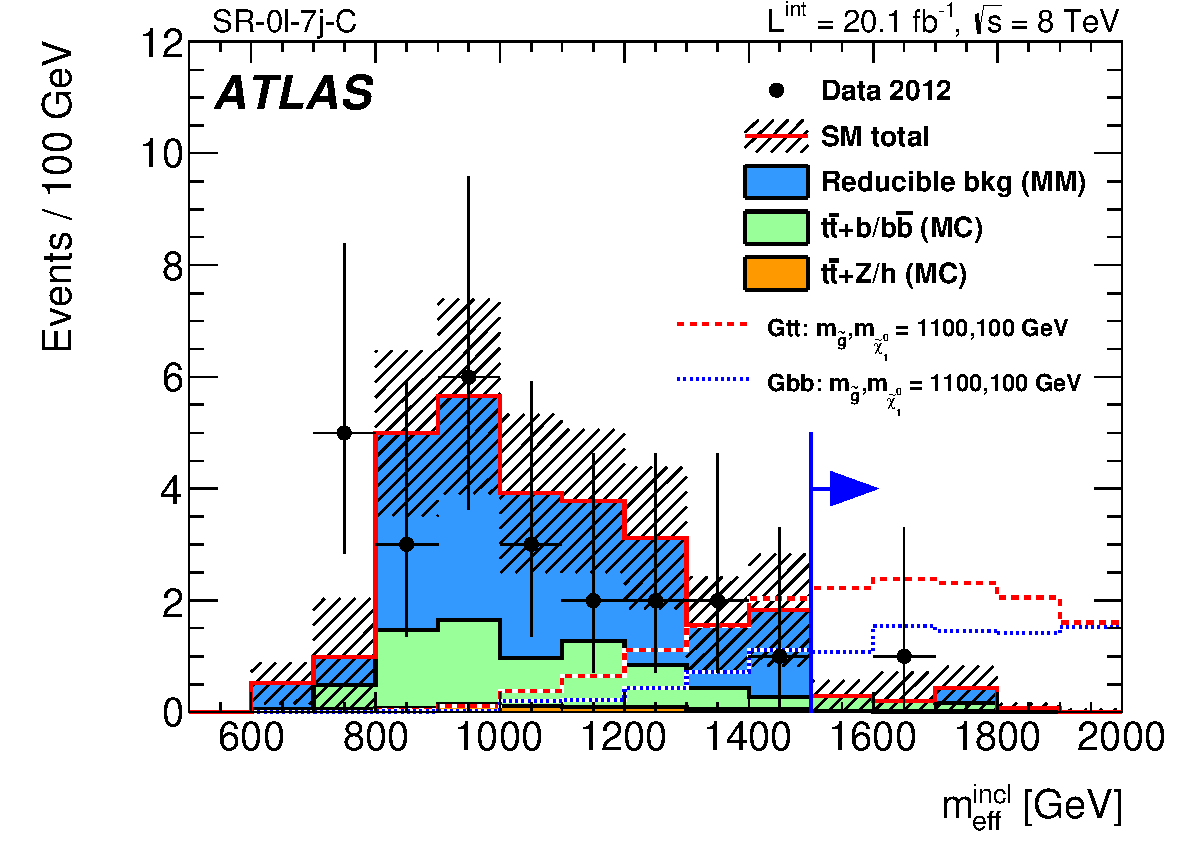
\includegraphics[width=0.7\textwidth]{meff.pdf}
\label{fig:susy:meff}
\caption{The $m_{eff}$, or the sum of \met and \Ht in an event, used in a search for gluinos decaying through stop squarks. From \cite{Aad:2014lra}.}
\end{figure}

%%%%%%%%%%%%%%%%  

This assumption motivates us to reconsider the statement of $R$-parity we began with. Is it possible to remove this symmetry from the model, thereby allowing the \lsp to decay to SM particles? Are there any other experimental limits that prevent this? 

\section{$R$-Parity, and How to Violate It}
\label{chapter:susy:r}
		 % from martin
Earlier in Section~\ref{chapter:susy:susy:developing}, we assumed the presence of a $R$-parity, defined as $R_p = (-1)^{3(B-L)+2S}$. This eliminated the following terms from the potential~\cite{dreinerRPV}:
%
%---------------------
  \begin{eqnarray} 
    \Wrpv &= \frac{1}{2} \lamijk L_{i}L_{j}\Ebar_{k} + \lampijk L_{i}Q_{j}\Dbar_{k} +  \nonumber \\
       & \quad \frac{1}{2}\lamppijk\Ubar_{i}\Dbar_{j}\Dbar_{k} + \kappa_iL_{i}H_{2},
    \label{eqn:rpvandudd:wrpv}
  \end{eqnarray} 
%---------------------

\noindent where $i,j,k=1,2,3$ are generation indices (which may be ommitted from the discussion below if the statements do not depend on generation). The last term, referred as the the bilinear coupling, can be removed from the theory by a rotation of the $L$ and $H$ superfields, and so is commonly ignored~\cite{dreinerRPV}. The first three trilinear terms, with Yukawa couplings for each term are given by \lam, \lamp, and \lampp, are generally non-trivial. The particle content with these new terms is identical to that of $R$-parity conserving (RPC) models, but the $R$-parity violating (RPV) terms add new interactions.

The structure of these interactions couples one supersymmetric particle together with two SM particles. This has many experimental consequences, not only in the signatures in colliders, but also in the interactions of SM particles at low energy. Interactions, such as the one in Figure~\ref{fig:susy:rpv_proton} in which an off-shell squark couples a two quarks to a lepton and a quark, can occur: though suppressed by the mass of the squark in the mediator, such an interaction should occur fairly frequently if $\lamp > 0$ and $\lampp > 0$. In particular, purely on dimensional grounds we can estimate the decay rate of the proton based on this diagram as~\cite{dreinerRPV}:
%
\begin{equation}
\Gamma(P\rightarrow e^+ \pi^0) \approx \frac{\lambda_{11k}^{'2} \lambda_{11k}^{''2}}{16\pi^2 m^4_{\tilde{d}_k}} M_\mathrm{proton}^5
\end{equation} 
%
A host of detectors, starting with the IMB~\cite{Gajewski:1989gh} and Kamiokande~\cite{Regis:2012sn} detectors, were built to study the proton decays predicted by RPV and other theories (primarily Grand Unified Theories which introduced similar operators and lead to $e^+ \pi^0$ final states). These detectors were filled with huge amounts of water--- with $O(10^{31})$ protons--- and were lined with photo-multiplier tubes which could detect the Cerenkov radiation which would have been emitted by the electrons and pions if they were produced in a proton decay. No events were observed in any of these detectors or their upgrades or successors, setting limits on the proton lifetime at $\tau(P\rightarrow e^+ \pi^0) > 10^{32}$ years. Thus, the simplest models of RPV SUSY with large couplings to all $\lambda$ modes are clearly excluded; these are often recast into the RPV space as~\cite{PhysRevD47279}:
%
\begin{eqnarray}
  \lamp_{11k}\cdot\lampp_{11k}\; \lsim\; 10^{-23} \left( \frac{{\msquark}} {100~\gev} \right)^2,
  \label{eqn:rpvandudd:protondecay}
\end{eqnarray}
%
where \msquark is the typical squark mass. 

\begin{figure}
\centering
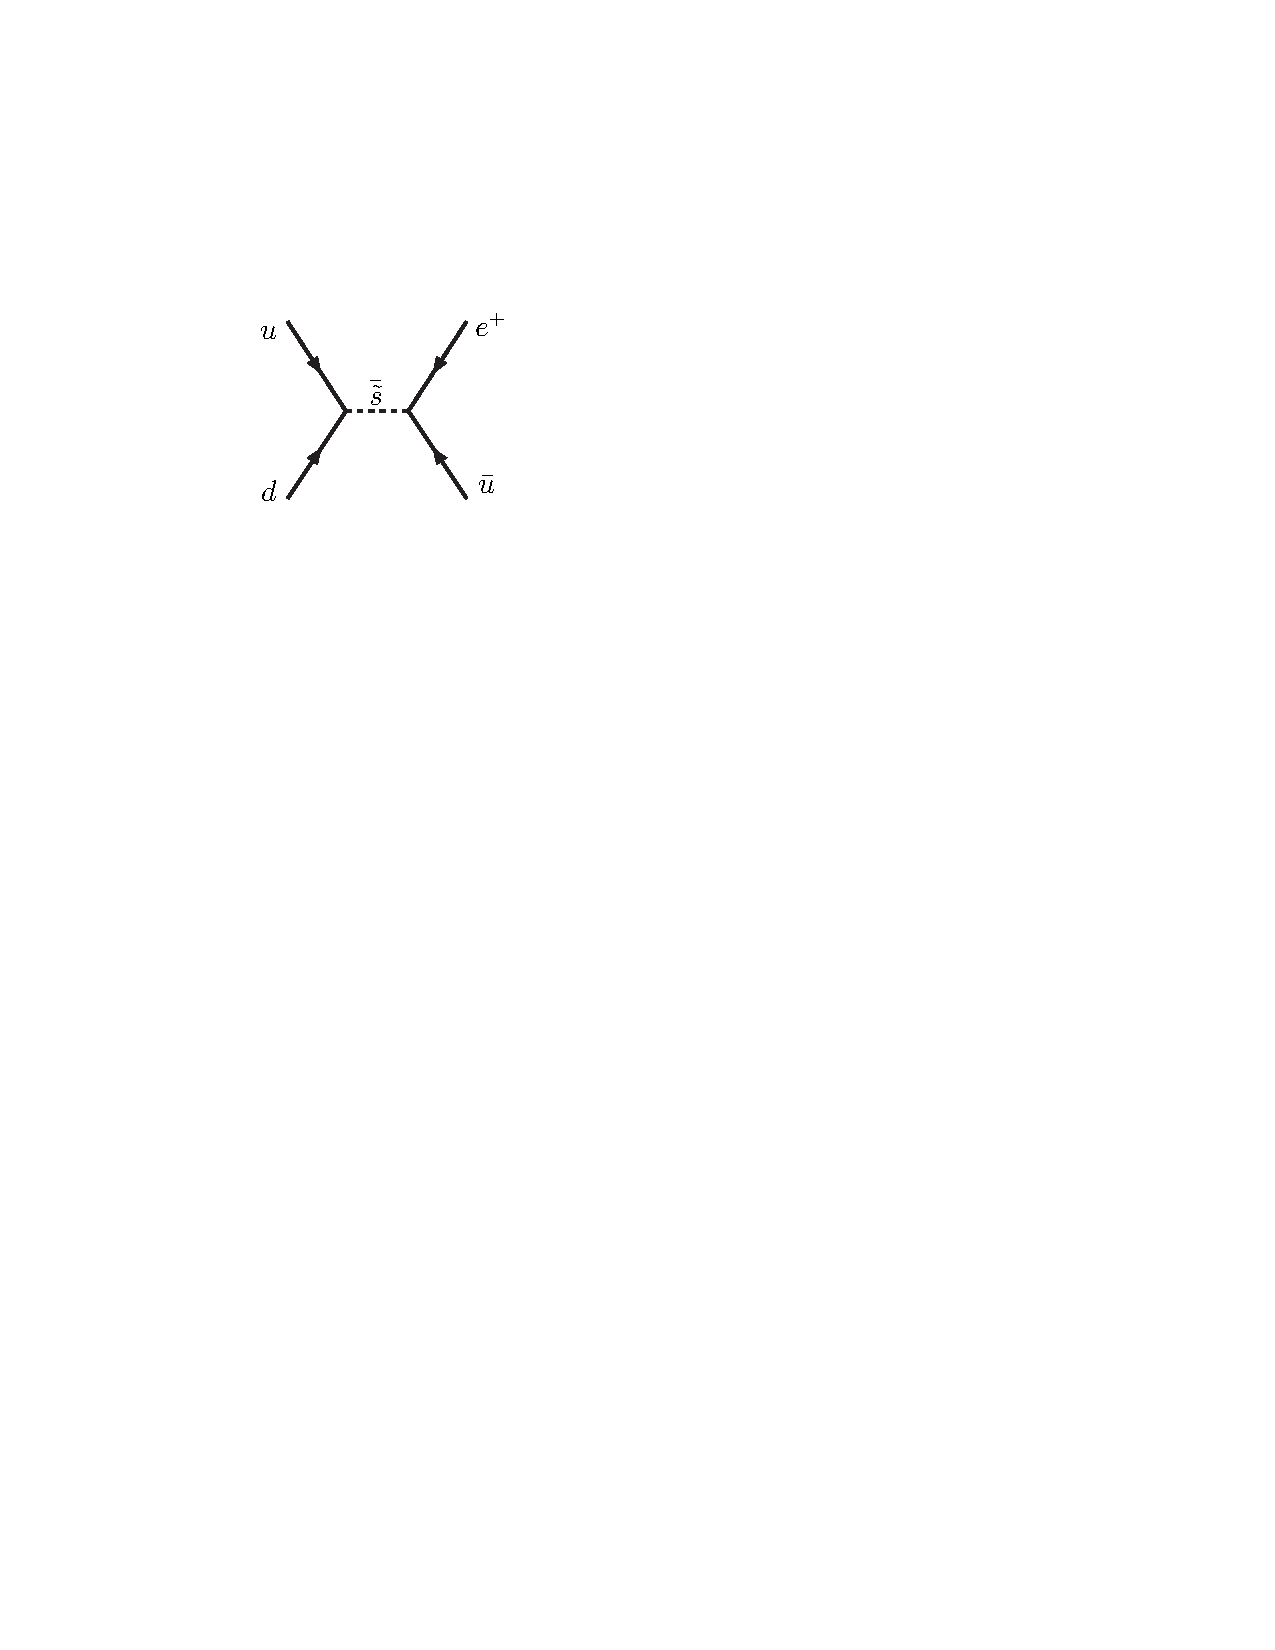
\includegraphics[width=0.5\textwidth]{rpv_proton.pdf}
\label{fig:susy:rpv_proton}
\caption{One example of a diagram which contributes to rapid proton decay in RPV models with $\lampp > 0$ and $\lamp > 0$.}
\end{figure}

This is obviously a very strong restriction, and thus most modern RPV models impose an \textit{ad hoc} condition to require the proton to be stable. This is mostly easily done by requiring that at least one of \lamp or \lampp be exactly equal to zero. If the \lampp term is zero, then the proton stability is clearly preserved, as the off-shell squark in Figure~\ref{fig:susy:rpv_proton} is not able to occur. If $\lam = 0$ and $\lamp = 0$, then $\lampp > 0$ only if the LSP has mass greater than the proton: otherwise, the off-shell squark could decay to an LSP and a quark and the proton could still decay. This is usually a not very strong restriction, however, as the LSP can easily have mass $> 1$~GeV.

The collider signatures of such models are obviously extremely different from RPC scenarios, even if the particle spectrum remains identical. If $\lam > 0$ or $\lamp > 0$, the final states will include leptons instead of the large missing energy tradtionally attributed to the \lsp. Similarly, if $\lampp > 0$, the final states will include many more quarks instead of missing energy. The decay goes through an offshell squark (or slepton), as $\lsp \rightarrow \tilde{q} q$, $\tilde{q}\rightarrow q q$. These signatures are potentially not explored by current LHC analyses, which almost uniformly rely on high missing energy signatures. Figure~\ref{fig:susy:rpv_diagrams} shows several examples of potential models at the LHC: gluino and squark pair production normally has final states dominated with only quarks and missing energy, but these models show the possibility of extra leptons or jets.

% %
% \noindent where \msquark is the typical squark mass. As a result, even when considering this more generic form of the \SUSY superpotential by including \Wrpv, it is still necessary to impose an \textit{ad hoc}, albeit experimentally motivated, symmetry to protect the proton from decay. It is generally necessary that at least one of \lam, \lamp, \lampp be exactly equal to zero. Consequently, it is common to consider each term in Equation~\ref{eqn:rpvandudd:wrpv} independently. In the case of nonzero \lam and \lamp, the typical signature involves leptons in the final state. However, for $\lamppijk \neq 0$, the final state is characterized by jets, either from direct gluino decay or from the cascade decay of the gluino to the lightest neutralino (\ninoone), as also considered here. Because of the structure of Equation~\ref{eqn:rpvandudd:wrpv}, scenarios in which only $\lamppijk \neq 0$ are often referred to as UDD scenarios.


% Current indirect experimental constraints~\cite{Allanach:1999ic} on the sizes of each of the UDD couplings \lamppijk from sources other than proton decay are valid primarily for low squark masses, as suggested by Equation~\ref{eqn:rpvandudd:protondecay}. Those limits are driven by double nucleon decay~\cite{Sher:1994sp} (for $\lampp_{112}$), neutron oscillations~\cite{Zwirner1983103} (for $\lampp_{113}$), and $Z$ boson branching ratios~\cite{Bhattacharyya:1997vv}.

%%%%%%%%%%%%%%%%%%%%%

\begin{figure}
\centering
\subfigure[$\lam> 0$]{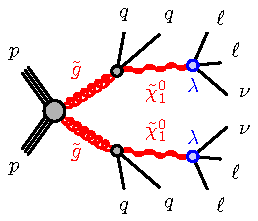
\includegraphics[width=0.45\textwidth]{gogo-qqqqllllvv-RPV.pdf}}
\subfigure[$\lamp > 0$]{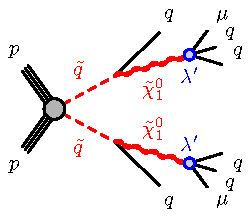
\includegraphics[width=0.45\textwidth]{sqsq-qqlqql-N1N1-RPV.pdf}}\\
\subfigure[$\lampp > 0$]{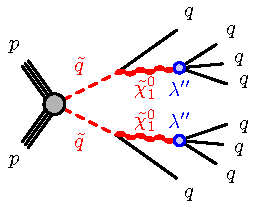
\includegraphics[width=0.45\textwidth]{sqsq-4q4q-RPV.pdf}}
\label{fig:susy:rpv_diagrams}
\caption{Feynman diagrams for several RPV processes at the LHC, each with a different $\lambda$ operator set to $>0$.}
\end{figure}

%%%%%%%%%%%%%%%%%%%%%

It should be noted that the lifetime of the \lsp is proportional to the $\lambda$ terms squared, and inversely proportional to the mass of the squark to the fourth. For particular combinations of these values, it is thus possible for the \lsp to have a significant lifetime and therefore to proceed through the detector some distance before decaying. This can lead to a spectacular displaced signature, which again would be missed by most SUSY searches~\cite{Graham:2012th}. 


\section{Conclusions}

In summary, SUSY is a strongly compelling theory of BSM physics. Its solution to the naturalness problem--- the introduction of a boson/fermion symmetry--- is effective and simple. It furthermore allows for the unification of forces at high energy. And finally, it produces a miraculous dark matter candidate in the form of the \lsp.

Unfortunately, given the results from the first run of the LHC, it is time to reconsider whether we can have all three miracles at once. The least explored space of possibilities exist in the realm of $R$-parity violating models, which have been largely unexplored because of the difficult signal discrimination and background estimation. Chapter~\ref{chapter:search} presents an innovative new search for exactly such models where $\lampp > 0$: the experimental issues are tackled with the aid of the tools of jet substructure developed in Chapter~\ref{chapter:jets-and-substructure}.


\chapter{The Large Hadron Collider}
%!TEX root = ../swiatlow_thesis.tex
\label{chapter:lhc}

The Large Hadron Collider (LHC) is a 27 km long proton-proton ($pp$) synchotron built on the border of France and Switzerland, near the city of Geneva. The accelerator is nestled beneath mostly bucolic French farmland, as seen in Figure~\ref{fig:lhc:cern-lhc-aerial}. The total costs of the accelerator and the detectors it serves are estimated at \$20 billion, making the LHC one of the largest scientific enterprises ever attempted. \editnote{cite this} The project is full of similar superlatives: the accelerator is the largest machine, the ATLAS detector is the largest detector, the CMS detector is the heaviest. 10,000 scientists from 113 countries work on some aspect of the project, making it one of the best examples of international cooperation that mankind has produced.

%%%%%%%%%%%%%%%%

\begin{figure}
\centering
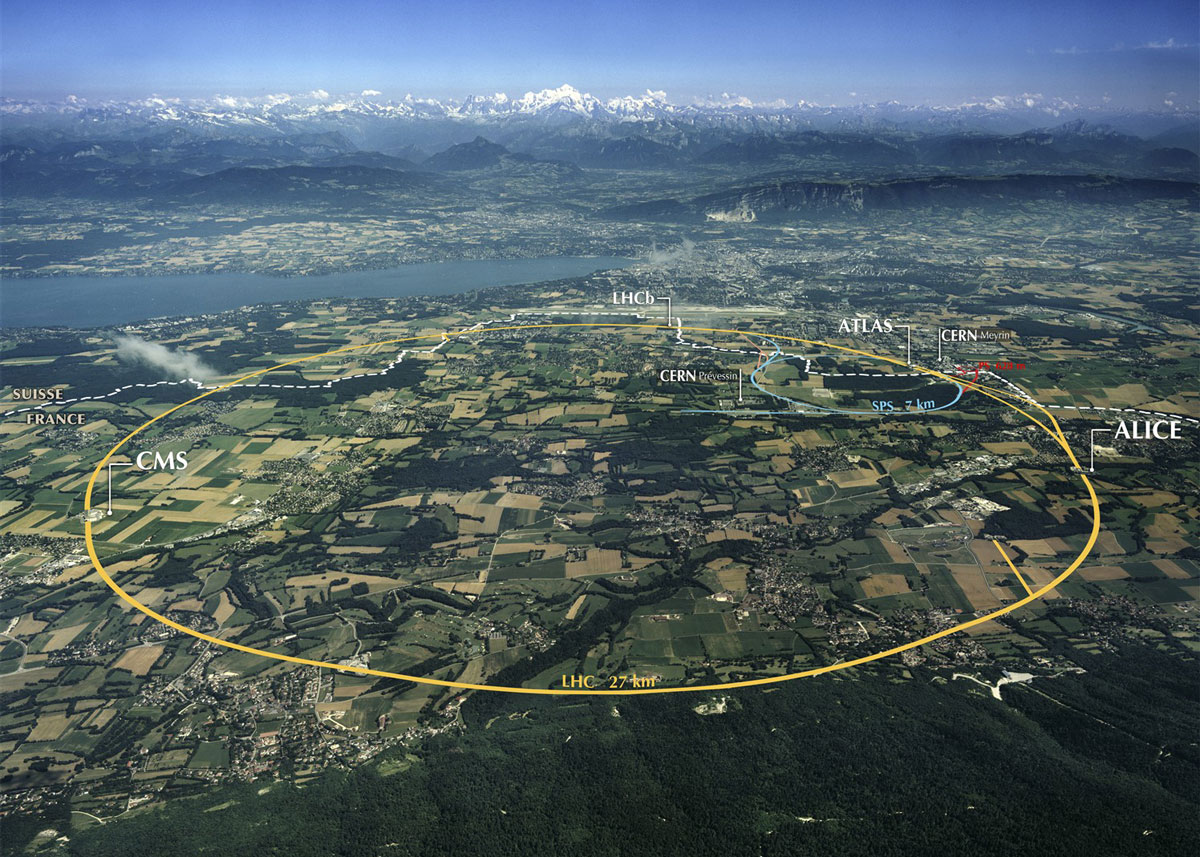
\includegraphics[width=0.8\textwidth]{cern-lhc-aerial.jpg}
\label{fig:lhc:cern-lhc-aerial}
\caption{An aerial view of Geneva, with the location of the LHC superimposed. The individual detectors (described in chapter~\ref{chapter:detector}, as well as the main CERN Meyrin site, are also highlighted. Image courtesy CERN.}
\end{figure}

%%%%%%%%%%%%%%%% 

The design of the machine aims to deliver collisions at $\sqrt{s} = 14$~\TeV~energy at a rate of $10^{34}$~\lumirate-- an energy at which protons in the LHC will be moving at 99.9999991$\%$ the speed of light, and where the beams will contain as much energy as a 38 ton truck traveling at 500 km/h.  As of 2012 collisions had only occured at 8 \TeV and a rate of $5\times10^{33}$~\lumirate-- enough to discover the Higgs Boson, but not yet enough to discover physics beyond the standard model.

The following sections describe first the history of the LHC project, followed by the details of the machine design, luminosity considerations, and operations during 2010-2012.

\section{History}
\label{lhc:history}

The LHC was first discussed publically at the ECFA-CERN Workshop held at Lausanne and Geneva in March of 1984~\cite{ECFA1984}\footnote{4 years and 1 month before the author was born!}. This was a very active time for proposing new collider experiments, as extensive work on the 40~\TeV $pp$ Superconducting Supercollider (to be built in Waxahachie, Texas) had recently displaced a proposal for a 4~\TeV~$p\bar{p}$ Dedicated Collider at Fermilab~\cite{ECFA1984,DC}, though construction continued on Fermilab's 2~\TeV~$p\bar{p}$ Tevatron collider. The Soviet Union was even planning a 6~\TeV~$p\bar{p}$ collider, the Accelerator and Storage Complex (UNK)~\cite{UNK}. In this busy landscape, the proposal of another machine at CERN-- which was currently building the Large Electron Positron (LEP), the world's largest $e^+/e^-$ collider-- was very ambitious indeed.

Several characteristics made the proposed LHC unique and worth pursuing in such a competitive environment. First, with the construction of the LEP tunnel on track for completion in 1988, the civil-engineering component of the project was greatly reduced, especially compared to the enormous expense of constructing the SSC tunnel. Second, while the design goals of 20~\TeV~collisions were at a significantly lower energy than the SSC, the projected luminosity was eventually designed to be a factor of 10 higher (10$^{34}$~\lumirate, though the initial designs focused on 10$^{33}$~\lumirate) and so the LHC could potentially gain sensitivity by accumulating data more quickly. Finally, as figure \ref{fig:lhc:lep-lhc} shows, the initial designs for the LHC invisaged the LHC beamlines actually sitting on top of the existing LEP beamlines. The resulting hybrid collider would be able to run $pp$, $ep$, and $ee$ collisions. This would not only extend the reach of the physics program by allowing for the study of deep inelastic scattering at higher energies than the HERA collider at DESY \editnote{Cite this-- HERA and $e/p$ if possible.}, but would also allow for the study of $Z$ bosons from $ee$, which could potentially be used as a calibration source for detectors before $pp$ collisions~\cite{ECFA1984}.

%%%%%%%%%%%%%%%%

\begin{figure}
\centering
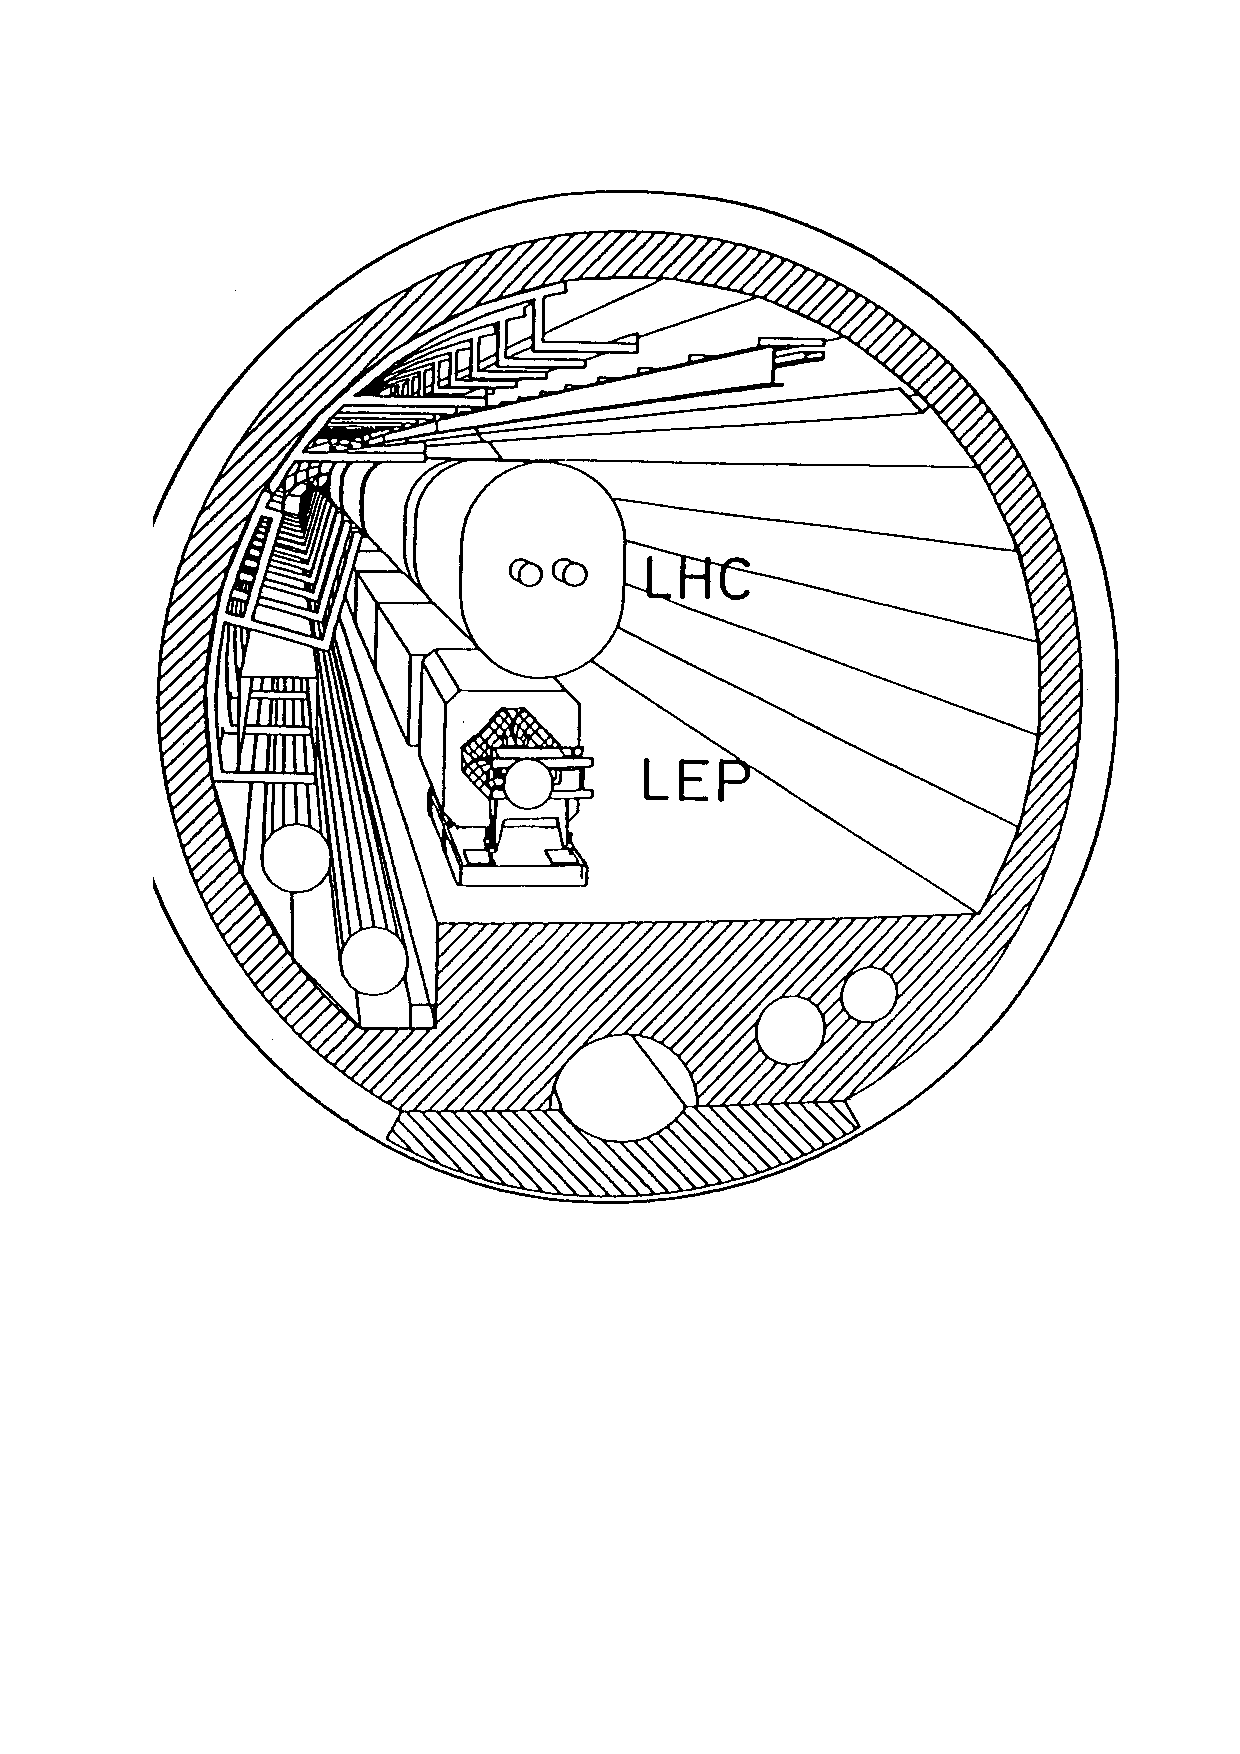
\includegraphics[width=0.8\textwidth]{lep-lhc.pdf}
\label{fig:lhc:lep-lhc}
\caption{A schematic drawing of the initial design of a shared LEP/LHC tunnel, with the LHC beamline positioned on top of the existing LEP beamline~\cite{ECFA1984}.}
\end{figure}

%%%%%%%%%%%%%%%% 

With the approval of the SSC in 1987 and the subsequent start of construction in 1991, CERN was mostly focused on the construction and operation of LEP but did not stop planning for the LHC. This proved remarkly prescient, as in the face of changing budget priorities and the end of the Cold War, the SSC was cancelled in 1993. \editnote{This probably needs citations.} CERN, on the other hand, approved a staged construction plan for the LHC in 1994, targetting first 10~\TeV~collisions in 2004 and then a higher energy in 2008.

The Conceptual Design Report~\cite{LHCCDR} published in 1995 reflected the changed landscape with the demise of the SSC and the results of more detailed cost estimates. The design energy was lowered to 14~\TeV-- higher energies would have required more costly magnets-- while the design luminosity was actually increased to 10$^{34}$~\lumirate. This increase in luminosity came at a cost: the number of interaction points was reduced to four instead of eight, and only two would receive collisions at a high rate. Critically, it was also decided to remove the LEP beamline and magnets, as it was deemed too costly to follow the existing LEP infrastructure. While this reduced the physics program of the LHC, being the only high energy hadron collider was still a rather broad portfolio. For budgetary reasons, the initial proposal was for a two-stage design, with the first stage operating with only two-thirds the dipoles and therefore a lower energy.

Non-member states joined the proposal quickly: Japan contributed in 1995; India, Russia, and Canada joined in 1996; and the US became a partner in 1997. This financial outlook for the LHC was still not completely safe, as Germany (and later the UK) unilaterally reduced their contribution to CERN between 8-9$\%$. This issue was resolved by allowing CERN to take on debt to finance the entire project in one construction phase-- a decision which raised the total cost of the LHC by $20\%$. By inviting international partners at a very early stage of the design and construction of the accelerator, CERN was able to spread costs around the world-- something that the SSC organization was not able to do, as international partnerships were not considered until too late in the construction.


With the shutdown of LEP in 2001\footnote{Not without controversy, as there was perhaps a tantalizing sign of an excess in Higgs-boson like events during the final runs of LEP.\editnote{cite me}}, the construction of the LHC began in earnest. It would take till 2007 to install the last magnet in the LHC, and the detectors finalized their own installations only in 2008. Figure~\ref{fig:lhc:lhc-tunnel} shows the final state of the LHC tunnel (without the originally planned LEP beamline). The first low-energy collisions occured on September 10, 2008, putting the LHC almost on track of its initial goal of 14~\TeV collisions in 2008. \editnote{Do I add more details on construction?}

%%%%%%%%%%%%%%%%

\begin{figure}
\centering
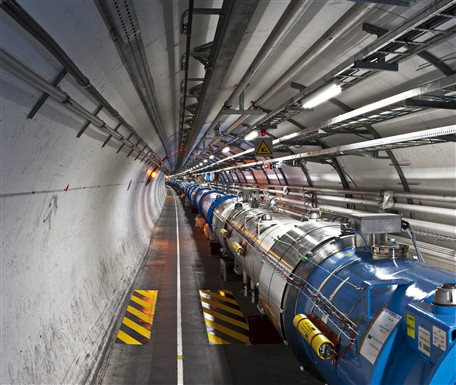
\includegraphics[width=0.8\textwidth]{lhc-tunnel.jpg}
\label{fig:lhc:lhc-tunnel}
\caption{A photo of the final LHC tunnel, no LEP beamline, in contrast to the first plans shown in Figure~\ref{fig:lhc:lep-lhc}. Photo courtesy of USLHC.}
\end{figure}

%%%%%%%%%%%%%%%% 

However, an ``incident'' on September 19 ended up delaying the full startup for a year~\cite{Incident}. On that day, the operators were testing the last sector of the LHC at current levels appropriate fo 5.5~\TeV beams. A resistive zone developed in the electrical bus connection between a dipole and quadrupole magnet. While the power supply detected this and shut down within 0.39 seconds and the quench protection circuitry began to engage at 0.89 seconds, it was already too late: an electrical arc had sparked and punctured the liquid helium enclosure and the insulation vacuum along the cryostat. This, along with the electrical noise induced by the power supply shutdown and the heat dissipation caused by the quench protection circuitry, triggered a chain reaction in which several other magnets also began to quench and other vacuum systems were degraded. As the helium began to escape the cryostat, pressure relief valves correctly opened and vented the helium to atmosphere. However, an additional complication arose: neighboring subsectors had their vacuum systems separated by vacuum barriers, meant to isolate the vacuum systems of neighboring areas. The vacuum barriers could only sustain a rather low pressure difference, and the extreme pressures generated by the evacuating helium overwhelmed these connections. The attendant large pressure forces ended up displacing dipoles from their support structures, and knocked the cryostats from their support jacks-- in some cases even ripping the anchors from the concrete floor. A total of six tons of helium, five quadrupoles, and twenty-four dipoles were lost in the incident. 

The damage to the accelerator was repaired in 2009, and on November 20, 2009, 450 GeV protons from the Super Proton Synchotron were injected into the LHC for the first time since the incident. November 23rd saw the first $pp$ collisions in all four LHC detectors, albeit at only $\sqrt{s} = 900$~\GeV. Several very short runs at this energy and $\sqrt{s} = 2.36$~\TeV followed, before the first $\sqrt{s} = 7$~\TeV collisions occured on March 30, 2010. It was decided to operate the LHC for several years at this lower energy, as more accelerator upgrades and consolidation would be required to safely operate at $\sqrt{s} = 14$~\TeV. 2010 saw a peak luminosity of only $2\times10^{32}$~\lumirate as the accelerator only very gradually increased the collision rate. 2011 saw delivery at a peak of $4 \times 10^{33}$~\lumirate-- only three times lower than the design luminosity.

After two years of successful and safe operations at the reduced energy, 2012 saw a large increase in luminosity-- to a peak of $8\times10^{33}$~\lumirate-- and an increase of the collision energy to 8~\TeV. The LHC then proceeded to shut down in 2013 until mid-2015 for a further round of repairs and consolidations of electrical connections to guarantee the safety of operations at near the design energy. As the restart of the LHC approaches in the coming months, we are anticipating collisions at 13~\TeV with luminosity likewise reaching near design levels. The LHC will have broken energy records twice in the span of five years, making this an incredibly exciting time to be working in particle physics.


\section{Machine Design}

The LHC is the last of a long chain of accelerators used to accelerate ordinary protons obtained from hydrogen gas\cite{cern-accelerators}. The entire accelerator complex is shown in Figure~\ref{fig:lhc:cern-accelerators}. Protons from a simple bottle of hydrogen gas are stripped of their electrons in an electric field and are injected into the chain at the Linac2, which accelerates the particles to 50 MeV. The Proton Synchotron Booster (PSB) then accelerates the particles to 1.4 GeV, and sends them off to the Proton Synchotron (PS) to be accelerated to 25 GeV. The Super Proton Synchotron (SPS) then accepts the protons and accelerates them to 450 GeV, which is the energy of injection at the LHC. The injection process per beam takes 260 seconds, and then another 20 minutes is required to raise the energy to collision levels.

%%%%%%%%%%%%%%%%

\begin{figure}
\centering
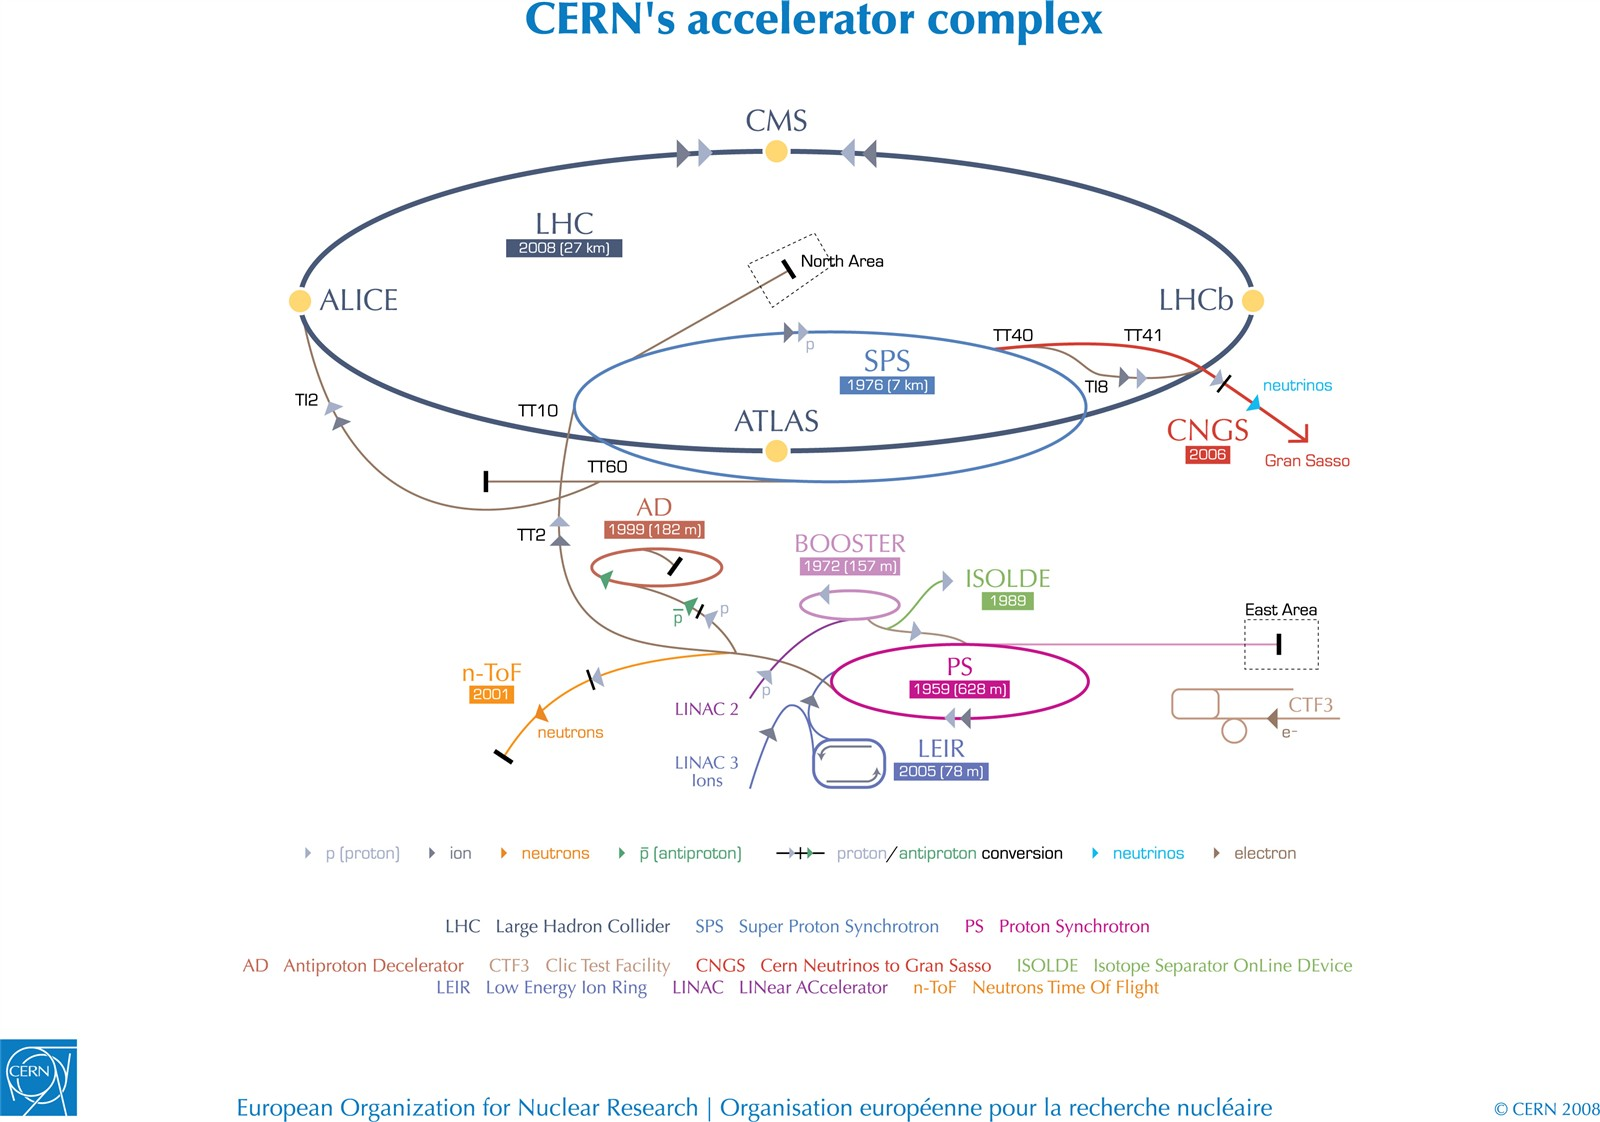
\includegraphics[width=0.8\textwidth]{cernaccelerators.jpg}
\label{fig:lhc:cern-accelerators}
\caption{A diagram of the CERN accelerator chain, with each accelerator listing both its year of completion and length. Copyright CERN.}
\end{figure}

%%%%%%%%%%%%%%%% 

Each stage of the chain accelerates particles by a factor of between 10-20 times their energy. This is a consequence of the fixed bending radius in an accelerator, $\rho$, which is~\cite{accelerator-book}:
%
\begin{equation}
\label{lhc:bending}
\frac{1}{\rho} (\mathrm{m}^{-1}) = 0.2998 \frac{|B (\mathrm{T})|}{\beta E (\GeV)}.
\end{equation}
%
As the bending radius is fixed, this means that as the energy of the beam goes up, the magnetic field must go up linearly to keep the particles inside the ring. This also means that as particles are injected from one accelerator to another (and the radius therefore increases), the magnetic field must be the same factor smaller. The lower range of practical bending magnet strength is set by stray magnetic fields in the earth; the upper range is set by the material of the magnet and energy consumption. These restrictions (how weak the magnets can be during injection, and how strong after acceleration) limit each stage of the accelerator chain to increasing the energy by a factor of $\approx$200. In practice, the accelerating factor is lower (10-20), because it is much easier to not use the full range of the magnet strength (particularly at the low end), and the size of each accelerator is not designed optimally but instead historically, as each accelerator was previously used for collisions at a lower energy. For example, the SPS could have been ejected particles at a much lower energy and the LHC accepted them by using a lower initial field strength, but as the SPS was already built, the operation of the LHC is simplified by using a higher initial field. 


The LHC itself is composed of eight essentially identical octants, as shown in Figure~\ref{fig:lhc:ring}. Octant 1 contains the collision point for ATLAS (conveniently located right next to the main CERN campus), and Octant 5 for CMS (located in the middle of the French countryside). Each octant is composed of an `insertion'-- a straight segment used for collisions, cleaning, acceleration, beam dumps, etc., as labelled in Figure~\ref{fig:lhc:ring}-- and one half of an `arc' on either end of the insertion point. Each pair of half-arcs forms a sector, which is the main organizational unit for the machine: each sector is independently powered and shares a continuous cryostat. The ring is composed of 1232 dipole magnets which bend the beam around the ring, and 852 quadruple magnets used for beam focusing. The strength of the dipole magnets limits the energy of the beam, as discussed in Equation~\ref{lhc:bending}, so these magnets are particularly critical to the machine design. They are constructed from Niobium-Titanium wire and operated at a temperature of 1.9 K (provided by superfluid helium cooling) at a strength of 8.3 T, using 11850 A of current. An additional 7000 smaller correction magnets (with sextuple, octupole, etc. configurations) are used to shape the beam. The acceleration of the beam is performed by 8 super-conducting RF cavities per beam, each providing an acceleration gradient of 5 MV/m at 400 MHz. 

Operating at full design luminosity, each beam of the LHC contains 2808 bunches each filled with $10^{11}$ protons. This corresponds to a bunch spacing of 25 ns, with longer spacing in between so-called ``bunch trains'': the exact structure of the fill pattern is determined by the fill patterns of the prior accelerators, and the need to provide gaps which can be used to safely dump the beam if necessary~\cite{lhc-bunches}\footnote{In particular, the size of these gaps is determined by the turn-on time of the LHC beam dump kicker of about 3~$\mu$s.}. In operations in 2010-2012, a minimum bunch spacing of 50 ns was used due to electron-cloud effects restricting the operation at 25 ns; the bunch charge was instead increased to deliver additional luminosity. 

Another important parameter describing the beam conditions is the \textit{emittance} $\epsilon$, defined as an ellipse with:
%
\begin{equation}
\epsilon = \gamma x^2 + 2 \alpha x x' + \beta x'^2
\end{equation}
%
where $\gamma$, $\alpha$, and $\beta$ are the ellipse parameters, and $x$ is a coordinate and $x'$ the velocity of that coordinate~\cite{accelerator-book}. The overall emmittance $\epsilon$ is conserved by Liouville's theorem, but focusing magnets can change the other parameters of the ellipse. In particular, as $\beta$ shrinks and $\gamma$ grows, the physical size of the beam in that direction becomes smaller, but with a wider range of velocities. Thus at interaction points, $\beta$ is minimized such that the transverse size of the two beams are minimized and collisions are most likely. This particular value is called $\beta^*$, and is a key parameter in describing the luminosity of the accelerator. Note that in principle each transverse coordinate can have indepedent sizes, but typically circular beams are assumed.

%%%%%%%%%%%%%%%%

\begin{figure}
\centering
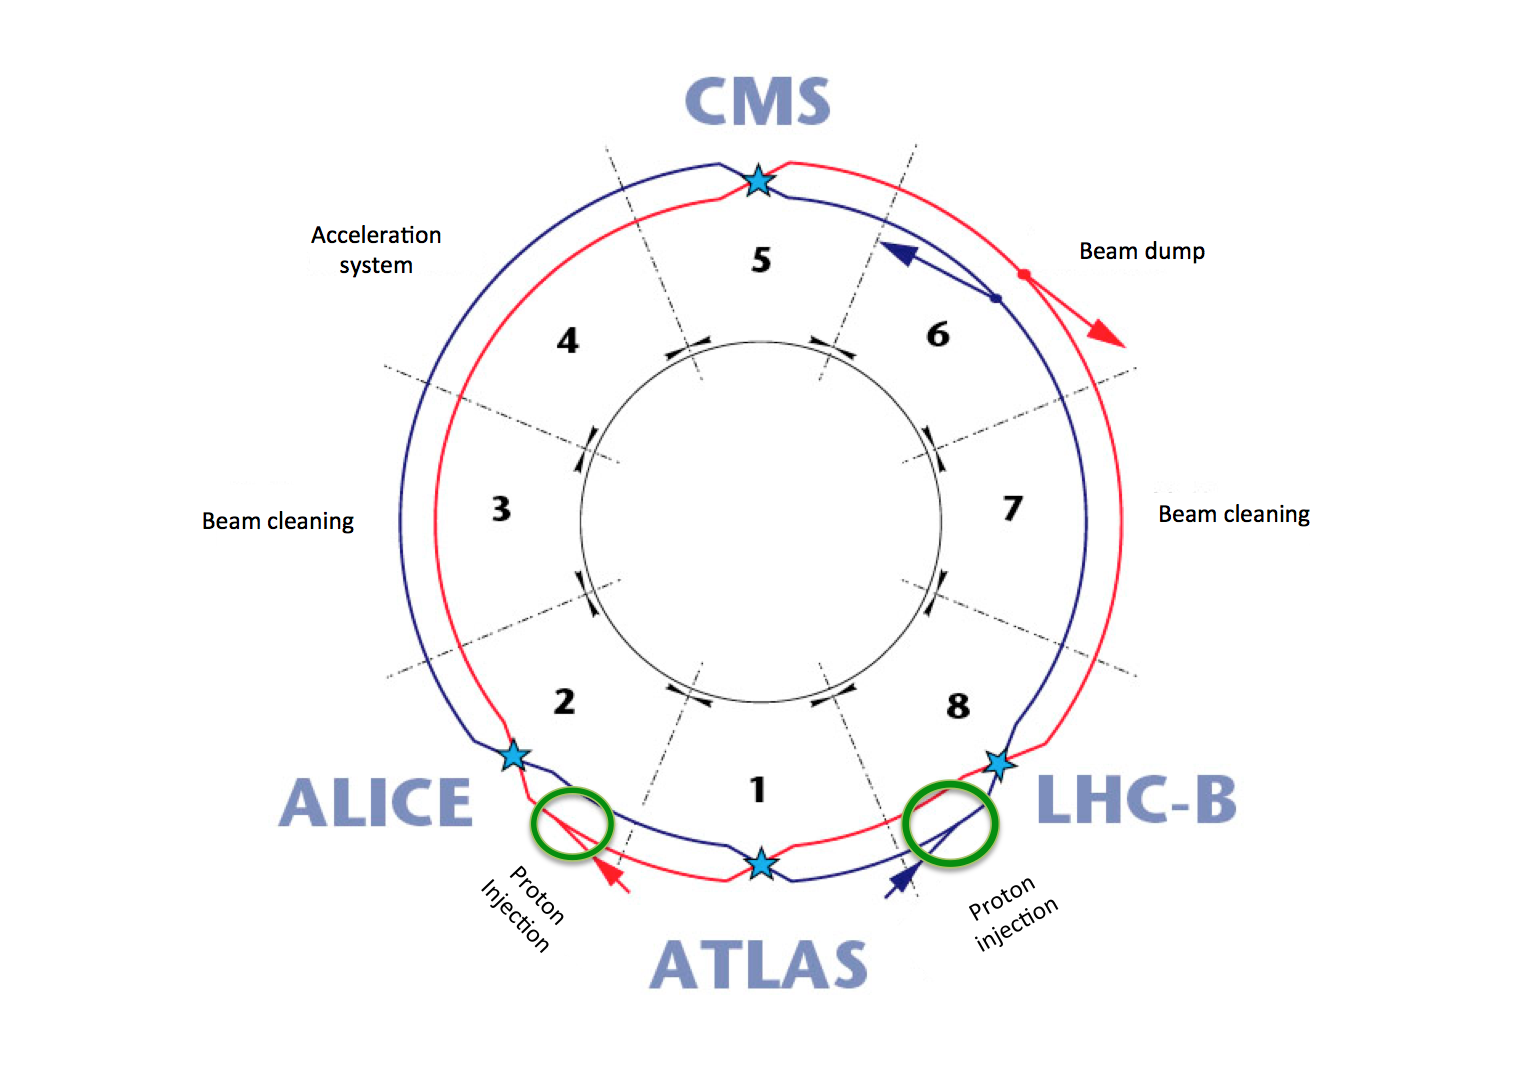
\includegraphics[width=0.8\textwidth]{ring.png}
\label{fig:lhc:ring}
\caption{A diagram of the CERN accelerator chain, with each accelerator listing both its year of completion and length. Copyright CERN.}
\end{figure}

%%%%%%%%%%%%%%%% 

\section{Luminosity, and Pileup}
\label{lhc:luminosity-and-pileup}

Assuming the beams are circular, all of the previously discussed beam parameters come together in defining the luminosity:
%
\begin{equation}
\mathcal{L} = \frac{N^2 k_b f \gamma}{4\pi \epsilon_n \beta^*} F
\end{equation}
%
where $N$ is the number of protons per bunch, $k_b$ is the number of bunches per beam, $f$ is the revolution frequency, $\gamma$ is the relativistic factor, $\epsilon_n$ is the normalized emittance, $\beta^*$ is the $\beta$ value at the IP, and $F$ is a geometric factor indicating the crossing angle of the beams. This shows clearly the handles that the accelerator operators have to increase the luminosity: they can increase the number of protons and the number of bunches, or decrease the size of the beam.

Luminosity is a measurement of the rate of collisions; the \textit{integrated luminosity} refers to the amount of data collected over a period of time. Luminosity is typically reported in units of \lumirate, which is an inverse cross-section per time. Another commonly used unit is the \textit{barn}, which is $10^{-24}$ cm$^2$. Luminosities in ATLAS are typically reported in \ipb~or \ifb. The product of the integrated luminosity and the cross-section of production for some physics process ($pp \rightarrow t\bar{t}$, $pp \rightarrow \tilde{g}\tilde{g}$, etc.) gives the number of events expected for that process in that amount of data.

Increasing the number of bunches (which is possible by switching from 50 ns bunchspacing to 25 ns, for example) increases the frequency of bunch crossings, but does not increase the rate of collisions per bunch crossing. The other factors do the opposite: they keep the rate of bunch crossings constant, but increase the rate of collisions per bunch crossing. Historically in hadron colliders, the expected number of collisions per crossing has been very low, and often less than 1. With the extremely strong performance of the LHC, however, the rate of collisions per crossing has increased to significantly more than one, leading to the condition of \textit{pileup}.

As the expected rate of bunch-crossings is 400 MHz-- far higher than what the detectors can record-- a triggering system is typically used to quickly identify ``interesting'' events for read-out and future analysis. The rate of interesting events is much lower than that of the full interaction cross-section, so there is typically only one interesting event per bunch crossing (at most). This means that when an interesting event is recorded, it is embedded in a background of other collisions, which is the pileup. The LHC is the first collider which has to deal with significant levels of pileup, as it was not feasible to use an even lower bunch-spacing, leaving only increasing the per-bunch collision rate to increase the overall luminosity.

The pileup profiles-- defined using the variable $\mu$, or the average number of collisions per bunch-crossing-- for 2011 and 2012 operations is shown in Figure~\ref{fig:lhc:mu-profile}. $\mu$ is an average variable which describes the beam conditions-- the actual number of interactions per bunch-crossing can fluctuate with Poisson statistics, and is better measured with variables like $N_{vtx}$, the number of reconstructed primary vertices using the tracking detectors. The wide distribution of $\mu$ values is due to two effects. First, the operation of the accelerator is optimized throughout the year, leading to lower values of $\beta^*$ and higher $N$ and $k_b$, and thus changing $\mu$ over time. Additionally, the expected $\mu$ can change during a run-- in particular, as collisions occur and the number of protons in a bunch decreases over time, $\mu$ will decrease proportionally.

%%%%%%%%%%%%%%%%

\begin{figure}
\centering
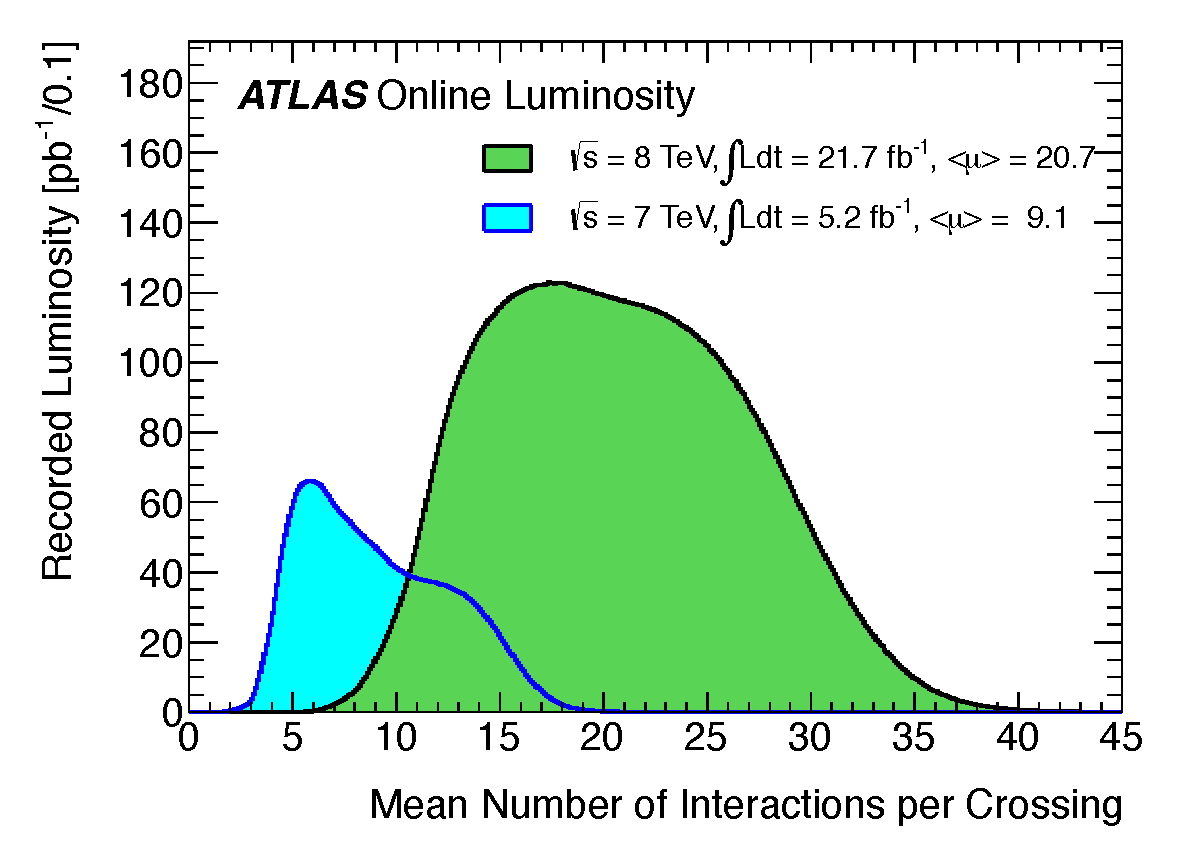
\includegraphics[width=0.7\textwidth]{mu_2011_2012-dec.pdf}
\label{fig:lhc:mu-profile}
\caption{The profile of the average number of interactions per bunch crossing, $\mu$, delivered during operations in 2011 and 2012.}
\end{figure}

%%%%%%%%%%%%%%%% 


\section{Operations in 2010-2012}

Operations during Run 1 of the LHC were extraordinarly successful: in 2010, the collider delivered 48.1 \ipb to ATLAS, 5.46 \ifb in 2011, and 22.8 \ifb in 2012. Figure~\ref{fig:lhc:lumivsyear} shows the integrated luminosity delivered as a function of time, demonstrating the remarkable advances in collision rate as accelerator operations became more advanced. Table~\ref{tab:lhc:parameters} shows the typical beam parameters in each year of operation, compared to the design. In some respects-- emittance and proton number-- the LHC is actually outperforming the design specifications, which has led to very high luminosity levels even with a 50 ns bunch spacing. This comes at the price of the much higher than expected pileup levels, and the correponding difficulties in detector operation that this creates.

%%%%%%%%%%%%%%%%

\begin{figure}
\centering
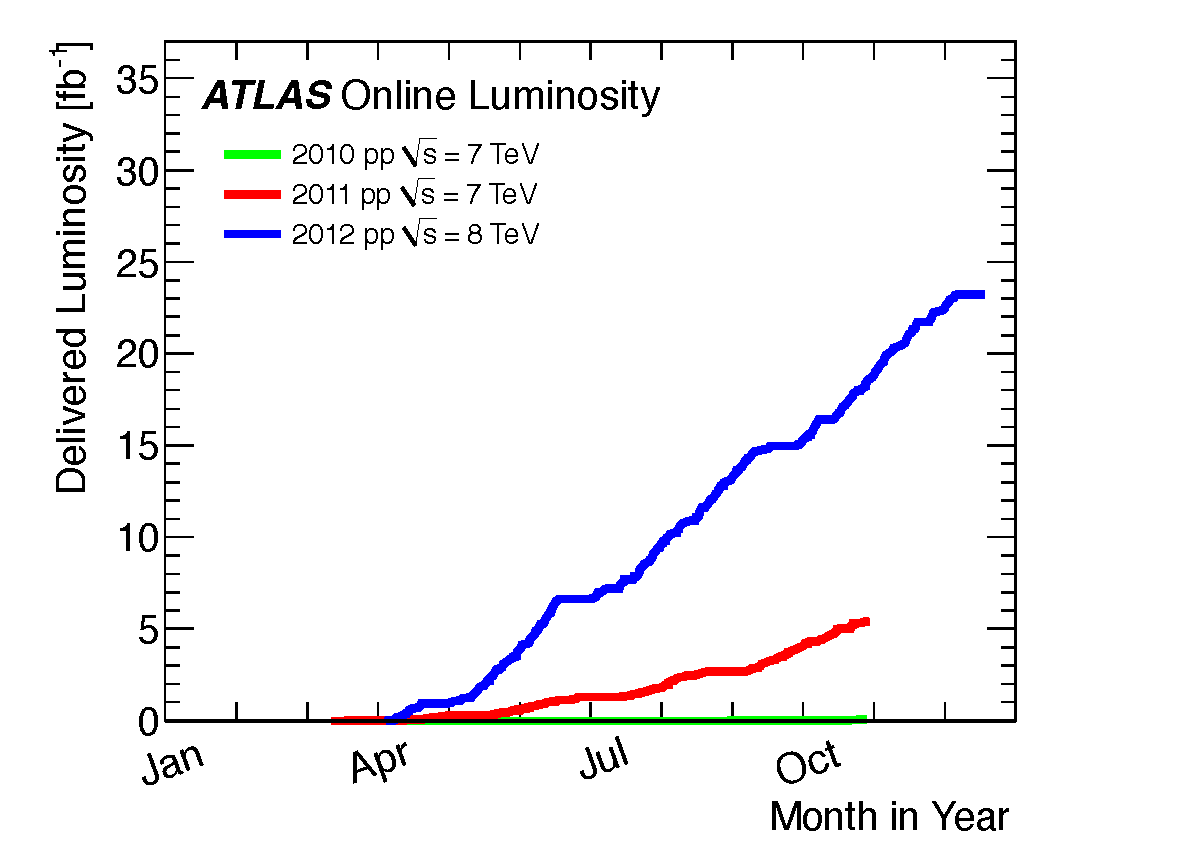
\includegraphics[width=0.7\textwidth]{intlumivsyear.pdf}
\label{fig:lhc:lumivsyear}
\caption{The integrated luminosity as a function of time in Run 1, as measured by the ATLAS detector.}
\end{figure}

%%%%%%%%%%%%%%%% 

\begin{table}
	\caption{Table of LHC run parameters in Run 1, and the design.}
	\label{tab:lhc:parameters}
	\begin{center}
		\begin{tabular}{l|cccc}
		\hline

		\hline
		\textbf{Parameter} & \textbf{2010} & \textbf{2011} & \textbf{2012} & \textbf{Design} \\
		\hline
			 Beam Energy [TeV] & 3.5 &        3.5    &       4.0 &            7.0\\
			 $\beta^*$ [m]      & 2.0/3.5 &     1.5/1.0   &       0.6 &            0.55\\
			 Bunch spacing [ns] & 150 &         75/50   &       50 &             25\\
			 Number of bunches  & 368 &         1380    &       1374 &           2808\\
			 Average proton number  & 1.2 $\times 10^{11}$ &    1.45 $\times 10^{11}$     3.5    &   1.7 $\times 10^{11}$ &     1.15 $\times 10^{11}$\\
			 Normalized emittance at start of fill [mm.mrad]  & 2.0 &    2.4 &      2.5    &   3.75\\
			 Peak luminosity [\lumirate] & $2.1\times 10^{32}$   &  $3.7 \times 10^{33}$   & $7.7 \times 10^{33}$ & $1 \times 10^{34}$ \\
			 Maximum $\mu$ &  4  &  17   &  40 & 19 \\
		\hline

		\hline
		\end{tabular}
	\end{center}
\end{table}

Figure~\ref{fig:lhc:lumivstime} shows the peak luminosity as a function of time in Run 1, and Figure~\ref{fig:lhc:muvstime} shows the peak pileup rate during the same period. In particular, it is clear that the growth is directly related: almost the entirety of the luminosity gain seen in 2011 and 2012 came at the price of increased pileup.

%%%%%%%%%%%%%%%%

\begin{figure}
\centering
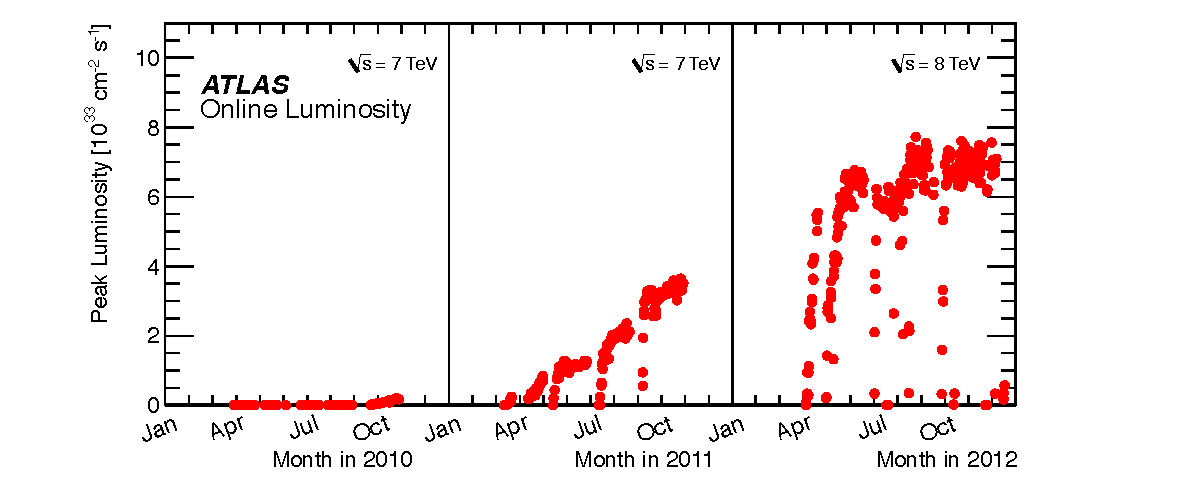
\includegraphics[width=0.7\textwidth]{lumivstime.pdf}
\label{fig:lhc:lumivstime}
\caption{Peak luminosity delivered by the LHC as a function of time in Run 1, as measured by the ATLAS detector.}
\end{figure}

%%%%%%%%%%%%%%%% 


%%%%%%%%%%%%%%%%

\begin{figure}
\centering
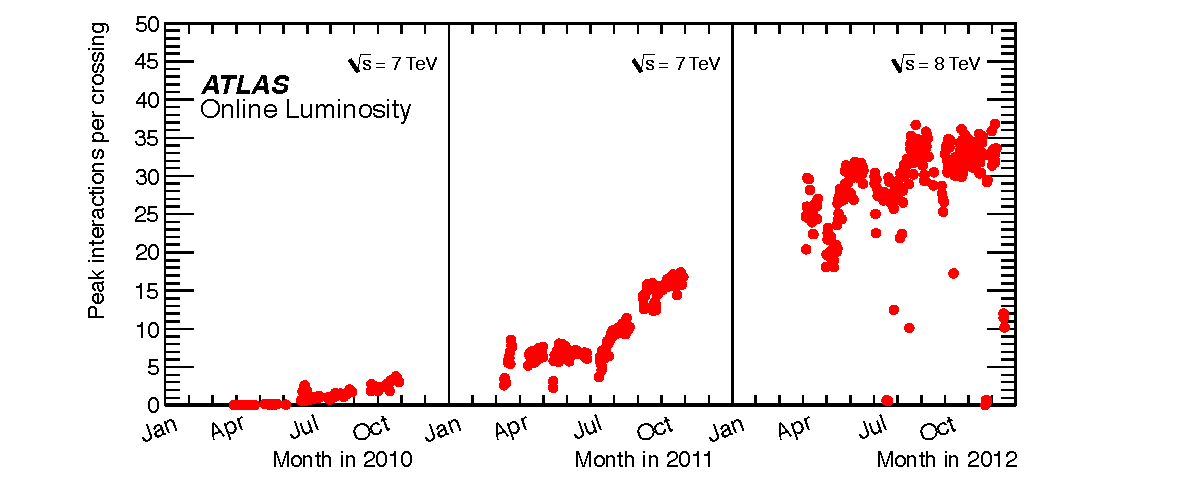
\includegraphics[width=0.7\textwidth]{muvstime.pdf}
\label{fig:lhc:muvstime}
\caption{Peak interactions per crossing as a function of time in Run 1, as measured by the ATLAS detector.}
\end{figure}

%%%%%%%%%%%%%%%% 



		

\chapter{The ATLAS Detector}
%!TEX root = ../swiatlow_thesis.tex
\label{chapter:detector}

The design of the LHC, with two high-luminosity interaction points at opposite ends of the ring, called for two general purpose detectors to be built in these locations. Their charge was to accurately reconstruct collision events in the most hostile conditions yet seen in a collider: with a bunch spacing of 25 ns and the unprecedented introduction of pile-up the detectors would have an enormous challenge ahead of them in dealing with both the rate and the reconstruction of events. ATLAS (A Toroidal LHC APparatus)~\cite{ATLASPaper} and CMS (Compact Muon Solenoid)~\cite{CMSPaper} were the two detectors built for this task, with ATLAS occupying the (much more convenient) Point 1 and CMS located at the (very distant) Point 5. The data presented in this thesis was collected by the ATLAS experiment in $pp$ collisions at $\sqrt{s} = 8$~TeV in 2012. 

Particle detectors measure particles via their interactions with matter, as drawn schematically in Figure~\ref{fig:detector:schematic}. For example, charged particles (such as electrons and some hadrons) interact electromagnetically with silicon and gas tubes, leaving hits in different layers of detectors which can be traced back to form a track. Electrons and photons, with their low masses and high rate of interaction with matter, are measured by the electromagnetic calorimeter. The calorimeter is composed of alternating layers of metal meant to cause the particle to interact and lose energy, and active materials which measure the energy left behind in these interactions. The hadron calorimeter follows a similar principle, and alternately placed layers of metal and active material again aim to stop and measure the hadrons which the electromagnetic calorimeter did not stop. Muons, which do not interact very much with matter most matter but do leave hits in trackers, survive past even the hadronic calorimeter, and a special set of muon detectors can be used to identify them there. Neutrinos, as they interact with matter only via the weak force and thus very rarely, escape detection and are reconstructed only by inferring their presence from the lack of momentum conservation in the transverse plane.

A significant constraint in the design of detectors is the interaction of particles with matter. \editnote{This needs citations.} As particles traverse matter-- including the detectors built to measure them-- they lose energy via interactions, or in the case of photons, can even convert into electron/positron pairs. As some detectors-- particularly the calorimeters-- sit radially behind others, this can mean that substantial portions of the energy of particles can have already dispersed by the time they are measured. One of the keys to an accurate detector, then, is to minimize the material before the calorimeters. \editnote{Clean this up with better discussion of radiation lengths. Pages 350 of Perkins may be helpful}


%%%%%%%%%%%%%%%%

\begin{figure}
\centering
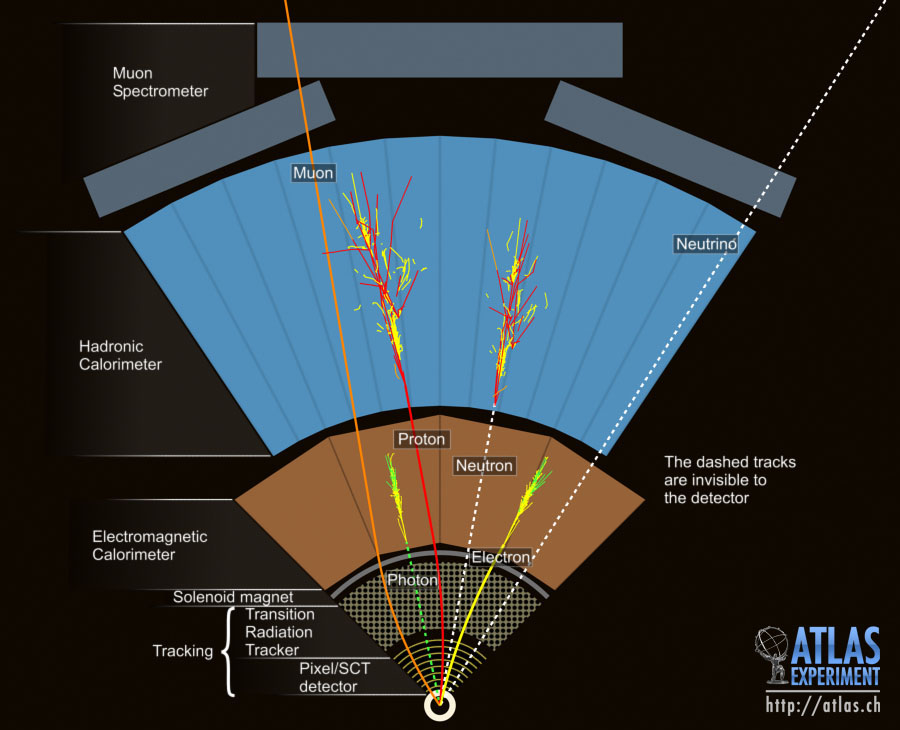
\includegraphics[width=0.7\textwidth]{schematic.jpg}
\label{fig:detector:schematic}
\caption{A schematic diagram of the interactions of various particles with detector components. Copyright CERN.}
\end{figure}

%%%%%%%%%%%%%%%% 

General purpose particle detectors thus demand the following characteristics: \editnote{define radiation lengths? above?}

\begin{enumerate}
	\item Tracking systems must be able to identify primary and secondary vertices, while minimizing the radiation lengths before the calorimeters
	\item Strong calorimetry systems are required to accurately measure the energy and position electrons, photons, and hadrons
	\item Muon systems must be able to precisely reconstruct muons
	\item All detector systems must be capable of being read out quickly, and a triggering system is required to quickly identify interesting events for recording
\end{enumerate}

To this end, the ATLAS detector is built in the traditional onion-layer configuration, which measures particles as they travel perpendicular to the beam~\cite{ATLASPaper}. The Inner Detector, composed of the concentric Pixel, SCT \editnote{define}, and Transition-Radiation-Tracker (TRT) subsystems, lies at the center of the detector and precisely measures tracks created by charged particles. A 2 T solenoid encloses the Inner Detector, bending charged particles and enabling the measurement of their momenta. Next the Electromagnetic Calorimeter (ECal), composed of liquid argon (LAr) and copper, sits outside of the solenoid in a liquid nitrogen cryostat, and measures energy deposits from electrons and photons (as well as hadrons to a lesser extent). The Hadronic Calorimeter, built to measure and stop any remaining hadronic particles, is composed of steel and scintillating tile in the center (referred to as the barrel), and LAr and copper in forward regions (referred to as end-caps). Surrounding these are an additional set of magnets: the superconducting air-core toroids of the barrel and endcaps, which bend particles in the plane perpendicular to that of the bending due to the solenoid. \editnote{That needs cleaning.} The Muon Spectrometer (composed of MDT, RPC, TGC, and CSC subsystems) sits outside of (and next to) these magnets, and provides a final measurement of the charged particles which reach that far. The entire detector is shown in Figure~\ref{fig:detector:atlas}. The incredible size of the detector-- 25 m in diameter, and 46 m long-- is dominated by the Muon Spectrometer and the toroids. On the other hand, the detector is comparatively light (only 7000 tons, compared to 14,000 tons for CMS), as the air-core toroids do not add substantial weight to the detector~\cite{CMSPaper,ATLASPaper}.


%%%%%%%%%%%%%%%%

\begin{figure}
\centering
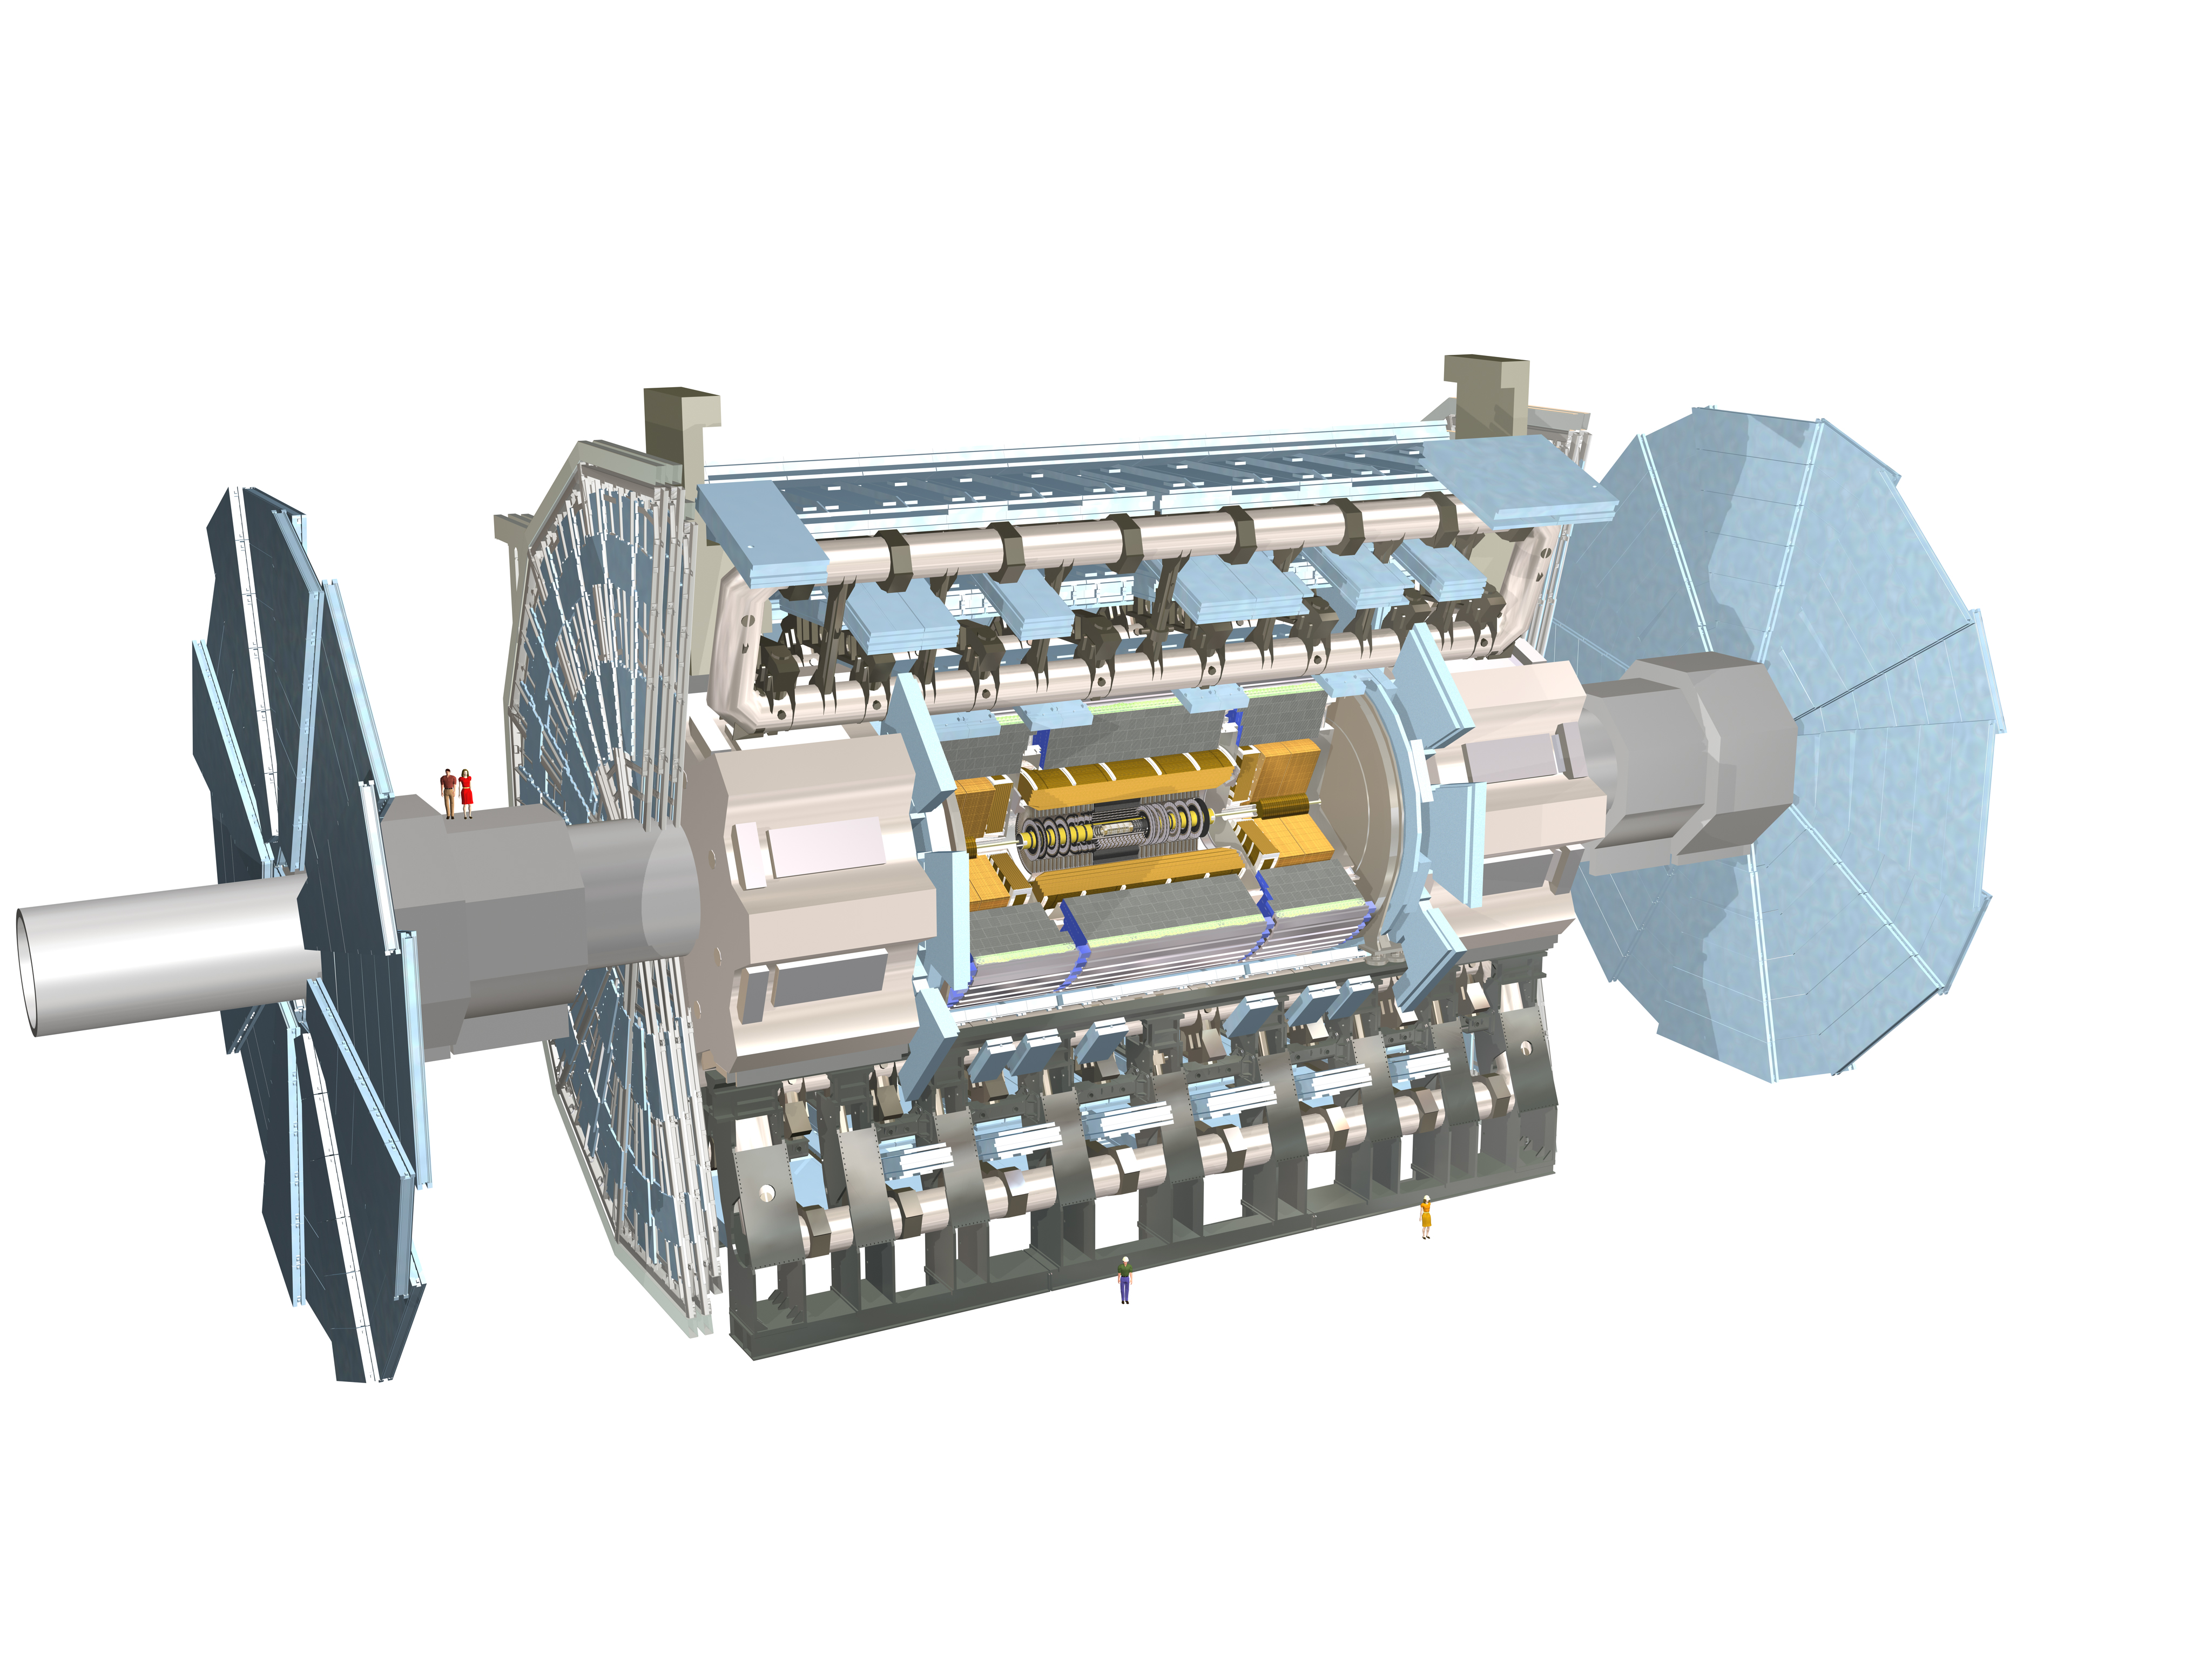
\includegraphics[width=0.85\textwidth]{atlas.jpg}
\label{fig:detector:atlas}
\caption{A computer-generated view of the ATLAS detector, with people for scale. Copyright CERN.}
\end{figure}

%%%%%%%%%%%%%%%% 


In keeping with the principle of ``similar, but opposite'' established by their locations, the ATLAS and CMS detectors take complementary approaches to the various aspects of event reconstruction in collisions. All general purpose detectors have the same basic goals: the must reconstruct the outgoing, stable particles produced in collisions and the subsequent decays of particles in these collisions. Different particles are detected with different general classes of detectors, of which there are many possible types. For example, electrons and photons are measured by the ECal, for which ATLAS used a liquid argon (LAr) and copper system while CMS used a crystal lead tungstate system. Each had their own advantages and disadvantages (ATLAS's was less costly and already proven technology with better position resolution, while CMS took a riskier route which promised better energy resolution), but overall performance between the detectors tends to be very similar because of various trade-offs. In the case of the ECals, the precision of ATLAS and CMS's $H\rightarrow \gamma \gamma$ measurements ended up being largely similar \editnote{cite?}, in no small part because CMS's all-silicon tracking system introduced greater radiation lengths before the calorimeters, thereby prompting more photons to convert and losing precision in the measurement. On the other hand, CMS's comparatively weak brass hadronic calorimeter (compared to ATLAS's higher resolution tile calorimeter), is compensated by their tracking system, which enables a particle-flow reconstruction algorithm to combine information from all detectors and improve jet performance to levels very similar to ATLAS. \editnote{consider citations, and substantial revisions here}. Similarly, the large size and extra toroid magnets of ATLAS allow for a larger lever-arm and an additional set of measurements of muons (enabling reconstruction with or without the inner detector): however, muon reconstruction performance in CMS is very similar because the stronger solenoidal magnetic field (4 T compared to 2 T) allows for a better measurement using the inner detector only (with the muon systems on CMS providing only a tag of a passing muon, and not a complete reconstruction). 


%2012 luminosity figure? Or in LHC section?



%Detector figure

\section{History}

The first public discussion of the proposals which became the ATLAS detector occurred in 1992 at the General Meeting on LHC Physics at Evian-les-Bains~\cite{Evian,EvianCourier}. At the time, four general purpose detectors (much like the four detector configuration in place at LEP) were seriously considered: EAGLE, ASCOT, CMS, and L3 (as an upgrade to the existing LEP detector, including a movable stage which would allow it to take data from both $e^+/e^-$ and $pp$ collisions). Several additional single purpose (heavy ion, neutrino, and $B$-physics) detectors were also proposed.

ATLAS emerged in a later 1992 Letter of Intent as a merger of the ASCOT and EAGLE collaborations~\cite{ATLAS-LoI}. ASCOT (Apparatus with SuperCOnducting Toroids) contributed the physically-defining feature of the secondary toroidal magnet system and standalone muon measurement system, as well as the tradition of using a tortured amalgamation of letters to form a name. EAGLE (Experiment for Accurate Gamma, Lepton and Energy measurements) on the other hand featured a stronger 2 T magnetic field, and inner-detector and calorimeter designs more similar to some of the final ATLAS systems. The detector described in the Letter of Intent already resembled ATLAS in many important ways, featuring the superconducting air-core toroids, accordion-shaped liquid Argon electromagnetic calorimeters, scintillating tile hadron calorimeters, and multi-design inner detector. \ref{fig:detector:earlyatlas} shows an early drawing of ATLAS from the Letter, and already the detector looks recognizable to its current form.

% Any citations on UA1 origins?

%%%%%%%%%%%%%%%%

\begin{figure}
\centering
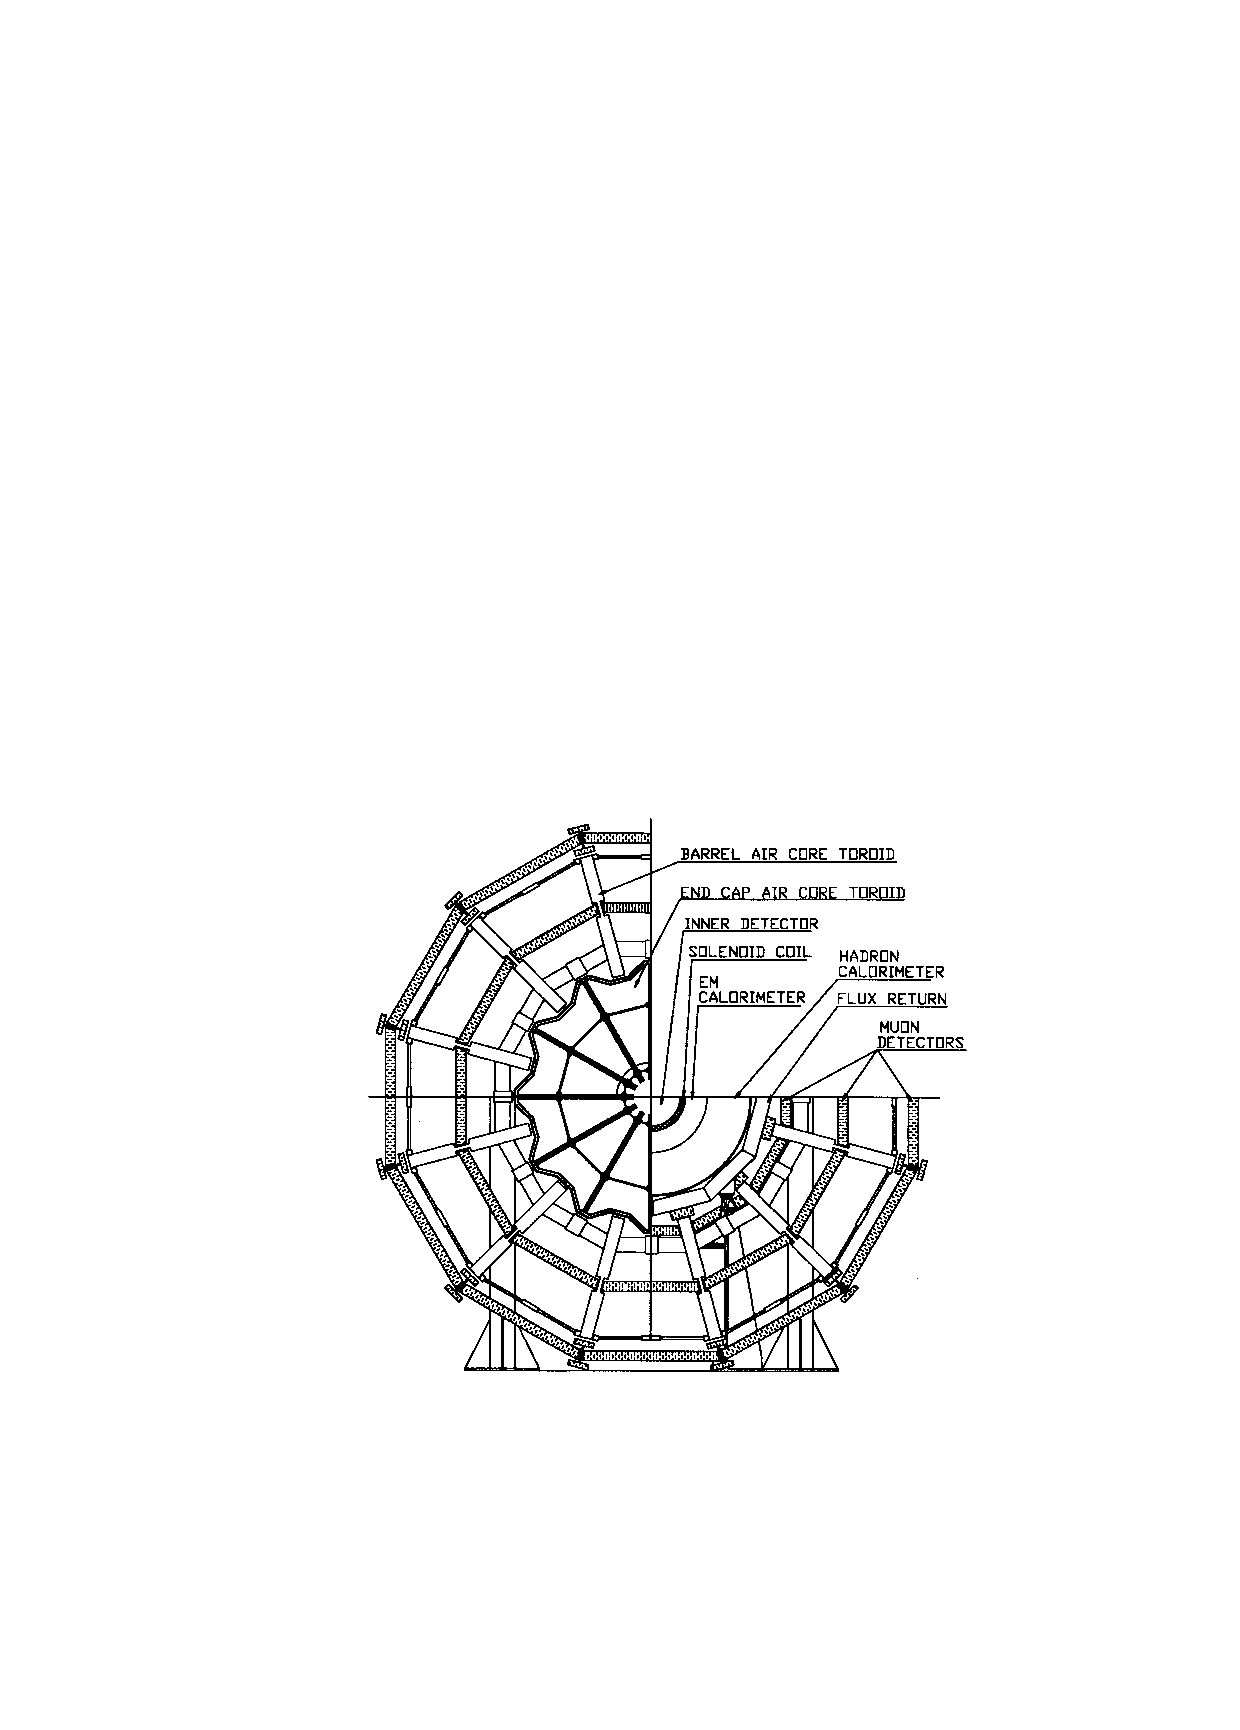
\includegraphics[width=0.7\textwidth]{early-atlas.pdf}
\label{fig:detector:earlyatlas}
\caption{An early view of a potential superconducting air-core toroid magnet system for the ATLAS detector from the 1992 Letter of Intent~\cite{ATLAS-LoI}.}
\end{figure}

%%%%%%%%%%%%%%%% 

By the release of the 1994 Technical Proposal~\cite{ATLASTP}, the detector design was becoming much more complete, and many of the choices of design for the detector subsystems (the components of the ID, for example) were already mostly complete. By 1997 many of the detector subsystem Technical Design Reports (TDR) were complete, and construction began on these systems~\cite{ATLASHistory}. 1999 saw a TDR for the entire detector, representing a complete integrated design for the entire detector~\cite{tdr1,tdr2}. Memoranda of Understanding with national funding institutions are completely arranged by 2000, as construction of the detector is well underway~\cite{ATLASHistory}. The cavern, the largest yet built at CERN and pictured in Figure~\ref{fig:detector:cavern}, is completed in 2003. Assembly of detector components continues rapidly at this point, and the detector is finished in 2008.

%%%%%%%%%%%%%%%%

\begin{figure}
\centering
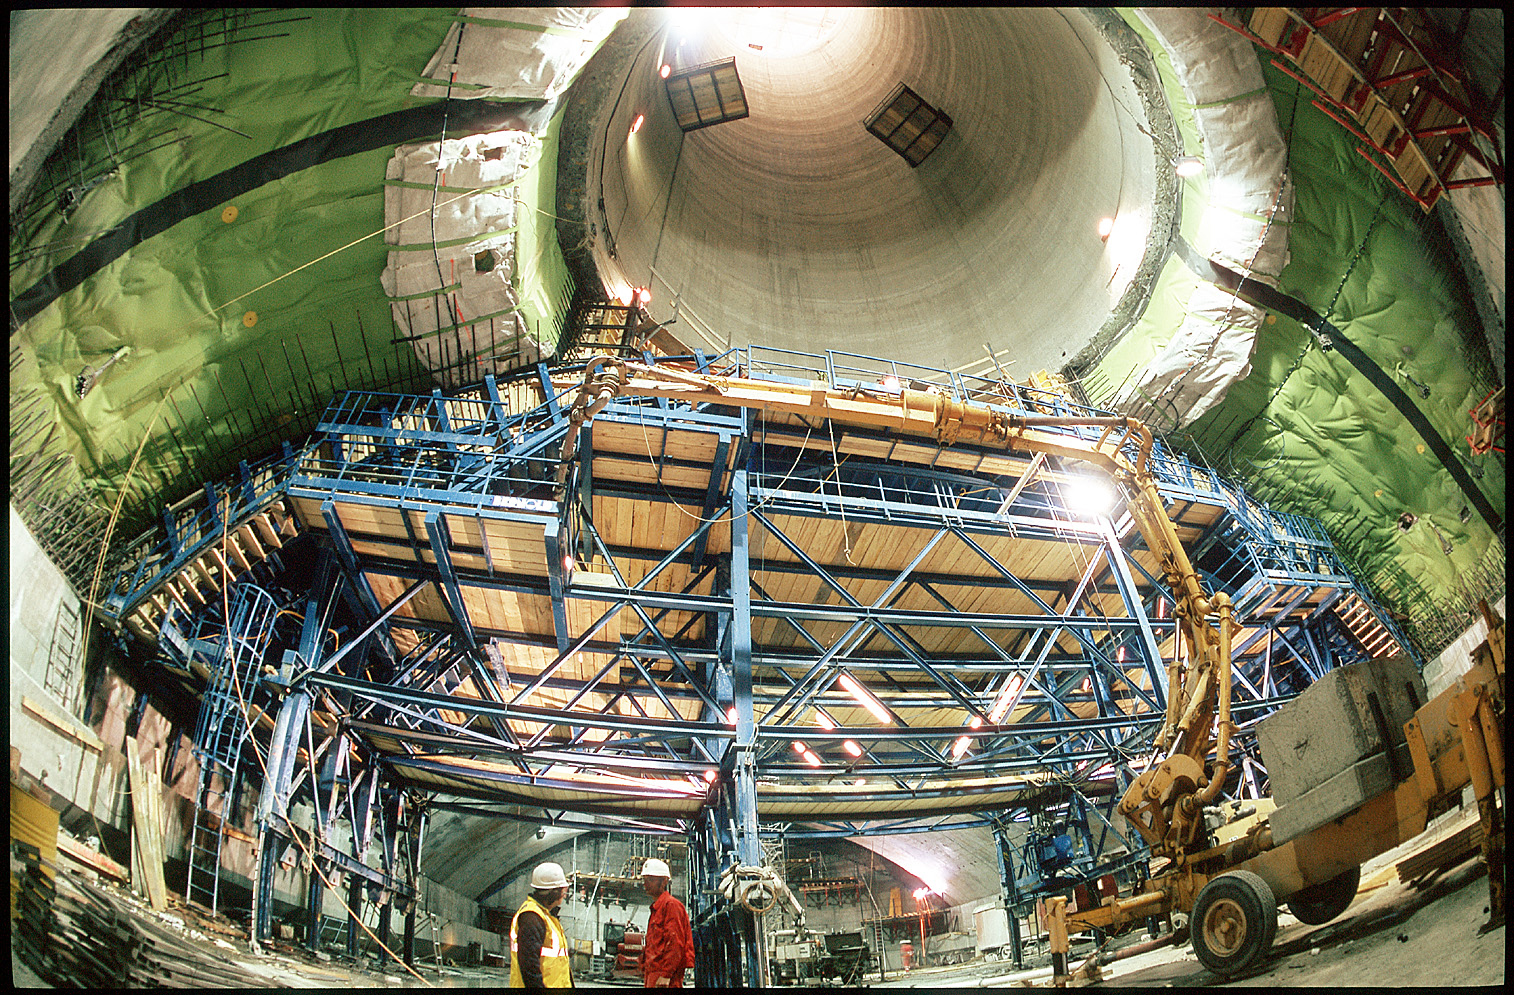
\includegraphics[width=0.7\textwidth]{cavern.jpg}
\label{fig:detector:cavern}
\caption{A view of the ATLAS cavern during construction. Copyright CERN.}
\end{figure}

%%%%%%%%%%%%%%%% 

Early data-taking was of course disrupted by the incident described in Section~\ref{lhc:history}, and first 7 TeV collisions were recorded on March 3, 2010. ATLAS recorded 35 \ipb~in 2010, 4.6 \ifb~in 2011, and 20.3 \ifb~in 2012. The dramatic increase of data during 2011 and 2012 came at the cost of pileup levels far higher than what had been planned for. As Section~\ref{atlas:data-quality} describes, the detector operated incredibly well during these difficult conditions, and over 90\% of data delivered by the LHC was successfully recorded.





% approval dates

% cavern construction (picture?)

% construction milestones

% first data, first papers

% quenching? higgs discovery


\section{Magnet Systems}

The magnets of ATLAS play a critical role in the meausurement of particle momenta by bending charged particles via the interaction with the Lorentz Force Law:

\begin{equation}
\frac{d \vec{p}}{d t} = q (\vec{E} + \vec{v} \times \vec{B})
\end{equation}
%
where $\vec{p}$ is the particle 4-momentum, $q$ is the charge, $v$ is the velocity, and $E$ and $B$ are the electric and magnetic fields. The solenoid, for example, has a field in $z$ direction only, resulting in a force in the $\phi$ direction. As the magnetic field does no work, the energy of the particle is not changed, and only the direction is affected. The degree of bending is directly proportional to $\vec{v}$, the velocity, and so the particle's momentum is able to be extracted. The field configuration in the toroid systems is much more complicated, but the particle momentum reconstruction follows the same general principle. \editnote{Clean this up, and cite.}

The combined magnet system is shown in Figure~\ref{fig:detector:magnets}. The solenoid sits at the center, and the toroid system on the outside and in the endcaps.

%%%%%%%%%%%%%%%%

\begin{figure}
\centering
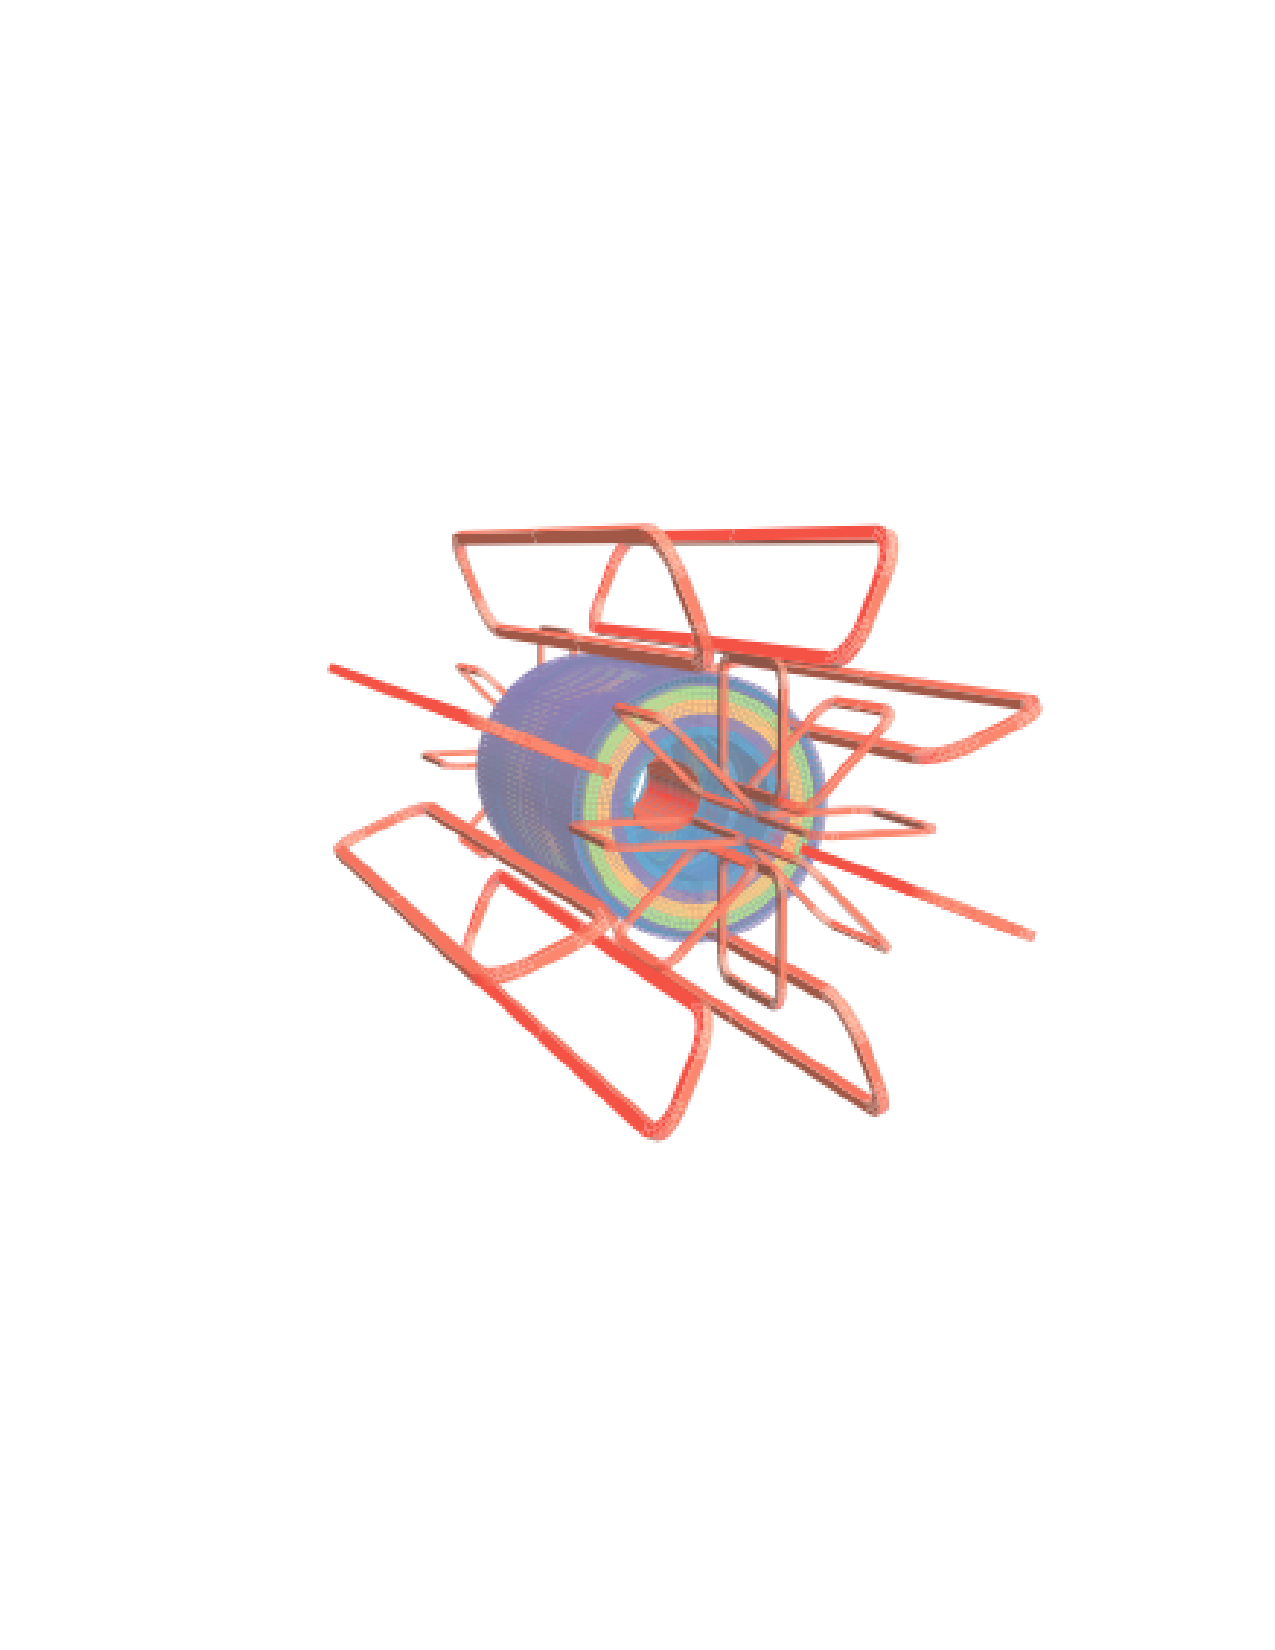
\includegraphics[width=0.7\textwidth]{magnet-fields.pdf}
\label{fig:detector:magnets}
\caption{A computer generated visualization of the ATLAS magnet systems.}
\end{figure}

%%%%%%%%%%%%%%%% 


\subsection{Solenoid}
\label{atlas:magnets:solenoid}

ATLAS's solenoid is shown in Figure~\ref{fig:detector:solenoid} shortly after its construction was finished. It sits inside the calorimeter systems, and surrounds the Inner Detector. This is contrast to the configuration in CMS, where their solenoid surrounds the calorimeter systems. Thus, particles in ATLAS do not bend in the calorimeters and particle showers tend to be more directly collimated, while particles tend to be dispersed much further in the calorimeter in CMS.

The ATLAS solenoid has a 2 T axial field, powered by 7.730 kA of current~\cite{ATLASPaper}. Since the solenoid is in front of the calorimeters, care must be taken to reduce the material that particles can interact with. To that end, the magnet and the LAr calorimeter share the same vacuum vessel, eliminating the need for two additional walls. The magnet is composed of Al-stabilized NbTi conductor, developed specifically to best balance high field and low thickness. The solenoid occupies the space between 2.46 and 2.56 m, and is 5.8 m long axially. The stored energy of the magnet system is approximately 40 MJ, and it takes approximately a week to cool the magnet to the operational temperature of 4.5 K. 

%%%%%%%%%%%%%%%%

\begin{figure}
\centering
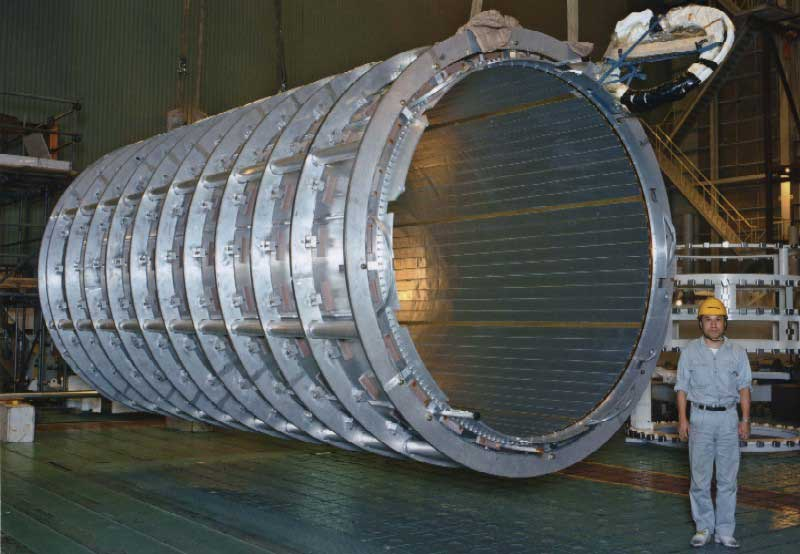
\includegraphics[width=0.7\textwidth]{solenoid.jpg}
\label{fig:detector:solenoid}
\caption{A photograph of the ATLAS solenoid shortly after the winding of the coils was finished. Copyright CERN.}
\end{figure}

%%%%%%%%%%%%%%%% 


\subsection{Barrel toroids}

The ATLAS magnet system contains two separate toroids systems~\cite{ATLASPaper}. The barrel toroid consists of 8 coils in separate racetrack-configured, stainless-steel vacuum vessels which give the ATLAS the detector its famous shape, as seen in Figure~\ref{fig:detector:toroid}. The magnets are supported by a system of 8 inner and 8 outer support rings. The entire system is 25.3 m long, and begins at 9.4 m radially and ends at 20.1 m. The magnet is composed of the same wire as used in the solenoid, and the magnet system stores 1.1 GJ of energy during operation at 20.5 kA of current. The barrel toroid takes approximately 5 weeks to cool to its nominal temperature of 4.6 K.


%%%%%%%%%%%%%%%%

\begin{figure}
\centering
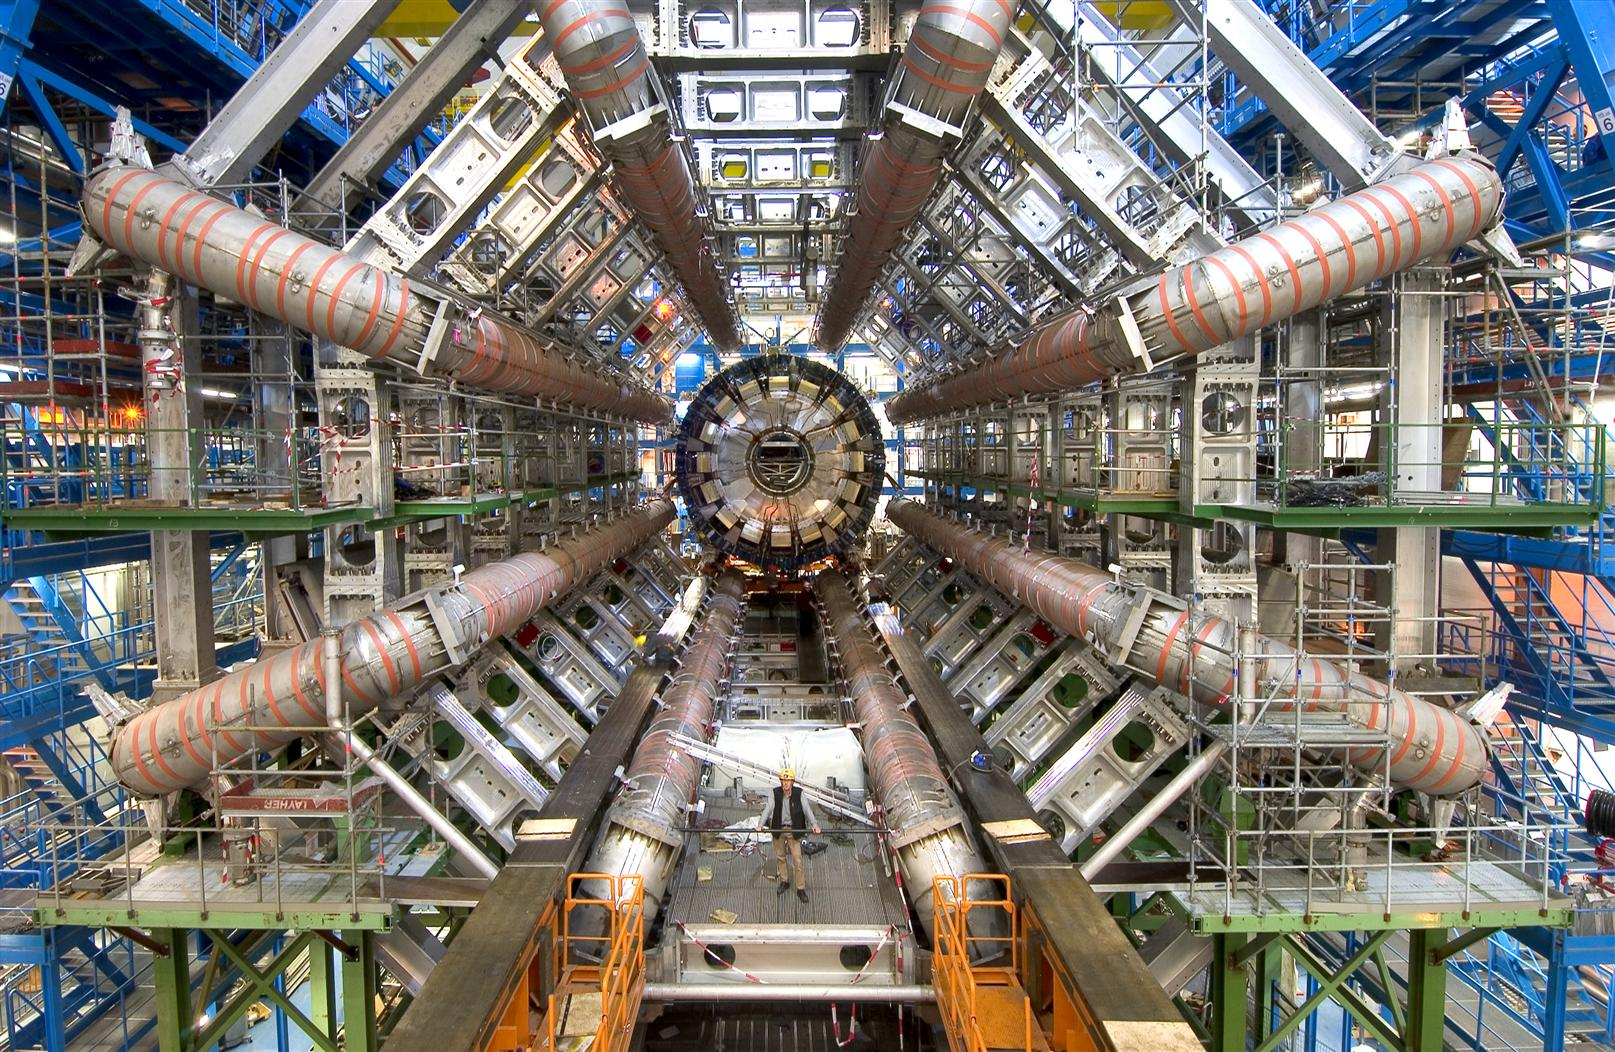
\includegraphics[width=0.7\textwidth]{toroid.jpg}
\label{fig:detector:toroid}
\caption{A photograph of the ATLAS barrel toroids after their installation. Note person in the center for scale. Copyright CERN.}
\end{figure}

%%%%%%%%%%%%%%%% 

\subsection{Endcap toroids}

The third ATLAS magnet system are the endcap toroids~\cite{ATLASPaper}. These magnets are designed bend the muons which interact with the muon spectrometer endcaps. They are constructed to be removable in order to allow access to the calorimeter and inner detector systems. The endcaps are each constructed of 8 flat, square coils with 8 keystone wedges which share the same cryostat. The magnets each take four weeks to cool to the operating temperature of 4.5 K, and operate at 20.5 kA with a stored energy of 0.25 MJ each. The coil material is again largely similar to that of the barrel toroid and solenoid. One of the endcap toroids is pictured in Figure~\ref{fig:detector:endcap-toroid} after being lowered into the ATLAS cavern.


%%%%%%%%%%%%%%%%

\begin{figure}
\centering
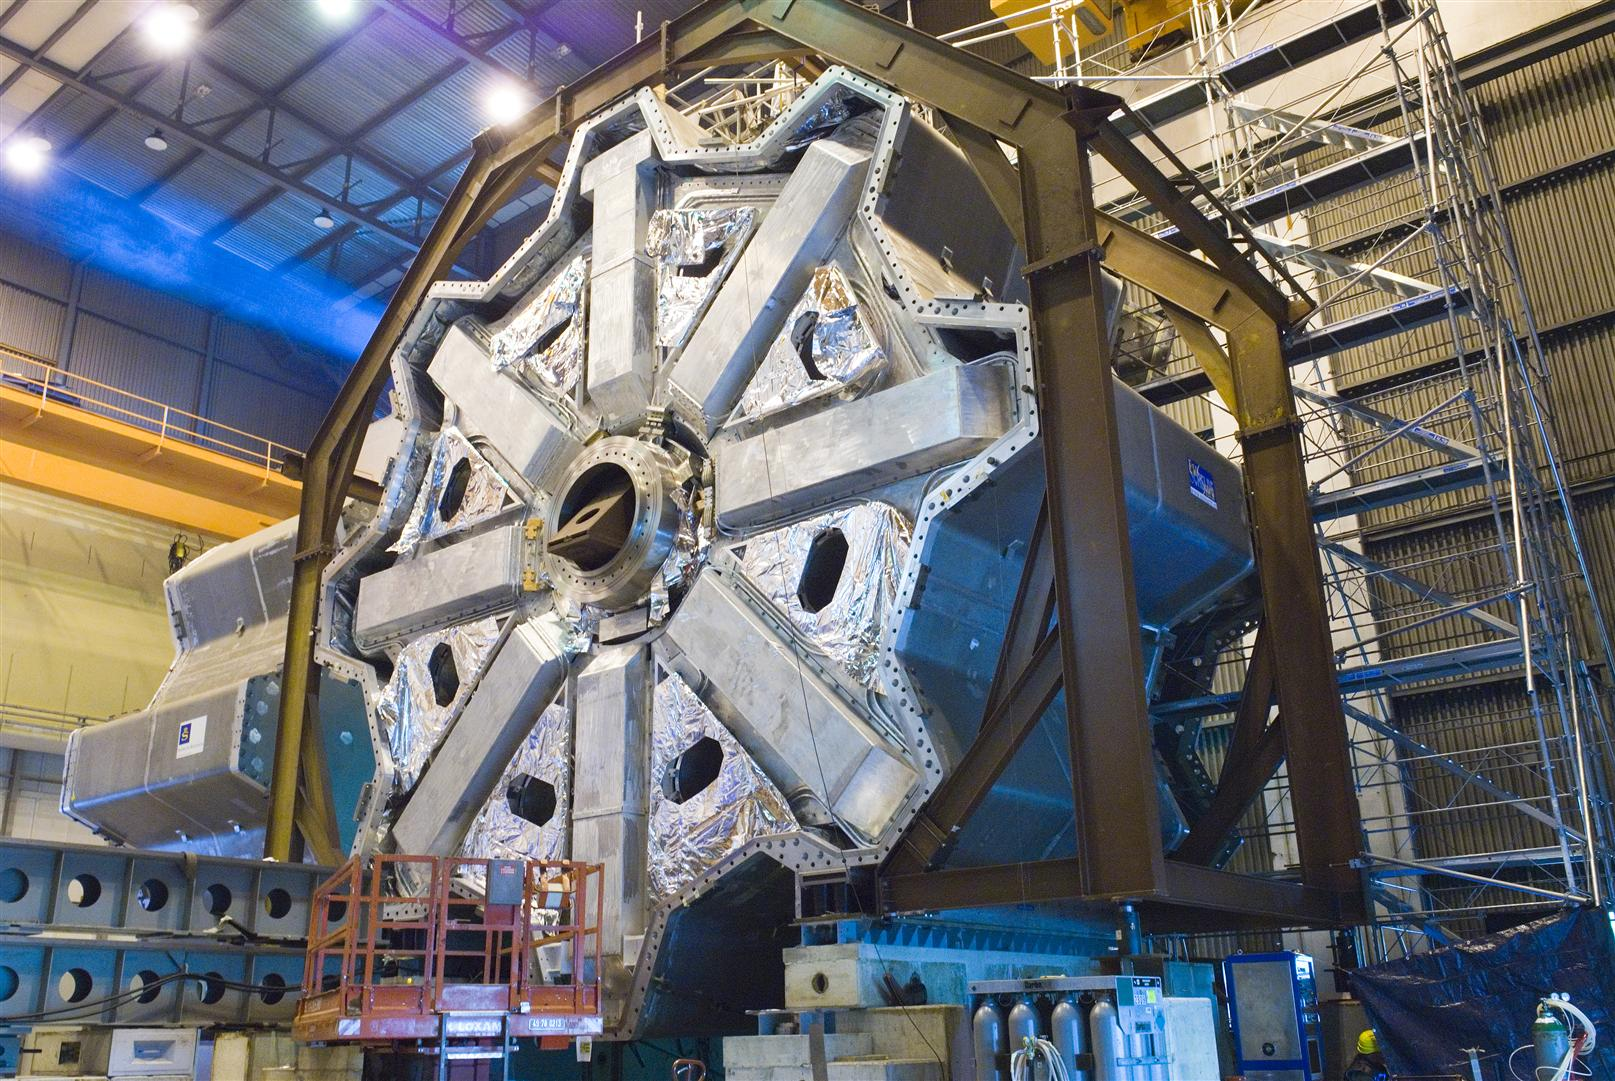
\includegraphics[width=0.7\textwidth]{endcap-toroid.jpg}
\label{fig:detector:endcap-toroid}
\caption{A photograph of an ATLAS endcap toroid shortly before its installation in the detector. Copyright CERN.}
\end{figure}

%%%%%%%%%%%%%%%% 


\section{Inner Detector}

The ATLAS Inner Detector (ID) sits at the center of the experiment~\cite{ATLASPaper}. The purpose of the detector is to reconstruct the tracks (i.e. trajectories) of charged particles produced by the collisions of the LHC in order to not only accurately measure the locations of primary and secondary vertices, but to also directly measure the momenta and locations of charged particles~\cite{ATLASExpected}. The detector covers the range $|\eta| < 2.5$, and is capable of measuring particle momenta as low as $\pT = 500$~MeV. Charged particle reconstruction efficiencies are typically greater than $90\%$ for 100 GeV particles and $70\%$ for 1 GeV particles, with a strong $\eta$ dependence. Typical \pT resolutions are of order $0.05\% \mathrm{GeV}^{-1} \times \pT \oplus 1\%$, and impact parameter resolutions are approximately 10 $\mu$m\footnote{The impact parameter is the perpendicular distance from the origin to the point of closest approach of the track, and is critical for the measurement of secondary vertices.}. 

The ID is composed of several independent detector subsystem which read out the locations of interactions with charged particles. These hits are fit to tracks by a suite of tools, which include standard global-$\chi^2$ and Kalman-filters, but also several specialized fitters~\cite{ATLASExpected}. The \pT of the particles is obtained by measuring the curvature produced by the 2 T solenoid (as described by Section~\ref{atlas:magnets:solenoid}) surrounding the detector. The three subsystems, described below, are the silicon pixel tracker (Pixel), silicon microstrip tracker (SCT), and transition radiation tracker (TRT). The combined detector has a length of 7024 m and a radius of 1.15 m~\cite{ATLASPaper}. Figure~\ref{fig:detector:inner-detector} shows a computer generated image of the combined ID, and Figure~\ref{fig:detector:inner-detector-2} shows a computer-generated image of the various subcomponents of the ID and their spacing. Figure~\ref{fig:detector:inner-detector-3} shows the $\eta$ range of the various detector subsystems, displaying the transition between barrel and endcap components.

At design luminosity, the detector is expected to measure approximately 1000 charged particles every 25 ns within the detector acceptance~\cite{ATLASExpected}. The added growth of pileup in the 2012 and future LHC runs have increased the importance of the Inner Detector as the primary vertex identification has become even more critical~\cite{ATLAS-CONF-2012-042}, but growing challenges from the computing time necessary to fit so many tracks (which increase more than quadratically as the number of detector hits~\cite{Combinatorics}) will also need to be overcome to make best use of the detector's information.

%%%%%%%%%%%%%%%%

\begin{figure}
\centering
\includegraphics[width=0.7\textwidth]{inner-detector.jpg}
\label{fig:detector:inner-detector}
\caption{A computer-generated view of the ATLAS inner detector, with relevant sizes of the detector marked out. Copyright CERN.}
\end{figure}

%%%%%%%%%%%%%%%% 

%%%%%%%%%%%%%%%%

\begin{figure}
\centering
\includegraphics[width=0.7\textwidth]{inner-detector-2.jpg}
\label{fig:detector:inner-detector-2}
\caption{A cut-out view of the ATLAS inner detector, showing the layers a particle would interact with as it passed outward from the collision point. Copyright CERN.}
\end{figure}

%%%%%%%%%%%%%%%% 

%%%%%%%%%%%%%%%%

\begin{figure}
\centering
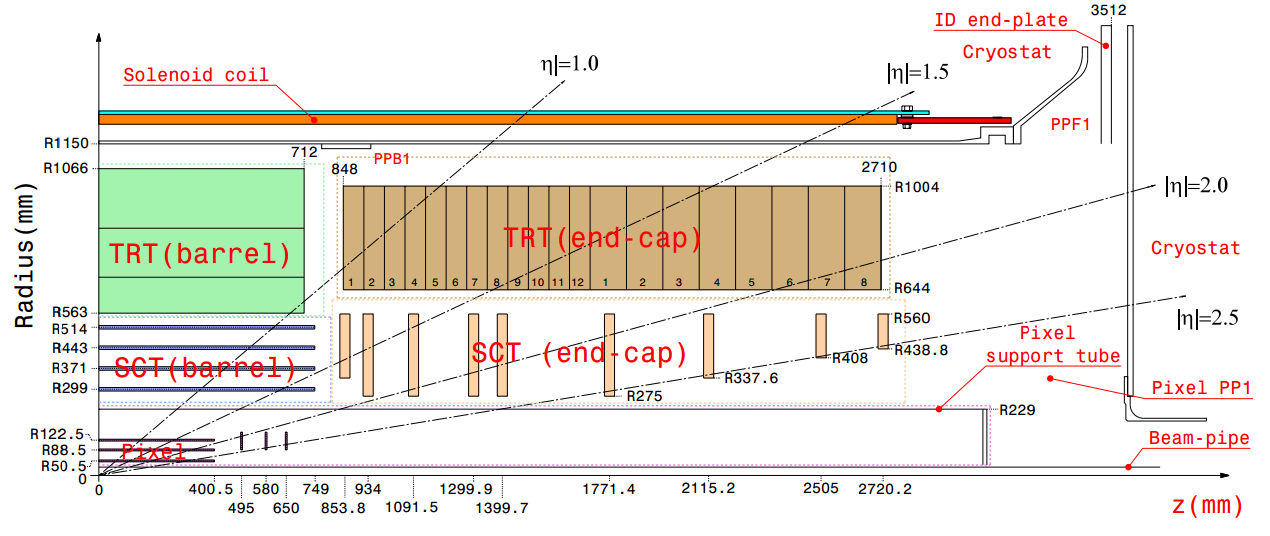
\includegraphics[width=0.7\textwidth]{tracker-eta.png}
\label{fig:detector:inner-detector-3}
\caption{A cut-out view of the Inner Detector and the locations in $r$, $z$ (with lines of detector $\eta$ demarcated) of the various detector subsystems.}
\end{figure}

%%%%%%%%%%%%%%%% 


\subsection{Silicon Pixel Detector}

The innermost ATLAS sub-detector is the Silicon Pixel Detector~\cite{Pixel,ATLASPaper}. The principal of detection for the pixel detector follows the standard ionizing radiation detector~\cite{Detectors}. Charged particles interact with the active medium (doped silicon), knocking electrons loose from their host atoms and creating electron-hole pairs. An applied voltage carries the holes and electrons to opposite ends of the detectors, where they are read out. The active regions are very small in both $x$ and $y$ dimensions, allowing for many independent measurement channels in a small area. Given the high number of particles expected from LHC collisions, and that the density is greatest nearest to the interaction point, it is critical that the innermost detector have a huge number of very small channels, making the task perfectly suited for a pixel detector.

80.4 million independent pixel channels, with a size of $50 \times 400~\mu$m, are read out by 1744 bump-bonded modules attached to the active sensors. Each of the modules are composed of 16 radiation hard front-end chips~\cite{ATLASPaper}. This corresponds to a combined active area of 1.7 $m^2$. The detector is arranged in three radial layers in the barrel section, and three disks in the end-caps. In the radial layers, the pixels have a resolution of $10 \times 115~\mu$m in $R-\phi$ and $z$ respectively, and in the end-caps the orientation is perpendicular and the resolution is $10 \times 115~\mu$m in $R$ and $R-\phi$: the orientations are always chosen such that the most precise measurement takes place in the direction most relevant to the measurement of the track $p_T$.\footnote{The $R-\phi$ coordinate is simply a distance-projected version of the azimuthal angle $\phi$.} The barrel and disk arrangement is shown in Figure~\ref{fig:detector:pixel}. Hits are read out when charge has been collected over a tunable threshold determined by the noise of each pixel, resulting in typical occupancies of $10^{-4}$ -- $10^{-5}$, though this grows obviously grows with additional $pp$ interactions.

The innermost radial layer, known as the $b$-layer, sits only 50.5 mm from the center of the beampipe, while the outermost layer is located at 122.5 mm~\cite{ATLASPaper}. By placing detectors so close to the interaction point, it is possible to very accurately measure the location of both  primary vertices-- the locations of $pp$ collisions-- and second vertices-- the locations of the displaced decays of particles with long lifetimes, such as $B$-hadrons~\cite{ATLASExpected}.

Placing the detector so close to the beamline comes at a price, however, as the detector is particularly susceptible to radiation damage due to the high flux of particles through a small area. At design luminosity, this is expected to be about 158 kGy/year at the $b$-layer, reduced to 25.4 kGy/year at the outermost layer~\cite{ATLASPaper}. Damage comes in the form of displaced atoms in the doped silicon lattice, resulting in lower electron-hole yields per particle interaction. Some of the damage is mitigated by operating at cold temperatures (typically $-5$ to $-10$\degree~C), and higher bias voltages can also alleviate the effects.

While the entire Inner Detector is expected to be replaced after 300 \ifb~are collected in order to replace the damaged components, the long shutdown of 2013-2015 presented ATLAS with the opportunity to augment the existing pixel detector with the so-called Insertable B-Layer (or IBL)~\cite{ATLASIBL}. The IBL, which adds an additional layer of pixels to the barrel and endcap pixel systems, is attached directly to a new carbon-fiber beampipe, and is located only 33 mm from the center of the beampipe. Due to this extremely close distance, the pixel size has been further reduced to $50 \times 250 \mu$m. The vertexing performance (especially secondary vertex identification for $b$-tagging) of ATLAS in Run 2, starting in 2015, is expected to substantially increase due to the IBL. 

%%%%%%%%%%%%%%%%

\begin{figure}
\centering
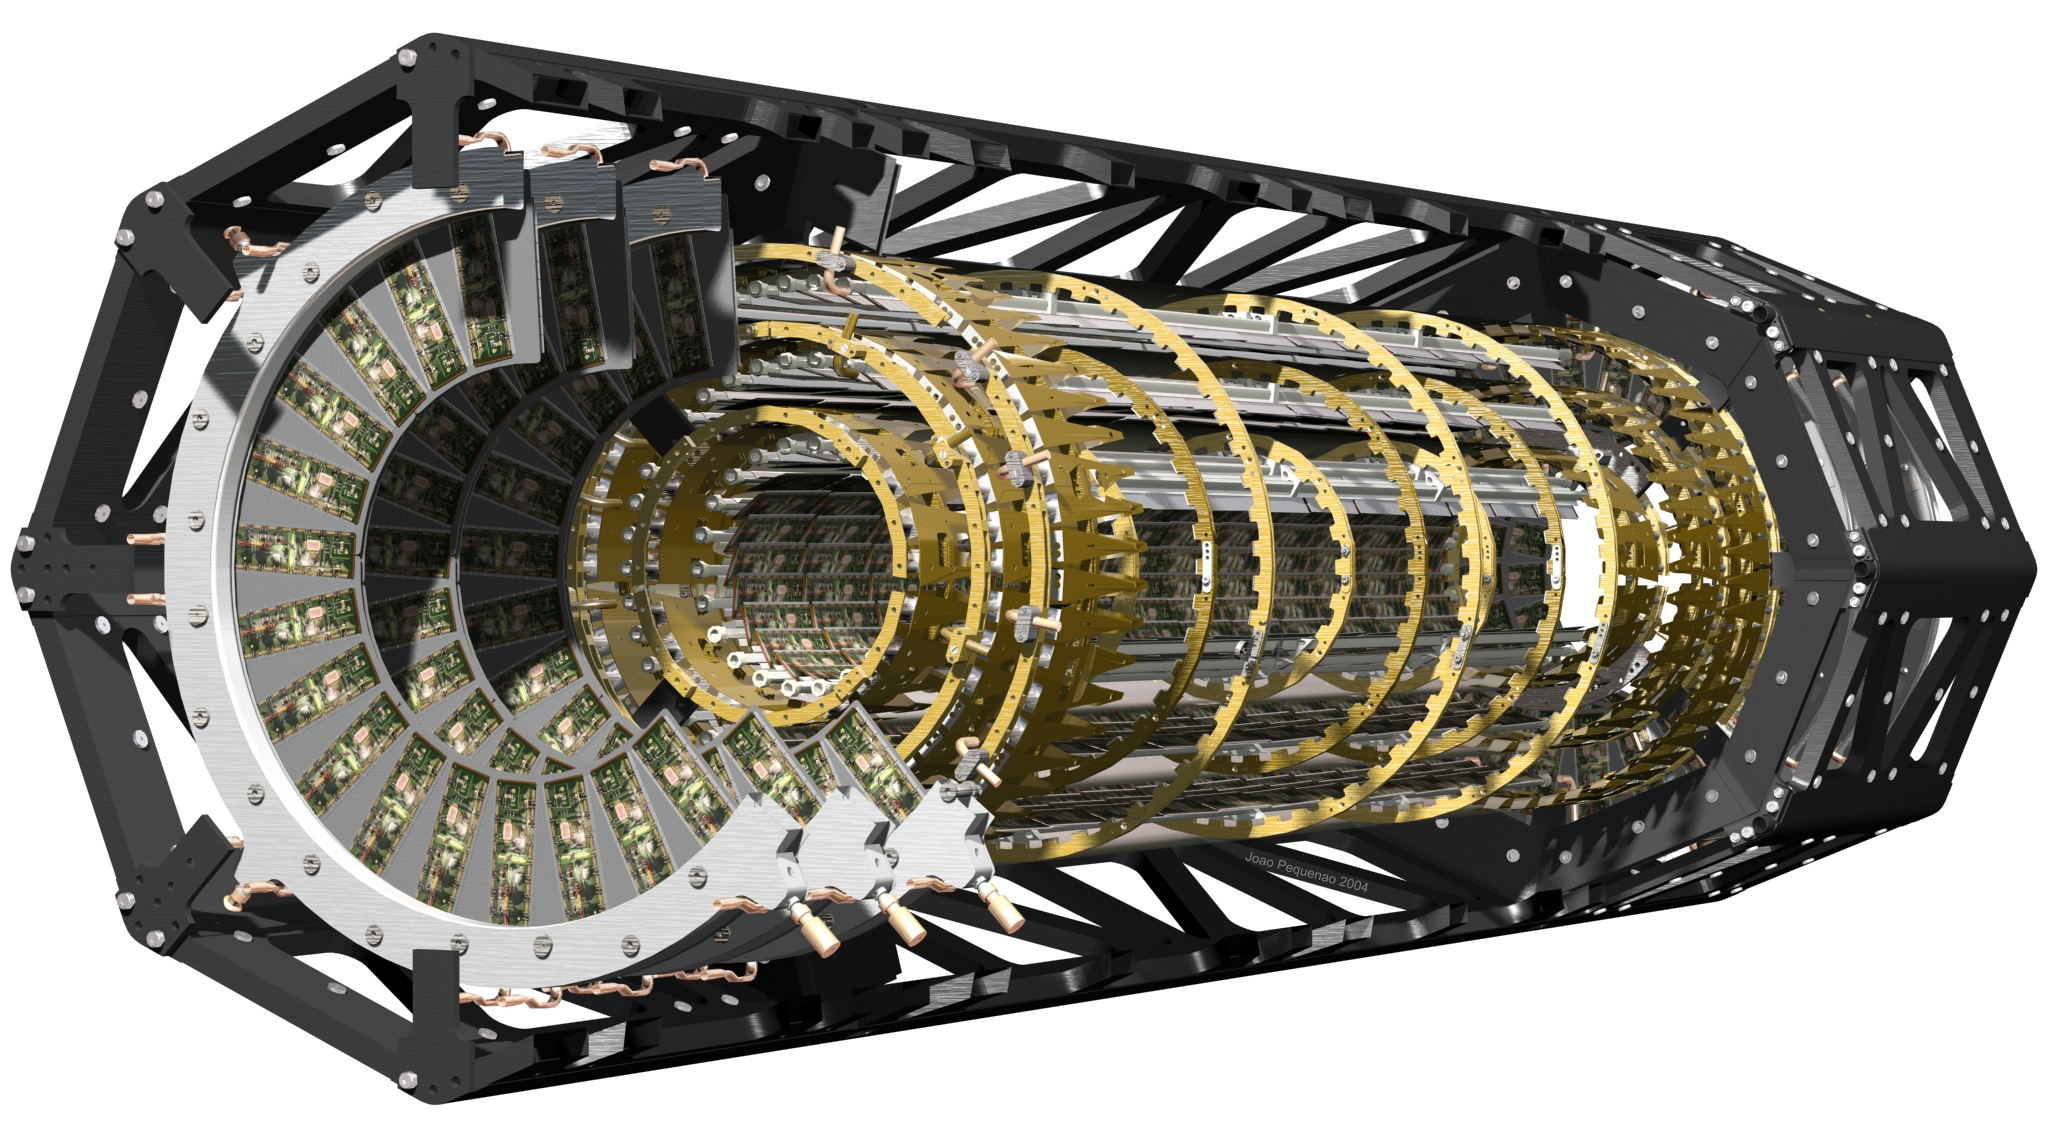
\includegraphics[width=0.7\textwidth]{pixel.jpg}
\label{fig:detector:pixel}
\caption{A computer-generated view of the ATLAS pixel detector. Copyright CERN.}
\end{figure}

%%%%%%%%%%%%%%%% 



\subsection{Silicon Strip Tracker}

The next outermost subdetector in the ID is composed of silicon microstrip layers~\cite{SCTPaper,ATLASPaper}, and is commonly referred to as the SCT.  The SCT operates under a very similar principal to the Pixel detector: doped silicon under an electric bias is the active medium, and electron/hole pairs are collected to read out hits. Unlike the Pixels, one dimension of the detector is ganged together to form the eponymous strips. Two sets of detectors must therefore placed perpendicularly to each other (or at some other angle) to provide a true two-dimensional measurement, but the number of channels to be read out has been significantly reduced~\cite{Detectors}.

The ATLAS SCT contains 4088 modules, each composed of two 64 mm silicon strip sensors with a 40-mrad angular offset~\cite{ATLASPaper}. Like the Pixels, the detector is arranged into radial layers in the barrel and disks in the endcap, of which there are 4 and 9 respectively. The strips have a resolution of $17 \times 580$ in $R-\phi$ and $z$ respectively in the barrel, and $17 \times 580$ in $R-\phi$ and $R$ in the disks. The SCT occupies the space between 275 mm and 560 mm from the beamline. The detector contains a total of 6.3 million read out channels read out by radiation hard front-end chips~\cite{SCTReadout}. The increased distance of the SCT from the beamline significantly lowers the rate of expected radiation damage, but increased bias voltages are still expected to be necessary after significant luminosity~\cite{SCTPaper,ATLASPaper}.  Figure~\ref{fig:detector:sct} shows one segment of the SCT endcap disks.


%%%%%%%%%%%%%%%%

\begin{figure}
\centering
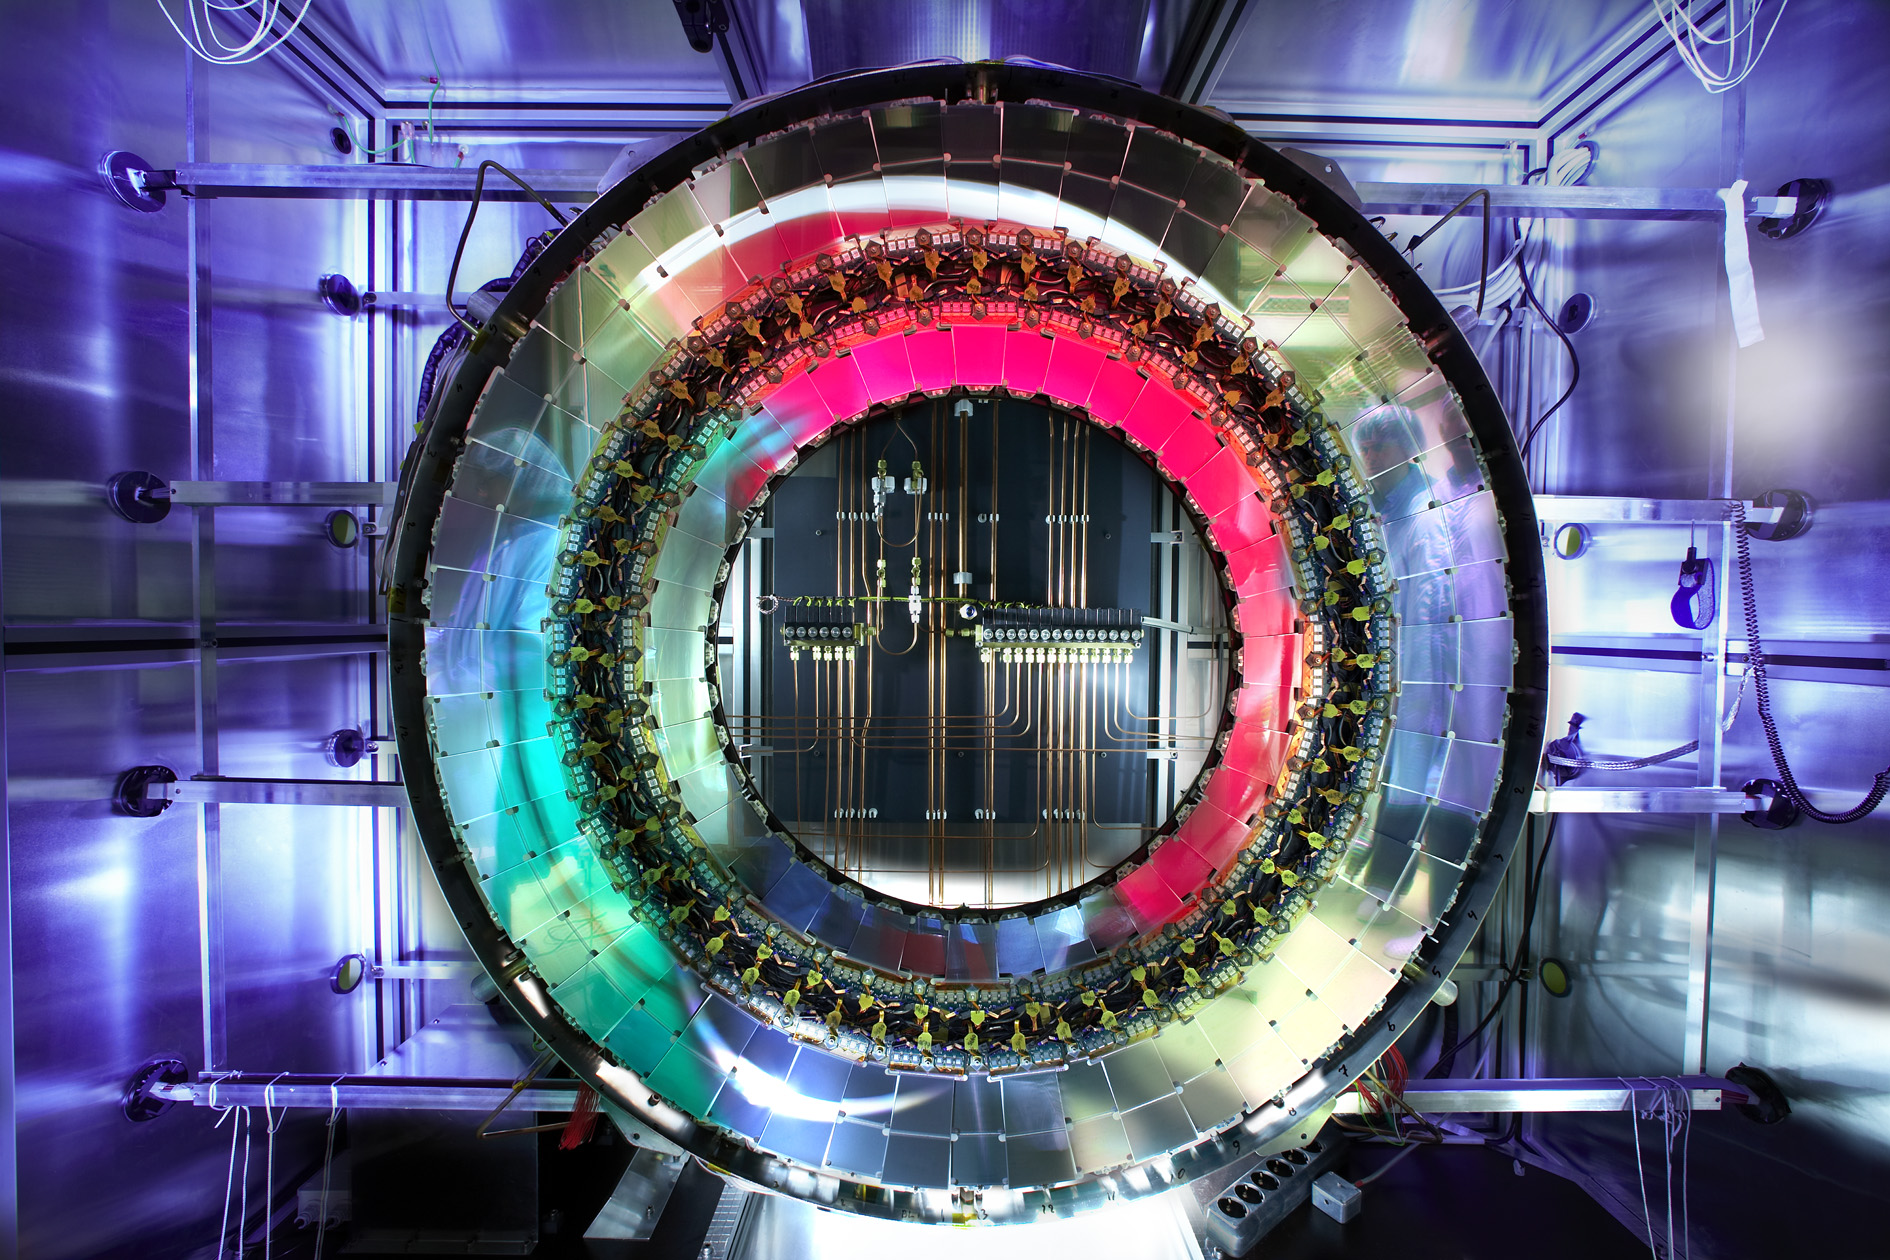
\includegraphics[width=0.7\textwidth]{sct.jpg}
\label{fig:detector:sct}
\caption{A photograph of one segment of the ATLAS SCT endcap disks. Copyright CERN.}
\end{figure}

%%%%%%%%%%%%%%%% 

\subsection{Transition Radiation Tracker}
\label{detector:ID:TRT}
The final subdetector of the ID is the transition radiation tracker~\cite{ATLASPaper}. Unlike the other subdetectors of the ID, the TRT is not made out of silicon: instead, it is composed of 2 mm (in radius) straw tubes (proportional drift tubes)~\cite{ATLASPaper}. The tubes detect particles via ionization: particles traversing the tube interact with the gas in the tube (70 $\%$ Xe, 27 \% CO$_2$, and 3 \% O$_2$) and create ion/electron pairs~\cite{Detectors,ATLASPaper}. The exterior of the tube is a cathode, and a center wire is an anode, set at a voltage difference of 1530 V. The extreme electric field in the tube accelerates the electrons rapidly through the gas, colliding with other atoms and creating more ion/electron pairs, creating an avalanche which greatly amplifies the original signal~\cite{Detectors}. The time of arrival of the signal to the anode depends on the position of the initial collision and the known drift velocity of the gas, thus allowing for an accurate radial measurement of the interaction point~\cite{TRTReadout}, but no information about the location of the interaction along the length of the tube.

The TRT covers the range $|\eta| < 2.0$ in the standard barrel and endcap arrangements~\cite{TRTPaper}. There are 52544 tubes, each 1.44 m in length, arranged in two active regions on either side of the center of the detector. The endcaps are each composed of 122880 370 mm long tubes, organized into 18 wheels. The barrel is arranged in layers of 76 straws, while the endcaps have 160 planes. There are a combined 350848 channels in the detector. Figure~\ref{fig:detector:trt} shows a photograph of the TRT barrel during testing.

The TRT, whose active elements are much larger than that of the silicon sensors in the rest of the ID, has a significantly larger hit resolution: 130 $\mu$m in $R-\phi$~\cite{ATLASPaper}. This is partly compensated by the large number of straws that charged particles cross, generating on average 30 hits~\cite{ATLASExpected}. The TRT has the added benefit of providing identification of electrons via the emission of transition X-rays~\cite{TRTPID}. X-ray photons can be emitted as a relativistic electron passes through materials with different dielectric constants; the X-rays can subsequently interact with the straw tube gas and cause an ionization with a much higher energy than for a direct hit (15 keV, compared to 2 keV)~\cite{TRTReadout}. This extra energy can be recorded and used later for identification of the electron. In the barrel, the TRT straws are embedded in a set of polypropylene-polyethylene fibers with a diameter of 19 $\mu$m; in the endcap, foil is interleaved between the straws. This type of identification is not possible with silicon detectors, providing the TRT with a unique capability. Finally, the gas tubes of the TRT present a significantly lower amount of material to particles traversing the ID compared to silicon detectors, thereby degrading less the performance of the ECal and HCal.

Given the distance of the TRT from the interaction point, and the greater resilience of gas tubes to radiation compared to silicon (there is no atomic lattice to be damaged), the TRT is not expected to be significantly damaged during the course of data-taking. However, with the presence of increasing pileup conditions in upcoming runs, the occupancy of the TRT is expected to grow significantly, presenting a significant challenge to continued operation~\cite{TRTOccupancy}.

%%%%%%%%%%%%%%%%

\begin{figure}
\centering
\includegraphics[width=0.7\textwidth]{trt.jpg}
\label{fig:detector:trt}
\caption{A photograph of the ATLAS TRT system during testing. Copyright CERN.}
\end{figure}

%%%%%%%%%%%%%%%% 

\section{Calorimeters}

The ATLAS calorimeters lie outside of the ID and the solenoid, and are responsible for a near-hermetic ($|\eta| < 4.9$) measurement of all particles except for muons and neutrinos~\cite{ATLASPaper}.  The calorimeter system is also critical in stopping particles (besides muons) from entering the muon spectrometer. The calorimeters are the primary detectors of interest in the reconstruction of hadronic events, as they are the only detectors capable of measuring neutral particles which the tracker can miss. The operation of these detectors is thus critical for both searches for new physics in hadronic channels, and for measurements of hadronic phenomena in the Standard Model.

The combined calorimeter system is pictured in Figure~\ref{fig:detector:calo}. There are several subsystems: the LAr electromagnetic barrel, the tile barrel, tile extended barrel, the LAr electromagnetic endcap (EMEC), the LAr hadronic endcap (HEC), and the LAr forward calorimeter (FCal)~\cite{ATLASPaper}. The central LAr barrel also has a presampler layer, which estimates the energy lost before the particles reach the ECal.

All the detectors are non-compensating, sampling designs. Sampling detectors are designed in alternating layers of passive absorber and active readout. The passive layers are composed of some dense material (steel, lead, etc.) which, because of the high density of atoms, causes many interactions with the incoming particles, creating cascades of daughter particles. The active layers measure the energy of the showers-- via mechanisms such as scintillation or ionization-- and the process repeats several times, gradually reducing the energy of the shower with each layer and thereby stopping the particles. The non-compensating nature of the calorimeter means that energy is lost in each of these passive layers: the full energy read out by the active layers will not be that of the incoming particles. Calibrations, described in later sections \editnote{Fix that!} can correct for the central value of this unmeasured energy, but fluctuations in the shower development inevitably mean that there is a price in terms of energy resolution~\cite{Wigmans}. The details of homogenous vs. sampling, and compensating vs. non-compensating designs depend greatly on the conditions of the collider, and the designs selected by ATLAS were chosen based on the compromises between expected performance gains and cost. 



%%%%%%%%%%%%%%%%

\begin{figure}
\centering
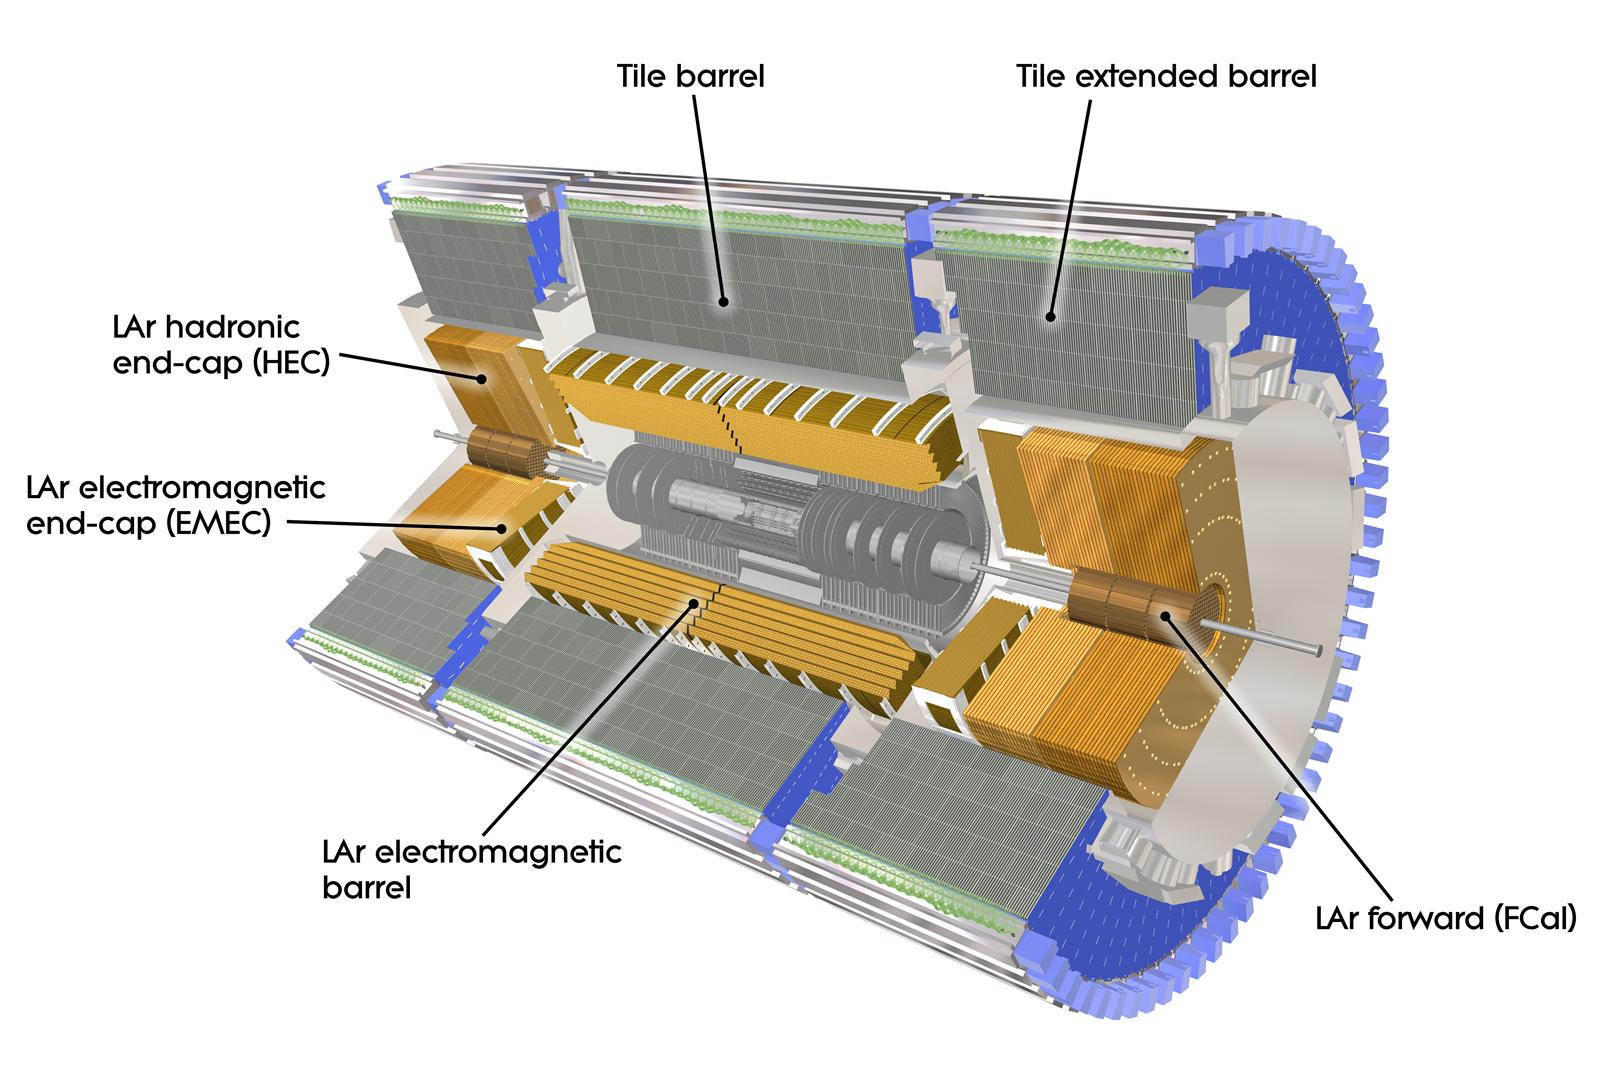
\includegraphics[width=0.7\textwidth]{calorimeters.jpg}
\label{fig:detector:calo}
\caption{A computer generated image of the ATLAS calorimeter system, showing the locations of each different subdetector. Copyright CERN.}
\end{figure}

%%%%%%%%%%%%%%%% 


\subsection{Electromagnetic Calorimeter}

Like many of the other detectors, the ECal is composed of two main sections; the barrel and the endcaps~\cite{ATLASPaper}. The barrel covers the range $|\eta| < 1.475$, and occupy the space between 2.8 m and 4 m from the beamline. The detector is a total of 6.4 m long. Both use lead as the passive layer and liquid argon as the active material. A presampler covers the entire $\eta$ range of the barrel.

The endcaps consist of two wheels, on either side of the detector, and cover the range $1.375 < |\eta| < 3.2$ and occupy the region between 330 mm and 2098 mm from the beamline\footnote{Note that this is the first detector component listed that sits outside of the tracker volume in $z$, and so is not limited by the tracker's radial size.} A presampler also covers the region in front of the endcap.

The LAr calorimeters all operate via the measurement of ionization~\cite{Detectors,Wigmans}. As particles-- particularly photons and electrons which interact predominantly electromagnetically-- interact with the liquid argon, they knock free electrons and create ions. The high voltage applied across opposite ends of the detector drifts the free electrons to one side, where they can be measured. The passive lead layers promote electromagnetic showering which can be read out by the active material, while also providing a large number of radiation lengths to absorb the energy of these particles.

The barrel system is composed of 2048 so-called ``accordion-shaped'' absorbers, instrumented with interleaved readout electrodes~\cite{ATLASPaper}. The characteristic accordion shape, displayed in Figure~\ref{fig:detector:lar-accordion}, is designed to reduce the drift time after a particle interacts but before the ionization energy has been collected. Depending on the $\eta$, there are between 3 and 4 separately read-out layers, in addition to the presampler, in each module. The size of the detector cells which are read out depends on the layer, as shown in Figure~\ref{fig:detector:lar-module}. 

%%%%%%%%%%%%%%%%

\begin{figure}
\centering
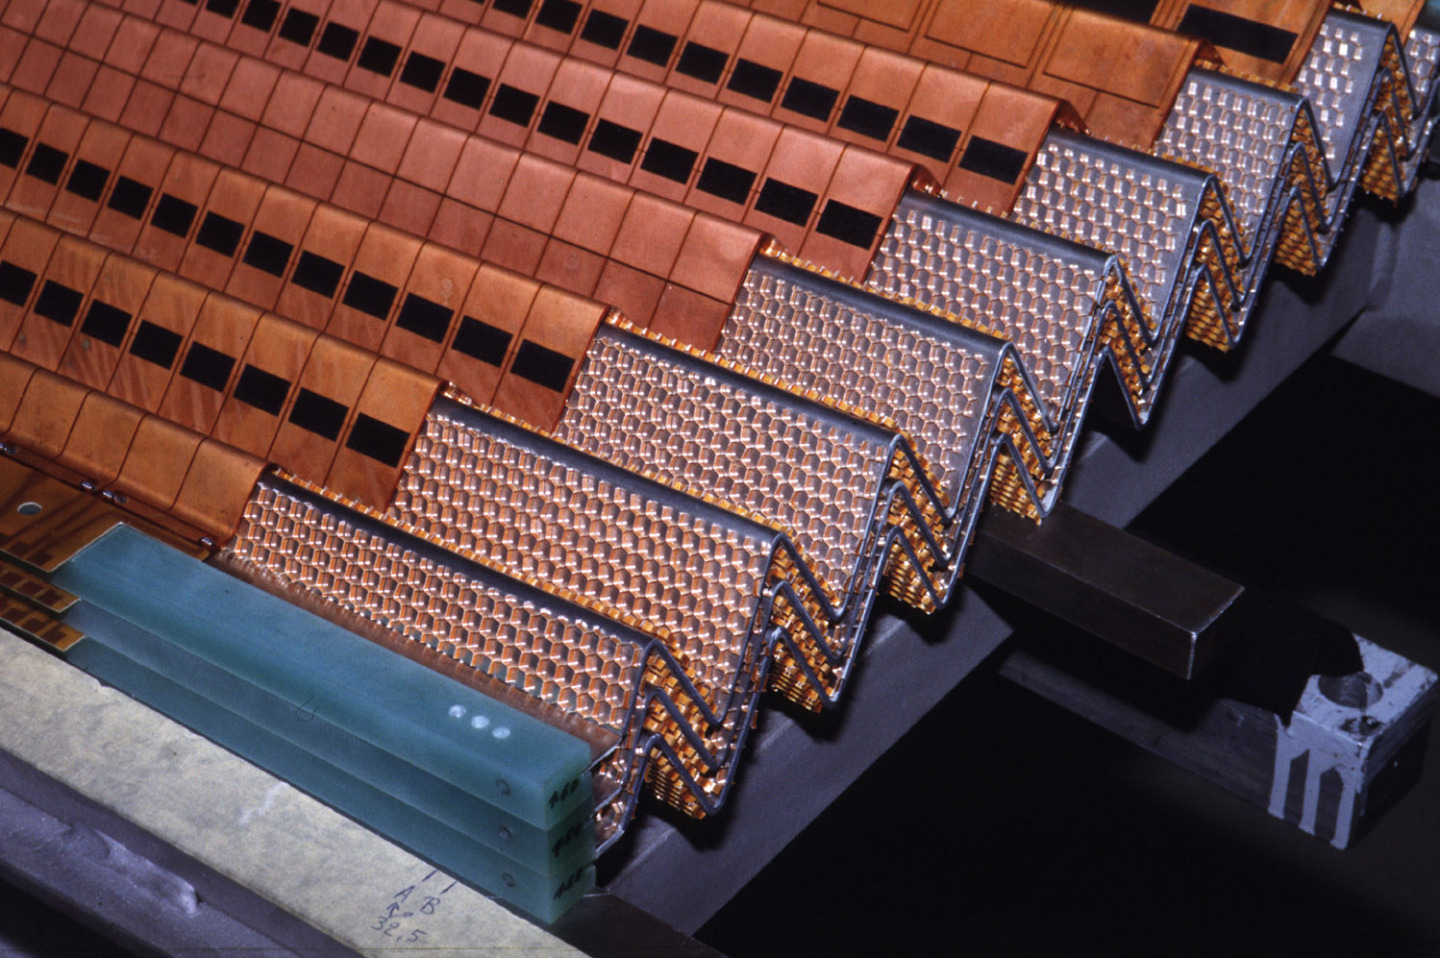
\includegraphics[width=0.7\textwidth]{lar-accordion.jpg}
\label{fig:detector:lar-accordion}
\caption{A photograph of the accordion structure used in the LAr barrel. Copyright CERN.}
\end{figure}

%%%%%%%%%%%%%%%% 

%%%%%%%%%%%%%%%%

\begin{figure}
\centering
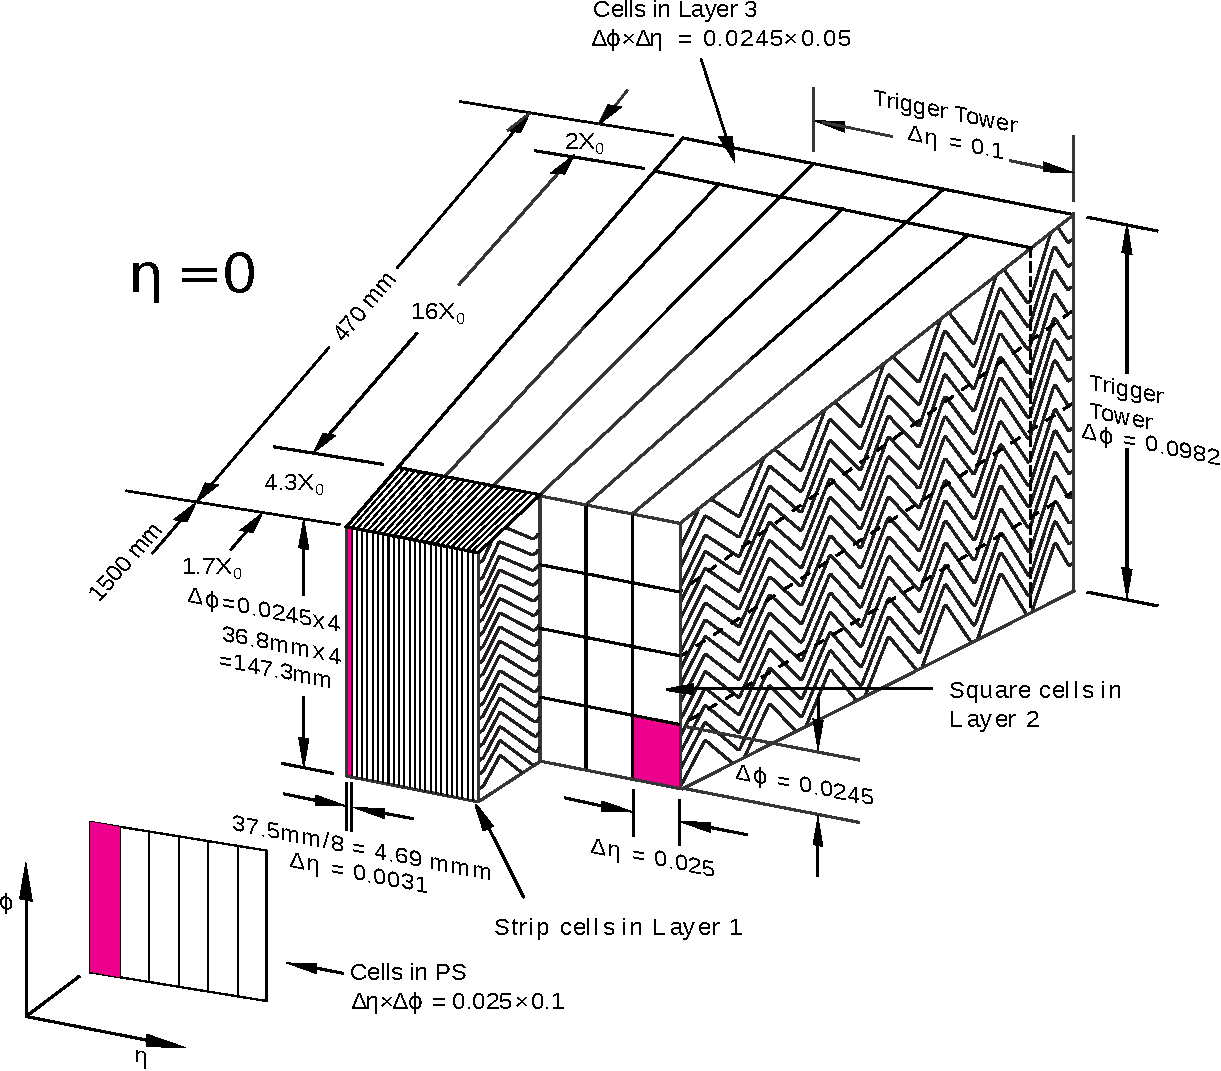
\includegraphics[width=0.7\textwidth]{lar-module.pdf}
\label{fig:detector:lar-module}
\caption{A drawing of a LAr module near $\eta = 0$. The relative size of each layer in the module, in both length and radiation lengths, is shown.}
\end{figure}

%%%%%%%%%%%%%%%% 



The endcap follows a similar design, separated into two sub-wheels per wheel~\cite{ATLASPaper}. The outer wheel (at lower values of $|\eta|$) is composed of 768 absorbers with three layers, and the inner wheel (at higher values of $|\eta|$) is composed of 256 absorbers with only two layers. The granularity of the outer wheel is similar to that of the barrel calorimeter, but the inner wheel has a coarser granularity.\footnote{Note though that while the granularity is worse in $\eta$, the coordinate is asymptotic as $\theta$ increase and the physical granularity of the inner wheel is not worse.} Figure~\ref{fig:detector:lar-endcap} shows a photograph of one of the LAr endcaps after its installation in the detector.


%%%%%%%%%%%%%%%%

\begin{figure}
\centering
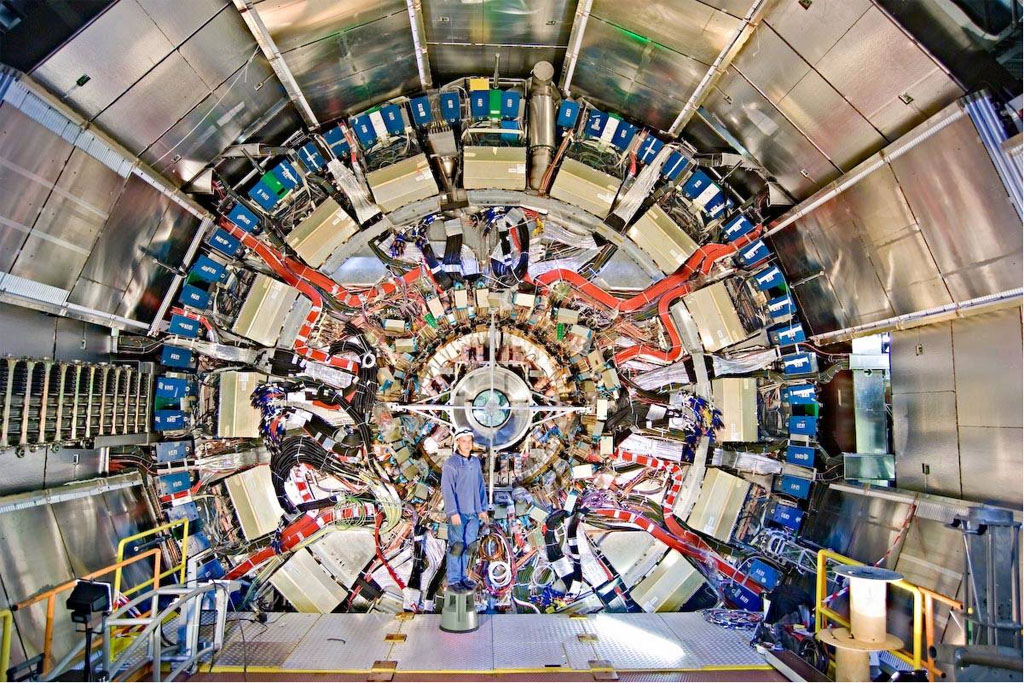
\includegraphics[width=0.7\textwidth]{lar-endcap.jpg}
\label{fig:detector:lar-endcap}
\caption{A photograph of the LAr endcap after installation in the cryostat system. Copyright CERN.}
\end{figure}

%%%%%%%%%%%%%%%% 

Both detectors operate at voltages of approximately 2 kV~\cite{ATLASPaper}. The barrel occupies a cryostat shared with the solenoid, and is cooled by a nitrogen refrigerator system which operates at 80 K. The endcaps each share a cryostat with the HEC and FCal, and are cooled by a similar nitrogen system.

A benefit of using liquid argon as a readout material is that it is readily purified and relatively inexpensive, and so can easily be used in large volumes. A drawback is the long collection time of the ionization energy, typically of order 450 ns, which is complicated by the LHC's design of collisions every 25 ns~\cite{ATLASPaper,LARPaper}. This means that after a particle has left an energy deposit in the calorimeter in one bunch crossing, it remains for up to 16 subsequent bunch crossings. This effect is referred to as ``out-of-time'' pileup. One solution to this issue is to exploit the very consistent and well understood characteristics of the ionization pulse, and to shape it (via the readout electronics) to compensate for out-of-time pileup. This is demonstrated in Figure~\ref{fig:detector:lar-pulse}: a bipolar $CR -(RC)^2$ analogue filter generates a fast time constant for the rise and fall (13 ns), resulting in a negative energy portion of the pulse~\cite{LARPaper}. This negative energy portion has the same integrated area as the positive portion: on average, the negative portion should cancel the in-time component of pileup from subsequent collisions~\cite{Loch}. The very predictable pulse shape also simplifies the readout: only the first five points need to be read out to predict the full shape, as shown in Figure~\ref{fig:detector:lar-pulse-2}. Of course, the ECal is also susceptible to in-time pileup, as the detector does not have enough position resolution to identify whether an energy deposit occured from the primary hard-scatter or additional primary vertices.

%%%%%%%%%%%%%%%%

\begin{figure}
\centering
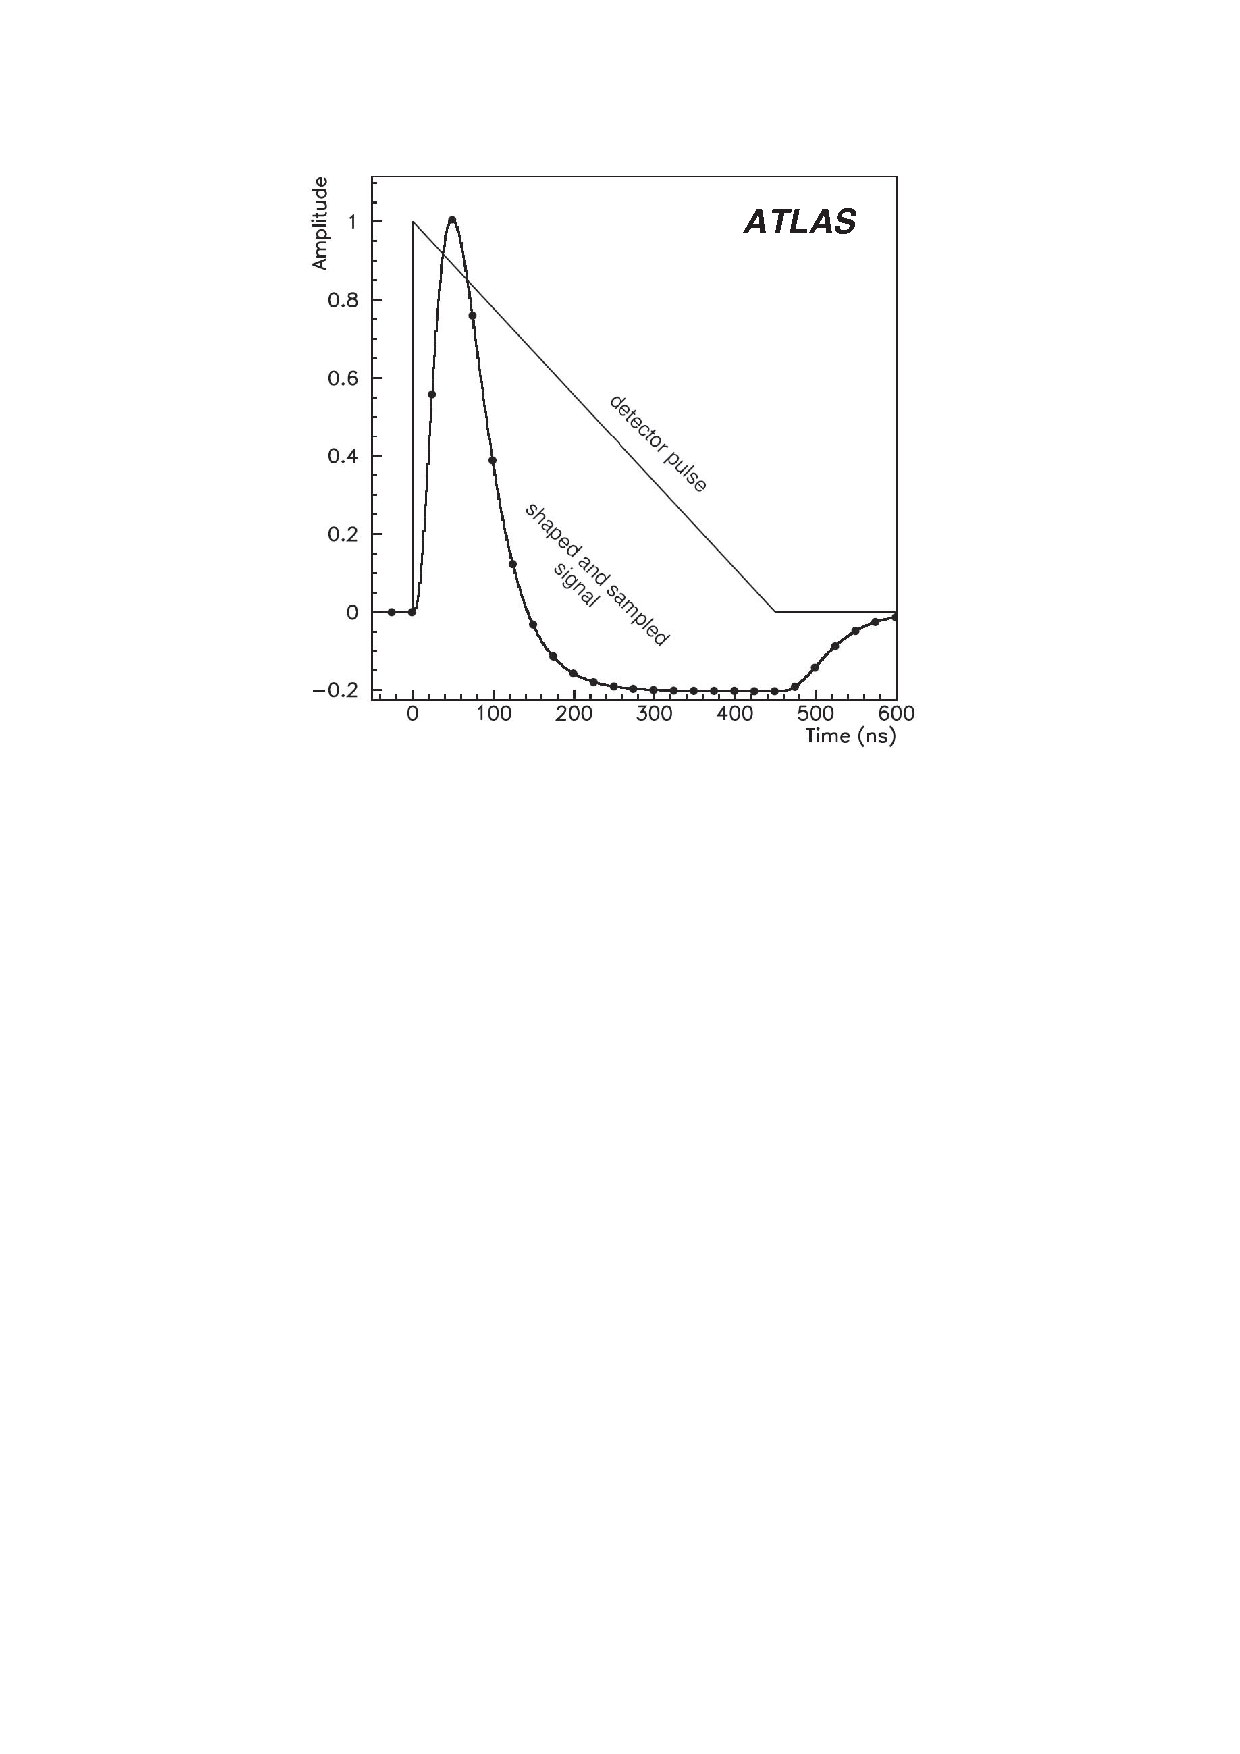
\includegraphics[width=0.7\textwidth]{lar-pulse.pdf}
\label{fig:detector:lar-pulse}
\caption{A plot of the LAr ionization pulse and the shaped output from the frontend electronics, including the negative energy region.}
\end{figure}

%%%%%%%%%%%%%%%% 

%%%%%%%%%%%%%%%%

\begin{figure}
\centering
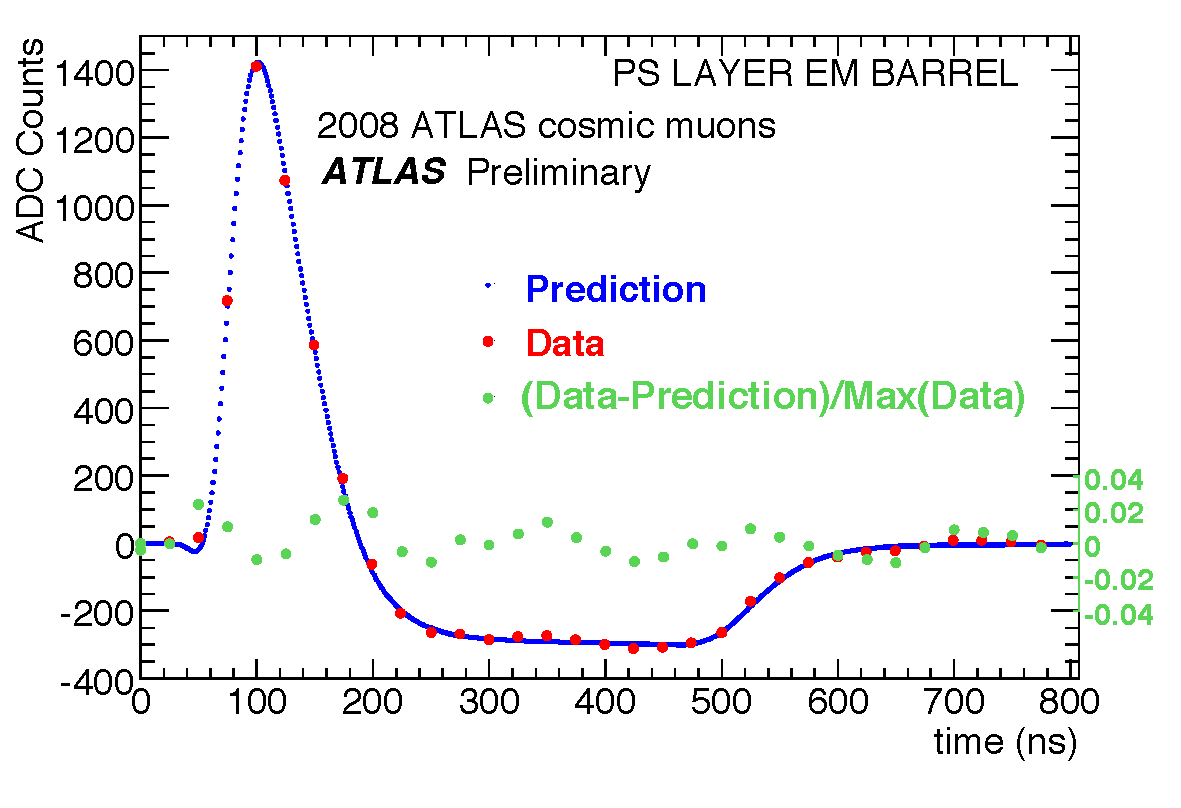
\includegraphics[width=0.7\textwidth]{lar-pulse-2.pdf}
\label{fig:detector:lar-pulse-2}
\caption{A plot the measured and predicted LAr energy distributions during a 2008 cosmic ray run.}
\end{figure}

%%%%%%%%%%%%%%%% 

As the liquid argon in the detector can be continuously filtered, there is no danger of damage due to radiation (in contrast to the CMS homogenous crystal calorimeter, which `darkens' over time). Future upgrades include the goal of reading out at a higher rate and with potentially greater granularity, especially at the trigger level.



\subsection{Hadronic Calorimeter}

The Hadronic Calorimeter is composed of four subsystems: the tile barrel, the tile extended barrel, the LAr hadronic endcap, and the LAr forward calorimeter. 

The tile systems extend to $|\eta| < 1.7$ and sit behind the LAr electromagnetic calorimeter~\cite{ATLASPaper,Tile}. The barrel detector is 5.8 m long, and each of the extended barrels are 2.6m long. The detectors each have an inner radius of 2.28 m and an outer radius of 4.25 m. The combined detector is shown, after installation the ATLAS cavern, in Figure~\ref{fig:detector:barrel-tile}. The detectors are composed of 64 wedge-shaped modules with size $\Delta\phi \approx 0.1$, an example of which is pictured in Figure~\ref{fig:detector:tile-wedge}. The detector is composed of alternating layers of steel plates and plastic scintillating tiles: by volume the steel-to-tile ratio is approximately 4.7:1 and is almost exactly periodic. The detector operates via similar principles to that of the ECal: particles (which at this depth in the detector are mostly hadrons) interact with the steel and produce showers of lower energy particles. These particles proceed through the scintillator: as they pass through a material where the speed of light is lower than their current speed, they emit scintillation light, which can be collected by readout fibers and read out by photomultiplier tubes~\cite{Wigmans,Detectors,Tile}. An example of one of the scintillating tiles is pictured in Figure~\ref{fig:detector:actualtile}. Like the ECal, the tile calorimeter contains three independently readout layers, which provies information about the longitudinal development of the particle shower. The front two layers are readout in $\Delta \eta \times \Delta\phi$ cells of approximately  $0.1 \times 0.1$ for the front two layers, and and $0.2 \times 0.1$ for the third layer.

Unlike the LAr systems, the tile calorimeters have a fairly quick readout, and are not affected by out-of-time pileup. Because the tile system sits behind so many other detectors, and pileup particles are generally rather soft to begin with and are usually stopped by the upstream detectors, even in-time pileup is expected to have a much lower effect than on the ECal.

The hadronic endcap system is similar to the ECal, but is composed of alternating layers of copper and liquid-argon with a flat design (in contrast to the ECal's accordion shape)~\cite{ATLASPaper}. The detectors occupy the range $1.5 < |\eta| < 3.2$, and they share the end-cap cryostats with the EMEC and FCal.  Each HEC endcap is composed of two wheels, each of of which has two longitudinal layers. Each of the four wheels is cylindrical, with an outer radius of 2.03 m, and each of the wheels is composed of 32 wedge-shaped modules. The read-out cells have size $\Delta \eta \times \Delta\phi = 0.1 \times 0.1$ for $|\eta| < 2.5$, and $0.2 \times 0.2$ for larger values. The LAr ionization readout uses high-voltage set to 1800 V.

The ATLAS forward calorimeters are the final devices in the end-cap cryostats, and sit in the highest pseudorapidity, covering $3.1 < |\eta| < 4.9$~\cite{ATLASPaper}. The FCal is composed of three 45 cm modules: FCal1 is an electromagnetic module, and FCal2 and FCal3 are hadronic modules. Copper is used as the absorber in FCal1, and tungsten is used in FCal2/3. All three use liquid argon as the active medium.

The HCal systems are all expected to perform very well in future LHC runs, even with increased pileup conditions. Upgrades to some of the readout systems to enable more rapid and more regular collection of data are the main goals in preparation for higher luminosity operations.

\editnote{This feels sparse somehow. What's missing?}

%%%%%%%%%%%%%%%%

\begin{figure}
\centering
\includegraphics[width=0.7\textwidth]{tile.jpg}
\label{fig:detector:barrel-tile}
\caption{A photograph of the installation of the barrel tile calorimeter. Copyright CERN.}
\end{figure}

%%%%%%%%%%%%%%%% 

%%%%%%%%%%%%%%%%

\begin{figure}
\centering
\includegraphics[width=0.7\textwidth]{tile-wedge.pdf}
\label{fig:detector:tile-wedge}
\caption{A drawing of one wedge of the tile detector.}
\end{figure}

%%%%%%%%%%%%%%%% 

%%%%%%%%%%%%%%%%

\begin{figure}
\centering
\includegraphics[width=0.7\textwidth]{tile-actualtile.jpg}
\label{fig:detector:actualtile}
\caption{A photograph of one of the scintillating tiles which give the tile calorimeter its name. Copyright CERN.}
\end{figure}

%%%%%%%%%%%%%%%% 




\section{Muon Spectrometer}

The Muon Spectrometer (MS) is the outermost detector in ATLAS~\cite{ATLASPaper}. It is designed to accurately reconstruct charged particles which exit the calorimeters out to $|\eta| < 2.7$, and can trigger on these particles to $|\eta| < 2.4$. A break for calorimeter and cryostat servies at $\eta \approx 0$ reduces the efficiency for vertical muon reconstruction.  Unlike the other detectors, which are designed to measure many different types of particles, in practice the goal of the muon spectrometer, as its name suggests, is to measure only muons, as those are typically the only particles which interact so weakly that they can pass through the calorimeter systems. The MS is capable of reconstructing tracks independently, but muon reconstruction is typically performed in a ``combined'' mode of operation, where independently reconstructed ID and MS tracks are matched to create muon candidates with improved momentum measurements. Because the toroid magnets bend particles in a direction perpendicular to that of the solenoid surrounding the ID, the measurements of the ID and MS are largely independent and increase the precision of the measurement. This is contrast to the CMS muon system, which only provides a ``tag'' which labels the muon and the ID performs the full momentum measurement.

The different subsystems of the MS are shown in Figures~\ref{fig:detector:ms} and \ref{fig:detector:ms-eta} as a computer-generated image of the whole detector and as a schematic drawing in the $z-\eta$ plane respectively. Note that Figure~\ref{fig:detector:ms-eta} shows the MS in the bending plane of the toroids: curved trajectories in this direction are measured to extract the momenta of particles. 


%%%%%%%%%%%%%%%%

\begin{figure}
\centering
\includegraphics[width=0.7\textwidth]{muons.jpg}
\label{fig:detector:ms}
\caption{A computer generated image showing the locations of each of the muon spectrometer subsystems. Copyright CERN.}
\end{figure}

%%%%%%%%%%%%%%%% 

%%%%%%%%%%%%%%%%

\begin{figure}
\centering
\includegraphics[width=0.7\textwidth]{muon-eta.pdf}
\label{fig:detector:ms-eta}
\caption{A drawing in the $z/\eta$ plane showing the location of the various detector subsystems in the MS. This is the bending plane of the toroids, so infinite momentum particles would have straight trajectories in this view and others would be curved.}
\end{figure}

%%%%%%%%%%%%%%%% 

The largest subsystem of the MS are the Monitored Drift Tube chambers (MDT's), which provide precision measurements of charge particle hits~\cite{ATLASPaper}. There are 1088 MDT chambers in the detector, covering a total area of 5500 m$^2$. Chambers are composed of several layers of the eponymous tubes, and the precise number of tubes in each chamber varies between 48 and 432. The chambers are arranged into three layers in the barrel and three wheels in the endcap (though at high $\eta$ values only two layers of MDT are used due to the higher particle flux). The tubes themselves are proportional drift chambers with an Ar/CO$_2$ gas mixture at $93\%/7\%$ respectively ~\cite{ATLASPaper,Detectors}. Ionization electrons are collected by a central tungsten-rhenium wire, held at a potential of 3080 V. Similar to the TRT described in Section~\ref{detector:ID:TRT}, the drift tubes provide only one coordinate measurement, this time in the $z$ direction to take advantage of the toroid bending axis. The non-measured coordinate of a hit is provided by the triggering detectors, described below. The MDTs provide a typical resolution of 35 $\mu$m in the $z$ direction, and muons typically cross 20 tubes as they are measured. The maximum readout time of an MDT is approximately 700 ns-- to prevent overlapping measurements from different collisions, the readout system implements a dead-time after the first detection of charge.
 
Cathode-Strip Chambers (CSC) sit in the forward region of $2.0 < |\eta| < 2.7$, and are used in track reconstruction in the $2.0 < |\eta| < 2.7$ region where the MDTs have only two layers, both of which appear after the CSC~\cite{ATLASPaper}. The CSC chambers are arranged in four consecutive planes in each wheel, for a total of 32 chambers; each plane is composed of perpendicular strips which allow for the measurement of both coordinates of a hit. The CSCs provide fewer hits than an equivalent layer of MDTs, but have fewer readout inefficiencies due to their faster response time. The CSC's are multiwire proportional chambers whose wires are oriented in the radial direction. The anodes of the detector are the wires, and the sides (in the $R$ and $\phi$ directions) are instrumented cathodes which readout the ionization of the Ar/CO$_2$ gas mixture (operated at $80\%/20\%$)~\cite{Detectors,ATLASPaper}. The detectors are operated at 1900 V, and have typical drift times of much less than 40 ns. The fine segmentation of the cathodes in both coordinates allows for very currate position resolution, allowing for typical resolutions of 40 $\mu$m in $R$ and 5 mm in $\phi$.

In addition to the precision measurement systems, the MS contains two systems used primarily for triggering. The Resistive Plate Chambers (RPC) are used in the barrel region of $|\eta| < 1.05$, and Thin Gap Chambers (TGC) are used in the endcap ($1.05 < |\eta| < 2.4$). The detectors are meant to measure the non-bending coordinate of the track to complement the MDT measurements, and to provide a complete, fast, and coarse tracking for use in the trigger. 

RPCs are parallel plate ionization detectors, and measure hits through the ionization of gas~\cite{Detectors,ATLASPaper}. The plates are kept 2 mm from each other, with an electric field of 4.9k kV/mm. The plates are segmented for the purposes of readout, allowing for local determination of hit coordinates. RPCs are typically paired with MDT stations, allowing the non-bending coordinate measured by the RPC to be used by the MDT hit. The RPCs have a typical hit resolution of 10 mm in $z$ and $\phi$, and muons typically cross 6 detectors. 

TGCs are multi-wire proportional chambers similar in design to the CSCs. \editnote{Check this statement?} The bending coordinate is measured by collection of charge on the TGC wire, while the other is measured by radial strips in the cathode. The detector is arranged into circular disks mounted in two concentric rings. The TGCs have a typical hit resolution of $2-6$ mm in $R$ and 3-7 mm in $\phi$, and muons typically cross 9 detectors.

While the vast majority of the use of the MS comes from its measurement of muons, it provides some additional use in the study of hadronic physics (besides measuring muons from semi-leptonic decays) by enabling the measurement of punch-through~\cite{JES2010}. Some jets-- either because of parton shower fluctuations or because they are extremely high energy-- are not stopped entirely by the calorimeter system. Because all the calorimeters are sampling, this means that some portion of the energy of the jet is also not measured. However, these particles can still proceed through the MS and leave hits in the detectors, as seen in Figure~\ref{fig:detector:punchthrough}. These hits can be used to create on-average corrections for punchthrough, and can thereby improve the energy measurement of jets in an unusual way.

While the detectors of the MS are not expected to need replacement due to radiation (the choice of detector gas was often motivated to guarantee this, in fact), issues of readout optimization and occupancy do arise at higher luminosity.In particular, the CSC readout has been completely redesigned for Run II in order to provide measurements at a much higher rate in order to assist in muon triggering. \editnote{Is this correct?}

\editnote{Is this good? A bit unbalanced, but probably fine considering I don't really care about muons.}

%%%%%%%%%%%%%%%%

\begin{figure}
\centering
\includegraphics[width=0.7\textwidth]{punchthrough.pdf}
\label{fig:detector:punchthrough}
\caption{A portion of an event display showing a high $p_T$ jet (176 GeV) with 128 measured hits in the muon spectrometer.}
\end{figure}

%%%%%%%%%%%%%%%% 

\section{Forward Detectors}

In addition to the main detectors described in the previous sections, several forward detectors (some even located outside of the main volume) provide additional information used in luminosity measurements and some triggering applications~\cite{ATLASPaper}. The luminosity measurements are particularly critical for searches for new physics, and for understanding of the accelerator conditions. The radiation-hard diamond Beam Conditions Monitor (BCM), for example, is place at $\pm$ 1.84 m in $z$ and use a fast response time (2 ns) to distinguish between collision events and beam anomalies. The Minimum-Bias Trigger Scintillators (MBTS), placed at $\pm 3.56$m, are fast-responding plastic scintillators used to trigger on collisions that do not leave large energy signatures in the central detectors. The LUminosity measurement using a Cerenkov Integrating Detector (LUCID) follows the terrible naming conventions developed by ASCOT and ATLAS. It measures the luminosity by measuring the $pp$ elastic cross-section with two very far forward detectors, placed at $\pm$ 17 m and 100 mm in $r$. The detectors consist of aluminum tubes filled with scintillating gas readout by PMTs, enabling measurements of the luminosity to 25$\%$ precision.

\section{Triggering}

With collisions occuring every 25 ns at design luminosity, and even every 50 ns in 2012 operations, ATLAS has no chance of recording every collision. Instead, a triggering system is used to quickly identify interesting events and to mark them for later analysis\cite{ATLASPaper,Trigger2010}. This system is divided into three stages: Level 1 (L1), Level 2 (L2), and the Event Filter (EF). Each stage is designed to make a decision using some limited amount of information from the detector at a maximum rate before handing off to the next stage, which can use more information to make a better informed decision. In this manner, the initial collision rate of 40 MHz (20 MHz in 2012) is reduced to 75 kHz after the L1, 3.5 kHz at L2, and 200 Hz at EF. The listed rates were design goals for the initial running of ATLAS: in practice, as much as 400-600 Hz were accepted at EF during Run 1.

\subsection{Level 1}

The L1 trigger is unique amongst the trigger subsystems in that it is implemented entirely in custom hardware, configurable with programmable firmware~\cite{ATLASPaper,Trigger2010}. The L1 accepts information from the calorimeter and muon spectrometer systems only, as the ID information takes significantly longer to readout and is not available at the rate requried for L1 decisions.  The L1 muon triggers typically require 3 hits in coincidence in either the RPC or TGC detectors, with various $p_T$ threshholds. The calorimeter trigger system is significantly more complicated. As the high level of granularity of the detector would present rate challenges for the trigger, the calorimeter is readout in $0.1\times0.1$ towers in $\eta \times \phi$ (with worse granularity at high $\eta$), and typically ignore longitudinal segmentation. These trigger towers are used as the basis for triggers for electrons, photons, taus, jets, total transverse energy $\sum E_T$, and missing energy $\MET$. The various signatures combine the towers in different ways to create the relevant physics objects: jets, for example, are searched for with a sliding window algorithm which looks at $8\times 8$ tower regions and identifies areas with significant $E_T$. Photons and electrons typically use smaller regions, and require isolation of the signal to reduce contamination from jet backgrounds.

Information from the L1 decisions are passed to the Central Trigger Processor (CTP), and data from the detector is offloaded to on-detector buffers in case an accept signal is sent~\cite{ATLASPaper}. The CTP can store up to 256 signatures, which are various combinations of muon and calorimeter information. Once the CTP sends a decision, detector buffers are transfered to the Read-Out System (ROS) via the Read-Out Links (ROLs), each of which has a Read-Out Buffer (ROB). The areas of the detector which caused the L1 trigger to fire are passed to the L2 trigger as a Region Of Interest (ROI).

\subsection{Level 2}

The L2 and EF are collectively referred to as the High Level Trigger (HLT), as they are both written in software and run on commodity computers~\cite{ATLASPaper}. Significantly more information is available at L2 as the rate has already been reduced signficantly. L2 triggers usually operate via requesting ROIs from the L1 trigger, which indicate which regions of the detector should be further inspected. The data from these regions is read into L2, and used to construct jets, tracks, photons, and so on, which can be used to make trigger decisions. As L2 has significantly more information available than L1, the algorithms used to reconstruct these objects are much closer to the offline reconstruction.

\subsection{Event Filter}

If the L2 accepts an event, the full event is read out into the Sub-Farm Inputs (SFI) and is reconstructed with no ROI restrictions~\cite{ATLASPaper}. The Event Filter then applies algorithms designed to be very close to the offline reconstruction (for example, performing topoclustering on the calorimeter cells to create inputs for jet clustering). The EF decision is performed for many events in parallel by a large network of computers-- typically each event takes 4 s to process, but the large size of the network still allows for many events to be processed in parallel. This final refinement of the detector information allows for a further significant reduction in the rate. Each readout event is approximately 1.6 MB, and is sent by the Sub-Farm Outputs (SFO) to the CERN Tier 0 datacenter for permanent storage.


\section{Data Quality}
\label{atlas:data-quality}

The Run 1 detector conditoins enabled a very high efficiency of data collection by ATLAS. Figure~\ref{fig:detector:lumi} shows the delivered LHC luminosity in the 2011-2012 period in green, and the recorded ATLAS data in yellow, with the final usable data in blue. The overall efficiency is close to 90$\%$, indicating high uptime of all subsystems.

%%%%%%%%%%%%%%%%

\begin{figure}
\centering
\includegraphics[width=0.7\textwidth]{atlas-lumi.pdf}
\label{fig:detector:lumi}
\caption{ATLAS recorded luminosity as a function of date in 2011 and 2012. The yellow show all data delivered by the LHC, green was recorded by ATLAS, and blue was high-quality data.}
\end{figure}

%%%%%%%%%%%%%%%% 

The detector uptime, and combined recording efficiency, is displayed in Figure~\ref{fig:detector:uptime}. All detector subsystems reported a very high uptime, with many detectors recovering data previously marked as `bad' by correcting flagged data in offline reconstruction. The remaining large portion of the inefficiency comes from the so-called ``warm start'' period, where the ATLAS pixel detector (and in early parts of the run also the SCT) ramps up its HV power supplies and preamplifiers only after the LHC has declared stable beams.

The LAr and Tile detectors critical to the hadronic analyses in this thesis both suffered several types of errors during operations. Most LAr errors were due to high-voltage power supply trips which disabled modules while the power supplies automatically recovered; most tile issues were related to problems with the low-voltage power supplies. Both of these errors were flagged during data taking so that affected events could be properly vetoed (in the case of the LAr issues) or corrected (in the case of the Tile).

%%%%%%%%%%%%%%%%

\begin{figure}
\centering
\includegraphics[width=0.7\textwidth]{DQ-eff-table2012pp-AprilDecember2012}
\label{fig:detector:uptime}
\caption{ATLAS subdetector uptime during 2012 data taking.}
\end{figure}

%%%%%%%%%%%%%%%% 



\chapter{Jet Reconstruction with ATLAS}
%!TEX root = ../swiatlow_thesis.tex
\label{chapter:jet-reconstruction}


Jet reconstruction in ATLAS makes use of the algorithms described in~\ref{chapter:jets-and-substructure} to create 4-vectors and other observables usable for physics analysis. As previously discussed, a wide variety of algorithms, with various uses and benefits compared to others, are available in the literature. ATLAS most typically makes use of:

\begin{enumerate}
	\item \antikt with $R = 0.4$
	\item \antikt with $R = 0.6$
	\item \antikt with $R = 1.0$, using Trimming with $\Rsub = 0.3$, $\fcut = 5\%$
\end{enumerate}
%
Some analyses also make use of various \CAFat jets, with various forms of split-filtering or reclustered-mass-drop filtering \editnote{Cite these.}. The analyses presented in in this thesis utilize the first and third algorithms, and most of the discussion that follows will focus on various aspects of the reconstruction of these jets.

There are many more aspects to creating a jet than just choosing an algorithm, and this chapter covers the various aspects of jet reconstruction from inputs to calibrations and flavor identification. Note that while the jet reconstruction and calibration procedure has evolved significantly since the start of data-taking, some aspects have not changed very much. While all the procedures described follow the latest developments in ATLAS, some of the demonstrative figures may use older data if that particular procedure has not changed.

\section{Jet Inputs}


One of the most important decisions in constructing a jet is the decision of what to actually input to the jet algorithm-- i.e., the choice of what to cluster. Several inputs are available, summarized in Figure~\ref{fig:jet-reconstruction:making-jets}. 

%%%%%%%%%%%%%%%%

\begin{figure}
\centering
\includegraphics[width=0.7\textwidth]{making-jets.pdf}
\label{fig:jet-reconstruction:making-jets}
\caption{A diagram showing the various forms of jet inputs, and the different types of jets they are used to make.}
\end{figure}

%%%%%%%%%%%%%%%% 

Jets constructed from the simulated particles from a Monte Carlo generator are called \textit{truth jets}: these are primarily used to study the performance of algorithms without the effect of the detector, and to calibrate and define the resolution of other classes of jets. 

Jets can also be constructed from tracks, the outputs of pattern recognition algorithms performed on the hits in the Inner Detector, which correspond to the trajectories of charged particles. These \textit{track jets} are mostly used for validation: they provide a completely independent measurement of a jet from the calorimeter, and while they miss the neutral third of particles, the increased angular precision of tracking can result in complementary information to the calorimeter measurement. \editnote{Cite Seth's thesis, substructure paper?} 

Finally, and most importantly, jets can be formed from energy deposits left in the calorimeter, and these are called \textit{calorimeter jets}. Historically, ATLAS went through many different options for reducing the calorimeter information to a more manageable form for input to jet algorithms-- algorithms such as Global Cell Weighting, Noise Suppressed Towers, and simple projective towers were all eventually disfavored compared to the topo-clustering algorithm described in Section~\ref{jet-reconstruction:jet-inputs:topoclustering}. Calorimeter measurements all share several properties: they provide a measurement of the total energy of the parton shower, produced in both neutral and charged particles. This measurement of the jet (after relevant calibrations are applied) is at approximately the same scale as the quark which initiated it: for example, the invariant mass of the leading non-$b$-tagged jets in semi-leptonic $t\bar{t}$ peaks at the value of the mass of the $W$-boson, $m_{W} = 80$~GeV. Calorimeter jets can thus be used as 4-vectors in the same way that other detector objects-- electrons, photons, etc.-- are used (though of course there is more information in the structure of these jets, which analyses in this thesis do exploit).  \editnote{so many citations needed}

One alternative to separate tracking and calorimeter reconstructions of jets is to use a ``particle flow'' algorithm to combine the measurements from the separate detectors into coherent particle candidates which an be used as inputs to jet algorithms. Such algorithms exploit the fact that charged particles are much more accurately measured (up to some crossing point determined by the strength of the magnetic field) by tracking systems rather than calorimeter systems. Typically, tracks are extrapolated to the calorimeter and matched to energy deposits there; these matched deposits are then subtracted from the calorimeter, as the energy is already accounted for by the tracker. Unmatched energy deposits are assumed to have been created by photons or neutral hadrons, and remain in the list of inputs. Thus, the best features of tracker measurements (accurate energy resolution, and very good angular precision) and calorimeter measurements (capability of measuring neutral particles, good energy resolution at high energies) are combined. The CMS detector is particularly well suited to such reconstruction: the calorimeters are inside the 3.8 T magnetic field (nearly two times stronger than ATLAS), so energy deposits are more widely separated and track-to-calorimeter matching is less ambiguous. Since two thirds of the particles in the jet are reconstructed with tracks instead of calorimeter measurements, the reduced performance of the CMS hadronic calorimeters is also less important. However, as ATLAS has a weaker (and smaller, spatially) magnetic field, and compartively stronger hadronic calorimeters, the improvement from this approached is much diminished and ATLAS has thus far not used the particle flow algorithm for analyses. \editnote{cite cite cite}

The following subsections describe some details of the topoclustering and tracking algorithms which form the inputs to the jet algorithms in ATLAS. The design decisions in these algorithms-- and the strong performance they achieve in the face of difficult operating conditions-- are critical for the final results of hadronic analyses on ATLAS.

\subsection{Topoclustering}
\label{jet-reconstruction:jet-inputs:topoclustering}

Energy measurements in the calorimeter are done at the \textit{cell} level, the smallest read-out unit in the calorimeter. Cells, however, are not particularly well suited for constructing jets for a number of reasons: they are very noisy, they are very sensitive to pileup, one particle can leave energy in many different cells,  there are too many for the $\mathrm{O}( n \log n)$ jet clustering algorithms to efficiently cluster, etc. Topo-clustering is one algorithm, out of many historical altenatives, to efficiently reduce cells to a more manageable, less noisy object~\cite{JES2010,JES2011}.

Topo-clusters, short for ``three dimensional topological clusters,'' sum the scalar energy measured in adjacent cells joined by the clustering algorithm. The clustering is based on the principle of measured energy significance in each cell, defined as $E/\sigma_{\mathrm{noise}}$ where $\sigma_\mathrm{noise}$ is defined as $\sigma_\mathrm{noise} = \sigma^\mathrm{electronic}_\mathrm{noise}~\oplus~\sigma^\mathrm{pileup}_\mathrm{noise}$~\cite{JES2010,JES2011}. The first term corresponds to the expected electronics noise from the detector readout in that cell; the second term corresponds to the expected variation in the energy measurement caused by pileup in that cell. $\sigma^\mathrm{pileup}_\mathrm{noise}$ is set to a value of the expected $\mu$, which was $30$ during 2012 conditions. For most of the detector $\eta$, $\sigma^\mathrm{electronic}_\mathrm{noise} \approx \sigma^\mathrm{pileup}_\mathrm{noise}$, except in the forward region where $\sigma^\mathrm{pileup}_\mathrm{noise}$ is much larger due to the large forward flux (and larger cell size). Figure~\ref{fig:jet-reconstruction:jet-inputs:topoclustering-noise} shows the different total noise expected in each of 2010, 2011, and 2012; the rising values indicate the greater expected presence of pileup.

%%%%%%%%%%%%%%%%%%%%%

\begin{figure}
\centering
\subfigure[2010]{\includegraphics[width=0.45\textwidth]{topo_2010}}
\subfigure[2011]{\includegraphics[width=0.45\textwidth]{topo_2011}}

\subfigure[2012]{\includegraphics[width=0.45\textwidth]{topo_2012}}
\label{fig:jet-reconstruction:jet-inputs:topoclustering-noise}
\caption{Total expected noise, $\sigma_\mathrm{noise} = \sigma^\mathrm{electronic}_\mathrm{noise}~\oplus~\sigma^\mathrm{pileup}_\mathrm{noise}$, in each year of detector operations, for various subdetectors, as a function of $\eta$. The higher levels in 2011 and 2012 compared to 2012 indicate the changing pileup noise threshold.}
\end{figure}

%%%%%%%%%%%%%%%%%%%%%

Each cell thus has an energy significance $\zeta = E / \sigma_\mathrm{noise}$~\cite{JES2010,JES2011}. Topo-clusters are \textit{seeded} by cells with a significance of $S$ (typically 4) or greater. All cells surrounding the seed cell (either directly neighboring if the cells are in the same layer, or overlapping in $\eta/\phi$ if in different layers) with significance $N$ (typically 2) or greater are then joined to the seed. This \textit{growth} stage continues iteratively for all adjoining cells with $\zeta > N$. As a last step, all cells with significance larger than $P$ (typically 0) adjoining the growth-stage cells are also joined to the cluster: this is referred to as the \textit{boundary}. Finally, a splitting algorithm can split clusters into two at a boundary between two local maxima. Typically, clusters are expected to be produced approximately once by each particle in the calorimeter, though multiple clusters can be created depending on the way the particle interacts. Note that all energies measured are absolute: negative energy cells are allowed to join topo-clusters. Negative energy cells originate from the pulse shaping of the LAr calorimeter, and these negative fluctuations (many caused by pileup) are expected to partly cancel the positive fluctuations caused by pileup. The noise-suppression aspect of topo-clustering significantly improves the performance of the calorimeter by removing isolated fluctuations due to electronics noise and pileup, though particularly large fluctuations can still survive the seeding requirement. Figure~\ref{fig:jet-reconstruction:jet-inputs:topoclustering-display} shows cells at the various stages of the topo-clustering, in one layer of the calorimeter.

%%%%%%%%%%%%%%%%%%%%%

\begin{figure}
\centering
\subfigure[Seed cells]{\includegraphics[width=0.45\textwidth]{FCal_evtdisplay_2sig.pdf}}
\subfigure[Growth cells]{\includegraphics[width=0.45\textwidth]{FCal_evtdisplay_4sig.pdf}}

\subfigure[All cells]{\includegraphics[width=0.6\textwidth]{FCal_evtdisplay_full.pdf}}
\label{fig:jet-reconstruction:jet-inputs:topoclustering-display}
\caption{Topo-cluster cells during the clustering, showing first the seed cells, then the growth cells, and finally all cells. Only the first layer of the LAR-FCal is shown in this event display. The final display also shows the outlines of the final topo-clusters, after splitting.}
\end{figure}

%%%%%%%%%%%%%%%%%%%%%

\subsection{Cluster Calibration}

Energy from electromagnetic particles (photons and electrons) is measured at a different scale from that of hadrons, whose interactions with material involve the release of nuclear binding and neutrinos which are not observed. Identifying clusters as originating from either of these two categories can improve the energy measurement, as type-dependent cluster calibrations can be applied to take into account these effects. This procedure is referred to as \textit{local calibration weighting}, as it uses local cluster information to calibrate the detector objects.

The identification of clusters as hadronic or EM using a four-variable likelihood:
%
\begin{equation}
\mathcal{P}_\mathrm{clus}^\mathcal{EM}(E_\mathrm{clus}^\mathcal{EM}, \eta_\mathrm{clus}, \rho_\mathrm{clus},\lambda_\mathrm{center} ) \mapsto \mathcal{P}^\mathrm{EM}_{\mathrm{clus},ijkl} = \frac{N_{ijkl}^{\pi^0}}{N_{ijkl}^{\pi^0} + N_{ijkl}^{\pi^\pm}}
\end{equation}
%
where $E_\mathrm{clus}^\mathcal{EM}$ and $\eta_\mathrm{clus}$ are the cluster energy and position, and $\rho_\mathrm{clus}$ and $\lambda_\mathrm{center}$ are the cluster density and the radial depth of the cluster center. For a given energy and $\eta$, clusters with a lower radial depth and higher density are more likely to originate from EM particles, whereas hadronic interactions are expected to have longer and deeper showers. Neutral pions, which decay to photons, are used to train the EM particles in the likelihood, and positive pions are used to train the hadronic component. Figure~\ref{fig:jet-reconstruction:cluster-calibration:em-like} shows an example of the likelihood to be an EM shower, for a particular energy and $\eta$ bin. A cut on $\mathcal{P} > 0.5$ is typically used as the boundary of the classifier.

%%%%%%%%%%%%%%%%

\begin{figure}
\centering
\includegraphics[width=0.7\textwidth]{emlike.pdf}
\label{fig:jet-reconstruction:cluster-calibration:em-like}
\caption{An example of the likelihood used for classification of EM vs hadronic showers, for a particular bin of energy and $\eta$. The diagonal line indicates the surface of a $\mathcal{P} > 0.5$ cut.}
\end{figure}

%%%%%%%%%%%%%%%% 

After a cluster has been classified as hadronic or electromagnetic,  calibrations can be used to refine their energy measurement. There are three separate stages of calibration, as displayed in Figure~\ref{fig:jet-reconstruction:cluster-calibration:calib-flow}: hadronic calibration (if applicable), out-of-cone corrections, and dead material corrections.

%%%%%%%%%%%%%%%%

\begin{figure}
\centering
\includegraphics[width=0.7\textwidth]{calib_flow_cropped.pdf}
\label{fig:jet-reconstruction:cluster-calibration:calib-flow}
\caption{The form of the calibration algorithm for clusters in the LCW procedure.}
\end{figure}

%%%%%%%%%%%%%%%% 

The hadronic calibration weight, defined as $w_\mathrm{cell}^\mathrm{had} = \frac{{E}^\mathrm{dep}_\mathrm{cell}}{E^\mathrm{EM}_\mathrm{cell}}$, where the numerator is the truth amount of energy released in a shower, and the denominator is the measured amount. Look-up tables, created with single pion events, are developed for every cell in the detector in bins of the cell energy.

The out-of-cluster correction is used to account for energy which may be lost due to the significance cuts in the topo-clustering procedure. The correction is determined separately for EM and hadronic clusters, and single particle MC simulations are used to determine the size of the corrections. A specially designed search algorithm is used to find unassigned cells close to clusters which are likely part of the same shower, and adds their energy back to the cluster.

A final correction, again developed separately for EM and hadronic particles using single particle simulation, accounts for dead material in front of the calorimeters. The energy lost in these regions is found, in these simulations, to be strongly proportional to the energy in the pre-sampler, or the first layer of the FCal in the forward ergion. Additionally, energy lost in the transition regions between the EM and hadronic calorimeters is found to be proportional to $\sqrt{E_l^\mathrm{EM} E_f^\mathrm{had}}$, where $E_l^\mathrm{EM}$ is the energy in the last layer of the EM calorimeter, and $E_f^\mathrm{had}$ is the energy in the first layer of the hadronic calorimeter. Figure~\ref{fig:jet-reconstruction:cluster-calibration:ooc-dm} shows an example of the search strategies for both out-of-cluster and dead material corrections. 

%%%%%%%%%%%%%%%%

\begin{figure}
\centering
\includegraphics[width=0.7\textwidth]{ooc_dm_bounds.pdf}
\label{fig:jet-reconstruction:cluster-calibration:ooc-dm}
\caption{An example of the search procedures for the out-of-cluster and }
\end{figure}

%%%%%%%%%%%%%%%% 


Each cell in a cluster then has a continuous calibration weight, based on the cluster's $\mathcal{P}$, as:
%
\begin{equation}
w_\mathrm{cell}^\mathrm{cal} = \mathcal{P}^\mathrm{EM}_\mathrm{clus} w_\mathrm{cell}^\mathrm{em-cal} + (1 - \mathcal{P}_\mathrm{clus}^\mathrm{EM}) w_\mathrm{cell}^\mathrm{had-cal}
\end{equation}
%
where the individual $w_\mathrm{cell}$ terms are the products of the calibration factors previously described, for EM and hadronic showers. The final calibrated cluster then has the energy:
%
\begin{equation}
E^\mathrm{cal}_\mathrm{clus} = \sum_{i \in \mathrm{cluster}} w_{\mathrm{cell},i}^\mathrm{cal} E_{\mathrm{cell},i}^\mathrm{EM}
\end{equation}
%
which is just the sum of the individual cell energies with their respective weights. The cluster $\eta$ and $\phi$ are calculated using the cell weights in a similar way.

Most analyses which use substructure information use clusters calibrated to the LC scale: the calibration procedure brings particles much closer to their true energy, and removes at least some of the bias in which hadronic particles are measured at an incorrect scale. LC jets still require a JES calibration, described in the following sections, which indicates that the LC scale is not the complete truth scale: however, as substructure moments are calculated over all the constituents of a jet and usually normalized by the sum of their energies, it is most important that all particles be at a \textit{consistent} scale, which the LC calibration procedure largely accomplishes.

\subsection{Tracking}

Tracks are objects constructed from \textit{hits} in the inner detector: each hit corresponds to a particle interaction with a detector, and tracks correspond to the trajectories of these particles as they pass through. A number of sequential algorithms are used to find the tracks~\cite{Track2011,TrackOld}. The first is an ``inside-out'' algorithm which starts with 3-point seeds (colinear hits in either the pixel or SCT detectors, found with a fast seeding algorithm) and uses a Kalman filter to then iteratively add successive possible hits found along an extrapolated ``road'' in the detector. Each hit added to the track updates the track properties, and helps determine better the probable location of the next hit. Simultaneously, hits which dramatically increase the $\chi^2$ of the fit are rejected. Ambiguties can occur in the track matching, especially in the dense environments of jets; these are resolved before the track is extrapolated into the TRT. A second, ``outside-in'' algorithm starts with TRT seeds and extrapolates inwards; this algorithm produces significantly less well measured tracks.

Tracks used in analyses are required to pass a number of quality criteria, which unfortunately can vary from analysis to analysis. Typically, the quality requirements for jet measurements (non $b$-tagging) are:

\begin{enumerate}
\item $p_T > 500$~\MeV
\item $z_0 \sin{(\theta)}~<~$1.5 mm (relaxed for the purposes of JVF)
\item $d_0 < 1$~mm (relaxed for the purposes of JVF)
\item At least 1 pixel hit
\item At least 6 SCT hits
\item $\chi^2/$ndf $< 3$
\end{enumerate}

Tracks can be used in hadronic meaurements in many ways. Often, they are used as stand-alone inputs to jet algorithms, producing independent jets unbiased by the calorimeter measurements. Tracks can also be associated to jets, in order to measure additional properties of already determined calorimeter jets. Tracks are associated to jets typically in two ways: a $\Delta R$ association, or a ``ghost'' association. In the former, a distance between the track and jet axis is measured using the standard $\Delta R$ definition; tracks with $\Delta R < R_\mathrm{jet}$ are considered as associated to the jet. The ghost association technique is more complicated, and requires the concept of a \textit{jet area} to be defined, and so is described in Section~\ref{jet-reconstruction:pileup:ghost-association}.

% Previous studies of tracking performance in a low pile-up environment have demonstrated excellent algo- rithmic performance and good agreement between data and simulation [13, 14]. Tracks are reconstructed in the inner detector using a sequence of algorithms [15]. The inside-out algorithm starts from 3-point seeds in the silicon detectors and adds hits moving away from the interaction point using a combinato- rial Kalman filter. Ambiguities in the track candidates found in the silicon detectors are resolved, and tracks are extended into the TRT. The inside-out algorithm is the baseline algorithm designed for the efficient reconstruction of primary charged particles. Primary particles are defined as particles with a mean lifetime of greater than 3×10−11 s directly produced in a pp interaction or from the subsequent decays or interactions of particles with a lifetime shorter than 3 × 10−11 s. The tracks reconstructed by the inside-out algorithm are required to have transverse momentum pT > 400 MeV.
% In a second stage, a track search starts from segments reconstructed in the TRT and extends them inwards by adding silicon hits, which is referred to as back-tracking. Back-tracking is designed to re- construct secondaries, which are particles produced in the interactions of primaries. Finally tracks with a TRT segment but no extension into the silicon detectors are referred to as TRT-standalone tracks. This document focus on the impact of pile-up on the baseline inside-out algorithm. There is significant impact from pile-up on both back-tracking and TRT-standalone reconstruction, which will not be discussed here.


\section{Jet Calibration}

Once a jet has been clustered, from either EM-scale or LC-scale constituents, it is not yet ready for use by analyses. The non-compensating nature of the ATLAS calorimeters guarantees that the energy measured by the detectors is not the full energy of the particles which passed through them. Jets on ATLAS therefore go through several stages of additional corrections and calibrations, as outlined in Figure~\ref{fig:jet-reconstruction:making-jets}. Each level of the corrections and calibrations is referred to as a \textit{scale}. The steps involved are:

\begin{enumerate}
	\item Jet clustering, producing jets at the \textit{constituent scale} (or EM/LC)
	\item Jet areas pileup correction, and a residual NPV and $\mu$ dependent offset, producing jets at the \textit{pileup corrected scale}
	\item A jet origin correction, correcting the $\eta$ of a jet for the true location of the primary vertex, creating jets at the \textit{origin corrected scale}
	\item A Monte Carlo based \textit{Jet Energy Scale} (JES) calibration, producing jets at the \textit{particle scale}
	\item A Global Sequential Calibration to reduce flavor and hadronization sensitivity
	\item In-situ data-driven calibrations, producing jets at the \textit{fully calibrated scale}
\end{enumerate}

All of these steps are applied in ATLAS to $R=0.4$ and $R=0.6$ jets, using both EM and LC-scale inputs. While the LC calibration of the clusters is able to correct for non-compensation to some extent (by noting the difference between hadronic and electromagnetic interactions in the calorimeter, and the corresponding different energies they deposit), even LC-scale jets require significant further calibrations to correspond to truth jets. \LargeR jets, as used by the analyses in this thesis, undergo only the MC JES calibration, for reasons discussed below. The following sections describe each of these steps in detail.

%%%%%%%%%%%%%%%%

\begin{figure}
\centering
\includegraphics[width=0.9\textwidth]{JES_calib_chain.png}
\label{fig:jet-reconstruction:making-jets}
\caption{A diagram displaying the multiple steps which are used to transform a jet at the constituent scale to a fully-calibrated physics object for use in analysis.}
\end{figure}

%%%%%%%%%%%%%%%% 

\subsection{Pileup Corrections}

The first stage of jet calibration is to correct for pileup. As the calorimeter has a poor pointing resolution\footnote{Except with the notable exception of the ECal presampler, though this information is still limited and not yet used for pileup identification.}, it is not possible to determine which primary vertex (the hard-scatter, or pileup) an energy deposit originated from. This means that as a calorimeter jet is clustered, it contains energy from both the interaction of interest and the additional less-interesting interactions which occurred during the same bunch crossing. Even if a particle-flow algorithm is used to replace charged hadrons with their tracker measurements, thereby allowing a charged-hadron subtraction using the vertex identification of the tracks, neutral pileup particles cannot be subtracted and will add energy to the jet. \editnote{cite cite}

Jet pileup corrections are a broad topic of active research in both the theoretical and experimental community. \editnote{cite cite} The approach currently used by ATLAS is referred to as the \textit{jet areas} technique~\cite{jetareas}. The basic approach is to measure, event-by-event, the \textit{energy density} $\rho$ in the calorimeter. Though the underlying event contributes, at moderate and higher ($\mu > 10$, approximately) numbers of interactions, the contribution due to pileup to the energy density is dominant. Once the event energy density is measured, and the \textit{jet area} is measured, it is a simple matter to multiply the two and subtract off the pileup contribution to a jet.

The energy density can be measured in many ways. One approach, currently favored in the theory community, is simply to use sliding grid-shaped windows to scan the calorimeter, measuring the total energy deposit in each window, and then taking the median. The median is the best estimate of the ambient energy: measures such as the mean can be biased by the actual hard-scatter jets in the event. The approach used by ATLAS is similar, and follows an older prescription from the authors: the event is clustered into \kt $R=0.4$ jets, and each of their areas is calculated using the \textit{voronoi} technique (described below). The energy/area is calculated for each jet, and the median is used as the energy density (again in order to exclude outliers from real jets).

One detail of the topo-clustering algorithm creates an interesting effect when calculating the energy density. At approximately $\eta = 2.5$, the detector transitions from the barrel to the end-caps, which have a much higher expected noise due to pileup, as discussed in Section~\ref{jet-reconstruction:jet-inputs:topoclustering}. This, along with the reduced granularity in the forward regions, means that the energy density outside of jets decreases substantially: jets themselves are often still energetic enough to go over the noise thresholds required for topocluster formation, but pileup is often not. Thus, when calculating $\rho$, it is important to exclude the forward region of the detector, as the ambient energy outside of jets has greatly different characteristics than in the central region.

There are also several ways of calculating the area of jets, the simplest of which is the voronoi technique previously mentioned. A voronoi algorithm tiles a space (the calorimeter in $y-\phi$ space, in this case) such that each tile contains only one element (i.e., only one topocluster), and each tile contains all the points that are closest to that tile's element compared to any other~\cite{catchmentarea}. The voronoi area has the advantage of being fast to calculate, and gives (on average) the same value as more expensive calculations. The largest issue is that the algorithm does not take into account the energy of each element, which does not reflect the fact that the $k_T$ distance metrics generally do use energy.

A more sophisticated treatment of the area of a jet asks the question ``if a particle with very, very low energy were is at some position $\eta,\phi$, which jet (if any) would it join?'' This concept is at the heart of the \textit{catchment area} of a jet~\cite{catchmentarea}. To measure this area, special \textit{ghost particles} representing locations in the calorimeter participate in the jet clustering. The ghost particles have negligible energy (typically set to some $\epsilon$ value above 0), and so the IRC safety of the $k_T$ algorithms guarantee that the ghosts do not affect the clustering of the real jets. Once the mixture of ghost particles and real particles is clustered, one can examine which jet the ghost particle joined. When enough ghosts are used, this can be used to define the area of a jet (up to some level of coarseness). If the ghosts representing all the different calorimeter points are all simultaneously clustered with the real particles, this is referred to as the \textit{active area}; if on the other hand each point is added to the particles individually, and a separate clustering run each time, this is referred to as the \textit{passive area}. Both techniques are much slower than the Voronoi area calculation, and the passive calculation is again much slower than the active. The best compromise in terms of performance and usefulness of results seems to be the active area, and this is the definition used by ATLAS. The catchment area solves the issue observed with the Voronoi area: jet boundaries are determined by the algorithm's properties, and not just the closest point of a cluster. \Antikt jets, for example, form circles in $y-\phi$, and overlapping jets favor the higher $p_T$ jet: the $p_T$ weighting of the algorithm means that if a particle could join one of two jets, it will join the one with more energy. Figure~\ref{fig:jet-reconstruction:jet-active-areas} shows an event display with the areas of many \antikt $R=1.0$ jets and their \kt $R=0.3$ subjets: the circular nature of the \antikt algorith, and the more chaotic nature of \kt, are both visible.

%%%%%%%%%%%%%%%%

\begin{figure}
\centering
\includegraphics[width=0.6\textwidth]{jet-areas-example.pdf}
\label{fig:jet-reconstruction:jet-active-areas}
\caption{An event display showing a Pythia QCD simulation event with \antikt $R=1.0$ trimmed jets, with subjets formed by the \kt algorithm with $\Rsub = 0.3$.}
\end{figure}

%%%%%%%%%%%%%%%% 

Once the jet area and the energy density are known, the jet can be corrected. There are two approaches to this-- the simpler one is referred to as the scalar correction, and is applied with:
%
\begin{equation}
p_T^{\mathrm{corrected}} = p_T - \rho A
\end{equation}
%
where $A$ is the scalar area of the jet. It is also common to define the 4-vector $A_\mu$ by treating each ghost as a 4-vector and taking the sum of all of these; this allows for the 4-vector correction:
%
\begin{equation}
p_\mu^{\mathrm{corrected}} = p_\mu - \rho A_\mu
\end{equation}
%
Often this is preferable, as not just the $p_T$ but the mass of the jet is thus corrected for pileup. However, in some situations it is possible for the jet mass to be over-corrected, resulting in a negative $m^2$ and therefore imaginary mass. For this reason, ATLAS used only the scalar correction in Run~1. After the pileup correction, a jet is referred to as being at the ``pileup corrected scale'' and is ready for further calibration. Figure~\ref{fig:jet-reconstruction:jet-pu-vs-mu} shows the improvement in the RMS of the jet offset-- a measurement of the resolution induced by pileup-- as a function of $\mu$. The corrected distribution in blue shows a substantial improvement over the original distribution in black, and an average NPV based correction in red.

%%%%%%%%%%%%%%%%

\begin{figure}
\centering
\includegraphics[width=0.6\textwidth]{pu_vs_mu.pdf}
\label{fig:jet-reconstruction:jet-pu-vs-mu}
\caption{The improvement of the width of the jet offset (a measurement of the jet resolution in simulation) from the application of the jet areas pileup correction in blue, compared to an NPV based correction in red, and no correction in black.}
\end{figure}

%%%%%%%%%%%%%%%% 

One important aspect to note is that these corrections are done on jet 4-vectors as a whole, and not on constituents-- this means that jet moments, such as substructure observables, are not corrected. There are several extensions of the areas technique which aim to correct shapes, and some additional ideas which correct jet inputs before clustering, and therefore automatically correct shapes. While ATLAS explored some of these options in Run 1, the susceptibility of most variables to pileup was found to be rather small, putting off the need for dedicated corrections to Run 2. \editnote{cite, cite}

% plots plots? summarizing this?


\subsubsection{Aside: Ghost Association}
\label{jet-reconstruction:pileup:ghost-association}

Now that the concept of the jet area has been defined, it is possible to define the ghost association technique previously aluded to. This technique uses the active jet area, as defined with ghosts defined previously, to determine whether a track (or truth particle, etc.) should be associated to a jet. In particular, a track (or any other object) is replaced with a ghost copy-- i.e. one with the same physical position, but some small $\epsilon$ of energy. This ghost particle is allowed to participate in the jet clustering, and the jet which the ghost is clustered to identifies which jet the track should be associated with. Figure~\ref{fig:jet-reconstruction:ghost} is an event display showing such a matching of tracks to jets: even the complicated subjet shapes are able to have an unambiguous matching using the ghost association technique.


%%%%%%%%%%%%%%%%

\begin{figure}
\centering
\includegraphics[width=0.6\textwidth]{AKT10_legend4moment_example_etaphi_default.png}
\label{fig:jet-reconstruction:ghost}
\caption{An example of the ghost association algorithm in action, showing the locations of tracks from pileup vertices and from the hard-scatter vertices overlaid on the area of calorimeter jets. Tracks within the grey areas are considered to be associated to a jet.}
\end{figure}

%%%%%%%%%%%%%%%% 



Isolated \antikt jets are circular in shape, which motivates the $\Delta R$ association, which is fast to compute and is very accurate for these simple cases. The ghost association technique is often useful for environments where jets are non-circular-- i.e., when using the \kt or \ca algorithms, or when jets are very dense and overlapping and therefore non-circular.



\subsection{Jet Origin Correction}

Before any other corrections are performed, the $\eta$ of a jet is first adjusted, to take into account for the measured $z$ location of the primary vertex:
%
\begin{equation}
\eta^\mathrm{corrected} = \eta^\mathrm{detector} - \frac{z_{PV} \cosh \eta^\mathrm{detector} }{r}
\end{equation}
%
where $z_{PV}$ is the $z$ location of the primary vertex, and $r$ is the ``center-magnitude'' of the jet (i.e., a weighted sum of the jet clusters which averages over their energies to give the radial distance away from the center of the detector). Figure~\ref{fig:jet-reconstruction:origin_correction} shows the impact of the correction on the $\eta$ resolution of the jet, which is quite substantial.

%%%%%%%%%%%%%%%%

\begin{figure}
\centering
\includegraphics[width=0.6\textwidth]{origin_correction.pdf}
\label{fig:jet-reconstruction:origin_correction}
\caption{The improvement in the $\eta$ resolution after the application of the jet origin correction; no change in $\phi$ resolution is observed, as expected.}
\end{figure}

%%%%%%%%%%%%%%%% 

This correction is in fact a first order Taylor approximation to a more complete correction, of the form:
%
\begin{equation}
\eta^\mathrm{corrected} = \mathrm{asinh} \left(\sinh \eta^\mathrm{det} - \frac{z_{PV} \cosh \eta^\mathrm{detector}}{r}  \right).
\end{equation}
%
In principle, such a correction is best applied at the \textit{cluster} level, so that the jet clustering algorithms are run on origin-corrected inputs. This strategy will hopefully be adopted during Run 2, but in the meantime, the jet as a whole is corrected as part of the calibration process. The Color Flow analysis described later actually performs this cluster-level correction for a number of reasons, which will be discussed later.


\subsection{MC Jet Energy Scale}
\label{jet-reconstruction:jet-calibration-mc-jet-energy-scale}

The MC Jet Energy Scale is the next step of the jet calibration chain. The sampling and non-compensating nature of the ATLAS calorimeters means that the measured energy is only some fraction of the energy of the actual particles passing through the detector. Futhermore, as the detector technology changes as a function of $\eta$, topoclusters in different parts of the detector may be better or worse measured, leading to biases in the jet direction. The JES is a correction which restores (on average) both this full energy, and correct direction, of a measured jet~\cite{JES2010}. The calibration is a multiplicative correction on energy, and an additive correction on $\eta$, binned in both the reconstructed jet energy and $\eta$.

Jets, composed of either EM or LC-scale clusters, are calibrated to the particle scale\footnote{From now on, reconstructed jets will refer to jets of both EM and LC consituents.} in Pythia 8 dijet events. This requires that the reconstructed jets are matched to truth jets. The requirement for matching is such that the $\Delta R$ between the reconstructed and truth jet is $<0.75\times R$. Furthermore, the matched jets (both truth and reconstructed) are also required to be isolated, such that no other jet of its type exists within $\Delta R < 2.5\times R$. All well matched jets within the sample are used. The dijet sample is used because it produces a well-understood spectrum of jets at many energy scales. The energy response is defined as:
%
\begin{equation}
\mathcal{R}^{\mathrm{jet}} = E^{\mathrm{jet}}_{\mathrm{reco}} /  E^{\mathrm{jet}}_{\mathrm{truth}} 
\end{equation}
%
and is measured in fine bins of $\eta_{\mathrm{detector}}$\footnote{The detector $\eta$ is used as it corresponds better to the location of the jet in the calorimeter.} and $E^{\mathrm{jet}}_{\mathrm{truth}}$. Each bin produces a Gaussian distribution, which is fit and the mean value is extracted. Each $E^{\mathrm{jet}}_{\mathrm{truth}}$ point in an $\eta$ bin then is then transformed into the corresponding $E^{\mathrm{jet}}_{\mathrm{reco}}$ point by this measured response-- this step is the ``numerical inversion'' which gives the technique its name. An entire $\eta$ bin is then fit by a log-polynomial function, of the form
%
\begin{equation}
\mathcal{F}_\mathrm{calib}\left(E^{\mathrm{jet}}_{\mathrm{reco}}\right) = \sum_{i=0}^N a_i \ln \left( E^{\mathrm{jet}}_{\mathrm{reco}} \right)^i
\end{equation}
%
where $N$, the maximum order of the polynomial, extends from 1 to 6 and is determined by minimizing the $\chi^2/$NDF of each fit. Finally, this function is inverted to get the calibration correction:
%
\begin{equation}
E^{\mathrm{jet}}_{\mathrm{JES}} = \frac{E^{\mathrm{jet}}_{\mathrm{reco}}}{\mathcal{F}_\mathrm{calib}}.
\end{equation}
%
Figure~\ref{fig:jet-reconstruction:e-fit} shows an example of the Gaussian fit used to find the response in each energy and $\eta$ bin; Figure~\ref{fig:jet-reconstruction:ni-e} shows the result of an example fit for the full energy distribution in the same $\eta$ bin. Figure~\ref{fig:jet-reconstruction:calib-function} shows the calibration function for all of the standard jet collections for one bin of $\eta$. Finally, Figure~\ref{fig:jet-reconstruction:total_jes} shows the JES for different energy bins as a function of the detector $\eta$, for both the EM and LC $R=0.4$ collections.

This is a rather complicated procedure, and a relevant question to ask is why the correction cannot be derived by simply measuring the correction factor directly in bins of $E$ and $\eta$, and skipping the numerical inversion steps. The numerical inversion technique, while introducing complexity, is preferred because it removes the dependence of the calibration on the input $p_T$ spectrum. If the correction were binned in $E_{\mathrm{reco}}$, then the truth-jets matched to the reconstructed jet will have both up-fluctuations and down fluctuations due to the calorimeter response, but there are more likely to be down fluctuations, because there are more low $p_T$ jets in the dijet sample than high $p_T$ jets. This introduces a bias due to the $p_T$ shape-- if that shape changes, as it does in a different physics sample, then the calibration would no longer be valid. On the other hand, if we bin in $E_{\mathrm{truth}}$ to start, then the fluctuations up and down will depend only on the calorimeter response-- the physics spectrum has already been accounted for by the $E_{\mathrm{truth}}$ binning.


%%%%%%%%%%%%%%%%

\begin{figure}
\centering
\includegraphics[width=0.6\textwidth]{e_fit.pdf}
\label{fig:jet-reconstruction:e-fit}
\caption{An example of the Gaussian fit used to measure the energy response in a $\eta_\mathrm{detector}$, $E_\mathrm{true}$ bin.}
\end{figure}

%%%%%%%%%%%%%%%% 


%%%%%%%%%%%%%%%%

\begin{figure}
\centering
\includegraphics[width=0.6\textwidth]{ni_e.pdf}
\label{fig:jet-reconstruction:ni-e}
\caption{An example of the log-polynomial fit used to measure the jet response as a function of $E_\mathrm{reco}$ in a bin of $E_\mathrm{detector}$. The inverse of this function is the energy calibration applied for each point.}
\end{figure}

%%%%%%%%%%%%%%%% 

%%%%%%%%%%%%%%%%

\begin{figure}
\centering
\includegraphics[width=0.6\textwidth]{calib_function.pdf}
\label{fig:jet-reconstruction:calib-function}
\caption{The size of the calibration constants for each of the standard jet collection for one bin of $\eta_\mathrm{detector}$.}
\end{figure}

%%%%%%%%%%%%%%%% 

%%%%%%%%%%%%%%%%

\begin{figure}
\centering
\subfigure[EM]{\includegraphics[width=0.45\textwidth]{figures/jet-reconstruction/total_jes_eta_em.pdf}}
\subfigure[LC]{\includegraphics[width=0.45\textwidth]{figures/jet-reconstruction/total_jes_eta_lc.pdf}}
\label{fig:jet-reconstruction:total_jes}
\caption{The size of the calibration constants for each of the standard jet collection for one bin of $\eta_\mathrm{detector}$.}
\end{figure}

%%%%%%%%%%%%%%%% 

The $\eta$ correction mentioned previously is derived as a subsequent correction in much the same way, except that the response is defined additively:
%
\begin{equation}
\mathcal{R}_\eta^\mathrm{jet} = \eta^{\mathrm{jet}}_{\mathrm{reco}} -  \eta^{\mathrm{jet}}_{\mathrm{truth}} 
\end{equation}
%
and the correction is therefore also additive. The size of the correction is not large in the central region, where the uniform detector technology leads to consistently measured clusters, but becomes important especially in the tranisition regions between detectors. Figure~\ref{fig:jet-reconstruction:eta-fit} shows an example of the Gaussian fit used to determine the response; Figure~\ref{fig:jet-reconstruction:ni-eta} shows an example of the calibration function itself in an $\eta$ bin where the correction is non-negligible. Finally, Figure~\ref{fig:jet-reconstruction:total-eta} shows the full size of the correction for different energy bins as a function of $\eta$ for $R=0.6$ EM jets in 2010-- the correction is similar in 2012 conditions.

%%%%%%%%%%%%%%%%

\begin{figure}
\centering
\includegraphics[width=0.6\textwidth]{eta_fit.pdf}
\label{fig:jet-reconstruction:eta-fit}
\caption{An example of the Gaussian fit used to measure the $\eta$ response in a $\eta_\mathrm{detector}$, $E_\mathrm{true}$ bin.}
\end{figure}

%%%%%%%%%%%%%%%%

%%%%%%%%%%%%%%%%

\begin{figure}
\centering
\includegraphics[width=0.6\textwidth]{ni_eta.pdf}
\label{fig:jet-reconstruction:ni-eta}
\caption{An example of the log-polynomial fit used to measure the jet $\eta$-response as a function of $E_\mathrm{true}$ in a bin of $E_\mathrm{detector}$. The jet-$\eta$ correction is the negative of each point.}
\end{figure}

%%%%%%%%%%%%%%%% 

%%%%%%%%%%%%%%%%

\begin{figure}
\centering
\includegraphics[width=0.6\textwidth]{total_eta.pdf}
\label{fig:jet-reconstruction:total-eta}
\caption{The full size of the $\eta$ calibration corrections, for different bins of energy and as a function of the detector $\eta$, for $R=0.6$ EM jets in 2010.}
\end{figure}

%%%%%%%%%%%%%%%% 

% If you bin in reco, you match truth to your reco jet. because your smaple has a a pt spectrum, you will match more low truth than high truth (though calorimter response means that you will have both up and down). this is a bias. if you bin in truth, the fluctuation up and down will be equal-- the calorimeter response will be the only thing causing up/down. thus, if your correction is binned in truth, it will not be biased, but it requires a numerical inversion to do correctly.


\subsection{Global Sequential Calibration}
\label{jet-reconstruction:calibration:gsc}

Jets are calibrated to the particle scale in an inclusive dijet sample, which has a particular quark/gluon composition. Due to their different showering and hadronization properties-- gluons first split to quarks, and therefore typically have higher (but softer) particle multiplicities-- quark and gluon jets will have a different response in the detector\footnote{See Section~\ref{jet-reconstruction:qg} for a much large discussion of quark/gluon jet differences, and a more precise treatment of the exact labeling used to define these.} The Global Sequential Calibration of jets, following the JES, is a correction which uses measurable properties of jets to reduce this sensitivity to different types of hadronization, and therefore to quark/gluon flavor induced miscalibration~\cite{ATLAS-GSC}. Moreover, even jets of a single flavor type can fragment in wildly different ways, resulting in a range of possible responses: by measuring global jet properties, it is possible to better understand this fragmentation and correct the response jet-by-jet and thereby substantially improve the jet resolution.

Five variables are used to correct the jets; most of the variables are only available in some subset of the detector $\eta$. As the name of the technique suggests, these corrections are applied independently and sequentially. In order, these are:

\begin{enumerate}
	\item In $0 < |\eta| < 1.7$, $f_{\mathrm{Tile0}}$, the fraction of energy in the first layer of the tile calorimeter.
	\item In $0 < |\eta| < 3.5$, $f_{\mathrm{LAr3}}$, the fraction of energy in the third layer of the LAr EM calorimeter.
	\item In $0 < |\eta| < 2.5$, \ntrk, the number of primary-vertex tracks associated to a jet.
	\item In $0 < |\eta| < 2.5$, Track Width, the radial distribution of the $p_T$ of tracks associated to a jet, defined as:
	\begin{equation}
	\mathrm{Track~Width} = \frac{\sum_{i \in j} p_T^{i} \Delta R(i,j) }{\sum_{i \in j} p_T^i}
	\end{equation}
	where $i$ iterates over tracks associated to jet $j$.
	\item In $0 < |\eta| < 2.7$, $N_\mathrm{segments}$, the number of muon segments associated to a jet
\end{enumerate}
The first two variables, $f_{\mathrm{Tile0}}$ and $f_{\mathrm{LAr3}}$, measure the longitudinal shower profile of the jet. \ntrk measures the charged component of the jet fragmentation; the track width measures the shower profile in the $\eta-\phi$ plane. $N_{\mathrm{segments}}$ measures the amount of hadronic activity in the muon spectrometer, a result of so-called ``punch-through'' wherein not all hadrons are stopped and sampled by the calorimeters. Because LC jets already contain longitudinal information in the topo-clusters, the first two variables are ommitted for the GSC for that class of jets. Figure~\ref{fig:jet-reconstruction:gsc} shows the dependence of the jet response on these variables. The correction, as a function of the variable $x$, is defined as $C(x) = \mathcal{R}^{-1}(x)$, where $\mathcal{R}$ is the \pt response. This correction is binned finely in both \pt and $\eta$, and is normalized such that the inclusive response does not change. After the calibrations, the average response is 1 when measured by any of these variables, indicating that the jet energy measurement variance has been substantially reduced. Figure~\ref{fig:jet-reconstruction:resolution_gsc} shows the improvement in the \textit{jet resolution} (i.e., the width of a response measurement) as a function of \pt; the lower values after the GS correction, in blue, compared to the nominal in black, indicate that fluctuations in jet measurement have been reduced.


\begin{figure}
\centering
\subfigure[$f_{\mathrm{Tile0}}$]{\includegraphics[width=0.3\textwidth]{fig_06a.pdf}}
\subfigure[$f_{\mathrm{LAr3}}$]{\includegraphics[width=0.3\textwidth]{fig_06b.pdf}}
\subfigure[\ntrk]{\includegraphics[width=0.3\textwidth]{fig_06c.pdf}}

\subfigure[Track Width]{\includegraphics[width=0.3\textwidth]{fig_06d.pdf}}
\subfigure[$N_\mathrm{Segments}$]{\includegraphics[width=0.3\textwidth]{fig_06e.pdf}}
\label{fig:jet-reconstruction:gsc}
\caption{The average jet response, as a function of each GSC variable, in a central bin of jet $\eta$.}
\end{figure}

\begin{figure}
\centering
\includegraphics[width=0.6\textwidth]{fig_04a.pdf}
\label{fig:jet-reconstruction:resolution_gsc}
\caption{The improvement in jet resolution after applying the GSC correction.}
\end{figure}


\subsection{In-situ Calibrations}

Following the JES and GSC calibration steps, a final data-driven \textit{in-situ} calibration uses different jet balance techniques in data to develop a small residual correction and a measurement of the uncertainties on the final jet $p_T$ scale. $Z$+jet, $\gamma$+jet, and multi-jet measurements are used in low $p_T$, medium $p_T$, and high $p_T$ regions respectively.

In $Z$+jet measurements, a well reconstructed $Z$-boson, decaying in either the $e^+/e^-$ or $\mu^+/\mu^-$ channel, is used as a reference object to probe the quality of the jet energy measurement. In particular, a reference \pt is defined as $p_T^\mathrm{ref} = p_T^\mathrm{Z} \times |\cos(\mathrm{jet}, Z) |$ in order to take into account the potential presence of additional parton radiation which might affect the direct balance of the $Z$ and the leading jet. The mean of the response (defined as $\mathcal{R}_Z = p_T^\mathrm{jet} / p_T^\mathrm{ref}$) is measured using Poisson fits at low $p_T^\mathrm{ref}$ (due to inefficiency of the trigger cutting off the low end of the response) and the arithmetic mean at higher values; the disagreement between data and MC, as a function of $p_T^\mathrm{ref}$, is used to estimate the systematic uncertainty on the jet $p_T$. Figure~\ref{fig:jet-reconstruction:z_jet} shows an example of one such fit in a bin of $p_T^\mathrm{ref}$, and of the evolution of $\mathcal{R}_Z$ as a function of $p_T^\mathrm{ref}$.

%%%%%%%%%%%%%%%%

\begin{figure}
\centering
\subfigure[Example of a fit used to estimate $\mathcal{R}_Z$]{\includegraphics[width=0.45\textwidth]{fig_15a.pdf}}
\subfigure[Data/MC as a function of $p_T^\mathrm{ref}$]{\includegraphics[width=0.45\textwidth]{fig_17a.pdf}}
\label{fig:jet-reconstruction:z_jet}
\caption{Examples of the measurements used to measure the uncertainties in jet $p_T$ at low \pt using $Z$+jet events.}
\end{figure}

%%%%%%%%%%%%%%%% 

The $\gamma$+jet measurements use a similar principle, and measures $\mathcal{R}_\gamma = p_T^\mathrm{jet} / p_T^\gamma$. High quality photon events are selected in both data and MC, and the $\mathcal{R}_\gamma$ is measured in both in fine bins of \pt and $\eta$. Poisson fits are used at low \pt because of trigger turn-on issues, and the arithmetic mean is used at higher values, to estimate the average response as a function of $p_T^\gamma$.  Figure~\ref{fig:jet-reconstruction:gamma_jet} shows an example of a fit to $\mathcal{R}_\gamma$ in one bin of $p_T^\gamma$ and the evolution of the mean value as a function of $p_T^\gamma$.

%%%%%%%%%%%%%%%%

\begin{figure}
\centering
\subfigure[Example of a fit used to estimate $\mathcal{R}_\gamma$]{\includegraphics[width=0.45\textwidth]{fig_22b.pdf}}
\subfigure[Data/MC as a function of $p_T^\gamma$]{\includegraphics[width=0.45\textwidth]{fig_23a.pdf}}
\label{fig:jet-reconstruction:gamma_jet}
\caption{Examples of the measurements used to measure the uncertainties in jet $p_T$ at moderate \pt using $\gamma$+jet events.}
\end{figure}

%%%%%%%%%%%%%%%% 

At high \pt, a multijet balance technique is used to derive uncertainties. In this technique, a leading jet with \pt significantly higher than a system of low \pt jets is balanced against that system; the uncertainties on the well-measured low \pt jets are propagated in order to estimate the \pt of the leading jet. The multijet balance is defined as $\mathrm{MJB} = \frac{|\vec{p}_T^{\mathrm{jet}}|}{|\vec{p}_T^{\mathrm{recoil}}|} $; events used in the analysis are required to have $p_T^\mathrm{leading}$ smaller than some fraction of $p_T^\mathrm{leading}$. The analysis procedeeds iteratively, starting with low $p_T^\mathrm{subleading}$ and proceeding higher as the uncertainties are successively iterated to higher values of $p_T^\mathrm{jet}$. Figure~\ref{fig:jet-reconstruction:mjb} shows the value of the MJB as a function of $p_T^\mathrm{jet}$ before any iterations; the residual disagreement between data and MC in this plot, after all iterations, is used as the uncertainty at high \pt.

%%%%%%%%%%%%%%%%

\begin{figure}
\centering
\includegraphics[width=0.6\textwidth]{fig_29a.pdf}
\label{fig:jet-reconstruction:mjb}
\caption{The value of the MJB, as a function of $p_T^\mathrm{recoil}$, in data and MC. The residual disagreement is used to define the uncertainty at high $p_T^\mathrm{jet}$.}
\end{figure}

%%%%%%%%%%%%%%%% 


Each of the previously mentioned techniques, as well as creating an uncertainty band on \pt, also can determine the mismeasurement of the scale, which is typically $0-2\%$. These corrections are applied to data only, bringing the data and MC to the same scale after the full calibration procedure.

Once each of these procedures is performed, they are statistically combined to create a total calibration and uncertainty. Each procedure is weighted, as a function of \pt and $\eta$, by the systematic and statistical uncertainty of that procedure: the combined calibration and uncertainty uses a measurement most heavily when its uncertainties are lowest. Figure~\ref{fig:jet-reconstruction:combined_jes} shows the result of this combination, and the applicable range of each measurement. This figure also shows the combined size of the residual calibration applied to data: a factor $C = 1/\mathcal{R}_\mathrm{in-situ}$, where $\mathcal{R}_\mathrm{in-situ}$ is the value on the y-axis of the figure, is applied to data in order to bring the response in data and MC to the same level.

%%%%%%%%%%%%%%%%

\begin{figure}
\centering
\includegraphics[width=0.6\textwidth]{responseRatio_LCJES_R4-2.pdf}
\label{fig:jet-reconstruction:combined_jes}
\caption{The combined uncertainty band, overlaid with the uncertainties derived from the $Z$+jets, $\gamma$+jets, and multijet analyses.}
\end{figure}

%%%%%%%%%%%%%%%% 

Figure~\ref{fig:jet-reconstruction:combined_uncertainties} shows the size of the uncertainties as a function of \pt and $\eta$: jets are measured best at central $\eta$ and at moderate \pt. The plots also show a breakdown of the physics sources of the uncertainties: pileup dominates at low \pt, but at higher values the in-situ measurements are largest (the relative \textit{in-situ} refers to the $\eta$-intercalibration used to provide uncertainties at high $\eta$, using an iterative technique similar to the MJB). Additional terms are usually provided for the variation due to the unknown flavor response and flavor composition; the use of the GSC calibrations help reduce those terms.

%%%%%%%%%%%%%%%%

\begin{figure}
\centering
\subfigure[As a function of $p_T^\mathrm{jet}$]{\includegraphics[width=0.45\textwidth]{JESUncertainty-Moriond2013-Dijet-LC4-pT-noCloseby.pdf}}
\subfigure[As a function of $\eta$]{\includegraphics[width=0.45\textwidth]{JESUncertainty-Moriond2013-Dijet-LC4-eta-noCloseby.pdf}}
\label{fig:jet-reconstruction:combined_uncertainties}
\caption{The combined JES uncertainty, as a function of \pt and $\eta$, in 2012 data, for \antikt~$R=0.4$ LC jets.}
\end{figure}

%%%%%%%%%%%%%%%% 


\subsection{\LargeR Calibrations}

The standard jet calibration chain is run only on $R=0.4$ and $R=0.6$ jets, using both LC and EM scale inputs. For analyses which require the use of jets with a different $R$ parameter and/or grooming, another set of calibrations must be performed. Optimization studies on a variety of signal classes in 2011 determined that the collection \antikt $R=1.0$ with trimming applied, using $\Rsub = 0.3$ and $\fcut = 0.05$, performed very well in a number of final states, and presented a very small susceptibility to pileup as demonstrated in Figure~\ref{fig:jet-reconstruction:pileup_large}~\cite{ATLAS-SS-2011}. This collection was thus centrally supported in 2012, and both calibrations and uncertainties were provided.

\begin{figure}
\centering
\includegraphics[width=0.6\textwidth]{fig_18b.pdf}
\label{fig:jet-reconstruction:pileup_large}
\caption{The dependence of the average lead jet mass in dijet events in 2011 data for ungroomed \antikt $R=1.0$ jets and several configurations of trimming.}
\end{figure}


The calibration procedure for these \largeR jets is slightly different than for the other collections. As most users are interested in the substructure properties of the jets, and using constituents at the hadron-scale is more sensible than the raw detector outputs, only LC inputs are used for \largeR jets. Additionally, because trimming effectively removes a large portion of the pileup contamination in the jets, no dedicated pileup correction procedure is applied (though in principle, it is possible to easily add an areas correction to the subjets before they are trimmed, and this should improve performance). This is visible in Figure, which shows the lack of sensitivity of the jet mass to additional pileup interactions. Thus, the MC JES procedure is performed on jets at the LC scale.

The MC JES procedure itself is identical to that described in Section~\ref{jet-reconstruction:jet-calibration-mc-jet-energy-scale}, except that an additional \textit{mass calibration} step is performed. This procedure defines a mass response in the typical way,
%
\begin{equation}
\mathcal{R}^{\mathrm{jet}}_m = m^{\mathrm{jet}}_{\mathrm{reco}} /  m^{\mathrm{jet}}_{\mathrm{truth}} 
\end{equation}
%
and performs a numerical inversion calibration procedure identical to the energy calibration procedure, after both the energy and $\eta$ are calibrated. This procedure is required because of the varying mass response of the calorimeter, as displayed in Figure~. This is again caused by the varying performance of detector technologies which change as a function of $\eta$: hadrons on one side of the jet, without a calibration, would cause more mass in the jet than the other side, even if they had the same energy. As the mass of \largeR jets is commonly used as a discriminating variable in analyses (as opposed to the $R=0.4$, which is rarely if ever used), it is important that the variable have a consistent meaning as the detector technology changes. Figure~\ref{fig:jet-reconstruction:total_jms} shows the effect of the jet calibration in 2011; while the mass response is close to $1$ in central $\eta$ bins, it can be substantially mismeasured at higher values of $\eta$ when the jet energy is low.

\begin{figure}
\centering
\subfigure[Before mass calibration]{\includegraphics[width=0.45\textwidth]{fig_07a.pdf}}
\subfigure[After mass calibration]{\includegraphics[width=0.45\textwidth]{fig_07b.pdf}}
\label{fig:jet-reconstruction:total_jms}
\caption{The mass response, for different bins of jet energy, as a function of jet $\eta$, before and after the calibration procedure.}
\end{figure}

Uncertainties on the \largeR jets are derived using a track-jet double ratio technique. Track-jets reconstructed with the same jet algorithm are matched to the calorimeter jets in a multi-jet sample, in both data and simulation. The ratio of the track-jet mass to the calorimeter mass is then measured: this provides a comparison of two indepenent measurements of the jet mass. The ratio of this ratio gives a bound on the disagreement of the modelling of the jet mass (or $p_T$, or other quantities) in the simulation.  These uncertainties, while conservative because of the introduction of charged fragmentation modeling, provide an \textit{in-situ} alternative measurement of the jet mass and other substructure properties. Figure~\ref{fig:jet-reconstruction:jms_uncertainty} shows both the raw track-to-calo mass ratio, and the corresponding derived uncertainty as a function of the jet \pt, in 2011 data.

%%%%%%%%%%%%%%%%%%%%%

\begin{figure}
\centering
\subfigure[Track/Calo Mass]{\includegraphics[width=0.45\textwidth]{fig_09b.pdf}}
\subfigure[Mass uncertainty]{\includegraphics[width=0.45\textwidth]{fig_10b.pdf}}
\label{fig:jet-reconstruction:jms_uncertainty}
\caption{The jet track mass/ calo mass ratio in data and MC as a function of the jet mass, and the corresponding derived uncertainty as a function of jet \pt.}
\end{figure}

%%%%%%%%%%%%%%%%%%%%%

\section{Pileup Jet Tagging}
\label{jet-reconstruction:pileup-jet-tagging}

While the jet areas pileup suppression is able to remove the ambient pileup energy within \textit{existing} jets, oftentimes pileup interactions can produce entirely new jets. There are two ways that this can happen. First, a pileup interaction can simply produce a dijet event with appreciable \pt: in this case, the jets are in some sense real, but come from an interaction different from the one of interest\footnote{Usually the primary interaction is defined as the vertex with the highest $\pt^2$ of its associated tracks.}. In other situations, particles produced by pileup interactions can by chance be concentrated in one location; in such a case, a new \textit{stochastic} jet is produced by the products of many interactions. In both situations, tracking information can be used (at least within the tracker acceptance) to measure the degree of pileup particles contributing to a jet.

The simplest method of meausuring this pileup contamination is with a variable called JVF, which is defined as:
%
\begin{equation}
\label{eqn:jet-reconstruction:jvf}
\mathrm{JVF} = \frac{\sum_k p_T^{\mathrm{trk},k}(\mathrm{PV}_0)}{ \sum_l p_T^{\mathrm{trk},l}(\mathrm{PV}_0) + \sum_{n\geq1} \sum_l p_T^{\mathrm{trk},l}(\mathrm{PV}_n)}
\end{equation}
%
where the sums over tracks ($k$ and $l$ indices) are tracks which are ghost-associated to a jet~\cite{ATLAS-JVF}. Thus, the variable is defined as the primary vertex track \pt fraction: the amount of \pt in a jet originating from the primary vertex, compared to all other vertices. An example distribution in 2012 conditions is shown in Figure~\ref{fig:jet-reconstruction:jvf}: real jets have a high fraction, as expected, and pileup jets have a low fractions. Jets without any tracks are assigned a value of $-1$. Analyses typically select jets with $|\mathrm{JVF}| > 0.5$, and apply this cut only when jets have $\pt < 50$ GeV, as the rate of high \pt pileup jets is exceedingly small. 

%%%%%%%%%%%%%%%%

\begin{figure}
\centering
\includegraphics[width=0.6\textwidth]{fig_26.pdf}
\label{fig:jet-reconstruction:jvf}
\caption{An example distribution of JVF measured for primary vertex and pileup jets in a $Z$+jets simulation sample.}
\end{figure}

%%%%%%%%%%%%%%%% 

One issue with JVF is that while it is indeed able to identify pileup jets, the second term in the denominator Equation~\ref{eqn:jet-reconstruction:jvf} depends on $N$, the number of pileup vertices in the event~\cite{ATLAS-JVT}. Ideally, pileup supression would be done using variables which are themselves not dependent on pileup, so that the efficiency and fake-rate of such variables do not change with the pileup conditions. One simple way to do this is to correct the problematic term in  Equation~\ref{eqn:jet-reconstruction:jvf}, defining a new variable corrJVF as:
%
\begin{equation}
\label{eqn:jet-reconstruction:corrjvf}
\mathrm{corrJVF} = \frac{\sum_k p_T^{\mathrm{trk},k}(\mathrm{PV}_0)}{ \sum_l p_T^{\mathrm{trk},l}(\mathrm{PV}_0) + \frac{\sum_{n\geq1} \sum_l p_T^{\mathrm{trk},l}(\mathrm{PV}_n)}{\kappa n_\mathrm{trk}^\mathrm{PU}}}
\end{equation}
%
where $\kappa$ is an arbitrary factor, typically selected to be 0.01, and $n_\mathrm{trk}^\mathrm{PU}$ is the \textit{total} number of pileup tracks in the event~\cite{ATLAS-JVT}. This normalization prevents the arbitrary growth of the second term, and renders corrJVF insensitive to the number of pileup tracks, and just as performant as JVF. Another variable which is sensitive to pileup jets, but insensitive to the number of vertices, is $R_{p\mathrm{T}}$, defined as
%
\begin{equation}
R_{p\mathrm{T}} = \frac{\sum_k p_T^{\mathrm{trk},k}(\mathrm{PV}_0)}{p_T^\mathrm{jet}}.
\end{equation}
%
This variable is the simply the charged component of the jet \pt~\cite{ATLAS-JVT}. For typical jets, 2/3 of the energy is expected to occur in charged particles (due to there being two charges, and only one neutral ``charge''), with some degree of flucutation due to charged hadronization and detector inefficiencies. A lower value indicates either a strangely fragmenting jets, or more dangerously, a large degree of pileup contamination. As corrJVF and $R_{p\mathrm{T}}$ contain orthogonal information-- one measures the pileup track contamination, and the other the neutral contamination-- the variables ccan be combined using a likelihood into a new, more powerful variable: JVT (the jet-vertex-tagger). The distributions of corrJVF, $R_{p\mathrm{T}}$, and JVT are showin in Figure~\ref{fig:jet-reconstruction:jvt}.

%%%%%%%%%%%%%%%%%%%%%

\begin{figure}
\centering
\subfigure[corrJVF]{\includegraphics[width=0.3\textwidth]{fig_02a.pdf}}
\subfigure[$R_{p\mathrm{T}}$]{\includegraphics[width=0.3\textwidth]{fig_03a.pdf}}
\subfigure[JVT]{\includegraphics[width=0.3\textwidth]{fig_05b.pdf}}
\label{fig:jet-reconstruction:jvt}
\caption{The distributions of various $N_\mathrm{vtx}$-insensitive pileup tagging variables.}
\end{figure}

%%%%%%%%%%%%%%%%%%%%%

The improvement in performance of JVT is shown in Figure~\ref{fig:jet-reconstruction:jvt_performance}~\cite{ATLAS-JVT}. The left figure shows the fake rate (i.e. the rate of acceptance of pileup jets) as a function of the hard-scatter jet efficiency-- a lower curve indicates stronger performance, and JVT clearly performs the best out of the different variables. The right figure shows the fake rate as a function of $N_\mathrm{vtx}$ for a fixed efficiency; the strong sensitivity of JVF is visible, while JVT is not affected.  

%%%%%%%%%%%%%%%%%%%%%

\begin{figure}
\centering
\subfigure{\includegraphics[width=0.45\textwidth]{fig_06a_jvt}}
\subfigure{\includegraphics[width=0.45\textwidth]{fig_06b_jvt}}
\label{fig:jet-reconstruction:jvt_performance}
\caption{Performance of JVT compared to JVF, comparing both the efficiency vs. fake-rate and the sensitivity to changing $N_\mathrm{vtx}$ conditions.}
\end{figure}

%%%%%%%%%%%%%%%%%%%%%

\subsection{Pileup in \LargeR Jets}

Typically \largeR jets are not directly sensitive to the creation of new pileup jets: the high \pt thresholds used in these analyses typically mean that jets consisting of entirely pileup are very rare. One possible issue is the presence of pileup \textit{subjets}: i.e., small subjets within an otherwise normal \largeR jet which are dominated by pileup~\cite{ATLAS-JVT}. Figure~\ref{fig:jet-reconstruction:pu_subjet} shows an example of such a jet: the \largeR jet labeled as the truth $Z$-boson (in this simulated $W'\rightarrow WZ$ event) has a mass of 90 GeV when using only the two subjets on the left, but rises to 120 when including the subjet on the right. However, it is also clear from this event display that the subjet on the right has no hard-scatter tracks associated to it, and only tracks from pileup interactions\footnote{This figure nicely demonstrates the advantage of the ghost-association scheme for tracks: the non-trivial shape of the \kt subjets are captured by the ghost association, but not by a simpler $\Delta R$ scheme.}. A subjet corrJVF discriminant could hypothetically remove such subjets, even if they remain after trimming (like this one did). In practice, Run 1 pileup conditions were low enough such that normal trimming generally performed the same as a corrJVF subjet tagger: higher pileup in Run 2 might make pileup subjet tagging a more important consideration.

%%%%%%%%%%%%%%%%

\begin{figure}
\centering
\includegraphics[width=0.6\textwidth]{fig_20a.pdf}
\label{fig:jet-reconstruction:pu_subjet}
\caption{An example of a jet contaminated by a pileup subjet (i.e., the \largeR jet with the truth $Z$-boson).}
\end{figure}

%%%%%%%%%%%%%%%% 
\section{Flavor Tagging}

Another important aspect of jet reconstruction is the \textit{flavor tagging} of jets.  This refers to the identification of a long-lived (typically $\tau \approx 1.5$~ps) $B$-hadrons within jets, and so is commonly also called $b$-tagging. $B$-hadrons, because of this comparatively long life time (long, compared to the $10^{-20}$~s lifetimes of the $W$ or $Z$, for example) and the relativistic time dilation at high energy, decay at macroscopic distances (typically a few mm) away from the primary vertex in the transverse direction at a location referred to as a \textit{secondary vertex}. Precision tracking detectors are able to identify these displaced tracks and vertices, allowing $B$-jets to be identified against very large light-flavor backgrounds. As interesting physics signatures-- SUSY, top decays, Higgs decays, and so on-- often involve final states with $b$-jets, the identification of such jets is critical to the physics program of the LHC~\cite{ATLAS-B}.

There are many different complementary techniques used to identify $B$-hadrons~\cite{ATLAS-B}. The following is a description of the most important techniques, and their comparative advantages. All the algorithms share a common baseline track association, which uses a \pt-dependent $\Delta R$ cone of maximum size $R=0.45$ at $\pt = 20$~GeV and $R=0.25$ at $\pt = 150$~GeV. The actual tracks selected are tuned in detail to keep the best tracks for each algorithm; the restrictions on some include a requirement on the $B$-layer of the pixel detector or not, varying \pt tresholds (either 400 MeV and 1 GeV), and the rejection of two-track vertices with mass consistent with the decay or conversion of a $\gamma$, $K$, or $\Lambda$.

\subsection{IP3D}

The simplest of the main ATLAS $b$-taggers, IP3D searches for tracks with significant impact parameters, which are therefore inconsistent with originating from the primary vertex~\cite{ATLAS-B}. Both the longitudinal ($z_0$) and transverse ($d_0$) impact parameters are measured, and a significance is calculated by dividing each distance by the estimated error on the measurement, and so well measured tracks are thus weighted more highly than poorly measured tracks. The sign of the impact parameter is also used: a positive sign indicates that the track extrapolation cross the direction of the jet in front of the primary vertex, and is consistent with the decay of a long-lived particle moving transversely from the primary vertex. Tracks from light-flavor decays can be mismeasured and appear in front of and behind the jet equally; thus, selecting jets with the tracks in front (i.e., with positive significance) can reduce light-flavor backgrounds. Figure~\ref{fig:jet-reconstruction:b-tagging:ip3d} shows each of these variables in dijet data and MC from early data collected in 2011. The information from both of these variables is combined in a likelihood to create the output of IP3D, also displayed in Figure~\ref{fig:jet-reconstruction:b-tagging:ip3d}.

%%%%%%%%%%%%%%%%%%%%%

\begin{figure}
\centering
\subfigure[$d_0$, the transverse impact parameter]{\includegraphics[width=0.3\textwidth]{fig_03}}
\subfigure[$z_0$, the longitudinal impact parameter]{\includegraphics[width=0.3\textwidth]{fig_04}}
\subfigure[Combined IP3D weight]{\includegraphics[width=0.3\textwidth]{fig_07}}
\label{fig:jet-reconstruction:b-tagging:ip3d}
\caption{Distribution of the signed impact parameter significances used by the IP3D tagging algorithm, and the combined IP3D output, in a dijet sample in both data and MC.}
\end{figure}

%%%%%%%%%%%%%%%%%%%%%

%The sign is positive if the track extrapolation crosses the jet direction in front of the primary vertex, and negative otherwise.

\subsection{SV1}

The SV1 algorithm, as the named suggests, uses information about the secondary vertex reconstruction in the jet~\cite{ATLAS-B}. Two separate vertexing approaches are used: first, all two-track vertices are considered, with pairs rejected if they are consistent with a material interaction or decay of some non-$B$-hadron. The number of these remaining vertices is used as a discriminating variable: $b$-jets are expected to have a higher number than light-flavor jets. Additionally, all the tracks from the surviving two-track vertices are combined to form an inclusive secondary vertex, which aims to reconstruct the true decay location of the $B$-hadron (though it also includes the decay of any subsequent $D$-hadrons, which may also be somewhat displaced). Tracks are iteratively removed from this secondary vertex until a $\chi^2$ goodness of fit threshhold is reached. The energy and mass of the remaining tracks associated to the secondary vertex are combined in a likelihood and used as a discriminating variable. The 3D displacement significance of this vertex, $L_{\mathrm{3D}} / \sigma_{L_\mathrm{3D}}$, is the primary variable used to discriminate between light-flavor and $b$-jets. Finally, the $\Delta R$ between the direction of the jet and the secondary vertex is used as an additional discriminating variable. Several of these variables are displayed in Figure~\ref{fig:jet-reconstruction:b-tagging:sv1}. 

%%%%%%%%%%%%%%%%%%%%%

\begin{figure}
\centering
\subfigure[SV mass]{\includegraphics[width=0.3\textwidth]{fig_10a_sv1}}
\subfigure[SV energy fraction]{\includegraphics[width=0.3\textwidth]{fig_10b_sv1}}
\subfigure[Number of two-track vertices]{\includegraphics[width=0.3\textwidth]{fig_10c_sv1}}
\label{fig:jet-reconstruction:b-tagging:sv1}
\caption{Several of the inputs used in the SV1 $b$-tagging algorithm, in a dijet sample in both data and MC.}
\end{figure}

%%%%%%%%%%%%%%%%%%%%%

\subsection{JetFitter}

The JetFitter algorithm is the most sophisticated of the standalone taggers~\cite{ATLAS-B,JetFitter}, and targets the separate reconstruction of the $B$- and $D$-hadron decay vertices. Using a Kalman filter technique, tracks associated to a jet iteratively update the location of the primary vertex, the $B$-hadron flight direction, and the distance between the $B$ flight direction and the track. Each intersection of the track with the flight direction is a potential secondary vertex; pairs determiend to be close to each other, and likely to be part of the same physical vertex, are then iteratively merged. The result, which typically leads to two reconstructed, in-line vertices (corresponding to the $B$ and $D$ decays), can be used as a tagger. A likelihood (binned in the number of tracks and vertices into 13 orthogonal categories) is formed using several pieces of information from each vertex: the mass of the tracks, the energy fraction of the tracks compared to the energy of the jet, and the weighted decay length significance. Figure~\ref{fig:jet-reconstruction:b-tagging:jetfitter} shows several of these input variables, and Figure~\ref{fig:jet-reconstruction:b-tagging:jetfitter_total} shows the output of the JetFitter likelihood.

%%%%%%%%%%%%%%%%%%%%%

\begin{figure}
\centering
\subfigure[Number of 2-track vertices]{\includegraphics[width=0.3\textwidth]{fig_16a}}
\subfigure[Decay chain mass]{\includegraphics[width=0.3\textwidth]{fig_16c}}
\subfigure[Decay chain energy fraction]{\includegraphics[width=0.3\textwidth]{fig_16d}}
\label{fig:jet-reconstruction:b-tagging:jetfitter}
\caption{Several of the inputs used in the JetFitter $b$-tagging algorithm, in a dijet sample in both data and MC.}
\end{figure}

%%%%%%%%%%%%%%%%%%%%%


%%%%%%%%%%%%%%%%

\begin{figure}
\centering
\includegraphics[width=0.6\textwidth]{fig_14.pdf}
\label{fig:jet-reconstruction:b-tagging:jetfitter_total}
\caption{The output of the JetFitter $b$-tagging likelihood, in a dijet sample in both data and MC.}
\end{figure}

%%%%%%%%%%%%%%%% 

\subsection{MV1}

Each of these algorithms contains useful orthogonal information, and the most performant approach to $b$-tagging combines all of them. A neural network is used to combine the outputs of IP3D, SV1, and JetFitterCombNN (itself the output of a neural network combining IP3D and JetFitter), producing a variable called MV1~\cite{ATLAS-B-Eff}\footnote{The use of both IP3D separately, in combination in the JetFitterCombNN variable, is not optimal in the construction of a multivariate algorithm, but in principle the correlations can be properly measured and accounted for by the neural network}. Figure~\ref{fig:jet-reconstruction:b-tagging:mv1} shows the $b$-jet efficiency vs light jet rejection in MC; the improvement of the MV1 algorithm over the other taggers is substantial.

%%%%%%%%%%%%%%%%

\begin{figure}
\centering
\includegraphics[width=0.6\textwidth]{fig_01a.pdf}
\label{fig:jet-reconstruction:b-tagging:mv1}
\caption{A comparison, using $t\bar{t}$ MC, of the $b$-jet efficiency vs. light jet rejection of several $b$-tagging algorithms.}
\end{figure}

%%%%%%%%%%%%%%%% 

\subsection{Calibration}

After $b$-tagging algorithms are developed, they also need to be \textit{calibrated} in data in order to be useful for physics analyses. The algorithms are all trained in simulation, and have some dependence on the hadronization and fragmentation modeling of these MC generators: for this reason, the outputs of the algorithms can differ in data and MC (as seen in the previous figures), and so the efficiency of $b$-tagging (on both $b$ and light jets) can also differ in data and MC~\cite{ATLAS-B-Eff,ATLAS-B-Eff-Mistag,ATLAS-B-Eff-LL,ATLAS-B-CL}. Many techniques are used to measure the efficiency in data (and derive the corresponding scale-factors to adjust MC to data), and determine the systematic uncertainties on these efficiencies. The scale factors are typically close to 1, and uncertainties are typically near 10\%, as shown in Figure~\ref{fig:jet-reconstruction:b-tagging:calib}.

%%%%%%%%%%%%%%%%

\begin{figure}
\centering
\includegraphics[width=0.6\textwidth]{fig_02b-2}
\label{fig:jet-reconstruction:b-tagging:calib}
\caption{The size of the scale factor for $b$-tagging calibration in data, as a function of the jet \pt, and the size of the corresponding uncertainties.}
\end{figure}

%%%%%%%%%%%%%%%% 

\section{Quark/Gluon Discrimination}
\label{jet-reconstruction:qg}
\subsection{Overview}
\label{jet-reconstruction:qg:overview}
%~\cite{Miyazawa:1966,Ramond:1971gb,Golfand:1971iw,Neveu:1971rx,Neveu:1971iv,Gervais:1971ji,Volkov:1973ix,Wess:1973kz,Wess:1974tw}

Just as $b$-tagging is useful for search for new physics in channels with heavy flavor, the identification of \textit{light quarks} can also be important when searching for new physics. Most commonly, the jets associated with multi-jet production arise from gluon radiation, and so a tool to eliminate these backgrounds can be very useful. Even searches for the Higgs boson decaying to hadronic $W$-bosons or $Z$-bosons can benefit, as once again the signal is dominated by light-quark jets and backgrounds are often gluon-induced.

This type of discrimination has been attempted at several experiments before ATLAS~\cite{TevatronShapes1,QGNN,Pumplin,QGopal,Ariel,QGsub,QGlep,QGcleo,DelphiQG,DelphiQG2,AlephQG,L3QG}. This discrimination tends to rely on the different color charges for quarks ($C_F=4/3$) and gluons ($C_A=3$), which leads to a leading order prediction that gluon jets have $C_A/C_F = 9/4$ more particles (which are consequently more widely distributed, and generally softer) than light-quark jets. OPAL's measurement~\cite{QGopal} indeed measured something very similar to this prediction. Because of their much simpler experimental environments, experiments like OPAL at $e^+/e^-$ colliders have generally been much more successful at discriminating between quarks and gluons, as determining ``pure'' samples at a hadron collider is exceedingly difficult. However, recent developments from the theory communited have suggested not just that pure samples suitable for calibration are obtainable, but also that discrimination is possible in the challenging underlying-event and pileup heavy environment of a hadron collider~\cite{schwartz1,schwartz2}.

This section follows the results of the ATLAS paper on quark-gluon discrimination using 2011 data~\cite{ATLASqg}. First, quark and gluon jets are more precisely defined, followed by a description of possible discriminating variables. The use of data-driven templates is discussed, and then the final tagger properties and power is presented.

\subsection{Definition of Light Quark and Gluon Jets}
\label{jet-reconstruction:qg:definition}

The labeling of a $b$-jet or a $c$-jet is a fairly straightforward process: the initiating $b$ and $c$ quarks, though unmeasurable and therefore un-physical themselves, inevitably hadronize into observable $B$ and $D$ hadrons. Thus, the presence of a $B$ or $D$ hadron, at the MC simulation level, is enough to provide a label to the jet: if a $B$ or $D$ hadron is present, it is clear that a secondary vertex can occur, and the jet should be counted as being heavy-flavor.

This unambiguous hadronization does not occur for light-quark and gluon jets. In the parton shower process, gluons even split into pairs of quarks before hadronization: all gluon jets contain quarks, in some sense. Moreover, the observable particles-- kaons, pions, protons, neutrons, and so on-- are all identical for quark and gluon initiated jets. Even before attempting discrimination between the two classes, then, it is difficult to precisely state what we are discriminating between.

One potentially less ambiguous definition is to use the partons from the matrix element to label jets. This has the disadvantage that only some jets can be labelled-- in particular, in multi-jet events, depending on the generator, as few as 2 partons are simulated as part of the matrix element, and therefor only two jets out of many could be labelled. A better strategy is to simply use the highest energy parton within $\Delta R < R_\mathrm{jet}$ of the jet. When studied with both Pythia $2\rightarrow2$ and MadGraph $2\rightarrow4$ generators, this matching followed the labelling from the matrix element in $> 95\%$ of events. This labelling has the advantage of also working on the hadronic decays of top quarks or $Z$-bosons. For the rest of the discussions in this section, this labeling scheme will be implied when discussing quark and gluon jets.

While this analysis does not directly attempt to tag $b$ and $c$ jets, they must often be subtracted from the samples in order to deal with only light-flavor jets. These jets are labelled with the following priority: if a $B$-hadron with $\pt > 5$ GeV exists within $\Delta R < R_\mathrm{jet}$, label it a $b$-jet. If two such independent hadrons exist, label it a $bb$ jet (originating from a gluon splitting, but not considered in this analysis). If this fails, search for a $D$-hadron with $\pt > 5$ GeV within the jet; if one is found, label it a $c$-jet, and if two are found, label it $cc$. Only after these steps have determined that there are no heavy flavor quarks within the jet is the jet's light-flavor type assessed.

\subsection{Data and MC Samples}
\label{jet-reconstruction:qg:samples}

Several different data and MC samples are used to study the properties of quark and gluon jets. There are two main categories: multi-jet and $\gamma$+jet events. 

Multi-jet events are modelled by Pythia 6 and \texttt{Herwig++} simulation, and some smaller samples using Madgraph interfaced with Pythia 8. Events are selected in data with single jet triggers with various thresholds which are fully efficient at $\pt > 40$~GeV. The lower \pt threshhold triggers are \textit{prescaled} to reduce the rate at high luminosity. When binning results in \pt, each bin is filled exclusively with events from a single trigger that is fully efficient in that range (and the second jet is used only if its \pt also is in this same bin). When studying tri-jet events, the same \pt binning and trigger treshholds are used.

The $\gamma$+jet sample is selected with single photon triggers, again with variable tresholds and corresponding prescales. The lowest threshold is at $p_\mathrm{T}^\gamma > 25$~GeV, and a back-to-back requirement between the $\gamma$ and jet, $\Delta \phi > 2.8$, is imposed. An additional veto on soft radiation is imposed, wherein the uncalibrated \pt of the sub-leading jet is required to be less than $30\%$ of $p_\mathrm{T}^\gamma$~\cite{JES2010}\footnote{In the corresponding 2012 analysis, it was discovered that this cut changes the \pt distribution within each \pt bin and slightly biases the result, lowering slightly the performance of the tagger.}. Each jet \pt bin is filled by a single-photon trigger that is fully efficient in that bin, as the balance between photon and jet guarantees. The same triggers are used in the $\gamma$+2jet sample, except that the subleading jet \pt cut is removed.

% The dijet sample is selected using single-jet triggers with various thresholds [48], which are fully efficient for jets with pT > 40 GeV. Each jet pT bin is filled exclusively by a single trigger that is fully efficient for jets in that pT range, following Ref. [1]. The trijet sample uses the same trigger selection as the dijet sample. This guarantees that studies using the jet with the third highest pT in each event are not biased by the trigger.

%The γ+jet sample is selected using single-photon trig-gers. The lowest threshold single-photon trigger is fully efficient for photons with pT > 25 GeV. For this sam- ple, a back-to-back requirement for the photon and the leading jet, ∆φ > 2.8, is imposed. An additional veto on soft radiation is also applied to further reduce back- ground contamination [41]: the uncalibrated pT of the sub-leading jet is required to be less than 30% of the photon pT. Relying on the pT balance of the photon and jet, each jet pT bin is filled exclusively by a single-photon trigger that provides a fully efficient selection.
%The same triggers are used in the γ+2-jet sample in each region of jet pT. Since the sub-leading jet pT is lower than that of the leading jet by definition, this selection is also not biased by jet reconstruction effects.

\subsection{Quark and Gluon Jet Properties}
\label{jet-reconstruction:qg:properties}

Given the expectations developed in Section~\ref{jet-reconstruction:qg:overview}, there are many different jet observables which could potentially distinguish between quark and gluon initiated jets. One approach is to try to measure the number of particles to take advantage of the color factor difference. In principle, a variable just as $n_\mathrm{clusters}$ would be ideal, as it is expected to be directly proportional to the number of stable particles interacting with the calorimeter. However, as the granularity of the calorimeter changes with $\eta$, and the number of clusters grows unbounded with pileup, this is not a very useful variable. A related alternative is \ntrk, the number of tracks associated to a jet\footnote{Note that in this analysis, tracks are associated with a $\Delta R < R_\mathrm{jet}$ requirement instead of a ghost association. As most jets considered are isolated, and \antikt~is used throughout, this is a reasonable simplification.}. This is expected to have much less $\eta$ dependence, and because tracks from pileup vertices are able to be rejected, is stable with regards to the amount of pileup.

Other variables take into account the radial distribution of the energy inside the jet. One simple such variable is the \textit{jet width}, as discussed in Section~\ref{jet-reconstruction:calibration:gsc}. The width is the first radial moment of the \pt of the jet: jets with a very focused core will have lower width, and jets with a more even distribution of energy will have a higher width. Gluons, because they first split to quarks, and because of their higher color factor, are expected to have broader energy distributions and therefore higher width. The width can be calculated with clusters as inputs, or the tracks associated to a jet. Because of the issues with pileup, track width is used in this analysis.

Many other variables, as documented in \cite{schwartz1}, are possible, but these two were the preferred combination from early theoretical studies. Another set of studies~\cite{EEC} indicated that a new observable, the energy-energy correlated angularity, could also be useful. This class of observables is defined as:
\begin{equation}
{\rm ang_{\rm EEC}}=\frac{ \sum_i \sum_j p_{{\rm T},i} \times p_{{\rm T},j} \times (\Delta R(i,j))^\beta}{ (\sum_i p_{{\rm T},i})^2 },
\end{equation}
where $i$ runs over the tracks associated to the jet and $j$ runs over the tracks associated to the jet with $j>i$ (the calorimeter version is sensitive to pileup, and therefore not studied), and $\beta$ is a tunable parameter typically $O(1)$. While this variable is in principle very sensitive, several effects conspire to limit its effectiveness and prevent it from being used in the final result (as will be discussed shortly).

To characterize the separation between quark and gluon jets with these variables, we define the \textit{separation} as~\cite{2006physics11219P}:
%
\begin{equation}
s=\frac{1}{2}\int\frac{(p_q(x)-p_g(x))^2}{p_q(x)+p_g(x)}dx = \frac{1}{2}\sum_i\frac{(p_{q,i}-p_{g,i})^2}{p_{q,i}+p_{g,i}}, 
\label{eq:separation}
\end{equation}
%
where $i$ runs over bins of a histogram. This is a measure of the overlap of two distributions, $q(x)$ and $g(x)$, which are the quark and gluon distributions respectively in a Pythia dijet simulation.  The result is shown in Figure~\ref{fig:jet-reconstruction:qg:separation}: in general, the separation power increases as a function of \pt, and \ntrk is predicted to have the best power. Track width performs worse than many of the other variables, but because of its resilience in modeling (compared to the EEC variables) and its robustness to pileup (compared to the calorimeter width), it will also be studied further. Moreover, the track width has a very low correlation with \ntrk: as low as $15\%$ at low \pt and only $50\%$ at high \pt, whereas the EEC variables have consistent correlations of $75\%$. This means that a combined observable from \ntrk and track width will likely outperform other options.

%%%%%%%%%%%%%%%%

\begin{figure}
\centering
\includegraphics[width=0.6\textwidth]{qg/SeparationPower}
\label{fig:jet-reconstruction:qg:separation}
\caption{The size of the scale factor for $b$-tagging calibration in data, as a function of the jet \pt, and the size of the corresponding uncertainties.}
\end{figure}

%%%%%%%%%%%%%%%% 

\subsection{Data-Driven Templates}















\chapter{Seeing Color at the LHC}
%!TEX root = ../swiatlow_thesis.tex
\label{chapter:color}
\section{Introduction}


\section{Quark/Gluon Discrimination}
\label{jet-reconstruction:qg}
\subsection{Overview}
\label{jet-reconstruction:qg:overview}
%~\cite{Miyazawa:1966,Ramond:1971gb,Golfand:1971iw,Neveu:1971rx,Neveu:1971iv,Gervais:1971ji,Volkov:1973ix,Wess:1973kz,Wess:1974tw}

Just as $b$-tagging is useful for search for new physics in channels with heavy flavor, the identification of \textit{light quarks} can also be important when searching for new physics. Most commonly, the jets associated with multi-jet production arise from gluon radiation, and so a tool to eliminate these backgrounds can be very useful. Even searches for the Higgs boson decaying to hadronic $W$-bosons or $Z$-bosons can benefit, as once again the signal is dominated by light-quark jets and backgrounds are often gluon-induced.

This type of discrimination has been attempted at several experiments before ATLAS~\cite{TevatronShapes1,QGNN,Pumplin,QGopal,Ariel,QGsub,QGlep,QGcleo,DelphiQG,DelphiQG2,AlephQG,L3QG}. This discrimination tends to rely on the different color charges for quarks ($C_F=4/3$) and gluons ($C_A=3$), which leads to a leading order prediction that gluon jets have $C_A/C_F = 9/4$ more particles (which are consequently more widely distributed, and generally softer) than light-quark jets. OPAL's measurement~\cite{QGopal} indeed measured something very similar to this prediction. Because of their much simpler experimental environments, experiments like OPAL at $e^+/e^-$ colliders have generally been much more successful at discriminating between quarks and gluons, as determining ``pure'' samples at a hadron collider is exceedingly difficult. However, recent developments from the theory communited have suggested not just that pure samples suitable for calibration are obtainable, but also that discrimination is possible in the challenging underlying-event and pileup heavy environment of a hadron collider~\cite{schwartz1,schwartz2}. 

This section follows the results of the ATLAS paper on quark-gluon discrimination using 2011 data~\cite{ATLASqg,Golling:1554107}. First, quark and gluon jets are more precisely defined, followed by a description of possible discriminating variables. The use of data-driven templates is discussed, and such templates are validated in independent data samples. Finally, the tagger properties and power are presented, as well as scale-factors which can calibrate the MC to the observed performance in data. This work was done in collaboration with Larry Lee (then of Yale, now of University of Adelaide), David Lopez Mateos (Harvard University), and Zachary Marshall (then of CERN, now of Lawrence Berkeley National Laboratory).

\subsection{Definition of Light Quark and Gluon Jets}
\label{jet-reconstruction:qg:definition}

The labeling of a $b$-jet or a $c$-jet is a fairly straightforward process: the initiating $b$ and $c$ quarks, though unmeasurable and therefore un-physical themselves, inevitably hadronize into observable $B$ and $D$ hadrons. Thus, the presence of a $B$ or $D$ hadron, at the MC simulation level, is enough to provide a label to the jet: if a $B$ or $D$ hadron is present, it is clear that a secondary vertex can occur, and the jet should be counted as being heavy-flavor.

This unambiguous hadronization does not occur for light-quark and gluon jets. In the parton shower process, gluons even split into pairs of quarks before hadronization: all gluon jets contain quarks, in this sense. Moreover, the observable particles--- kaons, pions, protons, neutrons, and so on--- are all identical for quark and gluon initiated jets. Even before attempting discrimination between the two classes, then, it is difficult to precisely state what we are discriminating between.

One potentially less ambiguous definition is to use the partons from the matrix element to label jets. This has the disadvantage that only some jets can be labelled--- in particular, in multi-jet events, depending on the generator, as few as 2 partons are simulated as part of the matrix element, and therefore only two jets out of many could be labelled. A better strategy is to simply use the highest energy parton within $\Delta R < R_\mathrm{jet}$ of the jet. When studied with both \Pythia $2\rightarrow2$ and MadGraph $2\rightarrow4$ generators, this matching followed the labelling from the matrix element in $> 95\%$ of events. This labelling has the advantage of also working on the hadronic decays of top quarks or $Z$-bosons. For the rest of the discussions in this section, this labeling scheme will be implied when discussing quark and gluon jets.

While this analysis does not directly attempt to tag $b$ and $c$ jets, they must often be subtracted from the samples in order to deal with only light-flavor jets. These jets are labelled with the following priority: if a $B$-hadron with $\pt > 5$ GeV exists within $\Delta R < R_\mathrm{jet}$, label it a $b$-jet. If two such independent hadrons exist, label it a $bb$ jet (originating from a gluon splitting, but not considered in this analysis as the heavy-flavor component shapes the jet more than the gluon origin). If this fails, search for a $D$-hadron with $\pt > 5$ GeV within the jet; if one is found, label it a $c$-jet, and if two are found, label it $cc$. Only after these steps have determined that there are no heavy flavor quarks within the jet is the jet's light-flavor type assessed.

\subsection{Data and MC Samples}
\label{jet-reconstruction:qg:samples}

Several different data and MC samples are used to study the properties of quark and gluon jets. There are two main categories: multi-jet and $\gamma$+jet events. 

Multi-jet events are modelled by {\sc Pythia 6} and \Herwig++ simulation, and some smaller samples using {\sc Madgraph} interfaced with {\sc Pythia 8}. Events are selected in data with single jet triggers with various thresholds which are fully efficient at $\pt > 40$~GeV. The lower \pt threshhold triggers are \textit{prescaled} to reduce the rate at high luminosity. When binning results in \pt, each bin is filled exclusively with events from a single trigger that is fully efficient in that range (and the second jet is used only if its \pt also is in this same bin). When studying tri-jet events, the same \pt binning and trigger treshholds are used.

The $\gamma$+jet sample is selected with single photon triggers, again with variable tresholds and corresponding prescales. The lowest threshold is at $p_\mathrm{T}^\gamma > 25$~GeV, and a back-to-back requirement between the $\gamma$ and jet, $\Delta \phi > 2.8$, is imposed. An additional veto on soft radiation is imposed, wherein the uncalibrated \pt of the sub-leading jet is required to be less than $30\%$ of $p_\mathrm{T}^\gamma$~\cite{JES2010}\footnote{In the corresponding 2012 analysis, it was discovered that this cut changes the \pt distribution within each \pt bin and slightly biases the result, lowering slightly the performance of the tagger.}. Each jet \pt bin is filled by a single-photon trigger that is fully efficient in that bin, as the balance between photon and jet guarantees. The same triggers are used in the $\gamma$+2jet sample, except that the subleading jet \pt cut is removed.

% The dijet sample is selected using single-jet triggers with various thresholds [48], which are fully efficient for jets with pT > 40 GeV. Each jet pT bin is filled exclusively by a single trigger that is fully efficient for jets in that pT range, following Ref. [1]. The trijet sample uses the same trigger selection as the dijet sample. This guarantees that studies using the jet with the third highest pT in each event are not biased by the trigger.

%The γ+jet sample is selected using single-photon trig-gers. The lowest threshold single-photon trigger is fully efficient for photons with pT > 25 GeV. For this sam- ple, a back-to-back requirement for the photon and the leading jet, ∆φ > 2.8, is imposed. An additional veto on soft radiation is also applied to further reduce back- ground contamination [41]: the uncalibrated pT of the sub-leading jet is required to be less than 30% of the photon pT. Relying on the pT balance of the photon and jet, each jet pT bin is filled exclusively by a single-photon trigger that provides a fully efficient selection.
%The same triggers are used in the γ+2-jet sample in each region of jet pT. Since the sub-leading jet pT is lower than that of the leading jet by definition, this selection is also not biased by jet reconstruction effects.

\subsection{Quark and Gluon Jet Properties}
\label{jet-reconstruction:qg:properties}

Given the expectations developed in Section~\ref{jet-reconstruction:qg:overview}, there are many different jet observables which could potentially distinguish between quark and gluon initiated jets. One approach is to try to measure the number of particles to take advantage of the color factor difference. In principle, a variable just as $n_\mathrm{clusters}$ would be ideal, as it is expected to be directly proportional to the number of stable particles interacting with the calorimeter. However, as the granularity of the calorimeter changes with $\eta$, and the number of clusters grows unbounded with pileup, this is not a very useful variable. A related alternative is \ntrk, the number of tracks associated to a jet\footnote{Note that in this analysis, tracks are associated with a $\Delta R < R_\mathrm{jet}$ requirement instead of a ghost association as defined in Section~\ref{jet-reconstruction:pileup:ghost-association}. As most jets considered are isolated, and \antikt~is used throughout, this is a reasonable simplification.}. This is expected to have much less $\eta$ dependence, and because tracks from pileup vertices are able to be rejected, is stable with regards to the amount of pileup.

Other variables take into account the radial distribution of the energy inside the jet. One simple such variable is the \textit{jet width}, as discussed in Section~\ref{jet-reconstruction:calibration:gsc}. The width is the first radial moment of the \pt of the jet: jets with a very focused core will have lower width, and jets with a more even distribution of energy will have a higher width. Gluons, because they first split to quarks, and because of their higher color factor, are expected to have broader energy distributions and therefore higher width. The width can be calculated with clusters as inputs, or the tracks associated to a jet. Because of the issues with pileup (which are expected to change the distribution of the width as a function of the number of interactions, if the variable is calculated with calorimeter inputs), track width is used in this analysis.

Many other variables, as documented in \cite{schwartz1}, are possible, but these two were the preferred combination from early theoretical studies. Another set of studies~\cite{EEC} indicated that a new observable, the energy-energy correlated angularity, could also be useful. This class of observables is defined as:
\begin{equation}
{\rm ang_{\rm EEC}}=\frac{ \sum_i \sum_j p_{{\rm T},i} \times p_{{\rm T},j} \times (\Delta R(i,j))^\beta}{ (\sum_i p_{{\rm T},i})^2 },
\end{equation}
where $i$ runs over the tracks associated to the jet and $j$ runs over the tracks associated to the jet with $j>i$ (the calorimeter version is sensitive to pileup, and therefore not studied), and $\beta$ is a tunable parameter typically $O(1)$. While this variable is in principle very sensitive, several effects conspire to limit its effectiveness and prevent it from being used in the final result (and will be discussed shortly).

To characterize the separation between quark and gluon jets with these variables, we define the \textit{separation} as~\cite{2006physics11219P}:
%
\begin{equation}
s=\frac{1}{2}\int\frac{(p_q(x)-p_g(x))^2}{p_q(x)+p_g(x)}dx = \frac{1}{2}\sum_i\frac{(p_{q,i}-p_{g,i})^2}{p_{q,i}+p_{g,i}}, 
\label{eq:separation}
\end{equation}
%
where $i$ runs over bins of a histogram. This is a measure of the overlap of two distributions, $q(x)$ and $g(x)$, which are the quark and gluon distributions respectively in a Pythia dijet simulation.  The result is shown in Figure~\ref{fig:jet-reconstruction:qg:separation}: in general, the separation power increases as a function of \pt, and \ntrk is predicted to have the best power. Track width performs worse than many of the other variables, but because of its resilience in modeling (compared to the EEC variables) and its robustness to pileup (compared to the calorimeter width), it will also be studied further. Moreover, the track width has a very low correlation with \ntrk: as low as $15\%$ at low \pt and only $50\%$ at high \pt, whereas the EEC variables have consistent correlations of $75\%$. This means that a combined observable from \ntrk and track width will likely outperform other options.

%%%%%%%%%%%%%%%%

\begin{figure}
\centering
\includegraphics[width=0.6\textwidth]{qg/SeparationPower}
\label{fig:jet-reconstruction:qg:separation}
\caption{The size of the scale factor for $b$-tagging calibration in data, as a function of the jet \pt, and the size of the corresponding uncertainties.}
\end{figure}

%%%%%%%%%%%%%%%% 

\subsection{Data-Driven Templates}

Figures~\ref{fig:jet-reconstruction:qg:dijetProperties} and \ref{fig:jet-reconstruction:qg:gammajetProperties} show the \ntrk and Track Width distributions for data, \Pythia, and \Herwigpp generators, in both dijet and $\gamma$+jet topologies, at low \pt and high \pt. The distributions show that while there is decent agreement for the width, the \ntrk variable is very poorly modelled: \Pythia predicts too many tracks consistently, while \Herwigpp predicts too few. 

\begin{figure}[tbp]
\begin{center}
\subfigure[]{
\includegraphics[width=0.48\textwidth]{qg/dijetakt4TopoEM_ntrk_PT60_eta0.pdf}
}
\subfigure[]{
\includegraphics[width=0.48\textwidth]{qg/dijetakt4TopoEM_ntrk_PT260_eta0.pdf}
} \\
\subfigure[]{
\includegraphics[width=0.48\textwidth]{qg/dijetakt4TopoEM_trkwidth_PT60_eta0.pdf}
}
\subfigure[]{
\includegraphics[width=0.48\textwidth]{qg/dijetakt4TopoEM_trkwidth_PT260_eta0.pdf}
}
\caption{
Jet \ntrk (top) and track width (bottom) for jets with $60<\pt<80$~\GeV\ (left) and
$260<\pt<310$~\GeV\ (right) in {\sc Pythia} 6, {\sc Herwig++}, and data, for a dijet selection.
Jets have $|\eta|<0.8$ and are reconstructed with an \AKT\ jet algorithm with $R=0.4$.
 }
\label{fig:jet-reconstruction:qg:dijetProperties}
\end{center}
\end{figure}

\begin{figure}[tbp]
\begin{center}
\subfigure[]{
\includegraphics[width=0.48\textwidth]{qg/gammaakt4TopoEM_ntrk_PT60_eta0.pdf}
}
\subfigure[]{
\includegraphics[width=0.48\textwidth]{qg/gammaakt4TopoEM_ntrk_PT260_eta0.pdf}
} \\
\subfigure[]{
\includegraphics[width=0.48\textwidth]{qg/gammaakt4TopoEM_trkwidth_PT60_eta0.pdf}
}
\subfigure[]{
\includegraphics[width=0.48\textwidth]{qg/gammaakt4TopoEM_trkwidth_PT260_eta0.pdf}
}
\caption{
Jet \ntrk (top) and track width (bottom) for jets with $60<\pt<80$~\GeV\ (left) and
$260<\pt<310$~\GeV\ (right) in {\sc Pythia} 6, {\sc Herwig++}, and data, for a $\gamma+$jet selection.
Jets have $|\eta|<0.8$ and are reconstructed with an \AKT\ jet algorithm with $R=0.4$.
 }
\label{fig:jet-reconstruction:qg:gammajetProperties}
\end{center}
\end{figure}

This makes the usual prospect of constructing a tagger--- beginning with a likelihood trained in MC and calibrating small residual differences in data--- a challenging prospect. Instead, we first extract a pure quark or gluon shape from data, and construct the tagger from these shapes. To construct these shapes, we look at histograms in two different samples, where we can measure the quark/gluon flavor fraction very precisely using the matrix element of the generator\footnote{And while generator hadronization properties vary greatly, this fraction of quark and gluon jets is rather consistent; any residual difference, at the $10\%$ level, is taken as a systematic later in the procedure.}. For each bin $i$ of jet $\eta$, jet $\pt$, and jet property (track width, number of tracks, or the two-dimensional distribution of the these), a set of linear equations is solved:
%
\begin{align}
P_i(\eta,\pt) &= f_{q}(\eta,\pt) \times P_{q,i}(\eta,\pt) \nonumber \\
	& + f_{g}(\eta,\pt) \times P_{g,i}(\eta,\pt) \nonumber \\
& + f_{c}(\eta,\pt) \times P_{c,i}(\eta,\pt) \nonumber \\
& + f_{b}(\eta,\pt) \times P_{b,i}(\eta,\pt) , 
\label{eq:fractions}
\end{align}
%
where $P_i$ is the value of the relevant distribution in bin $i$ of the distribution in the dijet
or $\gamma+$jet sample, $f_{q}$ and $f_{g}$ are the light-quark and gluon fractions 
predicted by \Pythia at a given $\eta$ and $\pt$, 
and $P_{q,i}$ and $P_{g,i}$ are the values of the relevant distribution 
for quark- and gluon-jets in bin $i$ of the distribution. The fractions 
$f_{c}$ and $f_{b}$ for $c$-jets and $b$-jets are relatively small. They are taken from the
MC simulation, together with the corresponding distributions $P_{c}$ and $P_{b}$.
The same is true for the fractions and distributions for $g\rightarrow c\bar{c}$ and $g\rightarrow b\bar{b}$,
not shown in Eq.~\ref{eq:fractions} for brevity. The heavy flavor fractions are typically below $5-10\%$, and are directly subtracted from the distributions.

This leaves two equations (one for a dijet sample, and one for $\gamma$+jet), with two unknowns ($P_{q}$ and $P_{g}$), which can be solved bin-by-bin. The only MC input is from the fractions, and the rest of the shape of the resulting distribution comes from data. The studies are performed in three bins of $|\eta|$: $|\eta|<0.8$, $0.8<|\eta|<1.2$ and $1.2<|\eta|<2.1$, though in general only the results from the central bin will be shown for the sake of brevity. Note that this technique depends on the assumption that the shape of a quark jet in a $\gamma$+jet sample is the same as that of a quark jet in a dijet sample: as we will later see, this is largely true, but residual differences will account for the largest systematic. An additional fake term,  $f_{{\rm fake}, i}(\eta,\pt)\times P_{{\rm fake}, i}(\eta,\pt)$, is added to the distributions in the $\gamma$+jet sample to take into account the fake photons which contaminate this sample~\cite{JES2011}.

This method is first tested for the individual distributions of \ntrk and Track Width in MC, as in the top subfigures of Figure~\ref{fig:jet-reconstruction:qg:ntrkWidthClos}. The closure in \Pythia is very good: the small residual differences between the extracted templates and the inputs are taken as a systematic later. The dijet sample, as it contains more gluons, is in some sense the basis of the gluon distribution; likewise, as the $\gamma$ is more likely to radiate from a charged object than a neutral, the $\gamma$+jet sample is more quark-enriched and the extraction leads to a quarks following the $\gamma$+jet sample more closely. With the technique validated in MC, we can also use it in data, replacing the relevant value from data into the $P_i$ of Equation~\ref{eq:fractions}. The results of this are shown in Figure~\ref{fig:jet-reconstruction:qg:ntrkWidthClos} in the bottom panel: we see now a confirmation of the earlier studies, in that the \ntrk variable is clearly poorly modelled by the MC. In particular, the \textit{gluon} distribution is strongly incorrect for \ntrk, while quarks fare better; the Track Width distribution is reasonably well modelled for both quarks and gluons, as expected. As the differences between data and MC make quarks and gluons more similar than predicted by the simulation, we can expect a degraded tagger performance compared to the naive expectation.


\begin{figure*}[p]
\begin{center}
%Subfigures
\subfigure[]{
\includegraphics[width=0.45\textwidth]{qg/ntrk_akt4TopoEM_eta0_means_withMCin_FromMC_Pyth}
}
\subfigure[]{
\includegraphics[width=0.45\textwidth]{qg/trkwidth_akt4TopoEM_eta0_means_withMCin_FromMC_Pyth}
} \\
\subfigure[]{
\includegraphics[width=0.45\textwidth]{qg/ntrk_akt4TopoEM_eta0_means_withMCin}
}
\subfigure[]{
\includegraphics[width=0.45\textwidth]{qg/trkwidth_akt4TopoEM_eta0_means_withMCin}
}
\caption{ Average (a,c) \ntrk and (b,d) track width for quark- (solid symbols) and gluon-jets
(open symbols) as a function of reconstructed jet $\pt$ for isolated jets with $|\eta|<0.8$.
Results are shown for distributions obtained using the template extraction method in
\Pythia 6 simulation (black circles, (a,b)) or data (black circles, (c,d)), as well as for 
labeled jets in the dijet sample (triangles) and in the $\gamma$+jet sample (squares).
The error bars represent only statistical uncertainties. Isolated jets are reconstructed using the
\akt jet algorithm with radius parameter $R=0.4$. The bottom panels show
the ratio of the results obtained with the in-situ extraction method to the results
in the dijet and $\gamma$+jet MC samples. }
\label{fig:jet-reconstruction:qg:ntrkWidthClos}
\end{center}
\end{figure*}

There are several sources of uncertainty in the extraction procedure:

\begin{enumerate}
\item Uncertainties on input fractions ($f_{x,i}$)
\item Uncertainties on the input shapes ($P_{x,i}$) 
\item Uncertainties on the fake photon background
\item Sample dependent effects (the differences between quarks in $\gamma$+jet and dijet samples)
\end{enumerate}

The input fraction uncertainties are addressed by comparing the fractions in \Pythia and {\sc Madgraph}, and taking the difference as directly as a systematic. This takes into account differences potentially due to different renormalization/factorization scales, and the different ways of simulating the emission of quarks/gluons. A $5\%$ uncertainty, anti-correlated between the quark and gluon fractions, is assigned as a conservative systematic. The differences due to the mismodelling of the PDF is also included as a systematic. A combination of different PDF sets are assessed, each with different properties. They use different fitting procedures (MRST, CTEQ, and NNPDF), and are accurate to different orders in the perturabtive expansion (MSTW2008lo for LO, CT10 for NLO), and have different assumptions about the $\alpha_s$ calculation (MRST2007lmod for LO$^*$ and MRSTMCal for LO$^{**}$). Another $5\%$ anti-correlated systematic takes these effects into account conservatively.

Uncertainties on the shapes come from the MC dependence on the $b$ and $c$-jet shapes. Uncertainties on the $b$-jet shapes are determined from a $t\bar{t}$ sample with $> 95\%$ purity: a $10\%$ systematic is assigned on the $b$-jet properties to take this into account~\cite{Golling:1554107}. For $c$-jets, templates with 10\% increases in the rates of 2-prong, 3-prong, and 4-prong decays are used to estimate the effect of changes to the $c$-hadron decay~\cite{Golling:1554107}. The largest propagated difference of these is used as the systematic uncertainty on the tagger.

The fake photon background is assessed in several ways. The fake-factors are developed using an ABCD procedure, and the cuts used to define each of the regions are varied to assess the sensitivity to these effects~\cite{JES2011}. This results in a purity difference of $10\%$ for low \pt jets, and is the dominant uncertainty related to the photon measurement.

The sample dependent uncertainty is the largest, and takes into account the differences in the MC's seen in Figure~\ref{fig:jet-reconstruction:qg:ntrkWidthClos}. 
Uncertainties on the jet properties are estimated first from differences
between the $\gamma+$jet and dijet samples of the properties of quark- and gluon-jets, using both \Pythia and \Herwigpp. The envelope of these
variations is used to estimate a systematic uncertainty, but is prone to large fluctuations due to the limited statistics of the MC samples. These statistical 
uncertainties
are estimated and used to smooth the $\pt$ dependence of the uncertainty following the
procedure described in \cite{JES2011}: a Gaussian kernel with size proportional to the inverse of the uncertainty averages over the \pt bins, weighting those with lower statistical uncertainty higher. 
The sample dependence is consistently the dominant systematic uncertainty for all jet $\pt$, and thus it is critical to take into account these variations.

\subsection{Validation with event-level kinematic cuts}
\label{jet-reconstruction:qg:validation}

While the shapes derived in the previous section are data-driven, the large data and MC differences motivate an independent check in completely separate samples for the purpose of validation. Luckily, \cite{schwartz2} proposed several samples, accessible at hadron colliders, with quark/gluon purity of $> 90\%$ which could be used for validation purposes. These samples are very statistically limited and therefore insufficient to determine the shapes used for a tagger themselves, but can serve very well as test samples. Moreover, these independent samples give a feeling for any residual color-flow or event-level dependence which the previous uncertainty procedure may have missed.

Gluon jets are found in the dijet sample, particularly because the proton have a very large gluon component at low $x$. However, as \pt rises, the gluon fraction falls off rapidly, leaving a mixed sample when measured at any appreciable \pt. In multi-jet events, however, any radiated jet is relatively more likely to originate from a gluon. As this radiation is likely to be soft, the third-leading jet is thus more likely to be a gluon. A kinematic discriminant, using only information on the relative location of jets, can further purify the tri-jet sample: 
%
\begin{equation}
\zeta=|\eta_3|-|\eta_1-\eta_2|,
\end{equation}
%
where $\eta_i$ is the pseudorapidity of the $i$th leading jet. Cutting on $\zeta < 0$ results in a tri-jet sample with gluon purity $> 90\%$, as determined in {\sc Madgraph} simulation. To evaluate the determination of the gluon shapes from Figure~\ref{fig:jet-reconstruction:qg:ntrkWidthClos}, those templates are directly compared to the sample with $\zeta < 0$. This comparison is presented in \ref{fig:jet-reconstruction:qg:pure_trijet_ntrkTrkWidth1} and \ref{fig:jet-reconstruction:qg:pure_trijet_ntrkTrkWidth2} of Figure~\ref{fig:jet-reconstruction:qg:pure_trijet_ntrkTrkWidth}. The agreement between the extracted template and the completely independent pure data sample of gluons is very good, for both \ntrk and Track Width. In particular, the \ntrk distributions agree quite well, and the purified sample agrees better with the data than the \Pythia simulation.

\begin{figure}[p]
\begin{center}
\subfigure[]{
\label{fig:jet-reconstruction:qg:pure_trijet_ntrkTrkWidth1}
\includegraphics[width=0.45\textwidth]{/qg/smoothed_ntrk_akt4TopoEM_eta0_PureExtractedG}
}
\subfigure[]{
\label{fig:jet-reconstruction:qg:pure_trijet_ntrkTrkWidth2}
\includegraphics[width=0.45\textwidth]{qg/smoothed_trkwidth_akt4TopoEM_eta0_PureExtractedG}
} \\
\subfigure[]{
\label{fig:jet-reconstruction:qg:pure_trijet_ntrkTrkWidth3}
\includegraphics[width=0.45\textwidth]{qg/smoothed_ntrk_akt4TopoEM_eta0_PureExtractedQ}
}
\subfigure[]{
\label{fig:jet-reconstruction:qg:pure_trijet_ntrkTrkWidth4}
\includegraphics[width=0.45\textwidth]{qg/smoothed_trkwidth_akt4TopoEM_eta0_PureExtractedQ}
}
\caption{Top, the jet (a) \ntrk and (b) track width as a function of $\pt$ for jets in a
gluon-jet-enriched trijet sample (triangles) compared to gluon-jet extracted templates (circles) for
$|\eta|<0.8$. Bottom, the jet (c) \ntrk and (d) track width as a function of $\pt$ for jets in a quark-jet-enriched $\gamma$+jet
sample (triangles) compared to quark-jet extracted templates (circles) for jets with $|\eta|<0.8$.
Jets are reconstructed with the \antikt algorithm with $R=0.4$. The bottom
panels of the figures show the ratios of the results found in the enriched sample to the extracted
results. Error bars on
the points for the enriched sample correspond to statistical uncertainties. The inner
shaded band around the circles and in the ratio represents statistical uncertainties on the
extracted results, while the outer error band represents the combined systematic and statistical
uncertainties.
}
\label{fig:jet-reconstruction:qg:pure_trijet_ntrkTrkWidth}
\end{center}
\end{figure}

Events with photons are already used to extract the more quark-like component of the templates: events with one jet and one photon have $>80\%$ quark purity at $\pt > 150$~GeV. Enrichment of this sample is difficult, and anyway, we have already used it for the template extraction and so validation requires a new sample. A sample with a single photon and two jets turns out to be more effective~\cite{schwartz2}: if no additional selection is applied, they have a lower purity, but another kinematic event-level cut can be used to significantly purify the sample by helping to identify the jets seeded by the parton that is most likely to have radiated the photon (which is more likely to be a quark because the photon requires electric charge to be radiated). The observable is defined as:
%
\begin{equation}
\xi=\eta_\text{jet~1}\times\eta_\gamma+\Delta R_{(\text{jet~2},\gamma)},
\end{equation}
%
where $\eta_\gamma$ ($\eta_\text{jet~1}$) is the $\eta$ of the photon (leading jet), and 
$\Delta R_{(\text{jet~2},\gamma)}$ gives the difference in $\eta$--$\phi$ space between the sub-leading 
jet and the photon. By imposing a requirement on this variable of $\xi < 1$, purities over 90\% can be achieved (as validated with {\sc Madgraph} siulation), although with a significant loss of events. This sample can again be compared to the extracted templates for quarks from Figure~\ref{fig:jet-reconstruction:qg:ntrkWidthClos}. This comparison is presented in \ref{fig:jet-reconstruction:qg:pure_trijet_ntrkTrkWidth3} and \ref{fig:jet-reconstruction:qg:pure_trijet_ntrkTrkWidth4} of Figure~\ref{fig:jet-reconstruction:qg:pure_trijet_ntrkTrkWidth}. Once again, the agreement between the independent data sample and the extracted templates is very good for both the \ntrk and Track Width variables, validating our use of our templates for both quark and gluon jets.

\subsection{Creating a Tagger, and Results}

As the discriminating power of Track Width and \ntrk changes with \pt (\ntrk gains power as \pt rises, while the opposite is true for Track Width), a combined likelihood between the two variables will be the most effective tool for quark-jet tagging\footnote{Though a gluon jet tagger is also possible, the details are not considered in this analysis.}. Such a likelihood is defined using the normalized extracted two-dimensional distributions (called $q$ and $g$),
%
\begin{equation}
L=\frac{q}{q+g}.
\end{equation}
%
A cut on this variable $L$, built in bins of \pt and $\eta$, will effectively discriminate between quarks and gluons. Note that the two-dimensional distributions are first smoothed with a Gaussian kernel and dynamically rebinned to ensure that all regions of the distributions are populated sufficiently\footnote{In particular, low statistics in the $q$ distribution also causes a rebinning of the $g$ distribution, in order to make the likelihood construction as simple as possible. To rebinning covers only areas of the distribution which are statistically limited: regions sufficiently populated are not rebinned}. The two-dimensional distribution of $L$ is shown in the top of Figure~\ref{fig:jet-reconstruction:qg:likelihoodSample}, for both data and MC: it is clear that the taggers have very different properties in data and in the simulation. This figure also contains the projections of the $L$ variable, when using the quark and gluon distributions used to build the tagger, before smoothing. Separation clearly exists for both data and MC taggers, but is much stronger in MC.



\begin{figure}[tbp]
\begin{center}
\subfigure[]{
\includegraphics[width=0.48\textwidth]{qg/width_vs_ntrk_PT160_akt4TopoEM_eta0_2dT_llhood_q_.pdf}
}
\subfigure[]{
\includegraphics[width=0.48\textwidth]{qg/width_vs_ntrk_PT160_akt4TopoEM_eta0_2dT_llhood_q__FromMC.pdf}
}
\subfigure[]{
\includegraphics[width=0.48\textwidth]{qg/width_vs_ntrk_PT160_akt4TopoEM_eta0_oneDim_q_.pdf}
}
\subfigure[]{
\includegraphics[width=0.48\textwidth]{qg/width_vs_ntrk_PT160_akt4TopoEM_eta0_oneDim_q__FromMC.pdf}
}
\caption{ Value of the likelihood-based ratio $L$ as a function of \ntrk and track width (top) and 
likelihood-based discriminant distribution for quark- and gluon-jets (bottom) for isolated jets 
of $|\eta|<0.8$ and $160<\pt<210\GeV$. The plots have been obtained using data (left) and
a \Pythia 6 dijet sample (right). Jets are reconstructed using the \akt\ jet algorithm
with radius parameter $R=0.4$. }
\label{fig:jet-reconstruction:qg:likelihoodSample}
\end{center}
\end{figure}

The performance of the tagger is determined using the two dimensional templates extracted from data, before smoothing, and for labelled jets in MC simulations. The tagger is independently derived in \Pythia and \Herwigpp, following the same procedure as in data. Systematic uncertainties are estimated by deriving alternative templates as described in the previous section and determining the change in efficiency and rejection for the same cut on $L$. Table~\ref{tab:perfSummary} summarizes this performance for jets with $|\eta|<0.8$. Several different operating points, at $30\%$, $50\%$, $70\%$, and $90\%$ quark efficiency are evaluated. The statistical uncertainty is determined using pseudoexperiments via bootstrapping. Systematic uncertainties are combined in quadrature. Scale factors between data and MC are computed for the gluon efficiencies: quark efficiencies by definition have a scale factor of 1 (though there is some uncertainty) as the tagger (and the associated cut) is derived separately in data and MC. Several different \pt bins are shown in the table. 


\begin{table}[htbp]
\caption{
Summary of the performance of the quark-jet tagger on quark- and gluon-jets in data and \Pythia MC simulation for jets built with the \antikt algorithm with $R=0.4$ and with $|\eta|<0.8$. 
The first error corresponds to the statistical uncertainty, while the second corresponds to the systematic uncertainty.
The scale factor is the ratio of data to MC simulation. 
\label{tab:perfSummary}}
\begin{center}
\begin{tabular}{|c|l|l|l|l|l|l|}
\hline
& \multicolumn{2}{|c|}{Monte Carlo} & \multicolumn{2}{|c|}{Data} & \multicolumn{2}{|c|}{Scale Factor} \\ 
\hline
& $\epsilon_{\rm quark}$ & $\epsilon_{\rm gluon}$ & $\epsilon_{\rm quark}$ & $\epsilon_{\rm gluon}$ & SF$_{\rm quark}$ & SF$_{\rm gluon}$ \\
\hline\noalign{\smallskip}
\multirow{4}{*}{\begin{sideways}$\pt=60$--$80 \GeV$\end{sideways}} 
& 30\% &  8.4\% &  ($30.0\pm0.8^{+3.2}_{-5.3}$)\%    &  ($11.9\pm0.3^{+7.5}_{-2.9}$)\%    &  $1.00\pm0.03^{+0.11}_{-0.18}$ & $1.42\pm0.04^{+0.89}_{-0.34}$ \\&&&&&&\\
& 50\% & 21.0\% &  ($50.0^{+1.4+4.3}_{-1.3-6.8}$)\%  &  ($26.6^{+0.8+7.1}_{-0.6-3.9}$)\%  &  $1.00^{+0.027+0.09}_{-0.026-0.14}$ & $1.27^{+0.04+0.34}_{-0.03-0.19}$ \\&&&&&&\\
& 70\% & 41.5\% &  ($70.0^{+1.7+3.9}_{-1.5-11.0}$)\%  &  ($48.4^{+1.1+4.7}_{-0.9-6.0}$)\%  &  $1.00^{+0.024+0.06}_{-0.022-0.16}$ & $1.17^{+0.03+0.11}_{-0.02-0.14}$ \\&&&&&&\\
& 90\% & 69.9\% &  ($90.0^{+1.5+1.7}_{-1.3-3.3}$)\%  &  ($80.2^{+1.0+5.6}_{-0.8-2.2}$)\%   &  $1.00^{+0.02+0.02}_{-0.01-0.04}$ & $1.15^{+0.015+0.08}_{-0.012-0.03}$ \\&&&&&&\\
\hline\noalign{\smallskip}
\multirow{4}{*}{\begin{sideways}\centering$\pt=110$--$160 \GeV$\end{sideways}} 
& 30\% &  5.7\% &  ($30.0\pm0.6^{+2.8}_{-4.6}$)\%  & ($11.6^{+0.6+6.2}_{-0.4-4.6}$)\%   & $1.00\pm0.02^{+0.09}_{-0.15}$ & $2.03^{+0.11+1.08}_{-0.08-0.81}$ \\ &&&&&&\\
& 50\% & 13.9\% &  ($50.0\pm1.0^{+4.1}_{-6.1}$)\%  & ($24.3^{+1.2+7.4}_{-0.8-9.2}$)\%   & $1.00\pm0.02^{+0.08}_{-0.12}$ & $1.75^{+0.09+0.53}_{-0.06-0.66}$ \\ &&&&&&\\
& 70\% & 29.7\% &  ($70.0^{+1.0+3.9}_{-1.1-8.5}$)\%  & ($45.3^{+1.5+4.6}_{-1.1-9.3}$)\% & $1.00^{+0.01+0.06}_{-0.02-0.12}$ & $1.52^{+0.05+0.15}_{-0.04-0.31}$ \\ &&&&&&\\
& 90\% & 64.8\% &  ($90.0^{+0.5+2.0}_{-0.6-2.6}$)\%  & ($78.1^{+1.0+3.5}_{-0.6-6.0}$)\% & $1.00^{+0.006+0.02}_{-0.007-0.03}$ & $1.21^{+0.02+0.05}_{-0.01-0.09}$ \\ &&&&&&\\
\hline\noalign{\smallskip}
\multirow{4}{*}{\begin{sideways}\centering$\pt=310$--$360 \GeV$\end{sideways}} 
& 30\% &  3.9\% & ($30.0^{+5.0+2.1}_{-7.1-4.7}$)\% & ($11^{+5+8}_{-7-4}$)\% & $1.00^{+0.17+0.07}_{-0.24-0.16}$ & $2.8^{+1.4+2.0}_{-1.9-1.1}$ \\&&&&&&\\
& 50\% & 10.3\% & ($50.0^{+8.1+3.0}_{-11.6-8.3}$)\%& ($23^{+10+8}_{-12-9}$)\%& $1.00^{+0.16+0.06}_{-0.23-0.17}$ & $2.2^{+1.0+0.8}_{-1.1-0.9}$ \\&&&&&&\\
& 70\% & 23.5\% & ($70.0^{+7.2+3.1}_{-8.8-7.0}$)\% & ($43^{+8+6}_{-12-10}$)\% & $1.00^{+0.10+0.04}_{-0.13-0.10}$ & $1.81^{+0.35+0.23}_{-0.51-0.42}$ \\&&&&&&\\
& 90\% & 58.9\% & ($90.0^{+5.0+1.8}_{-4.9-3.1}$)\% & ($80^{+6+4}_{-10-7}$)\% & $1.00^{+0.06+0.02}_{-0.05-0.03}$ & $1.37^{+0.10+0.07}_{-0.17-0.11}$ \\&&&&&&\\
%\vspace[-0.1]
\hline
\end{tabular}
\end{center}
\end{table}

The largest scale factors occur at high \pt for the tightest operating point, where the difference between the predicted and observed \ntrk distributions are largest. Looser operating points, and lower \pt, have lower scale factors. Interestingly, the efficiency in data changes much less with \pt than predicted by \Pythia: the simulation seems to predict the strongly growing strength of \ntrk with \pt, while the true gain is much slower. Results are shown only for the central $\eta$ bin, but are consistent across $\eta$ (though uncertainties, especially statistical, are higher at higher $\eta$).

Figure~\ref{fig:jet-reconstruction:qg:perf_summary} shows a summary of the performance, by plotting the quark efficiency vs the gluon efficiency in data and several simulations, for two different \pt bins. \Pythia clearly shows a significantly lower gluon efficiency, i.e. an over-performance of the tagger. \Herwigpp shows a slightly higher gluon efficiency than in data, i.e. an under-performance of the tagger, though it is not significant outside of the uncertainties for some of the \pt bins and operating points.

\begin{figure}[!htp]
\begin{center}
\subfigure[]{
\includegraphics[width=0.45\textwidth]{qg/smoothed_akt4TopoEM_eta0_PT60_EffcienciesVsQEffHerwig.pdf}
\label{fig:jet-reconstruction:qg:perf_summary_a}
}
\subfigure[]{
\includegraphics[width=0.45\textwidth]{qg/smoothed_akt4TopoEM_eta0_PT210_EffcienciesVsQEffHerwig.pdf}
\label{fig:jet-reconstruction:qg:perf_summary_b}
}
\caption{ Gluon-jet efficiency as a function of quark-jet efficiency calculated using jet 
properties extracted from data (solid symbols) and from MC-labeled jets
from the dijet \Pythia (empty squares) and \Herwigpp (empty diamonds) samples. 
Jets with (a) $60<\pt<80$~\GeV\ and (b) $210<\pt<260$~\GeV\  and $|\eta|<0.8$
are reconstructed with the anti-$k_t$ algorithm with $R=0.4$.
The shaded band shows the total systematic uncertainty on the data. The bottom of the plot
shows the ratios of each MC simulation to the data. The error bands on the performance
in the data are drawn around 1.0. 
}
\label{fig:jet-reconstruction:qg:perf_summary}
\end{center}
\end{figure}

The performance of the tagger can also be measured usign the purified samples, i.e. the tri-jet and $\gamma$+2jet samples. The results of these comparisons are shown in Figure~\ref{fig:jet-reconstruction:qg:perf_summary_pur}, at low \pt and high \pt. The performance in the purified sample is very similar to the data samples used to train the tagger, though the results are statistically limited. In any case, the tagging performance may be slightly worse in these samples, and is again not near the prediction from \Pythia. Figure~\ref{fig:jet-reconstruction:qg:perfDataMC} shows the performance, separately for each operating point, as a function of the jet \pt, in \Pythia, the nominal extracted data samples, and the purified data samples. Once again, over a wide range of \pt bins the agreement between the extracted data and purified data is very good, while \Pythia predicts a much lower gluon efficiency.

\begin{figure}[!htp]
\begin{center}
\subfigure[]{
\includegraphics[width=0.45\textwidth]{qg/smoothed_akt4TopoEM_eta0_PT60_EffcienciesVsQEffPure.pdf}
\label{fig:jet-reconstruction:qg:perf_summary_pur_a}
}
\subfigure[]{
\includegraphics[width=0.45\textwidth]{qg/smoothed_akt4TopoEM_eta0_PT210_EffcienciesVsQEffPure.pdf}
\label{fig:jet-reconstruction:qg:perf_summary_pur_b}
}
\caption{ Gluon-jet efficiency as a function of quark-jet efficiency as calculated using jet properties extracted
from data (solid symbols), purified in data through kinematic cuts (empty diamonds), and extracted from
{\sc Pythia} 6 MC simulation (empty squares).
Jets with (a) $60<\pt<80$~\GeV\ and (b) $210<\pt<260$~\GeV\ and $|\eta|<0.8$ are reconstructed with the anti-$k_t$ algorithm with $R=0.4$. 
The shaded band shows the total systematic uncertainty on the data. 
The bottom of the plot
shows the ratio of {\sc Pythia} 6 MC simulation or the enriched data samples 
to the extracted data. The error bands on the performance
in the data are drawn around 1.0. 
}
\label{fig:jet-reconstruction:qg:perf_summary_pur}
\end{center}
\end{figure}



\begin{figure}[htbp]
\begin{center}
\subfigure[]{
\includegraphics[width=0.45\textwidth]{qg/smoothed_akt4TopoEM_eta0_30EffcienciesPure} 
}
\subfigure[]{
\includegraphics[width=0.45\textwidth]{qg/smoothed_akt4TopoEM_eta0_50EffcienciesPure} 
}
\subfigure[]{
\includegraphics[width=0.45\textwidth]{qg/smoothed_akt4TopoEM_eta0_70EffcienciesPure} 
}
\subfigure[]{
\includegraphics[width=0.45\textwidth]{qg/smoothed_akt4TopoEM_eta0_90EffcienciesPure}
}
\caption{
Gluon-jet efficiency for quark-jet efficiencies of 30\% (a), 50\% (b), 70\% (c) and 90\% (d) 
in data (solid symbols), enriched data (empty diamonds) and in \Pythia MC simulation 
(empty squares) as a function of jet $\pt$. 
Systematic uncertainties are shown as error bands around the data. The bottom of the plot 
shows the ratio of data and MC simulation. 
Jets are reconstructed using the \AKT\ jet algorithm with radius parameter 
$R=0.4$ and reconstructed with $|\eta|<0.8$.
}
\label{fig:jet-reconstruction:qg:perfDataMC}
\end{center}
\end{figure}


The dominant uncertainty is the sample dependence. This is evident from Figure~\ref{fig:jet-reconstruction:qg:systSplit} and \ref{fig:jet-reconstruction:qg:systSplitQ}, which show the breakdown of the systematic uncertainties by type as a function of jet \pt, for each operating point, and for gluon jets and quark jets respectively. Figures~\ref{fig:jet-reconstruction:qg:extractSyst} and \ref{fig:jet-reconstruction:qg:extractSyst2} show the breakdown of the origin of the non-closure uncertainty. Recall, the uncertainty is derived by creating a tagger in MC using the extraction procedure, and seeing how using a defined $L$ cut varies the quark and gluon efficiency in a sample (compared to the extracted template used to define the tagger). No single generator, and no single flavor type, dominates the difference between the templates and the raw distributions, but substantial differences occassionally arise and need to be accounted for with the systematic.


\begin{figure}[htbp]
\begin{center}
\subfigure[]{
\includegraphics[width=0.45\textwidth]{qg/systs/smoothed_testCombination_akt4TopoEM_eta0_30} 
}
\subfigure[]{
\includegraphics[width=0.45\textwidth]{qg/systs/smoothed_testCombination_akt4TopoEM_eta0_50} 
}
\subfigure[]{
\includegraphics[width=0.45\textwidth]{qg/systs/smoothed_testCombination_akt4TopoEM_eta0_70}
}
\subfigure[]{
\includegraphics[width=0.45\textwidth]{qg/systs/smoothed_testCombination_akt4TopoEM_eta0_90}
}
\caption{
Contributions of the different systematic uncertainties to the gluon-jet efficiency 
for quark-jet efficiencies of 30\% (a), 50\% (b), 70\% (c) and 90\% (d) 
as a function of jet $\pt$. The combined systematic uncertainty is 
shown as an outer box.  
Jets are reconstructed using the \AKT\ jet algorithm with radius parameter 
$R=0.4$ and reconstructed with $|\eta|<0.8$. }
\label{fig:jet-reconstruction:qg:systSplit}
\end{center}
\end{figure}

\begin{figure}[htbp]
\begin{center}
\subfigure[]{
\includegraphics[width=0.45\textwidth]{qg/systs/smoothed_testCombinationQ_akt4TopoEM_eta0_30} 
}
\subfigure[]{
\includegraphics[width=0.45\textwidth]{qg/systs/smoothed_testCombinationQ_akt4TopoEM_eta0_50} 
}
\subfigure[]{
\includegraphics[width=0.45\textwidth]{qg/systs/smoothed_testCombinationQ_akt4TopoEM_eta0_70}
}
\subfigure[]{
\includegraphics[width=0.45\textwidth]{qg/systs/smoothed_testCombinationQ_akt4TopoEM_eta0_90}
}
\caption{
Contributions of the different systematic uncertainties to the quark-jet efficiency 
for quark-jet efficiencies of 30\% (a), 50\% (b), 70\% (c) and 90\% (d) 
as a function of jet $\pt$. The combined systematic uncertainty is 
shown as an outer box.  
Jets are reconstructed using the \AKT\ jet algorithm with radius parameter 
$R=0.4$ and reconstructed with $|\eta|<0.8$. }
\label{fig:jet-reconstruction:qg:systSplitQ}
\end{center}
\end{figure}

\begin{figure*}[htbp]
\begin{center}
\includegraphics[width=0.48\textwidth]{qg/systs/smoothed_nonclosure_akt4TopoEM_eta0_30}
\includegraphics[width=0.48\textwidth]{qg/systs/smoothed_nonclosure_akt4TopoEM_eta0_30Eff} \\
\includegraphics[width=0.48\textwidth]{qg/systs/smoothed_nonclosure_akt4TopoEM_eta0_50}
\includegraphics[width=0.48\textwidth]{qg/systs/smoothed_nonclosure_akt4TopoEM_eta0_50Eff} \\
\caption{ Sample-dependence effects on quark-jet (left) and gluon-jet (right) efficiency as a function
of jet $\pt$ for the 30\% (top) and 50\% (bottom) working points for jets with $|\eta|<0.8$.  Four different estimates
of sample-dependence effects are shown: the effects of applying the tagger in the
dijet and $\gamma$+jet \Pythia 6 MC samples, and in the dijet and $\gamma$+jet \Herwigpp MC samples.
Jets are reconstructed using the \AKT\ jet algorithm with radius parameter $R=0.4$.
A smoothing procedure has been applied to reduce the statistical uncertainties inherent in the
sample comparisons.
}
\label{fig:jet-reconstruction:qg:extractSyst}
\end{center}
\end{figure*}


\begin{figure*}[htbp]
\begin{center}
\includegraphics[width=0.48\textwidth]{qg/systs/smoothed_nonclosure_akt4TopoEM_eta0_70}
\includegraphics[width=0.48\textwidth]{qg/systs/smoothed_nonclosure_akt4TopoEM_eta0_70Eff} \\
\includegraphics[width=0.48\textwidth]{qg/systs/smoothed_nonclosure_akt4TopoEM_eta0_90}
\includegraphics[width=0.48\textwidth]{qg/systs/smoothed_nonclosure_akt4TopoEM_eta0_90Eff} \\
\caption{ Sample-dependence effects on quark-jet (left) and gluon-jet (right) efficiency as a function
of jet $\pt$ for the 70\% (top) and 90\% (bottom) working points for jets with $|\eta|<0.8$.  Four different estimates
of sample-dependence effects are shown: the effects of applying the tagger in the 
dijet and $\gamma$+jet \Pythia 6 MC samples, and in the dijet and $\gamma$+jet \Herwigpp MC samples.  
Jets are reconstructed using the \AKT\ jet algorithm with radius parameter $R=0.4$. 
A smoothing procedure has been applied to reduce the statistical uncertainties inherent in the
sample comparisons. 
}
\label{fig:jet-reconstruction:qg:extractSyst2}
\end{center}
\end{figure*}

\subsection{Conclusions}

While the ATLAS quark-gluon tagger saw performance in data much worse than the prediction of the \Pythia MC, it was extremely elucidating to understand the data and MC disagreements in such detail. In the longer term, with an unfolded version of this analysis, generators could potentially be improved to show more reasonable showering distributions; in the short term, we know to be very skeptical of variables such as \ntrk which may not be very well modelled in MC.

\FloatBarrier

\section{Color Flow}

\subsection{Motivation}

What does it mean to see color at a collider?

The first question to ask, when considering color at the LHC, is what potential \textit{measurable} effects color can have, even if the color charge itself is not directly accessible. After all-- $SU(3)_C$ singlets ($W$, $Z$, $\ell$ particles), triplets ($q$ of all types), and octets ($g$) exist: surely there must be some observable differences between these states. Certainly, seeing red-blue-green is not particularly useful--- there's no consequential differences between a red quark and a green quark. But, seeing the difference between an octet and a singlet might indeed be useful: gluon octets, for example, can be backgrounds to signal singlets of various types. 

The first evidence of color at a particle collider was observed by the JADE experiment at PETRA-- in a process very familiar to the studies of Section~\ref{jet-reconstruction:qg:validation}. At PETRA, it was observed that the third leading jet (ordered in $p$) in tri-jet events had a \textit{broader} distribution of energy (comparing the distance of particles to the center of the jet axis) than that of the leading two jets: this was interepreted as evidence for the third jet being more likely to a gluon, whie the leading two were quarks~\cite{Bartel:1983ii}. This is exactly the same effect seen by ATLAS in Section~\ref{jet-reconstruction:qg:validation}, and is directly related to the magnitude of the color charge: the larger color charge for gluons implies that they fragment ``more,'' and consequentially have a higher multiplicity and less collimated shower. This first observation from PETRA sets the stage for color will be observed in other experiments: often it is not a direct effect on the 4-momentum of a jet, but is instead a property of the jet \textit{shape}. 

% A similar property, also first measured by PETRA but now explored by a variety of analyses at PEP, the Tevatron, and the LHC, is called \textit{color coherence}: this refers to the interaction of colored particles during the showering/fragmentation phase of an event, and implies that the angular distribution of jets should be somewhat different from the non-connected expectation. Many experiments have observed effects related to color coherence, at both $e^+/e^-$ and hadron-hadron colliders, in multi-jet events.~\cite{tasso,pep,PhysRevLett54270,PhysRevLett57945,PhysRevLett571398,PhysRevD.50.5562,Abbott:1997bk,Chatrchyan:2013fha}. In this type of analysis, color is sometimes measured with jet shapes, and sometimes indirectly via the push/pull of the jet axis away/towards some other jet.

% % look into these papers
% % bah compiling errors
% Colliders operating above the $W/Z$ mass scale can produce the vector bosons, and as these are color singlets, they provide an interesting testing ground for the measurement of color. These can be a testground for further color coherence studies, as studied by the Tevatron by measuring the calorimeter activity around leptonic $W$'s and jets~\cite{Abbott:1999cu}.  L3 and DELPHI, in turn, studied the energy between $W$ bosons in $WW$ events, comparing pairs of jets from the same or different $W$, and observed that different color flow models predicted different behavior, in a process referred to as \textit{color reconnection}~\cite{Achard:2003pe,Abdallah:2006uq}. In these studies, $W$ bosons were used as test samples to study color, usually by looking outside of the jet for additional radiation: color was visible not as a property of the jet, but of the environment surrounding it.

Most historical measurements have been sensitive to the presence of color--- indeed, the seminal JADE measurement is even principle to the magnitude of the color charge--- but most of them are used to constrain color \textit{models}, and not determine the actual color properties of objects. That is to say, these measurements all help tune MC generators and shower models to more accurately reproduce the effects of hadronization and the residual effects of color, but none of them have measured the actual color representation of the $W$, for example. While it is clear from leptonic helicity measurements and $W$+jets production cross-sections that the $W$-boson is a color singlet, the hadronic decays of a $W$ have not been used to \textit{directly} measure the color type: the most direct way of \textit{seeing color} at colliders has not been performed.

Figure~\ref{fig:detector:schematic} gives an example of the color flow in the SM on the left hand side: this blue line connecting the $W$-daughter quarks is the color connection between the two jets, and is determined by the color type of the $W$. Because it is a singlet, it cannot carry a color line itself, and so colored objects decaying from it must be connected (via blue/anti-blue, for example). On the right side is an example of a hypothetical alternative model, where the $W$ acts as a color octet: then, it is able to carry \textit{two} colors, and the $W$-daughter quarks do not share a color connection. The effect for this connecting color line is often referred to as \textit{color flow}. Does the blue color line in this figure exist in data? How can we tell? 

%%%%%%%%%%%%%%%%

\begin{figure}
\centering
\includegraphics[width=0.7\textwidth]{paper/schematic.pdf}
\label{fig:color:motivation:schematic}
\caption{An example of the color flow in SM $t\bar{t}$ events on the left, and a hypothetical exotic model where the $W$ is an octet on the right.}
\end{figure}

%%%%%%%%%%%%%%%%  

This question is not just academic: telling the difference between a singlet and an octet can already be useful in LHC searches. For example, the Higgs boson has not yet been observed in its decay to $b$-quarks: as a singlet, it should have a different color flow from that of the main gluon backgrounds. Likewise, if a new particle is discovered in a dijet resonance, it will be immediately important to characterize its color representation: measuring the color flow, in a similar way to the schematic of Figure~\ref{fig:detector:schematic}, will be critical. 

The following section briefly outlines a recent ATLAS measurement of color flow in semi-leptonic $t\bar{t}$ events using the \textit{jet pull angle}~\cite{Aad:2015lxa,Nachman:1728288}. This analysis was performed by a collaboration between the SLAC, Manchester, and Harvard groups, in association with the theorist who devised the variable, Matt Schwartz~\cite{Gallicchio:2010sw}.\footnote{I would like to particularly acknowledge the contributions of Benjamin Nachman (who developed many of the object corrections, object selections, uncertainties, optimizations, figures, alternative color model, and more), and Thomas Neep (who developed much of the unfolding and final presentation and interpretation of results). My main contributions were in the event selection and related uncertainties, as well as initial studies of the pull angle and corrections. A much more detailed accounting of this work will appear in Nachman's upcoming thesis.}



\subsection{The Pull Angle}

What we have learned so far from previous color measurements is that two basic categories of information are useful in seeing color related effects:
%
\begin{enumerate}
\item Energy distributions inside, or surrounding, jets
\item Orientation of jet axes, and angular kinematics 
\end{enumerate}
%
One recently developed variable, the \textit{jet pull}, combines both of these types of information~\cite{Gallicchio:2010sw}. The variable composes a vector of a \pt and radial distance weighted sum over constituents of a jet and determines the oriention of this vector in relation to other jets, thereby combining the structural information about the jet with the broader context of the event (in a strategy sometimes referred to as jet superstructure). The D0 and CMS collaborations, as well as theorists, have used this variable as a part of multivariate analyses to improve sensitivity to Higgs decays to b-quarks already.~\cite{D0higgs,CMShiggspap,CMShiggspap2}. D0 also attempted a measurement of the color flow using the pull in top quark decays, comparing reconstructed data events to templates of the pull composed using singlet and octet $W$-boson models; the result, however, was strongly statistically limited and not able to distinguish between singlets and octets.

The first step in measuring color flow with pull is to construct the \textit{pull vector} for a jet, defined as:
%
\begin{align}
\label{eqn:pull}
\vec{v} = \sum_{i\in J} \frac{p_T^i |r_i|}{p_T^{J}}\vec{r}_i,
\end{align}
%
where $i$ iterates over elements (topo-clusters or tracks or truth particles) associated to some jet $J$, $\vec{r}_i = (\Delta y_i,\Delta\phi_i)$ (i.e. the vector composed of the difference in rapidity and azimuthal angle between the element and the jet axis). The pull vector encodes the substructure information related to the color flow of the jet: the vector points in the direction that the jet is \textit{leaning} in some sense. By itself, this information is not particularly interesting; what makes it useful is its relation to other jets. Given a pull vector composed for a jet $J_1$, the \textit{jet pull angle} $\theta_P(J_1, J_2)$is the opening angle between $\vec{v}_1$ and a jet $J_2$ in $(\Delta y,\Delta\phi)$ space~\cite{Gallicchio:2010sw}. There are two ways for a constituent to contribute strongly to the pull vector: either it has large $\pt$ or a large $r_i$, or both. In a color connected pair of jets--- that is, a pair of jets with a color line connecting them as in the left of Figure~\ref{fig:detector:schematic}--- it is expected that the jets should lean \textit{towards each other}: their energy should be oriented between them, and the pull angle should tend to 0. On the other hand, un-connected jets--- such as the right side of Figure~\ref{fig:detector:schematic}--- should have no preferred orientation, and so the pull angle is expected to be essentially isotropically distributed. Note that while in principle $\theta_P$ ranges from $-\pi$ to $\pi$, the distribution should  be symmetric, and so in all of the following analysis we define $\theta_P$ as the absolute value of the pull angle.



% The following chapter discusses a new ATLAS measurement (as yet unpublished) which not only measures the color flow using the jet pull, but also unfolds the data to particle level. Our goal is to demonstrate that we can ``see'' the blue color line of Figure~\ref{fig:detector:schematic}, but also to measure the energy distributions inside of jets in a context where these distributions are sensitive to color effects, in order to improve the modeling of such effects in MC simulation. Moreover, while 4-vector based measurements of color connection effects in multi-jet events have been performed at the LHC~\cite{Chatrchyan:2013fha}, there have been no measurements yet of the actual jet energy distributions which the pull angle tells us about. By demonstrating that we can tell the difference between singlets and octets, we can motivate the use of jet pull to search for the Higgs or characterize new particles; by measuring the distribution of the jet pull angle we can present to theorists the first measurement unfolded energy flow measurement at a hadron collider at $\sqrt{s} = 8$~TeV.


\subsection{Reconstructing Color}

Following the example of the D0 analysis~\cite{Abazov:2011vh}, the measurement we perform uses $t\bar{t}$ events as Figure~\ref{fig:detector:schematic} suggests. We employ a semi-leptonic selection, where one of the $W$'s in the event decays leptonically, to select a very pure sample of top quarks: with this topology, we are able to obtain a $>90\%$ pure top sample. The leptonic $W$ acts essentially as a tag for the event, and we can then study the properties of the hadronically decaying $W$.

To compare the singlet $W$--- generated using normal \PowPythia $t\bar{t}$ samples--- to an octet $W$, we need to generate a simulation of the octet. While it is possible to compose a full BSM model which includes octet $W$'s and generate MC in this way, this is slightly non-optimal: observables just as the jet \pt and angles will potentially change due to the different particle content, while we wish to assess \textit{only} the power of color flow via the substructure. The most straightforward way to do this is to take the \textit{same events} used to generate the nominal singlets and to create new events with an inverted color structure. These events have their color structure flipped at the Matrix Element level, before showering and hadronization. Once the flip is performed, showering and hadronization are run as normal-- except now reflecting the different color structure. The advantage of this scheme is that the \pt and angular distributions of jets should be largely the same as the nominal sample, except for the color flow effects: this is as fair a comparison as we can make. Samples are produced with both \PowPythia and \PowHerwig generator+showering model schemes. 


The inputs to Equation~\ref{eqn:pull} are a free choice: while it is natural to use calorimeter clusters, it is also possible to use tracks from the inner detector. Both are sensitive techniques, even though the charged-only measurement is throwing away 1/3 of the particles (the neutrals). The advantage of performing two measurements is that the experimental systematics are completely different for each: uncertainties on the tracker have a very different character from that of the uncertainties on calorimeter objects. Moreover, while the charged particle measurement throws away a significant amount of information, each particle is measured with a significantly better resolution: the \pt measurement of a track does not suffer the response fluctuations which dominate the resolution of a calorimeter. Thus, we proceed with both analyses in parallel--- many aspects of them will be shared, but some will be different, and the ultimate power of each result can be compared at the end.


The goal of our analysis to obtain a pure sample of hadronically decaying $W$-bosons, and to measure the pull angle between the jets initiated by the decay of the $W$. To better allow the measurement to be utilized by theorists for generator tuning, and to compare to other models of color flow more easily, the analysis is corrected for detector resolution and efficiency effects and \textit{unfolded} to particle level. At this stage, a comparison can be made between the data, the singlet MC, and the octet MC, and we can determine whether the data is able to tell the difference between the two possibilities. All stages of the analysis are performed with both topological calorimeter clusters, which measure all interacting particles in a jet, and tracks reconstructed from the inner detector, which measure only the charged particles but with much improved resolution.

\subsection{Finding Top Quarks}

The following section discusses the object selections and cuts used to define the $t\bar{t}$ sample used in the analysis.

\subsubsection{Trigger}

As the analysis is semi-leptonic in order to guarantee a high purity of $t\bar{t}$ events, it is sensible to also use the lepton triggers. A logical OR between {\tt EF\_mu24i\_tight}, {\tt EF\_mu36\_tight}, {\tt EF\_e24vhi\_medium} and {\tt EF\_e60\_medium} is used for the whole data taking period. The first and second triggers are the muon triggers; the third and fourth are the electron triggers. The numbers in the trigger name refer to the \pt threshold of the online trigger. The first and third triggers require isolation at the trigger level, thereby allowing a lower \pt threshold; the second and fourth have no isolation requirement, but a much higher \pt treshhold. The \pt $>$ 25~GeV cut on the offline lepton-- described below-- guarantees that the combination of isolated and non-isolated triggers are fully efficient.

\subsubsection{Object Selections}

This analysis makes use of many different object types: jets, $b$-tags, electrons, muons, and \met. The exact quality and selection requirements for each are discussed below.

\textbf{Electrons} are tracks matched to isolated EM calorimeter clusters\footnote{EM clusters for electrons are composed of 3x3 cells.}, refit via a Gaussian Sum Filter technique to take into account the larger material interactions and radiations of electrons compared to the initial pion hypothesis~\cite{Aad:2014nim,Aad:2014fxa,ATLAS-CONF-2014-032,ATLAS-CONF-2012-047}. For this analysis, they are required to pass the \texttt{Tight++} requirement with ``author'' equal to 1 or 3--- this is a set of cuts on the shape of the electron cluster which suppresses backgrounds from jets and photons, and on track quality. The \pt of the electron is set to $E_\mathrm{cluster} / \cosh \eta_\mathrm{cluster}$, and $|\eta| < 2.47$ is required. In addition, the so-called ``crack'' region of $1.37 < |\eta| < 1.52$ is vetoed as electron identification is more difficult in this region. To ensure consistency with the primary vertex, a requirement on the track of $|z_0| < 2$~mm with respect to the primary vertex is imposed. Furthermore, basic quality criteria are applied to reject electrons reconstructed from noisy or dead calorimeter clusters. The energy in a $\Delta R < 0.2$ cone (measured with calorimeter cells) and the \pt within a $\Delta R < 0.3$ cone (measured with tracks) are required to be small. This isolation requirement--- used to suppress electrons from leptonic $B$ decays and fakes from jets in general--- is tuned to select $90\%$ of all electrons. Finally, electrons are required to be isolated from the signal jets (defined below): the jet is removed in favor of the electron if $\Delta R < 0.2$ between any pair, and electrons are removed if $0.2 < \Delta R < 0.4$. This selection is optimized to efficiently keep electrons which are ``faking'' jets (very easy to do, as calorimeter clusters from the electron enter into jet clustering), while removing events where a real jet has emitted an electron (in leptonic $B$-decays, for example). Since this analysis is single-lepton, the electron is also required to match to the trigger electron.

\textbf{Muons} are generally inner detector tracks matched to muon-spectrometer tracks (though various combinations are possible--- inner detector only, muon-spectrometer only, inner detector with a calorimeter tag, etc.). The muons in this analysis are required to be \texttt{Tight} combined muons, indicating that tracks are indepenently constructed in both systems and well matched via the \texttt{Muid} algorithm. Cuts of $\pt > 25$~GeV and $|\eta|<2.5$ are applied. Several requirements on the track quality are applied: a b-layer hit is required if expected, and the number of silicon hits is required to be greater than 4, with the number of holes (crossings with no hit, but one expected) to be $< 3$. The $|z_0|$ is again required to be $< 2$ mm from the primary vertex. Additional requirements on the TRT hits are also applied. The isolation is defined using a variable cone scaling, summing the $\pt$ of all tracks within a cone of size $\Delta R < 10~\mathrm{GeV} / \pt^{\mu}$: the scaling allows the better reconstructed high-\pt muons to not be removed by overlaps with jets as the boost of the top quark increases. The cut applied is $I_\mathrm{mini} / \pt^{\mu} < 0.05 $.  Muons are also required to be isolated from jets with a cone of $\Delta R < 0.4$. Similarly to the electrons, a good muon candidate must also match to a trigger muon.

\textbf{Jets} are reconstructed as per the discussion in Chapter~\ref{chapter:jet-reconstruction}. Cuts of $\pt > 25$~GeV and $|\eta| < 2.1$ are imposed; the $\eta$ requirement is tighter than for other objects to insure that the jet is fully enclosed in the tracker so that the jets can be effectively $b$-tagged and its tracking properties measured for the track pull angle measurement. For jets with $\pt < 50$~GeV a JVF cut of $\mathrm{JVF} > 0.5$ is required to reduce the impact of pileup jets. The origin correction of the jet is a particularly important element of the analysis, as the pull vector is very sensitive to the choice of axes. As described below, the topo-clusters are origin-corrected, removing smearing due to the changing $z$-location of the primary vertex, and the sum of their 4-vectors are used as the jet axis. The calibrated $\eta$ is not used in the pull calculation, as it is offset from the center of the clusters, and this can produce lare biases in the pull angle.

\textbf{B-tags} are defined using the MV1 algorithm at a $70\%$ efficiency operating point.

\textbf{Missing energy} is calculated using all the calibrated signal objects in the analysis, and the un-associated topo-clusters in the calorimeter which form the ``soft term'' which measures the underlying event. The entire method is referred to as \texttt{METRefFinal}~\cite{Aad:2012re,ATLAS-CONF-2013-082,ATLAS-CONF-2014-019}.


\subsubsection{Selection Cuts}

The following cuts are used to define the data sample:
%
\begin{enumerate}
\item Require that there were no large scale detector or calorimeter issues during the event (GRL and detector quality cuts)
\item Require one primary vertex associated with five or more tracks with $\pt > 0.4$~GeV
\item Require either the electron or muon trigger to have fired
\item Require exactly 1 good muon or electron (depending on which trigger fired)
\item Require that no jets with $\pt > 20$ GeV fail quality criteria
\item Require that there exist 4 or more jets with $\pt > 20$~GeV and $|\eta| < 2.5$
\item Require $\met > 20$~GeV
\item Require $\met + m_T > 60$~GeV\footnote{The $m_T$ variable is the transverse mass, associated with the visible mass of the leptonically decaying $W$ boson. It is defined as $m_T^2 = 2 \pt^{\mathrm{lep}} \met (1 - \cos(\Delta \phi))$.}
\item Require 2 $b$-tagged jets
\item Require 2 non-$b$-tagged jets
\end{enumerate}
%
This is mostly a very standard selection for semileptonic $t\bar{t}$, and has been used by ATLAS in many analyses very consistently and effectively \editnote{Cite this.}. One change with respect to the standard selection is a change to point 9: the nominal selection chooses only 1 $b$-tag, but we select 2 in order to more accurately classify and label the event. For this same reason, we require 2 non-$b$-tagged jets: this allows for less ambiguity, as we have much stronger confidence that the $b$-jets from the top quark decay are appropriately identified. We label these two jets, in \pt ordering, as $B_1$ and $B_2$.


The remaining question is how to assign the label of $J_1$ and $J_2$, the candidate jets from the $W$ decay, in the case when there are more than 2 non-$b$-tagged jets. It is simplest, and most consistent with the \textit{pseudo-top} definition from the {\sc TopLHCWG}, to use the leading two non-$b$-tagged jets~\cite{pseudotop,Aad:2015eia}.

% Note that the following analysis uses the pull angle of the $J_1$ with respect to $J_2$: while it is possible to use the pull angle of $J_2$ with respect to $J_1$, the resolution actually suffers (as described in Section~\ref{chapter:color:reconstruction:resolution}) and the added statistics would not strongly benefit the analysis.

Finally, a dedicated truth selection mimicing the reco-level selection is implemented for truth-level studies. This selection provides a fiducial region for targetting the unfolding. Final state electrons and muons are used as the leptons; photons with $\Delta R < 0.1$ are assumed to originate from radiation from the lepton and are added back to the 4-vector. Final state neutrinos that do not originate from a hadron are used to determine the missing energy. Jets are clustered from final state particles that are not leptons or neutrinos. $b$-jets are labelled via a ghost-association scheme: truth $B$-hadrons with $\pt > 5$~GeV are allowed to participate in the clustering of the truth jets (though with a scaled, ghost-level \pt) and the jet to which they are clustered is labelled as originating from a $B$-hadron. All the same kinematic cuts from the reco-selection are then applied to the truth-objects.

\subsubsection{MC Backgrounds}

While the selection above is optimized to select $t\bar{t}$ events with very high purity, there are inevitably many different sources of background which must be assessed. The backgrounds are assessed in three ways: directly with MC simulation, using data-driven techniques, or a combination of the two. First, we discuss the MC-driven background estimates.

\textbf{Single top} is assessed in the $s$, $t$, and $Wt$ channel using samples generated with \PowPythia. The $Wt$ channel assess its interference with the nominal $t\bar{t}$ sample using the ``Diagram Removal'' scheme, while the contrasting ``Diagram Subtraction'' scheme is used to assess the theoretical systematics on the sample. The $Wt$ channel contributes the most, and is a non-negligible background.

\textbf{Diboson} production is simulated using \Sherpa version 1.4.1; this generator is found to model the production of dibosons in association with heavy flavor quarks-- i.e., that final state with the largest contribution to our selection-- better than \Herwigpp and other generators. This background is negligible.

\textbf{$\mathbf{Z}$+jets} are assessed with \Alpgen interfaced with \Pythia, generated with separate samples for each additional emission up to 5 partons. All the samples require the $Z$ to decay leptonically in order to provide the leptons required for the analysis selection (hadronically decaying $Z$+jet events do not contribute to the selection). Dedicated filtered heavy flavor samples are produced, and the overlap with the inclusive samples is assessed with the ``Heavy Flavor Overlap Removal'' (HFOR) scheme. The $Z$+jets background is very small.

\textbf{$\mathbf{W}$+jets} are assessed similarly to the $Z$+jets: \Alpgen is interfaced with \Pythia, and separate samples are generated for each real emission, up to 5 partons. All the $W$'s are required to decay leptonically, mimicing the leptonic $W$ in the $t\bar{t}$ decay. Separate samples are generated also for heavy flavor, with both $c$ and $b$ quarks; once again, the overlap is assessed using HFOR. The $W$+jets background is the largest in the analysis, and so a data-driven normalization (described below) is derived to ensure that it is accurately modeled. 


\subsubsection{Data-Driven Backgrounds}

The normalization on \textbf{$\mathbf{W}$+jets} is assessed with a \textit{lepton-charge-asymmetry} technique~\cite{wjetscharge}. More $W^+$ than $W^-$ events are produced at the LHC because the input hadrons are both positive. The ratio of these two, $r_{MC}$, is better predicted than the absolute cross-section. To derive a scale factor, we note that the sum of both charge types over the difference of charge types should be equal, up to the scale factor $\alpha$:
%
\begin{equation}
\alpha \frac{N_\mathrm{data}^+ + N_\mathrm{data}^-}{N_\mathrm{data}^+ - N_\mathrm{data}^-} = \frac{N_\mathrm{MC}^+ + N_\mathrm{MC}^-}{N_\mathrm{MC}^+ - N_\mathrm{MC}^-}
\end{equation}
% 
which we can rewrite with the ratio $r_{MC}$ as:
%
\begin{equation}
\alpha \frac{N_\mathrm{data}^+ + N_\mathrm{data}^-}{N_\mathrm{data}^+ - N_\mathrm{data}^-} = \frac{1 + r_{MC}}{1 - r_{MC}}
\end{equation}
%
which allows us to solve for the scale factor:
%
\begin{equation}
\alpha W = \frac{1 + r_{MC}}{1 - r_{MC}} \left( N_\mathrm{data}^+ - N_\mathrm{data}^- \right)
\end{equation}
%
where $W$ is the inclusive $W$+jets sample (i.e. the sum of both charges). This scale-factor is derived in bins of jet multiplicity, and separetely for events with and without a $b$-tag\footnote{The scale-factor from the one-tag sample was determind to be consistent with the two-tag sample, which more closely corresponds to our selection.}. The data-sample used is enriched in $W$+jets events to a very high purity, though background contributions from $t\bar{t}$, etc. mostly do not matter because they are largely charge-symmetric and drop out of the scale factor.

The shape of the $W$+jets background therefore is taken from MC, but the normalization is corrected using this data-driven approach, substantially reducing the theoretical uncertainties on the largest background to the analysis. The values derived are $1.3 \pm 0.03$ for the $bb/cc$ component, $0.74 \pm 0.04$ for the single $c$ component, and $0.96 \pm 0.02$ for the light component.

\textbf{Multi-jet backgrounds} are very poorly modelled in the simulation, as fake leptons are difficult to predict correctly. A data-driven approach called the \textit{matrix method} is therefore adopted to assess this background~\cite{MatrixMethod}. The goal of the method is to assess $N_\mathrm{fake}^\mathrm{tight}$: the number of fake ``tight'' leptons produced by multi-jet events.  This number is derived using two samples, differing only in the definition of the leptons: either the ``tight'' nominal selection (described above), or a ``loose'' selection with some of these requirements removed (the differences in the loose selection for muons and electrons, which are assessed separetely in this technique, will be described below). A tight lepton, by definition, passes the loose requirements. The tight sample mostly contains real leptons, while the loose sample is enriched in the fakes we are trying to measure, but both samples are a mixture. Thus, we can write:
%
\begin{align}
N^\mathrm{loose} &= N_\mathrm{real}^\mathrm{loose} + N_\mathrm{fake}^\mathrm{loose}\\
N^\mathrm{tight} &= N_\mathrm{real}^\mathrm{tight} + N_\mathrm{fake}^\mathrm{tight}
\end{align}
%
In addition, we can define the \textit{efficiency} of the tight selection as:
%
\begin{equation}
\epsilon_\mathrm{x} = \frac{N^\mathrm{tight}_\mathrm{x}}{N^\mathrm{loose}_\mathrm{x}}
\end{equation}
%
where $x$ is either real or fake. Here we are simply stating that the tight selection has a different efficiency of selecting real and fake leptons (i.e. it should be rather efficient for real leptons, but very low efficiency for fake leptons). The efficiencies $\epsilon_\mathrm{x}$ are measured separately in data (via a method described below), so we can take these as given for now. Plugging all these equations together, it is possible to solve for our desired quantity:
%
\begin{equation}
N_\mathrm{fake}^\mathrm{tight} = \frac{\epsilon_f}{\epsilon_r - \epsilon_f} \left(\epsilon_r N^\mathrm{loose} - N^\mathrm{tight} \right)
\end{equation}

In order to derive kinematic distributions-- and not just an overall number-- this quantity can be converted to a series of weights for each event $i$:
%
\begin{equation}
w^i = \frac{\epsilon_f}{\epsilon_r - \epsilon_f} (\epsilon_r - \delta_i)
\end{equation}
%
where $\delta_i = 1$ if the event passes the tight selection, or $\delta_i = 0$ otherwise. These weights are further normalized such that $\sum_i w_i = N_\mathrm{fake}^\mathrm{tight}$. When run over the entire dataset, these weights thus provide the expected multi-jet contribution to the selection.

Loose electrons are defined using the \texttt{medium++} quality criteria, with an additional requirement of a photon conversion veto (which is normally part  of the \texttt{tight++} requirements)~\cite{Aad:2014fxa,ATLAS-CONF-2014-032}. There is also no isolation applied. Together, these cuts substantially enrich the loose sample with fake leptons. Loose muons are similar: only the isolation requirement is dropped.  

Efficiencies for real leptons are measured using a tag-and-probe method in leptonic $Z$ decays: a tight lepton (the tag) is used to study loose leptons (the probe). The number of probes (i.e. loose leptons) which pass a tight requirement gives a measurement for $\epsilon_\mathrm{real}$. 

Efficiencies for fake leptons are measured using a control region which inverts the \met and $m_T$ requirements, lowers the requirements on the number of jets, and loosens the $d_0$ cut on leptons. This enriches a sample of fake leptons with kinematics similar of the signal region, but still contains a great deal of real leptons: these must be subtracted out by using MC simulation.

\subsubsection{Data/SM Yields}

Now that all the backgrounds have been assessed, we can compare the data and SM prediction yields after the selection described above. Table~\ref{tab:color:yields:yields} shows the predicted and observed values; the sample has an excellent $t\bar{t}$ purity of $91\%$. The muon channel comprises $53\%$ of the data, so slightly more than the electron channel. Note that the $t\bar{t}$ in this section is always the nominal color flow \PowPythia sample.


\begin{table}
  \centering
  \vspace{3mm}
  \begin{tabular}
  {
 c
 S[table-format=1,
   table-figures-uncertainty=0,group-digits = false,tight-spacing]
}
    \toprule
    Process                      & Counts                                   \\
    \midrule
    $t\bar{t}$                   & 95400 \hspace{1mm}$\pm$\hspace{1mm} 200  \\
    $Wt$-chan single top         & 2730\hspace{1mm} $\pm$\hspace{1mm} 40    \\
    $s$- and $t$-chan single top & 150\hspace{1mm} $\pm$\hspace{1mm} 1      \\
    $W$+jets                     & 3710\hspace{1mm} $\pm$ \hspace{1mm}70    \\
    $Z$+jets                     & 560 \hspace{1mm}$\pm$ \hspace{1mm}10     \\
    Dibosons                     & 190\hspace{1mm} $\pm$\hspace{1mm} 10     \\
    Multijets                    & 2500\hspace{1mm} $\pm$ \hspace{1mm}40    \\
    \midrule
    Total SM                     & 105000 \hspace{1mm}$\pm$ \hspace{1mm}220 \\
    Data                         & 102987                                   \\
    \bottomrule
  \end{tabular}
  \caption{Estimated sample composition.  $W$+jets and multijets estimations are data-driven. Only uncertainties due to finite statistics are listed.}
  \label{tab:color:yields:yields}
\end{table}

We can also make comparisons between the data and SM expectation for the various kinematic quantities of the events (and in particular, the $W$-candidates) to validate that the modeling is well predicting the data distributions well. Figure~\ref{fig:color:yields:pts} shows the leading $W$-jet candidates' \pt distributions for the muon (left) and electron (channels) in right. The purity of the $t\bar{t}$ sample is immediately clear, but more concerning is the slope seen in the data/SM ratio. This is a well known effect related to the mismodelling of the top quark \pt in many MC simulations. Tests were performed to reweight the \pt distributions in simulation to agree with the data and to check if this had any impact on the pull angle observables: the result was a negligible change, and so this effect is not considered important\footnote{While the pull vector is normalized by the jet \pt, the angle is not directly affected and so the observables are not directly impacted by this mismodelling.}. Note also that the uncertainties in this plot (and all subsequent plots) include all detector effects described in Section~\ref{chapter:color:uncertainties:other}, but no theoretical uncertainties from Section~\ref{chapter:color:uncertainties:theory}. In all cases, the MC simulation is normalized to the luminosity.


\begin{figure}[h!]
\begin{center}
\includegraphics[width=0.45\textwidth]{cf_int/DataMC/J1pT}\includegraphics[width=0.45\textwidth]{cf_int/DataMC/J1pTe}
 \caption{The leading $W$ daughter jet $p_T$ for the muon channel (left) and the electron channel (right). The slope in data/MC is a well known deficiency of the current tune of the \PowPythia sample, but has no effect on the observable of interest. }
 \label{fig:color:yields:pts}
  \end{center}
\end{figure}



	\subsection{Substructure Objects}

Having obtained a high-purity sample of hadronically decaying $W$'s in both data and simulation, we can now begin to study the actual pull angle distribution. The first step is to define the input objects for the pull vector calculation.

	\subsubsection{Topological Calorimeter Clusters}

Topological calorimeter clusters are familiar objects by now: these are the inputs to jet clustering, and are used to calculate substructure moments in many different analyses. Much has already been said on the topic in Section~\ref{jet-reconstruction:jet-inputs:topoclustering}, and everything discussed there is used for the color flow measurement. In particular, the locally calibrated clusters are used: as is common for substructure, having all calorimeter elements as close as possible to the true particle scale helps ensure that all particles contribute to the reconstructed substucture moment. 

Additionally, a new correction for the primary vertex origin is applied in this analysis. As discussed in Section~\ref{jet-reconstruction:origin}, the $z$-coordinate of the primary vertex is not necessarily at the origin of the detecotr, and a correction to jets based on the measured location of the vertex can substantially improve the $\eta$ resolution of the jet. As we use standard \akt $R=0.4$ jets in this analysis, this means that the jet axis is origin corrected, but the clusters by default are not. One can also correct the \textit{clusters themselves} for the changing location of the primary vertex. The correction is given by: 
%
\begin{align}
z &= R\sinh\eta\nonumber\\
z &\mapsto z' = z - z_\text{corr}\nonumber\\
\eta &\mapsto \eta' = \text{asinh} (z'/R) = \text{asinh}(z/R - z_\text{corr}/R) = \text{asinh}(\sinh(\eta) - z_\text{corr}/R)
\end{align}
%
where $R$ is the radial depth of the cluster. The $p_T$ of the corrected cluster is defined similarly:
%
\begin{align}
p_T=E/\cosh(\eta)\mapsto E/\cosh(\eta')=p_T\cosh(\eta)/\cosh(\eta')
\end{align}
%
As this correction is data-driven (it is not calibrated in MC), it corrects the resolution of both data and MC to the same level.

\subsubsection{Tracks}

Tracks are automatically origin-corrected: there is no assumption of the location of the vertex at the origin of the detector, as the appropriate primary vertex is determined via the measured $z_0$ of the track. However, the axis bias may still exist: since the jet axis is formed from clusters, and not tracks, there is no guarantee that it lies in the center of the tracks. To correct for this, all track pull measurements are constructed with respect to axes formed by summing the 4-momenta of the associated tracks.

Track quality requirements are rather standard. They are required to have $\pt \geq 500$~MeV, $|\eta| < 2.5$, and $\chi^2/\mathrm{ndf} < 3$. Furthermore, 1 hit in the pixel detector at least 6 hits in the SCT are required, and the tracking parameters $z_0^\mathrm{PV} < 2$~mm and $|d_0^\mathrm{PV}| < 2.5$~mm are required. The tracks are ghost associated to the jets, as described in Section~\ref{jet-reconstruction:pileup:ghost-association}.

\subsection{Data/SM Comparisons}
\label{chapter:color:comparisons}

Now that we have defined the input objects to the pull vector, we can show the data/SM agreement of the observable. In the following figures, various corrections described previously are turned on and off to display the importance of each decision. All uncertainties shown include the detector uncertainties described in Section~\ref{chapter:color:uncertainties:other}, and the uncertainties on the clusters/tracks used as inputs to the pull as described in Section~\ref{chapter:color:uncertainties:inputs}. Figure~\ref{fig:color:substructure:pull_fixed} shows the calorimeter measurement on the left and the tracker on the right: both agree very well with the expectation from simulation.


\begin{figure}[h!]
\begin{center}
\includegraphics[width=0.425\textwidth]{paper/fig_02a}\includegraphics[width=0.425\textwidth]{paper/fig_02b}
 \caption{The jet pull angle for $J_1$ with respect to $J_2$ with using calorimeter clusters (left) and tracks (right).}
 \label{fig:color:substructure:pull_fixed}
  \end{center}
\end{figure}



% \subsection{Resolution Effects}
% 	\label{chapter:color:reconstruction:resolution}

% Having established the basic event selection, object construction, variables used, and data/MC agreement, it is useful to also consider the experimental \textit{resolution} of various choices in the analysis. Figure~\ref{fig:color:resolution:objects} shows the pull angle response for $J_1$, defined as the difference between the truth pull angle and the reconstructed pull angle for the same event, using several different objects as inputs to the calculation. All the distributions are centered at zero, indicating that on average the correct pull angle is being reconstructed; however, the width of the distribution changes dramatically the input object used. In particular, the origin uncorrected clusters show the worst resolution: the smearing induced by the beamspot modeling is substantial, and simply origin correcting the clusters improves the resolution significantly. Tracks, finally, have the best resolution by far: while the neutrals are being thrown away and the amount of information is reduced in principle, the fact that the tracks are so much better measured than calorimeter clusters leads to a significantly improved quality of the measurement.



% \begin{figure}[h!]
% \begin{center}
% \includegraphics[width=0.45\textwidth]{paper/otheraux3}
%  \caption{The pull angle response (defined as $\theta_\mathrm{truth} - \theta_\mathrm{reco}$), for $J_1$, measured in several ways: clusters before origin correction, clusters after origin correction, and using tracks.}
%  \label{fig:color:resolution:objects}
%   \end{center}
% \end{figure}

% Figure~\ref{fig:color:resolution:pt} shows the resolution (the RMS of the response) as a function of the \pt of $J_1$. There is a clear improvement in the resolution as a function of \pt; however, no additional selection is imposed on $J_1$. Instead, this motivates the use of only $J_1$ to measure the color flow, and to ignore the lower \pt jet $J_2$.

% \begin{figure}[h!]
% \begin{center}
% \includegraphics[width=0.45\textwidth]{pull_conf/fig_08}
%  \caption{The resolution (the RMS of the response) for the charged and all particles pull angle, as a function of the \pt of $J_1$.}
%  \label{fig:color:resolution:pt}
%   \end{center}
% \end{figure}


% Figure~\ref{fig:color:resolution:mag} shows the resolution as a function of the pull vector magnitude: the resolution steadily improves as the magnitude increases. This is easily explained: with a larger magnitude, the jet is \textit{leaning} more strongly in some particular direction, and it is less likely that fluctuations can disrupt this larger effect. The effect is quite dramatic, and so a cut on the pull vector magnitude is considered in the final optimization of the analysis.

% \begin{figure}[h!]
% \begin{center}
% \includegraphics[width=0.45\textwidth]{pull_conf/fig_09b}
%  \caption{The resolution (the RMS of the response) for the charged and all particles pull angle, as a function of the pull vector magntitude.}
%  \label{fig:color:resolution:mag}
%   \end{center}
% \end{figure}


\subsection{Uncertainties}

With the details of the measurement defined, the uncertainties are the next topic that should be addressed. There are four main categories of uncertainties:
%
\begin{enumerate}
\item Track and cluster related (related to the measurement)
\item Other detector effects (related to selection)
\item Theoretical uncertainties
\item Unfolding uncertainties
\end{enumerate}
%
The first three will be addressed in the following sections, while the unfolding uncertainties will be addressed in Section~\ref{chapter:color:unfolding:uncertainties} after the unfolding procedure itself is defined.

 Practically, each uncertainty is used to shift the properties of events in simulation in some way (in multiple different ways for some of the uncertainties); the resulting selected events are used to perform the same unfolding procedure as the nominal MC, and the difference in the final result is taken as the systematic. For the reco-level figures of previous sections, the difference between the nominal and systematic selection are summed in quadrature over the variations from the detector objects and the resulting band is overlaid on the nominal MC distribution\footnote{Note that for measurement related quantities, such as the pull angles, the uncertainties on the measurement objects are included, but for selecton related quantities, such as the jet \pt, they are ignored.}.

	\subsubsection{Track Uncertainties}

	The following uncertainties characterize various aspects of tracking in ATLAS: they all affect only the construction of the charged pull angle.

	The \textbf{Tracking Efficiency} is an assessment which characterizes how well the MC reproduces the efficiency of reconstruction of charged particle tracks in data, and is assessed by randomly removing tracks with the probability corresponding to the measured efficiency, as a function of $\eta$~\cite{ATLASCharged}. %This uncertainty is derived by measuring in detail the charged particle multiplicities in minimum bias events \editnote{Cite me, 61 in CF}. The effect on the analysis is estimated by removing tracks from jets with an $\eta$ dependent probability. The effect is largest in the region $2.3 < |\eta| < 2.5$, where the probability is $7\%$; $1.9 < |\eta| < 2.3$ has 4\%; $1.3 < |\eta| < 1.9$ is 3\%, and finally $|\eta| < 1.3$ is 2\%. 


	The \textbf{Track Energy} assessment analyzes the degree to which high \pt tracks in dense environments, such as high \pt jets, may be mismeasured~\cite{trackuncerts}. The effect on the analysis is once again assessed by dropping tracks with some jet-$\pt$ chance and then re-calculating the pull angle; this is assessed only at $\pt > 500$~GeV.% in this instance, the probability is parameterized by the associated jet \pt. There are no tracking issues for jets with $\pt < 400$~GeV, so the bulk of the analysis is unaffected. Betweeen 400 and 500 GeV, the probability of removal is $0.08\%$; this rises to $0.8\%$ for jets between 500 and 600 Gev, once again rises to $1.9\%$ for jets between 600 and 800 GeV, and finally is $3.7\%$ for jets between 800 and 1000 GeV. There is no probability derived at higher \pt, but as the analysis has very very few jets with this much energy, this is not an issue.

	The \textbf{Track Energy Resolution} takes into account potential mismeaurements of track \pt, and is again assessed from minimum-bias data~\cite{ATLASCharged}. The energy of each track is simultaneously randomly smeared by $10\%$. 

	\subsubsection{Cluster Uncertainties}

	Cluster uncertainties are slightly more complicated, as there are fewer direct physics measurements which can be used to constrain them as was done for the tracker. For most measurements of cluster properties, the corresponding measurement of the tracker is known to be much higher resolution: the tracker measurements can therefore often be used as a standard candle to assess the cluster uncertainties.

	% In principle there are two limitations to this approach: first, there is no assessment for $|\eta| > 2.5$, and second, there is no assessment for neutral particles. In terms of the $|\eta|$ acceptance, the jet selection cuts mean that this is not a concern for us. The neutral clusters are more troubling: the uncertainties from charged particles are used on them, which is not strictly correct. However, the overall size of the systematic is very small, and is taken to be very conservative in all cases: if it was a dominant component of the analysis, it would be more critical to carefully consider the effect of neutral clusters.

	The \textbf{Cluster Angular Resolution} is measured in $Z\rightarrow \mu\mu$ events, following the example of a 2011 analysis~\cite{Begel:1290956}. A conservative resolution fo 5 mrad is determined using this technique.  %In this technique, isolated tracks and isolated clusters are matched to each other in $\Delta R$ space, using the track position extrapolated to the second layer of the calorimeter. Events with $\pt^{Z} > 30$~GeV are selected: tracks are matched to the closest cluster, and are required to have only one cluster with $\Delta R < 0.5$. Only high quality tracks not belonging to the reconstructed muons are used, and only clusters with $E > 0$ are considered. Example distributions are shown in Figure~\ref{fig:color:uncertainties:clusters:deltar} for the barrel region of the detector. Two peaks are visible in most plots: the second one is always at $\Delta R = 0.15$, and is induced by the requirement of having no additional clusters within this range. There are clearly two peaks in the distribution: the first is interpreted as being caused by the proper charged track being matched to the cluster, while the second is seen as contamination from neutral particles not measured by the tracker. One change from the 2011 study is that a cut on $\Delta R< 0.075$ is performed in order to isolate the first peak: ultimately, this leads to a substantial reduction of the uncertainty compared to 2011.


% \begin{figure}[h!]
% \begin{center}
% \includegraphics[width=0.45\textwidth]{cf_int/Systematics/delta_R_0.pdf}\includegraphics[width=0.45\textwidth]{cf_int/Systematics/delta_R_1.pdf}
% \includegraphics[width=0.45\textwidth]{cf_int/Systematics/delta_R_2.pdf}\includegraphics[width=0.45\textwidth]{cf_int/Systematics/delta_R_3.pdf}
% \includegraphics[width=0.45\textwidth]{cf_int/Systematics/delta_R_4.pdf}\includegraphics[width=0.45\textwidth]{cf_int/Systematics/delta_R_5.pdf}
% \end{center}
% \caption{The $\Delta R$ between isolated tracks and clusters in $Z\rightarrow\mu\mu$ events in the barrel of the detector.}
% \label{fig:color:uncertainties:clusters:deltar}
% \end{figure}

% 	The peak of each of these histograms (and many others, for various $\eta$ regions in the detector), are compared between data and MC. The $\Delta \eta$ and $\Delta \phi$ are studied separately, as the detector changes in each direction are different. Moreover, various selections are applied to the central position of the cluster to separately study clusters in the different calorimeter subdetectors. These are then characterized as a function of the track momentum $p$ in Figures~\ref{fig:color:uncertainties:clusters:deta} and \ref{fig:color:uncertainties:clusters:dphi}. In all cases, the disagreement is significantly smaller than 1 mrad. In order to be conservative, the analysis ultimately implements a 5 mrad random smearing on the cluster location, as was derived in the 2011 analysis. The effect is still rather small on the ultimate result.

% \begin{figure}[h!]
% \begin{center}
% \includegraphics[width=0.45\textwidth]{cf_int/Systematics/deta.pdf}
% \includegraphics[width=0.45\textwidth]{cf_int/Systematics/deta_LAr.pdf}\includegraphics[width=0.45\textwidth]{cf_int/Systematics/deta_Tile.pdf}
% \end{center}
% \caption{The differences between data and MC for the RMS of the $\Delta \eta$ between isolated single particle tracks and clusters for various regions of the calorimeter in the barrel.}
% \label{fig:color:uncertainties:clusters:deta}
% \end{figure}

% \begin{figure}[h!]
% \begin{center}
% \includegraphics[width=0.45\textwidth]{cf_int/Systematics/dphi.pdf}
% \includegraphics[width=0.45\textwidth]{cf_int/Systematics/dphi_LAr.pdf}\includegraphics[width=0.45\textwidth]{cf_int/Systematics/dphi_Tile.pdf}
% \end{center}
% \caption{The differences between data and MC for the RMS of the $\Delta \phi$ between isolated single particle tracks and clusters for various regions of the calorimeter in the barrel.}
% \label{fig:color:uncertainties:clusters:dphi}
% \end{figure}

	The \textbf{Cluster Energy Uncertainty} is assessed similarly, and uses inputs from the 2012 $E/p$ analysis~\cite{ATL-PHYS-PUB-2014-002}. In that analysis, isolated tracks are matched to isolated tracks (similarly to the previous section) in minimum bias events: the ratio of the calorimeter energy measurement $E$ is then compared to the tracker momentum measurement $p$, as a function of $p$. The ratio of the $E/p$ measurements in data and MC is taken, and a band is drawn on top to bound the change from unity. 	Clusters are smeared in various by the full size of this band; the effect ultimately is very small.

	%The band has an analytic form of:
% 	%
% 	\begin{equation}
% 	f_\pm(p|\alpha,\beta)= 1\pm \alpha \times\left(1+\frac{\beta\text{ MeV}}{p}\right),
% 	\end{equation}
% 	%
% 	so the band is parameterized by two terms, $\alpha$ and $\beta$, and $p$ here is taken as the cluster momentum. This band is taken as the uncertainty on the energy measurement of the calorimeter. The $\alpha$ and $\beta$ terms are $\eta$ dependent. Figure~\ref{fig:color:uncertainties:clusters:ep} shows two bins of the $E/p$ meaurement, and the corresponding derived uncertainty band in blue.


% \begin{figure}[h!]
% \begin{center}
% \includegraphics[width=0.45\textwidth]{cf_int/Systematics/e1119_s1743_s1741_r4931_1.pdf}\includegraphics[width=0.45\textwidth]{cf_int/Systematics/e1119_s1743_s1741_r4931_2.pdf}
% \end{center}
% \caption{The average LCW E/p for $0<|\eta|<0.6$ (left) and $0.6<|\eta|<1.1$. The blue band in the ratio shows the estimated uncertainty used for the cluster energy scale uncertainty.}
% \label{fig:color:uncertainties:clusters:ep}
% \end{figure}

% 	Two different approaches are used to assess the impact of $f$, and the most conservative choice is adopted for each bin of the pull angle.

% 	First, one can use each `up' and `down' component of $f_\pm$, making a coherent shift for all clusters up and down simultaneously (though with different sizes, due to the changes in $\alpha$ and $\beta$ over the detector). This assessment treats the calorimeter uncertainty is global by not allowing local regions to fluctuate up and down independently.

% 	Second, one can smear the cluster energies with a width of $f_+ - 1$ for each cluster, generating the random numbers for the smearing in strips of $\eta$. This allows for some measure of coherence-- the binning in $\eta$, but allows various unrelated regions of the detector to fluctuate randomly with respect to each other.



	One final uncertainty on clusters is related to \textbf{Dead Material Effects} in the detector. This uninstrumented material (dead in the sense that energy measurements do not take place) is taken into account by the LC scheme in order to improve the energy measurement as discussed in Figure~\ref{fig:jet-reconstruction:cluster-calibration:ooc-dm}, but the dead material can also prevent new clusters from being formed. Using a measurement from $\sqrt{s} = 900$~GeV data, clusters with energy $E < 2.5$~GeV  are randomly removed with an $E$-dependent probability~\cite{Aad:2012vm}.

	\subsubsection{Other Detector Uncertainties}
	\label{chapter:color:uncertainties:other}

	This section describes the various sources of uncertainty that arise from the measurement of the properties of events used in the selection. In all cases, these assess the degree to which the MC predicts the properties of some object in the event.

	\editnote{These all should be cited.}

	The \textbf{Jet Energy Scale} (JES) uncertainty describes the precision to which the \pt of a jet is understood, as described in Section~\ref{chapter:jet-reconstruction:insitu}. The JES is known to a few percent; its main effect on the analysis is its effect on the acceptance of jets, as the \pt threshold of 25 GeV is sensitive to variations in the \pt scale.

	% Note that there is one other place the \pt uncertainty comes into play: the pull vector magnitude is normalized by it. This means that if the analysis cuts on the pull vector magnitude in order to improve the pull angle resolution, it also has the effect of increasing the effect of the JES on the analysis.

	% Note finally that the acceptance change affects both the all particles and charged particles measurements, as the selection is common between the two of them.

	The \textbf{Jet Energy Resolution} (JER) is similar to the JES, except it a measurement of the \textit{width} of the energy response instead of the mean value. In some \pt and $\eta$ regions, the energy resolution in MC is overly optimistic, so a smearing is applied to take this into account; a corresponding uncertainty characterizes the accuracy of this assessment (performed very similarly to the in-situ JES analyses of Section~\ref{chapter:jet-reconstruction:insitu}, but always measuring the width instead of the mean). Similarly to the JES, this affects the acceptance.%, but if a cut on the pull vector magnitude is performed, the resolution's impact is amplified. %Finally, as with all acceptance effects, the JER affects both the all particles and charged particles measurements.


	The \textbf{Luminosity Uncertainty} is $\pm2.8\%$. It is derived, following the same methodology as that detailed in \cite{ATLASLumi}, from a preliminary calibration of the luminosity scale derived from beam-separation scans performed in November 2012. The final measurement subtracts backgrounds from the data to perform the unfolding, so the luminosity uncertainty only comes into play on the normalization of the backgrounds that are estimated from MC (i.e. the diboson, single top, and $Z$+jets components). Since the $W$+jets and multijet backgrounds are derived (or at least normalized) to data, the luminosity uncertainty does not affect them.

	\textbf{Lepton uncertainties} come in several types, but affect the analysis only minimally: they are much smaller than the JES uncertainties, and since only one lepton is required, the effect is not increased by the multiplicity requirements. There are separate components for muon and electron trigger scale factors: these parameterize the understanding of the efficiency of the lepton triggers~\cite{Pasztor:1706278}. There are also uncertainties on the lepton efficiency, characterizing the performance of lepton reconstruction, especially taking into account the uncertainty on the cuts used to define the \texttt{Tight} leptons used in the analysis~\cite{Aad:2014fxa,ATLAS-CONF-2014-032}. Both the lepton trigger and lepton general uncertainties are on efficiencies, so they act as scale factors on the event without changing the raw acceptance. Finally, there are uncertainties on the lepton energy scale and resolution: these directly affect the acceptance of the analysis~\cite{Aad:2014nim}. All these uncertainties are very tiny.

	\textbf{Missing Energy and Soft Term} uncertainties are related to the measurement of the \met in the event used in the selection. All the jet and lepton energy uncertainties are used to recalculate the \met whenever they are applied, and a separate uncertainty exists for the soft term of the missing energy~\cite{Aad:2012re,ATLAS-CONF-2013-082}. The effect on the analysis is again minimal.

	\textbf{$\mathbf{b}$-tagging} uncertainties are related to the calibration of the efficiencies of the $b$-tagging on light jets and $b$-jets, as described in Section~\ref{chapter:jet-reconstruction:b-tagging:calibration}. The scale factors derived to take into account data-MC differences in the efficiency of tagging various objects come with uncertainties which characterize the precision of this assessment. The effect on the analysis is not very large.


	\subsection{Theoretical Uncertainties}
	\label{chapter:color:uncertainties:theory}

	The final class of uncertainties are the theory uncertainties on the MC prediction. These describe our lack of understanding of various inputs to the MC prediction, and are assessed by changing generators and parton showers, or changing the parameters and inputs to the generators.

	% Often the MC samples used to study these uncertainties are only available using the ATLAS Fast-Simulation framework (AFII). AFII is notoriously bad at measuring substructure because it parameterizes the showering processes in the calorimeter somewhat poorly, so direct comparisons between AFII and the full-simulation samples is not possible. For this reason, the uncertainties are assessed by comparing the unfoldings with the nominal \PowPythia $t\bar{t}$ simulated with AFII. As some of these samples also affect the truth prediction which we are ultimately comparing to, we often also show the uncertainty on the truth prediction itself. \editnote{Clean this up}

	\textbf{PDF Uncertainties} reflect our limited knowledge of the proton structure: as these govern the actual inputs to collisions simulated in MC, they can have a broad impact on the scale and rate of events. These are assessed with the standard PDF4LHC recommendations~\cite{Botje:2011sn}, and found to be minimal. %These are evaluated using the  by reweighting events with
	% %
	% \begin{equation}
 %    w = \frac{ \mathrm{PDF}(x_1, f_1, Q) \mathrm{PDF}(x_2, f_2, Q) }{ \mathrm{PDF}_0(x_1, f_1, Q) \mathrm{PDF}_0(x_2, f_2, Q) } \ ,
 %  \end{equation}
 %  	%
 %  	where PDF refers to a new PDF set, PDF$_0$ is the nominal, $x$ is the longitudinal momentum fraction of the incoming partons, $f$ is the flavor of the partons, and $Q$ is the scale of the event. Three different PDFsets are compared: the nominal CT10nlo, and the variations of MSTW2008 and NNPDF2.3. The reweighted distributions are used to re-unfold the data: the size of this effect is summarized in Figure~\ref{fig:color:uncertainties:theory:pdf}. The boxes correspond to the uncertainties on each PDF set itself; a band constructed from all of them is used as the PDF uncertainty of the measurement. The effects are clearly negligible, but impact both the all particles and charged particles measurement.


  % \begin{figure}
  %   \begin{center}
  %   \includegraphics[width=0.45\textwidth]{cf_int/Systematics/PDF_results_PullAllCaloAxis}
  %   \includegraphics[width=0.45\textwidth]{cf_int/Systematics/PDF_results_PullChargedTrackAxis}
  %   \caption{The ratio of each PDF set (and their uncertainties) to the
  %   nominal PDF set.}
  %   \label{fig:color:uncertainties:theory:pdf}
  %   \end{center}
  % \end{figure} 


  \textbf{Shower Model} uncertainties are more complicated: this is an attempt to assess the dependence of the unfolding procedure on our choice of parton shower description. \Pythia, which uses a color-string model, can predict rather different distributions from \Herwig, which uses an angular-cluster model. Comparisons between these generators reveal a non-negligible difference. %Figure~\ref{fig:color:uncertainties:theory:shower} shows some comparisons for the nominal color flow model, and various other simulations, at truth level. The clear result from these comparisons is that changing the hard-scatter (\Powheg to \Mcatnlo for example) does not have a large impact on the distribution, while changing the showering does indeed have a large impact. Due to the limited MC samples available, this systematic is assessed using the flipped MC (the exotic model used to compare against), but cross-checked using several other techniques at truth level.


\textbf{Color Reconnection} is expected to have some impact on color sensitive analyses, as it does involve the exchange of color lines between quarks during the parton shower. However, since it is an effect of the parton shower, it is expected to be subdominant compared to the color set by the Matrix Element-- -and indeed, and indeed, previously studied variations have shown that the reconnection has a small impact on the pull angle~\cite{Altheimer:2013yza}.  A dedicated `low color reconnection' truth level samples are used to assess the potential impact, and the effect is negligible.


	\textbf{ISR/FSR} uncertainties reflect our lack of understanding on the production of extra jets due to radiation of quarks or gluons off of incoming our outgoing particles. These are typically assessed by using \Acermc to generate distributions with more or less radiation, and then compared to the nominal distribution. The size of the effect is important.

	The choice of \textbf{Color Flow Model} is the largest uncertainty: this shows the dependence of the analysis on the unfolding using the nominal color flow, and how different the result would be if we changed our prior and unfolded instead with the octet color flow. This leads to the largest systematic in the analysis.

	Note that while this uncertainty is important for the comparison of the two color flow models, in principle the answer is already known-- the $W$ is a singlet-- and so this uncertainty should be ignored when tuning MC generators.

	\textbf{Background Normalizations} need also to be assessed. $Wt$ single top--- the largest single top contribution--- is evaluated by using a sample with ``diagram subtraction'' as opposed to the nominal diagram removal. The $W$+jets data-driven normalization has several uncertainties associated with the charge asymmetry method; similarly, the multi-jet normalizaiton has uncertainties related to the matrix method (and in particular the measurement of the lepton efficiencies in various samples). $Z$+jets, smaller single top contributions, and dibosons are so small that uncertainties are not considered on them. 


\subsection{Measuring Color}

Finally, all the preliminaries are defined and the final analysis can proceed. We understand the selection of $t\bar{t}$ events, the data/MC agreement in this sample, and the various sources of uncertainty on our measurement. We can now proceed to \textit{unfold} the pull angle distribution, creating a distribution of data corrected for the various detector effects-- thus allowing us to truly see color at the LHC. An Iterative Bayseian technique is used for the unfolding, and is described in Appendix~\ref{appendix:statistics}.
	

An optimization procedure is performed on the unfolding procedure to minimize the total uncertainty. The most important free parameter is the number of iterations: increasing the iterations decreases the sensitivity to the prior (i.e., the choice of unfolding matrix, which is particularly important for the Color Flow Model uncertainty) while increasing the statistical uncertainty. 4 iterations are selected for the charged pull measurement, while 15 are selected for the all particles angle. One other important parameter is the binning, which is simultaneously optimized with the number of iterations: more bins decreases the statistical power, but increases the separation between alternate hypotheses. 3 bins are selected for the all particles measurement, and 4 for the charged particles.

One final uncertainty has so far not been discussed: the \textbf{unfolding non-closure}. A standard ATLAS procedure is used to assess this, in order to consider possible effects in the data which could bias the unfolding itself. First, the reconstructed MC is reweighted to match the data more closely; the reweighted sample (mimimicing the data) is then unfolded using the nominal MC unfolding matrix. The resulting unfolded distribution is compared to the reweighted truth level distribution. If the reweighting is not pathological, it should have affected both the truth and reconstructed distributions similarly, and the difference should be small. In general, it is a few percent. Now that all uncertainties are defined, Figure~\ref{fig:color:unfolding:uncert_chart} gives a summary of the sizes of the relevant systematics (with all small terms combined to ``Other'').



\begin{figure}[htbp]
  \centering
    \includegraphics[width=0.45\textwidth]{paper/figaux_15}
  \caption{A chart showing the size of the systematic uncertainties, for the all-particles and charged particles measurement, in the first bin of each measurement.}
  \label{fig:color:unfolding:uncert_chart}
\end{figure}

With the final uncertainties quantified, we can now show the final unfolded result. Figure~\ref{fig:color:unfolding:final} shows the result for the all particles measurement on the left, and for the charged particles measurement on the right. In both measurements the data clearly agrees very well with the expectation for the Standard Model color flow--- that of the $W$ singlet--- and disagrees very much with the exotic color flow--- that of the $W$ octet. 


% \begin{figure}
%   \centering
%   \includegraphics[width=0.5\textwidth]{cf_int/unfolding/results/new_data_mc_comparison_All_PullAllCaloAxis}
%   \caption{The all-particle pull angle.
%     Uncertainties on the data are shown as orange bands, with the darker band
%     representing the statistical uncertainty only and the lighter band
%     showing the total uncertainty (statistical plus systematic). Two MC predicitions
%     are shown for SM (red) and flipped (green) \PowPythia\ MC.}
%   \label{fig:color:unfolding:final_PullAllCaloAxis}
% \end{figure}




% \begin{figure}
%   \centering
%   \includegraphics[width=0.5\textwidth]{cf_int/unfolding/results/new_data_mc_comparison_All_PullChargedTrackAxis}
%   \caption{The charged-particle pull angle.
%     Uncertainties on the data are shown as orange bands, with the darker band
%     representing the statistical uncertainty only and the lighter band
%     showing the total uncertainty (statistical plus systematic). Two MC predicitions
%     are shown for SM (red) and flipped (green) \PowPythia\ MC.}
%   \label{fig:color:unfolding:final_PullChargedTrackAxis}
% \end{figure}




\begin{figure}[h!]
\begin{center}
\includegraphics[width=0.425\textwidth]{paper/figaux_11}\includegraphics[width=0.425\textwidth]{paper/figaux_12}
 \caption{The all-particle pull angle (left) and charged-particle pull angle (right).
    Uncertainties on the data are shown as orange bands, with the darker band
    representing the statistical uncertainty only and the lighter band
    showing the total uncertainty (statistical plus systematic). Two MC predicitions
    are shown for SM (red) and flipped (green) \PowPythia\ MC.}
 \label{fig:color:unfolding:final}
  \end{center}
\end{figure}

\FloatBarrier

Finally, a $\Delta \chi^2$ test, which compares the compatibility of the observed data to various hypotheses using an ensemble of toys generated with the full covariance matrix of all uncertainties, is used to determine quantitatively whether the data more closely resembles the Standard Model or the Octet model. \editnote{cite? maybe the int?}

For the all particles measurement, the expected significance is $3.4\sigma$, and for the charged particles measurement, it is $4.5\sigma$. This indicates that the charged particles measurement is expected to be more sensitive: the improved resolution has ultimately proved more important than the neutral particle measurement. The observed values are slightly below, at $2.7\sigma$ and $3.4\sigma$ respectively. are able to conclusively state that the decays of $W$-bosons in data are compatible (with $1\sigma$) with a color singlet hypothesis, and strongly incompatible (greater than $3\sigma$) with a color octet hypothesis. This is the first direct measurement of the color charge of the $W$-boson.

% \begin{table}
%     \centering
%     \begin{tabular}{ ccc|cc }
%       \hline
%       & \multicolumn{2}{c}{All-particle} & \multicolumn{2}{c}{Charged-particle}          \\
%                          & $p$-value & $Z$ [$\sigma$] & $p$-value       & $Z$ [$\sigma$] \\
%       \hline
%       SM (expected)      & 0.5       & 0              & 0.5             & 0              \\
%       SM (observed)      & 0.24      & 0.7            & 0.13            & 1.1            \\
%       Flipped (expected) & 0.0003    & 3.4            & $4\cdot10^{-6}$  & 4.5            \\
%       Flipped (observed) & 0.004     & 2.7            & $4\cdot10^{-4}$ & 3.3            \\
%     \end{tabular}
%     \caption{Expected and observed compatibility between the data and two models,
%     SM and flipped.}
%     \label{tab:color:unfolding:interpretation}
% \end{table}


% Does this technique work? One simple way to check is to unfold simulation with itself, as shown for many iterations in Figure~\ref{fig:color:unfolding:simpletest}. Indeed, after one iteration the unfolded distribution matches the truth distribution, and additional uncertainties only serve to increase the statistical uncertainty (plotted as a vertical bar). Note that in general our prior will be the \PowPythia\ $t\bar{t}$ sample: we assume (to start, anyway) that the truth color flow is that of a singlet, and that \Pythia\ well describes the showering.

% \begin{figure}[htb]
%   \begin{center}
%   \includegraphics[width=.45\linewidth]{cf_int/unfolding/Iterations_Muons_PullAllCaloAxis_PowhegPythia}
%   \includegraphics[width=.45\linewidth]{cf_int/unfolding/Iterations_Muons_PullChargedTrackAxis_PowhegPythia}
%   \caption[]{The results of unfolding \PowPythia\ events using the same
%     \PowPythia\ events for various numbers of iterations. The vertical lines correspond to the statistical uncertainty.  The all-particle
%     and charged-particle pull angles are shown at detector level and truth-hadron
%     level in dark and light blue respectively.}
%   \label{fig:color:unfolding:simpletest}
%   \end{center}
% \end{figure}
% %The default number of iterations used, 15 for the all-particle pull and 4 for the charged-particle pull,are highlighted in orange.


% 	\subsection{Optimization}
% 	\label{chapter:color:unfolding:optimization}

% 	\subsubsection{Range of Optimization}

% 	To define the final analysis, several choices still need to be made. In particular, the \textit{binning}, \textit{pull vector magnitude cut}, and \textit{number of iterations} need to be optimized separetly for the all particles and charged particles measurements.

% 	The \textbf{binning} is a seemingly trivial choice-- we naturally prefer a fine binning, especially given that we have a fair amount of $t\bar{t}$ events to unfold. However, we also want a diagonal response matrix, so that the unfolding has to do less work and is less prone to flucutations. Unfortunately, the utility of additional bins is somewhat diluted by the very broad resolution of the pull angle, which is indeed on the same order as the bounded size of the observable itself. On the other hand, the charged particles measurement is expected to allow more bins because of its improved resolution.

% 	The \textbf{pull vector magnitude cut} is a simple tradeoff between resolution and statistics: can we afford to throw away events we think are less well measured, at the price of increasing the statistical uncertainty?

% 	Finally, the \textbf{number of iterations} is directly related to the iterative unfolding approach. We know already that the sensitivity to the prior decreases  with more iterations, but the statistical uncertainty increases.

% 	\subsubsection{Optimization Metric}

% 	It is also important to consider exactly what the metric for optimization is. One reasonable choice is the total uncertainty on the measurement, assessed using a subset of the most important uncertainties on the analysis. The effects of each of these on the optimization is described below.

% 	The \textbf{Color Flow Model} compares the unfolding using the nominal \PowPythia\ $t\bar{t}$ MC and the flipped, color octet \PowPythia. This is a direct test of the sensitivity of the prior, as these have the maximally different pull angle distribution.

% 	The \textbf{Shower/Hadronization Model} compares the unfolding using a flipped \PowPythia\ sample with a flipped \PowHerwig sample: this is another direct assessment of the effect of our prior choice of showering model. 

% 	The \textbf{Method Non-Closure} is a systematic assigned for the Bayseian unfolding's non-closure: this is described in more detail in Section~\ref{chapter:color:unfolding:uncertainties}.

% 	The \textbf{Data Statistical Uncertainty} is the propagated statistical uncertainty on the input to the unfolding: more iterations, more cuts on the pull vector magnitude, and more bins are expected to increase this.

% 	Likewise, the \textbf{MC Statistical Uncertainty} is the propagated statistical uncertainty on the response matrix. This is also sensitive to binning choices and additional cuts on the fiducial volume.

% 	\subsubsection{Optimization Results}

% 	336 different configurations are tested for the charged pull distribution; 784 configurations are tested for the all particles pull. The results are summarized in Figure~\ref{fig:color:unfolding:optimizationsummary}, where each $x$-axis point is a different configuration of the optimization. The general trend of both figures is due to the increasing of the cut on the pull vector magnitude; the high frequency oscillations are due to repeated scans of the number of iterations. Figure~\ref{fig:color:unfolding:optimizationsummarywinners} shows the uncertainty due to each effect for the optimal configuration.

% %
% \begin{figure}[h!]
%   \begin{center}
%     \includegraphics[width=.45\linewidth]{cf_int/unfolding/optimization/all_summary}
%     \includegraphics[width=.45\linewidth]{cf_int/unfolding/optimization/summary}
%     \caption{The sum in quadrature of the fractional uncertainty due to the color flow model, the shower/hadronization model, the method non-closure, and the data and MC statistics, for the all particles pull angle on the left and the charged particles pull angle on the right.  The uncertainty is normalized by the number of bins.  Electron and muon channels combined.}
%     \label{fig:color:unfolding:optimizationsummary}
%   \end{center}
% \end{figure}
% %

% 	From this study, we can extract the optimal parameters:
% 	\begin{itemize}
% 	\item 3 bins for the all particles measurement, and 4 bins for the charged particles measurement.
% 	\item A cut on the pull vector magnitude for the all particles case is slightly preferred; no cut is preferred for charged particles. Because this optimizaiton is so shallow, and the cut will introduce additional complications with the JES and JER uncertainties, it is decided to apply no cut in both measurements.
% 	\item 4 iterations for the charged pull angle, and 15 for the all particles angle.
% 	\end{itemize}


% %
% \begin{figure}[h!]
%   \begin{center}
%     \includegraphics[width=.45\linewidth]{cf_int/unfolding/optimization/all_498.pdf}
%     \includegraphics[width=.45\linewidth]{cf_int/unfolding/optimization/49.pdf}
%     \caption{The fractional uncertainty due to the main systematic uncertainties for the optimization scan parameters with the smallest bin-averaged uncertainty.  Electron and muon channels combined.}
%     \label{fig:color:unfolding:optimizationsummarywinners}
%   \end{center}
% \end{figure}
% %

% 	One particularly useful way to understand the physics motivation for this selection is presented in Figure~\ref{fig:color:unfolding:optimization_iter}. Here, the fractional uncertainty on the unfolding in each bin is shown as a function of the number of iterations. It is clear that there is a minimum in the total uncertainty, and that it is mostly driven by the minimization of the color flow model uncertainty: i.e., the prior distribution. 

% 	% \editnote{Discussion on boundedness? Probably not necessary.}
% %
% \begin{figure}[h!]
%   \begin{center}
%     \includegraphics[width=0.45\textwidth]
%       {cf_int/unfolding/niterations/ItUncert_Muons_PullAllCaloAxis_PowhegPythia}
%     \includegraphics[width=0.45\textwidth]
%       {cf_int/unfolding/niterations/ItUncert_Muons_PullChargedTrackAxis_PowhegPythia}
%     \caption{Fractional uncertainties due to statistics, generator modelling
%       and the color flow model on the two pull angles considered.}
%       %\textcolor{red}{Double check non-closure uncertainties.}}
%     \label{fig:color:unfolding:optimization_iter}
%   \end{center}
% \end{figure}


% 	\subsection{Unfolding Inputs}

% 	Now that we have the binning and final selections optimized, we can show the various unfolding factors derived in MC: the response matrix $\mathbf{A}$, the fiducial factors $f_i$, and the correction factors $c_i$. All of these are shown for \PowPythia $t\bar{t}$, the nominal MC used for the unfolding.

% 	Figure~\ref{fig:color:unfolding:nominal_response} shows the response matrices separately for electron and muon channels, for both charged and all particles measurements. The electron and muon channels being so similar will motivate us to later combine the channels and unfold together. The non-diagonal nature of the responses matrices is immediately apparent: the resolution is quite poor, but the charged particles resolution is slightly better.

% \begin{figure}
%   \includegraphics[width=0.45\textwidth]{cf_int/unfolding/responses/Electrons_PullAllCaloAxis_PowhegPythia_response_matrix}
%   \includegraphics[width=0.45\textwidth]{cf_int/unfolding/responses/Electrons_PullChargedTrackAxis_PowhegPythia_response_matrix} \\
%     \includegraphics[width=0.45\textwidth]{cf_int/unfolding/responses/Muons_PullAllCaloAxis_PowhegPythia_response_matrix}
%     \includegraphics[width=0.45\textwidth]{cf_int/unfolding/responses/Muons_PullChargedTrackAxis_PowhegPythia_response_matrix}
%     \caption{Nominal response matrices used in this analysis. Each bin is
%       normalised such that each row equals 100\%.}
%       \label{fig:color:unfolding:nominal_response}
% \end{figure}

% 	Figure~\ref{fig:color:unfolding:fiducial_factors} shows the fiducial factors for several generators, and Figure~\ref{fig:color:unfolding:correction_factors} shows the correction factors. These are all approximately consistent amongst the generators.
% %
% \begin{figure}
%   \includegraphics[width=0.45\textwidth]{cf_int/unfolding/fiducial_factors/Electrons_PullAllCaloAxis_Fiducial}
%   \includegraphics[width=0.45\textwidth]{cf_int/unfolding/fiducial_factors/Electrons_PullChargedTrackAxis_Fiducial} \\
%     \includegraphics[width=0.45\textwidth]{cf_int/unfolding/fiducial_factors/Muons_PullAllCaloAxis_Fiducial}
%     \includegraphics[width=0.45\textwidth]{cf_int/unfolding/fiducial_factors/Muons_PullChargedTrackAxis_Fiducial}
%     \caption{Fiducial factors obtained for three different generators.
%       The fidcuial factors change by less than one per-cent with respect
%       to pull angle, and are consistent between generators.}
%       \label{fig:color:unfolding:fiducial_factors}
% \end{figure}
% %
% \begin{figure}
%   \includegraphics[width=0.45\textwidth]{cf_int/unfolding/correction_factors/Electrons_PullAllCaloAxis_RecoEff}
%   \includegraphics[width=0.45\textwidth]{cf_int/unfolding/correction_factors/Electrons_PullChargedTrackAxis_RecoEff} \\
%     \includegraphics[width=0.45\textwidth]{cf_int/unfolding/correction_factors/Muons_PullAllCaloAxis_RecoEff}
%     \includegraphics[width=0.45\textwidth]{cf_int/unfolding/correction_factors/Muons_PullChargedTrackAxis_RecoEff}
%     \caption{Correction factors obtained for three different generators.
%       The fiducial factors change by less than one per-cent with respect
%       to pull angle, and are consistent between generators.}
%       \label{fig:color:unfolding:correction_factors}
% \end{figure}



% 	\subsection{Combining Lepton Channels}
% 	We have previously seen that the response matrices for the muon and electron channels are nearly identical, in Figure~\ref{fig:color:unfolding:nominal_response}. This motivates the combination of the channels and the simultaneous unfolding of the entire distribution, as this is the easiest way by far to combine the result and benefit from the increase in statistics. To test whether this is actually appropriate, Figure~\ref{fig:color::unfolding:response_channel_comp} compares the unfolded results of each channel separately to the combined result. These are clearly all compatible, and so going forward the results will be shown for the combined analysis.

% \begin{figure}
%   \includegraphics[width=0.45\textwidth]{cf_int/unfolding/responses/channel_ratio_PullAllCaloAxis_PowhegPythia_response_matrix}
%   \includegraphics[width=0.45\textwidth]{cf_int/unfolding/responses/channel_ratio_PullChargedTrackAxis_PowhegPythia_response_matrix}
%   \caption{The ratio of the muon channel over electron channel response matrices
%     for the all-particle and charged-particle pull angles.}
%   \label{fig:color::unfolding:response_channel_comp}
% \end{figure}

% 	\subsection{Unfolding Uncertainties}
% 	\label{chapter:color:unfolding:uncertainties}

% 	\subsubsection{Unfolding Non-closure}

% 	One final uncertainty has so far not been discussed: this is the uncertainty most intimately related to the unfolding, and measures the non-closure of the technique. A standard ATLAS procedure is used to assess this, in order to consider possible effects in the data which could bias the unfolding itself. First, the reconstructed MC is reweighted to match the data more closely using a first-order polynomial: this is shown in Figure~\ref{fig:color:unfolding:datamc_ratio}. The reweighted sample (mimimicing the data) is then unfolded using the nominal MC unfolding matrix: the resulting unfolded distribution is compared to the reweighted truth level distribution. If the reweighting is not pathological, it should have affected both the truth and reconstructed distributions similarly, and the difference should be small. In general, it is a few percent.

% \begin{figure}[h!]
%   \includegraphics[width=.45\linewidth]{cf_int/unfolding/nonclosure/truth_ratio_Muons_J1J2}
%   \includegraphics[width=.45\linewidth]{cf_int/unfolding/nonclosure/truth_ratio_Muons_J1J2q_taxis}
%   \caption{Data/MC ratios for the two pull angles. The ratio is fitted with a
%     straight line (shown in magenta).}
%   \label{fig:color:unfolding:datamc_ratio}
% \end{figure}

% \begin{figure}[h!]
%   \includegraphics[width=.45\linewidth]{cf_int/unfolding/reweighting/Iterations_Muons_PullAllCaloAxis_PowhegPythiaReweightedTruth}
%   \includegraphics[width=.45\linewidth]{cf_int/unfolding/reweighting/Iterations_Muons_PullChargedTrackAxis_PowhegPythiaReweightedTruth}
%   \caption{The results of unfolding a reweighted (R) \PowPythia\ sample using
%     the nominal \PowPythia\ sample for varying number of iterations.
%     The uncertainty due to non-closure is defined as the difference
%     between the truth-level reweighted MC and the unfolded reweighted MC.}
%   \label{fig:color:unfolding:nonclosure}
% \end{figure}


% \subsubsection{Uncertainty Summaries}

	
% 	Before we present the final results, it is important to understand the main sources of uncertainty. Figure~\ref{fig:color:unfolding:systs_combined} shows a breakdown of the dominant uncertainties in each bin of both analyses. The subdominant uncertainties are combined into the ``other'' grouping in this figure; these are broken down in Figure~\ref{fig:color:unfolding:systs_small}. Many of these, such as the lepton scale, are related to the experimental acceptance and have vanishingly small effects on the final result. Figure~\ref{fig:color:unfolding:systs_ttbar_mod} shows the breakdown of the various theoretical uncertainties previously discussed. Changing both the matrix element and the parton shower model changes the result in a large way. Finally, Figure~\ref{fig:color:unfolding:uncert_chart} shows a breakdown of the dominant sources of uncertainty in just the first bin of each analysis, showing the size of each uncertainty more clearly. Many of the negligible uncertainties are grouped together in the ``other'' category of this plot.


% \begin{figure}[htb]
%   \includegraphics[width=.45\linewidth]{cf_int/unfolding/systematics/Systematics_All_PullAllCaloAxis}
%   \includegraphics[width=.45\linewidth]{cf_int/unfolding/systematics/Systematics_All_PullChargedTrackAxis} \\
%   \caption{Breakdowns of dominant systematic uncertainties affecting the all
%     particles pull angle and the charged particles pull angle distributions for
%     the combination of the electron and muon channels respectively. Sub-dominant systematics
%     (those which do not have one bin in which the uncertainty is larger than
%     0.5\%) are summed in quadrature in the band labeled other
%     and are shown in more detail
%     in Figure \ref{fig:color:unfolding:systs_small}}.
%   \label{fig:color:unfolding:systs_combined}
% \end{figure}



% \begin{figure}[htb]
%   \includegraphics[width=.99\linewidth]{cf_int/unfolding/systematics/uncerts_caxis_binning.pdf} \\
%   \includegraphics[width=.99\linewidth]{cf_int/unfolding/systematics/uncerts_taxis_binning.pdf} \\
%   \caption{A breakdown of the relative uncertainty due to the sub-leading systematic uncertainties affecting the (a) all particles pull angle and (b) the charged particles pull angle.  Electron and muon channels combined.  The labels are defined as JER = jet energy resolution, JES up/dn = one component JES (for illustration purposes only), Single top DS = compare DS and DR schemes, light/c/b scale up/dn = $b$-tag scale factor uncertainties, $W$+jets norm X up/dn = $W$+jets scale factor uncertainties, lumi up/dn = luminosity uncertainty, CES = cluster energy scale, Multijets XYZ = uncertainties associated with the matrix method, mms/mid = muon uncertainties, eer/ees = electron uncertainties, res/sc soft = MET soft term uncertainties, \_UP/\_DN = JES component uncertainties.}
%   \label{fig:color:unfolding:systs_small}
% \end{figure}



% % theory here

% \begin{figure}[htb]
  
%   \includegraphics[width=.45\linewidth]{cf_int/unfolding/systematics/ttbar_modelling_systematic_PullAll}
%   \includegraphics[width=.45\linewidth]{cf_int/unfolding/systematics/ttbar_modelling_systematic_PullCharged} \\
%   \caption{Systematic uncertainties due to \ttbar\ modelling. The error bars on
%     each point represent the MC statistical uncertainties from the two samples
%     used to find the ratio.}
%   \label{fig:color:unfolding:systs_ttbar_mod}
% \end{figure}





% \begin{figure}[htbp]
%   \centering
%     \includegraphics[width=0.8\textwidth]{paper/uncert_chart.pdf}
%   \caption{A chart showing the size of the systematic uncertainties, for the all-particles and charged particles measurement, in the first bin of each measurement.}
%   \label{fig:color:unfolding:uncert_chart}
% \end{figure}




% \FloatBarrier

% 	\subsection{Results}





% 	\subsection{Hypothesis Testing}

% 	Now that the unfolded measurement is complete and we have compared the data to various models of color flow, it is clear that the Standard Model prediction of a color-singlet color flow is the correct description of nature. It is interesting to quantify the extent of the agreement between the data and the various models, to demonstrate that this preference is actually statistically and systematically significant.

% 	In order to quantify this difference, a $\Delta \chi^2$ test is performed, where
% 	%
% 	\begin{equation}
% 	\chi^2_m = \sum_i \frac{(d_i-m_i)^2}{m_i},
% 	\end{equation}
% 	%
% 	where $d_i$ is the value in data for some bin $i$, and $m_i$ is the value in some model. Two models are tested simultaneously, and the difference in $\chi^2$ is a test-metric for preference to either model. For our analysis, we are comparing:
% 	%
% 	\begin{equation}
% 	\Delta \chi^2 = \chi^2_\mathrm{SM} - \chi^2_\mathrm{flipped}.
% 	\end{equation} 
% 	%
% 	In particular, probability distribution functions for each model, $f(\Delta \chi^2 | m_i)$, are generated using pseudo-data generated from the full covariance matrix for the SM prediction\footnote{Using covariance matrices from the flipped model, as well as from the data itself, were also studied, and found to be entirely compatible with the SM covariance matrix.}. The covariance matrices-- one for the all particles and one for the charged particles measurement-- encode the bin-by-bin correlations of the uncertainties of the variables of interest; generating pseudo-data from the covariance matrix allows the toy data to take into account these correlations properly. The covariance matrix for a given uncertainty is defined as:
% 	%
% 	\begin{equation}
% 	C_{ij} = \overline{v_i v_j} - (\overline{v_i} \overline{v_j})
% 	\end{equation}
% 	%
% 	where $v_x$ contains the value of the measurement in a bin $x$, and the means are taken over ensembles of pseudo-data generated with a Gaussian width specified by the size of the uncertainty. The sum over the individual uncertainties' matrices is like a sum in quadrature of an uncertainty for one number, and therefore encodes the full uncertainty of the analysis. These matrices are displayed in Table~\ref{tab:color:unfolding:all_cov_matrix} and Table~\ref{tab:color:unfolding:charged_cov_matrix} for the all particles and charged particles measurements, respectively. Covariance matrices can be normalized to appear as correlation matrices by dividing by the diagonal elements; these are shown for each of the measurements in Figure~\ref{fig:color:unfolding:correlations}.



% \begin{table}
%     \centering
%     \begin{tabular}{ cccc }
%       \toprule
%       $\times 10^{-4}$ & 0.0 - 0.275 & 0.275 - 0.6375 & 0.6375 - 1.0 \\
%       \cmidrule(r){2-4}
%       0.0-0.275        & 13.28       & -5.81          & -4.0         \\
%       0.275-0.6375     & -5.81       & 5.21           & -0.28        \\
%       0.6375-1.0       & -4.0        & -0.28          & 3.9          \\
%       \bottomrule
%     \end{tabular}
%     \caption{Full covariance matrix for the all-particle pull angle.}
%     \label{tab:color:unfolding:all_cov_matrix}
% \end{table}
% %
% \begin{table}
%     \centering
%     \begin{tabular}{ ccccc }
%       \toprule
%       $\times 10^{-4}$ & 0.0 - 0.2 & 0.2 - 0.5 & 0.5 - 0.8 & 0.8 - 1.0 \\
%       \cmidrule(r){2-5}
%       0.0-0.2          & 4.77      & -0.08     & -1.57     & -2.21     \\
%       0.2-0.5          & -0.08     & 0.98      & 0.14      & -1.51     \\
%       0.5-0.8          & -1.57     & 0.14      & 1.11      & -0.25     \\
%       0.8-1.0          & -2.21     & -1.51     & -0.25     & 4.85      \\
%       \bottomrule
%     \end{tabular}
%     \caption{Full covariance matrix for the charged-particle pull angle.}
%     \label{tab:color:unfolding:charged_cov_matrix}
% \end{table}

% \begin{figure}[htbp]
%   \centering
%     \includegraphics[width=0.5\textwidth]{paper/All_stat_syst_corr_PullAllCaloAxis.pdf}\includegraphics[width=0.5\textwidth]{paper/All_stat_syst_corr_PullChargedTrackAxis.pdf}
%   \caption{The correlation in the statistical and systematic uncertainty between bins of the all- (charged-) particles pull angle on the left (right) after unfolding.}
%   \label{fig:color:unfolding:correlations}
% \end{figure}

% 	Distributions are generated for $f(\Delta \chi^2 | \mathrm{SM})$ and $f(\Delta \chi^2 | \mathrm{Flipped})$ using toys pulled from these covariance matrices: these toys change the value of the $d_i$, and generate a probability density function of possible values of $\Delta \chi$ which could have been observed if that model was true. Figure~\ref{fig:color:unfolding:deltachi} shows the distributions of these toys for the two measurements; the blue histogram corresponds to $f(\Delta \chi^2 | \mathrm{SM})$ and the red to $f(\Delta \chi^2 | \mathrm{Flipped})$.

% 	The expected $p$-value for compatibility with the flipped model (i.e., the $p$-value assuming that the data will look exactly like the SM prediction) is given by:
% 	%
% 	\begin{equation}
%   p^{\mathrm{exp}}_{\mathrm{flipped}} = \int^{\Delta\chi^2_{\mathrm{SM}}, \mathrm{mean}}_{-\infty} f(\Delta\chi^2|\mathrm{flipped}) d(\Delta\chi^2) \ .
% \end{equation}
% 	%
% 	This is essentially an integral of the flipped PDF up to the expected SM value, or the dashed black line in Figure~\ref{fig:color:unfolding:deltachi}. The $p$-value can be converted to a $\sigma$ using a Gaussian-equivalent $Z$-score: for the all particles measurement, the expected significance is $3.4\sigma$, and for the charged particles measurement, it is $4.5\sigma$. This indicates that the charged particles measurement is expected to be more sensitive: the improved resolution has ultimately proved more important than the neutral particle measurement. Indeed, this is clear from the $\Delta \chi$ distributions: the all particles measurement is significantly broader and the overlap between the two hypotheses is much larger.

% \begin{figure}
% \includegraphics[width=0.8\textwidth]{cf_int/unfolding/interpretation/Hypothesis_Plot_PullAllCaloAxis.pdf} \\
%   \includegraphics[width=0.8\textwidth]{cf_int/unfolding/interpretation/Hypothesis_Plot_PullChargedTrackAxis.pdf}
%   \caption{PDFs of $\Delta\chi^2$ for the SM (blue) and flipped (red) scenarios
%     and the value of $\Delta\chi^2$ in data. Pseudo-experiments less compatible with
%     the model from which they are generated than the observed data are shown by the
%   shaded areas under the two histograms.}
%   \label{fig:color:unfolding:deltachi}
% \end{figure}

% 	Finally, the actual observed data is used to calculate a $\Delta \chi$ value as well: this is shown as the black solid line in Figure~\ref{fig:color:unfolding:deltachi}. As expected, the observed value is slightly offset from the SM, between the SM and Flipped distributions: this is entirely compatible with the distributions in Figure~\ref{fig:color:unfolding:final_PullAllCaloAxis} and Figure~\ref{fig:color:unfolding:final_PullChargedTrackAxis}. These can be converted to a $p$-value using:
% 	\begin{equation}
%   p^{\mathrm{obs}}_{\mathrm{flipped}} = \int^{\Delta\chi^2_{\mathrm{obs}}}_{-\infty} f(\Delta\chi^2|\mathrm{flipped}) d(\Delta\chi^2) \ .
% \end{equation}
% 	The observed compatibilities with the flipped model are 2.7$\sigma$ and 3.3$\sigma$ for the all particles and charged particles measurements respectively. Note also that the SM compatibility can be measured in a similar way (by integrating $f(\Delta\chi^2|\mathrm{SM})$: the compatibilities are 0.7$\sigma$ and $1.1\sigma$ for the all particles and charged particles measurements respectively. All the $p$-values and $Z$-scores are summarized in Table~\ref{tab:color:unfolding:interpretation}.


% \begin{table}
%     \centering
%     \begin{tabular}{ ccc|cc }
%       \hline
%       & \multicolumn{2}{c}{All-particle} & \multicolumn{2}{c}{Charged-particle}          \\
%                          & $p$-value & $Z$ [$\sigma$] & $p$-value       & $Z$ [$\sigma$] \\
%       \hline
%       SM (expected)      & 0.5       & 0              & 0.5             & 0              \\
%       SM (observed)      & 0.24      & 0.7            & 0.13            & 1.1            \\
%       Flipped (expected) & 0.0003    & 3.4            & $4\cdot10^{-6}$  & 4.5            \\
%       Flipped (observed) & 0.004     & 2.7            & $4\cdot10^{-4}$ & 3.3            \\
%     \end{tabular}
%     \caption{Expected and observed compatibility between the data and two models,
%     SM and flipped.}
%     \label{tab:color:unfolding:interpretation}
% \end{table}


% 	From these values, we are able to conclusively state that the decays of $W$-bosons in data are compatible (with $1\sigma$) with a color singlet hypothesis, and strongly incompatible (greater than $3\sigma$) with a color octet hypothesis. This is the first direct measurement of the color charge of the $W$-boson.

% \FloatBarrier

\subsection{Conclusions}

In this analysis, we have studied an observable called the \textit{jet pull}. The jet pull is sensitive to the color connections between two jets: this phenomena is expected to appear in the SM, but is poorly understood, especially in the complicated environments of hadron colliders. Our measurement has demonstrated that we can tell the difference between color singlets and octets in the data by testing the $W$-boson, a well known color singlet, against an octet hypothesis. This demonstrates that BSM or Higgs searches can use this variable to aid in discrimination between signal and background, or the characterization of a signal. Our data can also be used to help constrain color flow models in MC simulations: already it is clear that \Pythia's shower disagrees with the data, and can be improved with better tuning of the generators.

% Figure~\ref{fig:color:eventdisplay} shows an event display from data where two jets are clearly color connected. Events as clear as this are exceedingly rare, as the effect of color flow is extremely subtle, but we have demonstrated for the first time that such a measurement is possible at a hadron collider.


% \begin{figure}[htbp]
%   \centering
%     \includegraphics[width=0.6\textwidth]{paper/EventDisplay.pdf}
%   \caption{An event in data passing the selection in the one-muon channel.  The selected $W$ daughter candidate jets, labeled $J_1$ and $J_2$ each have $p_\text{T}\sim 50$ \GeV\, and their dijet mass is $\sim 70$ \GeV\,.  The two pull angles $|\theta_\text{P}(J_1,J_2)|,|\theta_\text{P}(J_2,J_1)| < 0.01$.  Jet constituent clusters are colored and sized according to their energy.  The pull magnitudes for $J_1$ and $J_2$ are approximately $0.005$ and $0.004$, respectively.}
%   \label{fig:color:eventdisplay}
% \end{figure}

\section{Conclusions}

While substructure has been a key part of many searches at the LHC, we have demonstrated that it can also be applied for the measurement of properties of the Standard Model. Even small radius jets--- the objects which have been treated as simply 4-vectors at hadron colliders, even in the age of boosted physics--- have been demonstrated to have observable structure. The differences between light quark and gluon jets, while more subtle than suggested by simulation, are real indeed, and observable in the complicated environment of hadron colliders. Additionally, the effects of color connections between jets are also observable. Moreover, this structure can be resolved in several ways: in some situations, calorimeter measurements can be very useful, but very often the tracking detector can play a critical role in understanding the structure of jets. Substructure has enabled a unique measurement of the Standard Model, which will hopefully play a role in improving our understanding of showering and hadronization.


\chapter{Searching for Supersymmetry with Super Jets}
%!TEX root = ../swiatlow_thesis.tex
\label{chapter:search}
\section{Motivation}

As discussed in Section~\ref{chapter:susy:status}, the state of ATLAS SUSY searches at the Run 1 is somewhat discouraging, in the sense that gluinos have been excluded up to even 1.4 TeV in some signal models. This is providing significant pressure on the argument of naturalness of the Higgs which SUSY had attempted to solve: without light gluinos and top-partners, SUSY requires large ``accidental'' cancellations and becomes significantly less elegant. As Section~\ref{chapter:susy:r} described, one scenario which is significantly less explored is that in which $R$-parity is violated, allowing for the decay of the LSP to SM particles. 

One particularly unexplored possibility is that of $\lambda'' > 0$, i.e., the case in which the LSP decays via `UDD' couplings through off-shell squarks. Feynman diagrams of this type are displayed in Figure~\ref{fig:search:motivation:diagrams}: the final state is composed entirely of SM particles, and in particular, entirely quarks. As there is no missing energy expected in these events, existing ATLAS SUSY analyses, which require significant \met to define signal regions, will not select these events. For this reason, even rather light gluinos--- with masses as low as 600 GeV--- could reasonably be hiding within the ATLAS dataset. Final states with neutralino LSPs are particularly well motivated: all the naturalness benefits of SUSY are maintained, but at the cost of a dark matter candidate. 

%%%%%%%%%%%%%%%%%%%%%

\begin{figure}
\centering
\subfigure[6q]{\includegraphics[width=0.45\textwidth]{mj/fig_01a.pdf}}
\subfigure[10q]{\includegraphics[width=0.45\textwidth]{mj/fig_01a.pdf}}
\label{fig:search:motivation:diagrams}
\caption{Feynman diagrams for a 6q and 10q final state with gluino pair production and RPV decays of the LSP. The 10q final state proceeds through an intermediate neutralino LSP.}
\end{figure}

%%%%%%%%%%%%%%%%%%%%%

Many different possibilities for the flavor structure of the quarks in this diagram exist. As discussed in Section~\ref{chapter:susy:r}, the  $\lambda''_{ijk}$ coupling is actually an anti-symmetric tensor which couples together one up type and two different down type quarks. This means, for example, that the \lsp can decay to a top-bottom-strange triplet, but not a top-bottom-bottom. The most generic assumption is to set all possibilities as equal, as a priori there is no preference for any particular combination. Moreover, there is an additional place for quark flavor to be decided, in the quarks coming from the gluino decay: these are set by the masses of the off-shell squarks in the theory. If the stop was very much lighter than the other squarks, for example, the gluinos would all decay through off-shell stops, leading to only tops from the gluino decays. Again, however, the most generic assumption is to set all squark masses to be degenerate (at 5 TeV, well above the kinematic threshold), so all decays that are kinematically possible will happen. Ultimately, this means that in decay chains with many hadronically decaying top quarks can have up to 22 quarks in the final state, or as few as 10 in the case where no tops are included in the decays. 

Final states like these have largely been ignored because of the extremely difficult backgrounds: QCD multi-jet processes, which are usually suppressed by \met cuts, are dominant. The problem with a multijet background is actually two-fold. First, the extremely high cross-section requires very powerful variables to replace the \met cut in order to become sensitive. Additionally, the modeling of these backgrounds is also very challenging, generally requiring sophisticated data-driven techniques because of the inadequacy of MC simulation to model the high-multiplicity multijet final states.

An analysis searching for final states of this type is thus very exciting: SUSY could exist at rather low mass, and could be discovered if new analysis strategies and background estimation techniques were developed. Thankfully, jet substructure tools provide an answer to both elements of the problem. The following chapter describes a new search for RPV SUSY using jet substructure techniques, as published in \cite{RPVSUSY}. This is the first search for the 10-quark model previously described, and sets strong limits on the production of gluinos in all-hadronic final states. This work was done in collaboration with Larry Lee (who developed a parallel jet-counting analysis), and Joakim Olsson and David Miller (who developed parts of the substructure-based analysis presented allow).

%discuss final state structure, types of quarks, etc?

\section{Why Jet Substructure?}

The best way to understand the utility of jet substruture for this analysis is to consider an event display, as in Figure~\ref{fig:search:motivation:event-displays}. This display shows in the $y/\phi$ plane the \antikt $R=1.0$ Trimmed jets run on a background (left) and signal (right) event. Typically, analyses have used variables such as \Ht--- the sum of the transverse momentum of the jets--- to define a signal region. In this case, the \Ht of the two events is very similar, near $2$~TeV. However, the event on the right shows significantly more \textit{structure} in its jets than the event on the left: QCD jets are generally single-prong, while the jets in the signal have a richer topology.  

%%%%%%%%%%%%%%%%%%%%%

\begin{figure}
\centering
\subfigure[\herwigpp Dijet Background]{\includegraphics[width=0.45\textwidth]{mj/figaux_08f.pdf}}
\subfigure[\gl-\gl Signal]{\includegraphics[width=0.45\textwidth]{mj/figaux_06f.pdf}}
\label{fig:search:motivation:event-displays}
\caption{Event displays for background and signal events with very similar \Ht (sum of jet \pt), but very different \textit{jet masses}.}
\end{figure}

%%%%%%%%%%%%%%%%%%%%%

Interestingly, these \largeR jets do not correspond to any particular top quark, or \lsp decay, or \gl decay products: the complicated, high multiplicity environment, along with relatively low \pt for quarks from the \lsp because of 3-body decays, means that most decays are not actually very collimated, and there is a great deal of overlap between quarks. All hope is not lost, however: instead of requiring mass windows, one can simply look for lots of structure. This approach is referred to as \textit{accidental substructure}: the quarks from various parts of the event accidently overlap in the \largeR jets used to reconstruct the event, and simply trying to identify ``lots of structure'' is sufficient to discriminate between signal and background. For this reason, analyses implementing this strategy generally require four \largeR jets in an event, and use the properties of these jets to search for new physics~\cite{Hook:2012fd,Cohen:2012yc}.

%%%%%%%%%%%%%%%%%%%%%

\begin{figure}
\centering
\subfigure[Backgrounds]{\includegraphics[width=0.45\textwidth]{Boosting11}}
\subfigure[Signals]{\includegraphics[width=0.45\textwidth]{Boosting7b}}
\label{fig:search:motivation:event-displays}
\caption{Sketches of the expected structure of \largeR jets in the background (left) and signal (right).}
\end{figure}

%%%%%%%%%%%%%%%%%%%%%


Thus, jet substructure provides a path to discrimination between signal and background, which will be discussed further in Section~\ref{chapter:search:substructure:mj}. Jet substructure actually provides a path for background estimation as well: the \textit{expected structure} of QCD can be measured in control regions and extrapolated to a signal region~\cite{MassTemplates}. This strategy is discussed in Section~\ref{chapter:search:substructure:templates}. 

\subsection{Total Jet Mass, and Other Variables}
	\label{chapter:search:substructure:mj}

A variable like \Ht (or \met) is convenient for analysis because it reduces the complexity of the event to a single scalar variable which quantifies the total energy (or missing energy) in an event. Using this approach as in inspiration, it is also possible to create variables which describe not the amount of energy, but the amount of structure in an event~\cite{Hook:2012fd}. The simplest possibility is called the \textit{Total Jet Mass}, and is defined as:
%
\begin{equation}
\MJ = \sum_{i=1}^4 M_J^i,
\end{equation}
%
where $i$ iterates over jets with some \pt and $|\eta|$ thresholds (typically 100 GeV and $2.5$ respectively, though the exact \pt cuts on the jets depend on the trigger and signal points, as described in Section~\ref{chapter:search:search}). The $\njet$ requirement is usually set to $\geq 4$.  This \MJ variable is expected to be rather sensitive to the signal: the \largeR jets in a \gl-\gl event are expected to be composed of many quarks each, and thus each have substantial mass compared to dominantly single-prong QCD backgrounds. In Figure~\ref{fig:search:motivation:event-displays}, for example, the background has $\MJ = 260$~GeV, while the signal has $\MJ = 705$~GeV: a substantial difference, even though the \HT is very similar!

There are many other similar variables which can be composed using the structure of the \largeR jets. For example, the \textit{Event-Subjettiness} is defined as~\cite{Cohen:2012yc}:
%
\begin{equation}
T_{MN} = \left(\prod_{i=1}^4 \tau_{MN}\right)^{1/4}.
\end{equation}
%
This is the geometric mean of the n-subjettiness ratios of the leading four jets: the variable is designed to distinguish to search for the average compatibility of an $M$-prong structure, compared to an $N$-prong, where $M>N$. Typically $M=3$, $N=2$ and $M=2$ and $N=1$ are studied. As a low value of the n-subjettiness ratio indicates a strong compatibility with the $M$-prong hypothesis, so a low value of the event-subjettiness indicates that each of the jets considered has an $M$-prong structure.

Another potentially useful technique is \textit{subjet counting}:
%
\begin{equation}
N_\mathrm{X}^\Sigma = \sum_{i=1}^4 N_\mathrm{X}^J,
\end{equation}
%
i.e. the total number of sub-jets (defined with some algorithm $X$) in the leading four jets in the event~\cite{SubjetCounting}. The number of subjets is again expected to be strongly discriminating: for signal, it should be approximately equal to the number of quarks in the final state, and for background it should be much lower (approximately equal to one subjet per jet). Many different algorithms are possible for defining the subjet algorithm, but two particularly well optimized choices seem most promising~\cite{SubjetCounting}, referred to as the \kt and \ca (though the clustering algorithms are far more involved than the algorithms previously defined). In general, the \kt-counting technique looks for subjets with differing \pt, while the \ca-counting looks for more balanced \pt distributions (following the asymmetry cuts in the original BDRS algorithm~\cite{BDRS}). 

Finally, there are also more kinematic variables which can be constructed from the event (as opposed to the previously discussed structure-based variables). One particularly powerful variable is the difference in pseudo-rapidity between the leading two jets:
%
\begin{equation}
\Delta \eta = |\eta_J^1 - \eta_J^2|.
\end{equation}
%
Supersymmetry is produced in $s$-channel processes, which are generally more centrally produced, and therefore have small $\Delta\eta$, whereas QCD also contains many $t$- and $u$-channel processes which have more forward production, and thefore a very high $\Delta\eta$. It is also possible to define $\Delta y$, the difference in absolute rapidity, but the performance in the two variables is essentially identical.

One last set of variables which can potentially be useful are various ways of using the \pt of the third leading jet, $\pt^3$. Generally multi-jet backgrounds are dominated by di-jet like topologies, where the third jet has relatively low \pt compared to the leading two jets which dominate the event: signal, on the other hand, should have a more even \pt distribution, and therefore a higher $\pt^3$ than background. Likwise, one can look at the ratio $\pt^3/\pt^1$, which normalizes the third \pt by the first. The \pt distributions between signal and background are generally very similar, but in combination with many of the other mass cuts, this can be a useful pre-selection device. 


\subsection{Jet Mass Templates}
	\label{chapter:search:substructure:templates}

The second important aspect of jet substructure in the analysis is in the measurement of the background. Because the main discriminating variables are composed of the \textit{structure} of jets, and the kinematics of these events are less sensitive to new physics, one can form a background prediction based on the structure of jets in a signal-depleted control region, and use the kinematics as a transfer factor into a signal region. These measurements in the control region are formulated as \textit{jet substructure templates}, and are defined in detail in \cite{MassTemplates}. Figure~\ref{fig:search:substructure:template-big-picture} summarizes the procedure: the template, constructed from the training sample, is convoluted with the kinematics of the signal sample, produced a dressed sample, which is a distribution of a substructure variable usable for the background estimate.

%%%%%%%%%%%%%%%%

\begin{figure}
\centering
\includegraphics[width=0.7\textwidth]{INT/BigPictureSketch}
\label{fig:search:substructure:template-big-picture}
\caption{The strategy used to develop background estimates using jet substructure templates, from~\cite{MassTemplates}.}
\end{figure}

%%%%%%%%%%%%%%%%   

The background strategy can be formally described as follows\footnote{We follow the discussion of \cite{MassTemplates} closely here.}. First, we consider $J_{ij}(z)$, which is a $D$-dimensional vector of variables $z$, which can be ``inputs'' (i.e., kinematic variables like \pt or $\eta$) or ``outputs'' (i.e., substructure variables like mass or $\tau_{21}$), and where $j$ is indexed over events and $i$ for jets in each event. One can define a histogram $T_i = \{J_{i1}, J_{i2}..., J_{iN_T}\}$, which is the multi-dimensional distribution of the variables $z$ defined separately for each jet $i$. To increase statistical power, various sums over $i$ can also attempted (for example, using the leading and sub-leading jets together). When $T$ is normalized, it represents a probability distribution function for the jet $i$ to have various properties. However, as this is a highly multi-dimensional object, there can be various regions of this function which are not filled by the training sample, but which are still important for the background estimation. The histograms are therefore smoothed using a Gaussian kernel method, which produces the final templates. In particular, the smoothed template for each jet $i$ is:
%
\begin{equation}
\hat{\rho}_i(z) = \frac{1}{N_T} \sum_{J\in T_i} K_h(z - z_J)
\end{equation}
%
where $K_h$ is the smoothing kernel term, defined as:
%
\begin{equation}
K_h(z) = \frac{1}{(4\pi)^{D/2} \det h} \exp \left[ - \left(h^T h \right)^{-1}_{ij} z^i z^j \right]
\end{equation}
% 
where $h$ is a matrix which describes the width of the kernel. Thus, the template is nothing more than the sum of the multi-dimensional smoothed Gaussians formed by every point in the training. The last point is determining the exact form of the matrix $h$. Usually the best choice is defined by the ``Asymptotic Mean Integrated Squared Error'', which is:
%
\begin{equation}
h_{ij}^\mathrm{amise} = c \hat{\sigma}_{ij} N_T^{-\frac{1}{D+4}}
\end{equation}
%
where $c$ is an $O(1)$ constant, and $\hat{\sigma}$ is the estimate of the square root of the covariance matrix for $\rho(z)$ (the true distribution). For the analysis below, $c=0.01$ is typically used. A schematic diagram summarizing the technique is shown in Figure~\ref{fig:search:substructure:smoothing}

%%%%%%%%%%%%%%%%

\begin{figure}
\centering
\includegraphics[width=0.7\textwidth]{INT/KernelSmoothing}
\label{fig:search:substructure:smoothing}
\caption{A schematic describing the use of the Gaussian Kernel smoothing method to generate a smoothed template.}
\end{figure}

%%%%%%%%%%%%%%%%  

There are two sources of error due to this smoothing: the \textit{bias} and the \textit{variance}, defined as:
%
\begin{align}
b(z) &= \rho(z) - \hat{\rho}(z)\nonumber\\
v^2(z) &= \langle \hat{\rho(z)}^2 \rangle  - \langle \hat{\rho}(z) \rangle^2.
\end{align}
%
There is also a potential error due to  physics: the extrapolation from a control region to a signal region may not be fully controlled by the kinematic distributions. This is discussed in more detail in Section~\ref{chapter:search:search:background}. 

The bias is an important potential source of error: by definition, it is exactly the difference between the true distribution and the estimate. If we can find an estimate for the bias, we can even correct for this error immediately and derive an improved estimate. In fact, such an estimate can easily be derived by smoothing again the smoothed distribution: this is accurate to first order in $h$ (as shown in detail in Appendix A of \cite{MassTemplates}). The twice smoothed template is:
%
\begin{equation}
\hat{\hat{\rho}}(z) = \int d^D z' \hat{\rho}(z') K_h (z-z')
\end{equation}
% 
and so the bias estimator is:
%
\begin{equation}
\hat{b}(z) = \hat{\hat{\rho}}(z) - \hat{\rho}(z).
\end{equation}
%
This in turn defines the bias corrected template:
%
\begin{equation}
\hat{\rho}^*(z) = \hat{\rho}(z) - \hat{b}(z).
\end{equation}
%
This is the final template (actually, the median of a set of toys of such templates) used for the background estimate. The full difference between the corrected and the un-corrected term (i.e., the full size of $\hat{b}(z)$) is used as a systematic error in the analysis.

Before describing the estimate of the variance $v^2$, we can define how the template $\hat{\rho}^*(z)$ is used to generate a background prediction. In particular, we want to understand the distribution of the substructure variables $x$ as a function of the kinematic variables $k$, which were previously concatanated into one vector $z$. Currently, we have a joint probability distribution $\hat{\rho}^*(x,k)$, but we want a \textit{conditional} probability distribution $\hat{\rho}^*(x|k)$. This is derivable as:
%
\begin{equation}
\label{eqn:templates:conditional}
\hat{\rho}^*(x|k) = \frac{\hat{\rho}^*(x,k)}{\hat{\rho}^*(k)} = \frac{\hat{\rho}^*(x,k)}{\int d^d x' \hat{\rho}^*(x',k)} 
\end{equation}
%
where $d$ is the number of kinematic variables in $k$, and $\hat{\rho}^*(x|k)$ defined such that the integral over $x$ is normalized to 1. The remaining question is how to do the non-trivial integral in the denominator of Equation~\ref{eqn:templates:conditional}. One simple solution is to perform the integral using a Monte Carlo approach: each possible value of $x$ (sampled across the full domain of the variable with 500,000 steps, each referred to as $\alpha$) is evaluated simultaneously with the kinematics $k$, returning a weight $w_\alpha$ (or $w^*_\alpha$ for the bias-corrected template) for such a combination. Thus, every kinematic event $k$ creates a distribution for the substructure variables $x$ which is compatible with those kinematics, and this distribution is normalized to 1 (the weight of the particular kinematic event is in total 1). To combine the templates of multiple jets, the product of these weights is computed, as the convolution of the probability density functions of each jet gives the combined probability. For example, for a given event with jet kinematics $k_1$ and $k_2$, one could calculate $M_1 + M_2 = \{w^*_{\alpha,1} w^*_{\alpha,2}\}$, i.e. creating a histogram for the variable $M_1 + M_2$ filled with the product of all the weights; this histogram could then be used to fill another histogram for every event $j$, giving a combined distribution of $M_1 + M_2$ for all the kintematic events in the analysis. This histogram is normalized correctly to the number of events in the dataset: a cut on $M_1 + M_2$, either creating mass windows or a simple cut-and-count region, can be compared directly to the observed mass distribution to search for new physics.

There is on subtlety to this point: if new physics is present, then the ``extra'' events from new physics would be included in the normalization--- and so would pass undetected in the inclusive distribution. However, if the \pt distribution of new physics and QCD is the same, the bulk of the `predicted' masses would fall in the low mass range, near the peak of QCD--- the tails would see a very small, sub-percent, additional contribution (as they are a factor of a million or lower compared to the peak in QCD). Thus, the standard interpretation of a background prediction, with a signal appearing as an additive excess, is reasonable in the tails of the mass distribution, even though the overall normalization would be preserved (and so in the case of an observation of new physics, the peak would see a slight under-prediction of the mass). The technique in \cite{MassTemplates} avoided this issue by using normal MC simulation, normalized to luminosity, to create the kinematic sample used to create the background prediction: however, as multi-jet \pt spectra are notoriously difficult to normalize, and using an MC simulation would add JES related systematic uncertainties, a data-only technique is used by this analysis.

Finally, the direct analytical calculation of the variance is very difficult, but a different straightforward technique is easy to apply. \textit{Bootstrapping}--- i.e., generating toys via varying the number of events in each bin in the histogram $T_i$ via the Poisson distribution centered at the bin value, performing the same procedure on all the toys, and calculating a new final histogram for each toy. Then, each mass bin of interest can assessed by the full ensemble of these toy histograms: the median is used as the nominal value, and the $\pm 1\sigma$ values (i.e., the 68th and 32nd sorted entries when using 100 toys) are used to bracket the derived variance. This corresponds to the statistical uncertainty of the templates, caused by the limited statistical power of the control regions. Note that because the variance computed in this way is exact (up to fluctuations based on the number of toys) while the bias is a first order approximation, typically $c$, the constant in the rule-of-thumb which defines the strength of smoothing, is selected to \textit{undersmooth}: this raises the size of the variance (which we know very well) and lowers the size of the bias. In the limit that the variance dominates, higher order corrections to the bias estimation do not matter.

Thus, by measuring jet properties (such as the mass, or the n-subjettiness) as a function of the kinematic variables using mass templates, one can use jet substructure as a background estimation technique. In this sense, jets are used as a tool to divide up the event, and characterize the expected properties of portions of the detector.
%

\section{Constructing a Search}
\label{chapter:search:search}

\subsection{Optimization}
\label{chapter:search:search:optimization}

While the complicated multi-jet backgrounds generally require the previously discussed data-driven background techniques to create reliable predictions for the final analysis, it is cumbersome to use these techniques for performing the optimization over a large number of possible variables. For this reason, we use signal MC and \herwigpp di-jet MC to explore the previously defined variables, and to select the most useful way of defining the analysis. The goal is to find two variables which are \textit{uncorrelated}: that is, that they provide discrimination power more or less independently of each other. In this way, one variable can be used to define signal and control regions, while another can be used as the final cut in the signal region to define the precise search region.

One initial question is the number of jets required in the signal region, and which jet algorithm to use. The jet algorithm is the \antikt $R=1.0$, built from locally calibrated topological clusters, with trimming of $\Rsub = 0.3$ and $\fcut > 5\%$, as described in Chapter~\ref{chapter:jet-reconstruction}. These jets are available to 100 GeV: below this point, the calibrations and uncertainties are not valid. An initial optimization found that requiring $\geq 4$ jets above this threshold was the most effective strategy: exactly 3-jet and lower multiplicities are background dominated, while the signal efficiency for a $> 5$ is rather low. Note that the requirement on 4 jets is inclusive: jets with higher multiplicity are allowed. It should also be noted that jets are required to fall with $|\eta| < 2.5$, the region of validity of the systematic uncertainty measurement: jets outside of this requirement are not considered, so the ordering of the 4 jets in the analysis takes into account only jets within this proper fiducial region.

\subsubsection{1D Optimization}

Figures~\ref{fig:search:search:optimization:HT}, \ref{fig:search:search:optimization:MJ}, \ref{fig:search:search:optimization:T21}, \ref{fig:search:search:optimization:T32}, \ref{fig:search:search:optimization:NCA}, \ref{fig:search:search:optimization:NKT}, \ref{fig:search:search:optimization:PT31}, and \ref{fig:search:search:optimization:DEta} show the distribution of a given variable for both signal (in colors) and background (in black) on the left, while the right shows the signal efficiency vs. background rejection (defined as 1/(background efficiency)). Several trends are clear for most of the variables: higher \mgluino raises the energy of the event and increases the discrimination power of most of the variables. Some variables have less dependence on this, however, such as the event-subjettiness ratios $T_{21}$ and $T_{32}$.

%%%%%%%%%%%%%%%%%%%%%

\begin{figure}
\centering
\subfigure{\includegraphics[width=0.45\textwidth]{INT/AntiKt10LCTopoTrimmedPtFrac5SmallR30_j145_ht500_NjetIncl_NFatJetMin4_HT4_RPVGluino.pdf}}
\subfigure{\includegraphics[width=0.45\textwidth]{INT/AntiKt10LCTopoTrimmedPtFrac5SmallR30_j145_ht500_NjetIncl_NFatJetMin4_HT4_g_RPVGluino}}
\label{fig:search:search:optimization:HT}
\caption{Distribution of $H_T = \sum_{i=1}^4 \pT^J$, a typical variable used to measure the energy in an event and discriminate between signal and background. Several signal mass points and the \herwigpp di-jet background are shown. The right-hand plot shows the signal efficiency vs. background rejection of a scan of possible cuts on the \HT distribution.}
\end{figure}

%%%%%%%%%%%%%%%%%%%%%


%%%%%%%%%%%%%%%%%%%%%

\begin{figure}
\centering
\subfigure{\includegraphics[width=0.45\textwidth]{INT/AntiKt10LCTopoTrimmedPtFrac5SmallR30_j145_ht500_NjetIncl_NFatJetMin4_MJ4_RPVGluino.pdf}}
\subfigure{\includegraphics[width=0.45\textwidth]{INT/AntiKt10LCTopoTrimmedPtFrac5SmallR30_j145_ht500_NjetIncl_NFatJetMin4_MJ4_g_RPVGluino}}
\label{fig:search:search:optimization:MJ}
\caption{Distribution of \MJ, a variable describing the total mass in the event. Several signal mass points and the \herwigpp di-jet background are shown. The right-hand plot shows the signal efficiency vs. background rejection of a scan of possible cuts on the \MJ distribution.}
\end{figure}

%%%%%%%%%%%%%%%%%%%%%


%%%%%%%%%%%%%%%%%%%%%

\begin{figure}
\centering
\subfigure{\includegraphics[width=0.45\textwidth]{INT/AntiKt10LCTopoTrimmedPtFrac5SmallR30_j145_ht500_NjetIncl_NFatJetMin4_4T21_RPVGluino.pdf}}
\subfigure{\includegraphics[width=0.45\textwidth]{INT/AntiKt10LCTopoTrimmedPtFrac5SmallR30_j145_ht500_NjetIncl_NFatJetMin4_4T21_g_RPVGluino}}
\label{fig:search:search:optimization:T21}
\caption{Distribution of $T_{21}$, a variable describing the average n-subjettiness ($\tau_{21}$) in the event. Several signal mass points and the \herwigpp di-jet background are shown. The right-hand plot shows the signal efficiency vs. background rejection of a scan of possible cuts on the $T_{21}$ distribution.}
\end{figure}

%%%%%%%%%%%%%%%%%%%%%

%%%%%%%%%%%%%%%%%%%%%

\begin{figure}
\centering
\subfigure{\includegraphics[width=0.45\textwidth]{INT/AntiKt10LCTopoTrimmedPtFrac5SmallR30_j145_ht500_NjetIncl_NFatJetMin4_4T32_RPVGluino.pdf}}
\subfigure{\includegraphics[width=0.45\textwidth]{INT/AntiKt10LCTopoTrimmedPtFrac5SmallR30_j145_ht500_NjetIncl_NFatJetMin4_4T32_g_RPVGluino}}
\label{fig:search:search:optimization:T32}
\caption{Distribution of $T_{32}$, a variable describing the average n-subjettiness ($\tau_{32}$) in the event. Several signal mass points and the \herwigpp di-jet background are shown. The right-hand plot shows the signal efficiency vs. background rejection of a scan of possible cuts on the $T_{32}$ distribution.}
\end{figure}

%%%%%%%%%%%%%%%%%%%%%



%%%%%%%%%%%%%%%%%%%%%

\begin{figure}
\centering
\subfigure{\includegraphics[width=0.45\textwidth]{INT/AntiKt10LCTopoTrimmedPtFrac5SmallR30_j145_ht500_NjetIncl_NFatJetMin4_NCASub4_RPVGluino.pdf}}
\subfigure{\includegraphics[width=0.45\textwidth]{INT/AntiKt10LCTopoTrimmedPtFrac5SmallR30_j145_ht500_NjetIncl_NFatJetMin4_NCASub4_g_RPVGluino}}
\label{fig:search:search:optimization:NCA}
\caption{Distribution of $N_{CA}$, a variable describing the total number of C/A subjets in the event. Several signal mass points and the \herwigpp di-jet background are shown. The right-hand plot shows the signal efficiency vs. background rejection of a scan of possible cuts on the $N_{CA}$ distribution.}
\end{figure}

%%%%%%%%%%%%%%%%%%%%%



%%%%%%%%%%%%%%%%%%%%%

\begin{figure}
\centering
\subfigure{\includegraphics[width=0.45\textwidth]{INT/AntiKt10LCTopoTrimmedPtFrac5SmallR30_j145_ht500_NjetIncl_NFatJetMin4_NKTSub4_RPVGluino.pdf}}
\subfigure{\includegraphics[width=0.45\textwidth]{INT/AntiKt10LCTopoTrimmedPtFrac5SmallR30_j145_ht500_NjetIncl_NFatJetMin4_NKTSub4_g_RPVGluino}}
\label{fig:search:search:optimization:NKT}
\caption{Distribution of $N_{kT}$, a variable describing the total number of \kt subjets in the event. Several signal mass points and the \herwigpp di-jet background are shown. The right-hand plot shows the signal efficiency vs. background rejection of a scan of possible cuts on the $N_{kT}$ distribution.}
\end{figure}

%%%%%%%%%%%%%%%%%%%%%




%%%%%%%%%%%%%%%%%%%%%

\begin{figure}
\centering
\subfigure{\includegraphics[width=0.45\textwidth]{INT/AntiKt10LCTopoTrimmedPtFrac5SmallR30_j145_ht500_NjetIncl_NFatJetMin4_PT31_RPVGluino.pdf}}
\subfigure{\includegraphics[width=0.45\textwidth]{INT/AntiKt10LCTopoTrimmedPtFrac5SmallR30_j145_ht500_NjetIncl_NFatJetMin4_PT31_g_RPVGluino}}
\label{fig:search:search:optimization:PT31}
\caption{Distribution of $\pt^3/\pt^1$, a variable describing the amount of energy in the third jet in the event. Several signal mass points and the \herwigpp di-jet background are shown. The right-hand plot shows the signal efficiency vs. background rejection of a scan of possible cuts on the $\pt^3/\pt^1$ distribution.}
\end{figure}

%%%%%%%%%%%%%%%%%%%%%


%%%%%%%%%%%%%%%%%%%%%

\begin{figure}
\centering
\subfigure{\includegraphics[width=0.45\textwidth]{INT/AntiKt10LCTopoTrimmedPtFrac5SmallR30_j145_ht500_NjetIncl_NFatJetMin4_DEta_RPVGluino.pdf}}
\subfigure{\includegraphics[width=0.45\textwidth]{INT/AntiKt10LCTopoTrimmedPtFrac5SmallR30_j360_a10_NjetIncl_NFatJetMin4_DEta_g_RPVGluino}}
\label{fig:search:search:optimization:DEta}
\caption{Distribution of $\Delta \eta$ a variable describing the difference in pseudo-rapidity between the leading two jets. Several signal mass points and the \herwigpp di-jet background are shown. The right-hand plot shows the signal efficiency vs. background rejection of a scan of possible cuts on the $\Delta \eta$ distribution.}
\end{figure}

%%%%%%%%%%%%%%%%%%%%%

Finally, Figure~\ref{fig:search:search:optimization:All} shows two efficiency vs. rejection curves for two different mass points, comparing all of the various variables previously shown (though $\Delta \eta$ is not shown, but its performance is slightly stronger than $\pt^3/\pt^1$ on these plots). Several important conclusions are clear:

\begin{enumerate}
\item While \Ht is sometimes strongest at very high signal efficiency, and $N_{kT}$ and $N_{CA}$ sometimes strongest at very, very low signal efficiency, \MJ is generally the strongest variable by far.
\item \Ht is generally the second strongest variable, though it is a kinematic variable and so the background estimation may not work well with it.
\item $N_{kT}$ and $N_{CA}$ generally work very well-- but integer type variables may be problematic with a Gaussian kernel smoothing.
\item $T_{32}$ and $T_{21}$ perform worse than the subjet counting variables, but do have some power.
\item $\pt^3/\pt^1$ has comparatively low power.
\end{enumerate}

%%%%%%%%%%%%%%%%%%%%%

\begin{figure}
\centering
\subfigure{\includegraphics[width=0.45\textwidth]{INT/AntiKt10LCTopoTrimmedPtFrac5SmallR30_j145_ht500_NjetIncl_NFatJetMin4_SigPoint2_g_RPVGluino}}
\subfigure{\includegraphics[width=0.45\textwidth]{INT/AntiKt10LCTopoTrimmedPtFrac5SmallR30_j145_ht500_NjetIncl_NFatJetMin4_SigPoint7_g_RPVGluino}}
\label{fig:search:search:optimization:All}
\caption{Signal efficiency vs. background rejection curves for two pass points, comparing the power of various variables. $\Delta \eta$ is not shown, but has similar power (though slightly stronger) than $\pt^3 / \pt^1$.}
\end{figure}

%%%%%%%%%%%%%%%%%%%%%

From this set of results, it is clear that \MJ is a good candidate for a final discriminant variable which can apply the most discrimination between signal and background. There are several other candidates for the second variable used for defining signal and control regions, but these need two-dimensional correlation studies in order to understand the best pairing.

Throughout these studies, the event-level variables have been constructed from the leading 4 jets (recall that the signal region was pre-selected to have $>=4$ jets). Other possibilities-- such as constructing the substructure observable from only the leading 2 jets--- could potentially make the background estimation easier, but come at a price of slightly reduced discrimination (as the third and fourth jets do have useful substructure information to contribute). Similarly, one could add more jets to the sums/means if they existed, but this was found to not contribute at all to discrimation, and as it would further complicate the background estimation, this strategy was not adopted. For this reasons, all the variables considered simply use the leading 4 jets in the event.

\subsubsection{Additional 1D Studies}

One important consideration for the sake of the background estimation, as discussed in Section~\ref{chapter:search:substructure:templates}, is understanding whether the inclusive \pt spectrum is sensitive to new physics (as we use the \pt spectrum to determine the background expectation). Figure~\ref{fig:search:search:optimization:pt} shows that the \pt spectrum is essentially unchanged, showing that we can use the kinematics without worry of biasing the background estimate.

%%%%%%%%%%%%%%%%

\begin{figure}
\centering
\includegraphics[width=0.5\textwidth]{INT/overlay_sigBkgd_sherpaDijets_logy_stacked_jet_pT1_NFatJetMin4_lowDEta70incl_CR_AntiKt10LCTopoTrimmedPtFrac5SmallR30.pdf}
\label{fig:search:search:optimization:pt}
\caption{An example of a \pt distribution for the leading jet, using \Sherpa multi-jet backgrounds, with various signal models overlaid.}
\end{figure}

%%%HERE%%%


Additionally, one could ask whether individual jet masses are useful for signal discrimination. Figures~\ref{fig:search:search:optimization:signalcomp1} and \ref{fig:search:search:optimization:signalcomp2} show the leading and subleading mass distribution as compared to \Herwigpp backgrounds: the important thing to notice is that for no signal point is the mass of the $\tilde{g}$, or the mass of the \lsp, properly and consistently reconstructed. This demonstrates the advantage of the accidental substructure approach: for such a complicated signal, the significant overlaps between various decay products mean it is easiest to simply use the mass as a event-level discriminant, without trying to reconstruct a specific particle's mass.


%%------------------------------    

\begin{figure}[!ht]
  \centering
  
  \subfigure[High boost mass points.]{
    \includegraphics[width=0.45\columnwidth]{INT/Discrimination/overlay_jet_mass1_signalComparison_highBoost_Incl_j470_AntiKt10LCTopoTrimmedPtFrac5SmallR30_data12_v22.pdf}
    \label{fig:search:search:optimization:signalcomp1:highboost}}~
  \subfigure[High $\mgluino$ mass points]{
    \includegraphics[width=0.45\columnwidth]{INT/Discrimination/overlay_jet_mass1_signalComparison_highGluinoM_Incl_j470_AntiKt10LCTopoTrimmedPtFrac5SmallR30_data12_v22.pdf}
    \label{fig:search:search:optimization:signalcomp1:highmg}}
  \subfigure[$\mgluino = 1$ TeV mass points]{
    \includegraphics[width=0.45\columnwidth]{INT/Discrimination/overlay_jet_mass1_signalComparison_OneTeV_Incl_j470_AntiKt10LCTopoTrimmedPtFrac5SmallR30_data12_v22.pdf}~
    \label{fig:search:search:optimization:signalcomp1:tevmg}}
  \subfigure[$\sim$Top mass points]{
    \includegraphics[width=0.45\columnwidth]{INT/Discrimination/overlay_jet_mass1_signalComparison_TopMass_Incl_j470_AntiKt10LCTopoTrimmedPtFrac5SmallR30_data12_v22.pdf}~
    \label{fig:search:search:optimization:signalcomp1:topmg}}

    
  \caption{Leading jet mass distributions for many different signal mass points, compared to the \Herwigpp dijet background. 
           }
           
  \label{fig:search:search:optimization:signalcomp1}
\end{figure}

%%------------------------------    

\begin{figure}[!ht]
  \centering
  
  \subfigure[High boost mass points.]{
    \includegraphics[width=0.45\columnwidth]{INT/Discrimination/overlay_jet_mass2_signalComparison_highBoost_Incl_j470_AntiKt10LCTopoTrimmedPtFrac5SmallR30_data12_v22.pdf}
    \label{fig:search:search:optimization:signalcomp2:highboost}}~
  \subfigure[High $\mgluino$ mass points]{
    \includegraphics[width=0.45\columnwidth]{INT/Discrimination/overlay_jet_mass2_signalComparison_highGluinoM_Incl_j470_AntiKt10LCTopoTrimmedPtFrac5SmallR30_data12_v22.pdf}
    \label{fig:search:search:optimization:signalcomp2:highmg}}
  \subfigure[$\mgluino = 1$ TeV mass points]{
    \includegraphics[width=0.45\columnwidth]{INT/Discrimination/overlay_jet_mass2_signalComparison_OneTeV_Incl_j470_AntiKt10LCTopoTrimmedPtFrac5SmallR30_data12_v22.pdf}~
    \label{fig:search:search:optimization:signalcomp2:tevmg}}
  \subfigure[$\sim$Top mass points]{
    \includegraphics[width=0.45\columnwidth]{INT/Discrimination/overlay_jet_mass2_signalComparison_TopMass_Incl_j470_AntiKt10LCTopoTrimmedPtFrac5SmallR30_data12_v22.pdf}~
    \label{fig:search:search:optimization:signalcomp2:topmg}}

    
  \caption{Subleading jet mass distributions for many different signal mass points, compared to the \Herwigpp dijet background. 
           }
           
  \label{fig:search:search:optimization:signalcomp2}
\end{figure}

%%------------------------------    

Finally, while our main goal is to study the \gluino-\lsp model inclusively in flavor, it is interesting to consider whether we are particularly sensitive, for example, to \gluino decays mediated through $\tilde{t}$, or whether we are pick out mostly \lsp decays to $t$-quarks. In principle, top decays should slightly increase the quark multiplicity, as leptonic decays produce only one quark and hadronic decays produce three. While it is difficult to tell because of the limited statistics in the flavor-sliced samples, Figure~\ref{fig:search:search:optimization:flavor} shows the difference between situations in which the \gluino or \lsp decay to tops, compared to an inclusive sample. Both the \MJ and leading jet mass are approximately consistent over these comparisons, showing that the analysis selects flavor without large amounts of bias.


%%------------------------------
\begin{figure}[!ht]
  \centering

  \subfigure[Jet $M_{J,4}^{\Sigma}$]{
    \includegraphics[width=0.48\textwidth]{INT/FlavorStudies/overlay_MJ4_jetComparison_all_AntiKt10LCTopoTrimmedPtFrac5SmallR30_Trimmed.pdf}
    \label{fig:search:search:optimization:flavor:mj4}}
  \subfigure[Jet $m_{j,1}$]{
    \includegraphics[width=0.48\textwidth]{INT/FlavorStudies/overlay_jet_mass1_jetComparison_all_AntiKt10LCTopoTrimmedPtFrac5SmallR30_Trimmed.pdf}
    \label{fig:search:search:optimization:flavor:m1}}
  
    \caption{Mass distributions for different truth particle final state flavors. The shape of the distributions was shown to be approximately independent of the final state.}
  \label{fig:search:search:optimization:flavor}
\end{figure}
%%------------------------------

\subsubsection{Two-Dimensional Optimization}

The second phase of optimization involves deciding on variable to be used in combination with \MJ. Additionally, as this second variable is meant to determine the creation of signal and control regions, it should not be strongly correlated with \MJ: large correlations could bias the information determined in a control region, such that it would not be directly applicable to a signal region anymore.

The easiest way to see the differences between pairs of variables is to construct two dimensional likelihoods, defining:
%
\begin{equation}
L = \frac{S}{S+B}
\end{equation}
%
where $S$ and $B$ are two-dimensional histograms in the two variables of interest, separately for signal and background. A useful pair of variables will have a high $L$ in a corner of this space: this would indicate that both variables are useful, and that they provide complementary information. Highly correlated variables appear as a line: this indicates that the power of one variable is strongly associated to a second, and that a cut on only one of them would be sufficient. 

Figure~\ref{fig:search:search:optimization:2D:NCA} and \ref{fig:search:search:optimization:2D:NKT}, for example, show the likelihoods formed with the subjet counting variables. While $N_{CA}$ and $N_{kT}$ are useful on their own, they provide little information on top of $\MJ$: a horizontal cut in this plane would provide just as much power as a diagonal (or curved) cut. The correlation levels in the background between \MJ and these variables is over $60\%$, indicating that indeed little additional information is contained. $T_{32}$ and $T_{21}$ are also similarly correlated to \MJ, and therefore are also not particularly useful.


%%%%%%%%%%%%%%%%

\begin{figure}
\centering
\includegraphics[width=0.5\textwidth]{INT/AntiKt10LCTopoTrimmedPtFrac5SmallR30_j145_ht500_NjetIncl_NFatJetMin4_MJ4_vs_NCASub4_SigPoint1_L_RPVGluino.pdf}
\label{fig:search:search:optimization:2D:NCA}
\caption{A likelihood for discrimination between a high $m_{\gluino}$ point and a \herwigpp di-jet background, using \MJ and $N_{CA}$ as inputs.}
\end{figure}

%%%%%%%%%%%%%%%%  


%%%%%%%%%%%%%%%%

\begin{figure}
\centering
\includegraphics[width=0.5\textwidth]{INT/AntiKt10LCTopoTrimmedPtFrac5SmallR30_j145_ht500_NjetIncl_NFatJetMin4_MJ4_vs_NKTSub4_SigPoint1_L_RPVGluino.pdf}
\label{fig:search:search:optimization:2D:NKT}
\caption{A likelihood for discrimination between a high $m_{\gluino}$ point and a \herwigpp di-jet background, using \MJ and $N_{kt}$ as inputs.}
\end{figure}

%%%%%%%%%%%%%%%% 


Other variables have less correlation, and therefore potentially improved utility. Figure~\ref{fig:search:search:optimization:2D:PT31}, for example, shows the likelihood constructed with $\pt^3/\pt^1$: a diagonal cut, incorporating the discriminating power of both variables, would be clearly helpful. In this case, the correlation in the background between the two variables is at $20\%$: still substantial, but significantly reduced compared to the substructure based variables. This is reasonable, as all substructure variables are correlated to some extent: mass arises from the presence of wild angle radiation, which also causes extra subjets or lower talues of $\tau_{32}$, etc. Kinematic information like \pt is slightly correlated with masses as well, but less when looking at a ratio of \pt's, and looking at only some of the jets (instead of \Ht, which looks at the \pt of all them like much like \MJ).

%%%%%%%%%%%%%%%%

\begin{figure}
\centering
\includegraphics[width=0.5\textwidth]{INT/AntiKt10LCTopoTrimmedPtFrac5SmallR30_j145_ht500_NjetIncl_NFatJetMin4_MJ4_vs_PT31_SigPoint3_L_RPVGluino.pdf}
\label{fig:search:search:optimization:2D:PT31}
\caption{A likelihood for discrimination between a high $m_{\gluino}$ point and a \herwigpp di-jet background, using \MJ and $\pt^3/\pt^1$ as inputs.}
\end{figure}

%%%%%%%%%%%%%%%%  

Finally, Figure~\ref{fig:search:search:optimization:2D:DETA} shows the likelihood constructed with \Deta. Once again, the discrimination is improved by a diagonal cut, and even better, the correlation is significantly lower in these variables, at $<10\%$. Figure~\ref{fig:search:search:optimization:2D:DETAraw} shows the distribution in the \herwigpp di-jet sample: this evident very low level of correlation between the variables makes \Deta ideal to define signal and control regions, as will be discussed in Section~\ref{chapter:search:search:regions}. For this reason, the two variables used to define the analysis were chosen to be \MJ and \Deta.

%%%%%%%%%%%%%%%%

\begin{figure}
\centering
\includegraphics[width=0.5\textwidth]{INT/AntiKt10LCTopoTrimmedPtFrac5SmallR30_j145_ht500_NjetIncl_NFatJetMin4_MJ4_vs_DEta_SigPoint5_L_RPVGluino.pdf}
\label{fig:search:search:optimization:2D:DETA}
\caption{A likelihood for discrimination between a high $m_{\gluino}$ point and a \herwigpp di-jet background, using \MJ and $\Delta \eta$ as inputs.}
\end{figure}

%%%%%%%%%%%%%%%% 

%%%%%%%%%%%%%%%%

\begin{figure}
\centering
\includegraphics[width=0.5\textwidth]{INT/AntiKt10LCTopoTrimmedPtFrac5SmallR30_j145_ht500_NjetIncl_NFatJetMin4_MJ4_vs_DEta_SigPoint_RPVGluino.pdf}
\label{fig:search:search:optimization:2D:DETAraw}
\caption{A likelihood for discrimination between a high $m_{\gluino}$ point and a \herwigpp di-jet background, using \MJ and $\Delta \eta$ as inputs.}
\end{figure}

%%%%%%%%%%%%%%%% 


Note also that other combinations without \MJ were also considered: \Ht and $T_{32}$, for example, are substantially less correlated because \Ht does not use substructure information. These pairings were all less effective than \MJ and \Deta combination. Additionally, pre-selection cuts on $T_{32}$ and $T_{21}$ were attempted, in combination with the \MJ and \Deta variables: adding the additional discrimination from the n-subjettiness variables did not significantly increase the discrimination.


\subsection{Event and Trigger Selections}

To perform the analysis in data, only events which pass a general quality selection and particular trigger configuration are used. The quality selection is rather generic to many ATLAS analyses:
%
\begin{enumerate}
\item Events are required to have not occurred during periods with limited detector operations.
\item Events are required to contain a primary vertex consistent with the LHC beamspot, reconstructed from at least 2 tracks with transverse momenta $\pt^{\mathrm{track}} > 400$~MeV
\item Jets reconstructed with the anti-kt algorithm using a size parameter of $R = 0.4$ and a measured $\pt^{\mathrm{jet}} >$ 25 GeV are required to satisfy the “looser” requirements, which are targetted at reducing background from photons and electrons (by requiring the EM fraction to be at least 5\%), as well as poorly functioning regions of the detector (by requiring that no jet be allowed to have more than 99\% of its energy in one layer)~\cite{jetquality}. Furthermore, jets with a majority of their energy in the HEC are required to have no problematic noise characteristics, and no more than 60 GeV of negative energy (both indications of read-out problems); jets enclosed in the ECal are required to have good pulse shapes in all layers. If any jet with $\pt^{\mathrm{jet}} > 25$~GeV is found to fail any of these criteria, the event is rejected.
\end{enumerate} 
%

A three-stage trigger system is used to select interesting events for the analysis. The level-1 trigger, \texttt{L1\_J75}, requires a single \antikt $R=0.4$ jet with an EM-level $\pt > 75$~GeV. The level-2 trigger, \texttt{L2\_j165\_c4cchad}, requires a JES-calibrated \antikt $R=0.4$ jet to have $\pt > 165$~GeV. The high-\pt trigger at the event filter, \texttt{EF\_j360\_a10tcem}, has an online cut of $360$~GeV on the leading jet \pt, constructed using the \antikt $R=1.0$ algorithm from online EM-scale topo-clusters. Fluctuations due to jet energy resolution and differences between online and offline reconstruction (for example, the online jet has no trimming applied, and the clusters are only EM-scale instead of locally calibrated) mean that a jet with a given offline \pt may or may not have actually fired the trigger. As the modeling of the trigger in the simulation is somewhat unrelaible, we require the offline jet \pt to be fully efficient: i.e., that the \pt is so high that the trigger is guaranteed to have fired.

To measure the efficiency of the \texttt{j360} trigger, its measurements are compared to a \textit{reference} trigger. A reference trigger has a lower \pt threshold, but is pre-scaled to avoid taking data at too high a rate. A higher \pt threshold trigger is considered fully efficient if it fired on every event on which the lower \pt treshold trigger fired. The ratio of their efficiencies is called the \textit{turn-on} curve. In order to make the trigger fully efficient an offline \pt cut on the trimmed jet pT at $500$~GeV was used, as motivated by Figure~\ref{fig:search:search:trig:pt1}. 

%% pT1 and cum eff
\begin{figure}[!ht]
  \centering
  \subfigure[Leading $\ptjet$]{
    \includegraphics[width=0.48\columnwidth]{INT/Trigger/overlay_Eff_jet_pT1_Trig_10q_Incl_AntiKt10LCTopoTrimmedPtFrac5SmallR30.pdf}
    \label{fig:search:search:trig:pt1:eff}}
  \subfigure[Cumulative efficiency (leading $\ptjet>500$~GeV)]{
    \includegraphics[width=0.48\columnwidth]{INT/Trigger/overlay_Eff_ZoomDetailed_CumEff500_jet_pT1_Trig_10q_Incl_AntiKt10LCTopoTrimmedPtFrac5SmallR30.pdf}
    \label{fig:search:search:trig:pt1:cumeff}}
    \caption{Efficiency for the \texttt{EF\_j360\_a10tcem} trigger as a function of leading $\ptjet$. The efficiency is calculated using \texttt{EF\_j240\_a10tcem} as the reference trigger. The cumulative efficiency (shown in the legend) is the ratio of the sum of the number of events passing the trigger \texttt{EF\_j360\_a10tcem} and the number of events passing the reference trigger \texttt{EF\_j240\_a10tcem}. }
  \label{fig:search:search:trig:pt1}
\end{figure}
%%------------------------------

The \texttt{j360} trigger is fully unprescaled, and the integrated luminosity collected by the trigger (and passing basic detector quality criteria) corresponds to the full 20.3 \ifb ATLAS dataset.

\section{Analysis Regions}
\label{chapter:search:search:regions}

Several basic requirements in the analysis have thus been defined: we require high quality events, we use events with several \largeR jets, and we require the leading such jet to have \ptjet > 500 GeV. Two classes of region are now defined: the exclusive 3-jet control region (referred to as the 3jCR) and the various $\geq 4$ jet regions (referred to with the prefix 4j). These are summarized in Figure~\ref{fig:search:search:regions}. To count for the signal region definition, as previously discussed, a jet must have $\pt > 100$~GeV and $|\eta| < 2.5$. 

The 3jCR is inclusive in all variables. This region is strongly enriched in the multi-jet background: a requirement of exactly 3-jets highly reduces the signal in this region (and moreover, the natural cross-section of a 3-jet region is an order of magnitude higher than that of the $\geq 4$ jet region). This makes the 3jCR a perfect candidate for the training sample of the substructure template background estimation technique.

As previously implied in \ref{chapter:search:search:optimization}, $\Deta$'s power is not very strong, but it is rather uncorrelated with \MJ. This means that a selection on $\Deta$ designed to select background--- i.e., a cut on $|\Deta|$ to be high--- can expose a region with high \MJ, but comparatively low expected signal. This allows for the assessment of the templates and the derivation of additional topology related uncertainties, even in the 4j regions. The 4jCR (control region) is defined with $\Deta > 1.4$; the 4jVR (validation region) is defined as $1.4 >\Deta > 1.0$. The two separate regions allow for the derivation of corrections and uncertainties in one, and then the assessment of these in an orthogonal region. Finally, a cut of $|\Deta| < 0.7$ defines the signal region (4jSR), where new physics is hoped to be found.

%%------------------------------
\begin{figure}[!ht]
  \centering
  \subfigure[3jCR]{
    \includegraphics[width=0.48\columnwidth]{INT/3jetsketch}
    \label{fig:search:search:regions:3j}}
  \subfigure[4j regions]{
    \includegraphics[width=0.48\columnwidth]{INT/4jetsketch.pdf}
    \label{fig:search:search:regions:4j}}
    \caption{Diagrams summarizing the 3j and 4j regions used in the analysis}
  \label{fig:search:search:regions}
\end{figure}
%%------------------------------

One additional criteria is based on the strength of the $\pt^3/\pt^1$ variable previously discussed. Two different 4jSR's are defined to take advantage of the relative power of $\pt^3$ in various portions of the \gluino-\lsp mass plane. The SR100 is defined with the nominal $\pt^3$ threshold of $100$ GeV, and the SR250 is defined with $\pt^3 > 250$~GeV. $\pt^3/\pt^1$ is not used, as it is more straightforward to apply the cut to the \pt of the third jet only. 

As will be described later, the \MJ \textit{distribution} in the SR100 and SR250 is tested for its compatibility to the SM prediction: the template is method is able to predict a full shape, not just a value after a cut, and so the analysis takes full advantage of this additional information. In order to facilitate more straightforward comparisons to theoretical results, one additional region, defined similarly to SR250 but using a strict cut of $\MJ > 625$~GeV (SR1), is used. 

All of the various regions of the analysis are summarized in Table~\ref{tab:search:search:regions:CRselections}. Each sub-region of the 4jSR has a corresponding 4jVR and 4jCR; the 3jCR is used to train these all together. Since the only differences between the various 4j regions are cuts on \pt and $\eta$, which are controlled for by the template, this uniform training is possible.

%%------------------------------
  \begin{table}[!htb]
    \begin{center}
	  \begin{tabular}{r|c|c|c|c|c}
	    \hline \hline
Region  &   \Njet       & $\Deta$    & \ptthr & \ptfour & \MJ \\ 
Name  &         &     & [GeV] & [GeV] & [GeV]\\ \hline   
 		 3jCR  & $\Njet=3$     & --         &              & --            & -- \\ \hline
		 \multirow{2}{*}{4jCR}  & \multirow{2}{*}{$\Njet\geq4$}  & \multirow{2}{*}{$>1.40$}    & $>100$       & \multirow{2}{*}{$>100$}        & -- \\
		 	   &               &            & $>250$       &               & -- \\ \hline
		 \multirow{2}{*}{4jVR}  & \multirow{2}{*}{$\Njet\geq4$}  & \multirow{2}{*}{1.0--1.40} & $>100$       & \multirow{2}{*}{$>100$}        & -- \\
		 	   &               &            & $>250$       &               & -- \\ \hline
		 SR1   &               &            & $>250$       &               & $>625$ \\
		 SR100 & $\Njet\geq4$  & $<0.7$     & $>100$       & $>100$        & $>350$ (binned) \\
		 SR250 &               &            & $>250$       &               & $>350$ (binned) \\
		\hline \hline
	  \end{tabular}
    \end{center}
  \caption{Control (CR), validation (VR), and signal regions (SR) used for the analysis. \ptthr and \ptfour represent the transverse momentum of the third and fourth jet in \pT, respectively.}
  \label{tab:search:search:regions:CRselections}
  \end{table}%      
%%------------------------------



	
	\section{Background Estimates}
	\label{chapter:search:search:background}

Now that the sensitive variables, background estimate strategy, and analysis regions are defined, it is time to actually develop the expected Standard Model contribution to the signal region. The first priority is assessing the construction of the templates in the 3jCR.

It should be noted that for the purposes of constructing the templates, steeply falling distributions like jet masses and \pt are actually not very optimal: the rapidly falling distribution means that statistics are not evenly distributed through the boundaries of the variable. The solution is to apply a transformation to these two variables: instead of \pt, $\log(\pt/50)$ is used, and instead of mass, $-\log(m/\pt)$ is used. These transformations are trivial to reverse back into \pt and $m$ after the background prediction is extracted.

\subsection{Template Construction in the 3jCR}

Should the templates for jets be constructed inclusively--- that is, without differentiating between jet number--- or exclusively? Figure~\ref{fig:search:search:background:3jCR} shows the results of two possibilities for the leading (left) and subleading (right) jets.  In this figure, the black points correspond to the actual mass distributions, the blue points correspond to the exclusively constructed template, and the red points correspond to an inclusively (in the leading two jets) constructed template. The inclusive template has an advantage of a doubling in the size of the training sample, but the performance in reproducing the input distribution is reduced. A slope exists in the ratio of the inclusive template to the actual mass points, and this goes in different directions for the leading and subleading jets: this indicates that the inclusive template is correctly averaging between the two distributions, but that there is in fact a difference between them (as was also observed in the equivalent theory studies~\cite{MassTemplates}).


%%------------------------------
\begin{figure}[!ht]
  \centering
  \subfigure[1st leading jet template]{
    \includegraphics[width=0.48\columnwidth]{mj/figaux_14a.pdf}}
    % \label{fig:search:search:regions:3j}}
  \subfigure[2nd jet template]{
    \includegraphics[width=0.48\columnwidth]{mj/figaux_14b.pdf}}
    % \label{fig:search:search:regions:4j}}
    \caption{Templates constructed with various inputs, compared to actual mass distributions of jets in the 3jCR, for the leading and subleading jets.}
  \label{fig:search:search:background:3jCR}
\end{figure}
%%------------------------------

Figure~\ref{fig:search:search:background:3jCRThird} shows a similar comparison for the third leading jet. The black points are again the distribution of actual jet masses in the 3jCR, while the blue are the outputs of a template constructed with only the third leading jet, and the red points are a template constructed from only the first two jets. This shows the marked difference between the first two jets and the third: while using a training of the leading on the subleading would have been quite close (double the difference observed in Figure~\ref{fig:search:search:background:3jCR}), the difference here is much larger. For this reason, the templates for all the jets are constructed inclusively. It is still an open question of how the fourth leading jet should be modelled; this will be discussed shortly.

%%%%%%%%%%%%%%%%

\begin{figure}
\centering
\includegraphics[width=0.5\textwidth]{mj/figaux_14c.pdf}
\label{fig:search:search:background:3jCRThird}
\caption{Templates constructed with various inputs, compared to actual mass distributions of jets in the 3jCR, for the third leading jet.}
\end{figure}

%%%%%%%%%%%%%%%% 

Next is the consideration of input variables to the templates: in particular, since the $\Deta$ cuts in the 4j region will shape the $\eta$ distributions used as inputs to the templates, it is important to consider whether there is any dependence on the mass from the jet $\eta$. In principle, the calibration of the mass has eliminated any detector-related component to this dependence, but there can be effects due to jet physics.


Figure~\ref{fig:search:search:background:closure:eta} presents the result of the study of the dependence of the jet templates on the jet $\eta$. In this study, the templates are derived either without (dark blue) or with (light purple) an explicit dependence on the jet $\eta$. Three different kinematic samples are then used to test the closure of the method: Figure~\ref{fig:search:search:background:closure:inclusive} uses an inclusive 3-jet kinematic sample, Figure~\ref{fig:search:search:background:closure:higheta} uses a high $\eta$ ($|\eta|>1.8$) kinematic sample, and Figure~\ref{fig:search:search:background:closure:loweta} uses a low $\eta$ ($|\eta|<0.7$) kinematic sample. In the latter two cases, the template formed with an explicit dependence on $\eta$ is observed to perform significantly better than the the inclusive template. An $\eta$-dependent template is therefore adopted as the approach to be used in deriving the template for the full \MJ distribution. Note that 10 bins in $|\eta|$ are used, leading to, in the worst case, a degradation in statistical power of about a factor of 3 in the central $\eta$ bins.

%%------------------------------    
\begin{figure}[!ht]
  \centering
  
  \subfigure[Leading jet mass and template (inclusive in $\eta$)]{
    \includegraphics[width=0.3\columnwidth]{INT/Eta/jetmass1_3temp_3kin_etabinning.pdf}
    \label{fig:search:search:background:closure:inclusive}}
  \subfigure[Leading jet mass and template ($|\eta|>1.8$)]{
    \includegraphics[width=0.3\columnwidth]{INT/Eta/jetmass1_3temp_3kin_etabinning_higheta.pdf}
    \label{fig:search:search:background:closure:higheta}} 
  \subfigure[Leading jet mass and template ($|\eta|<0.7$)]{
    \includegraphics[width=0.3\columnwidth]{INT/Eta/jetmass1_3temp_3kin_etabinning_loweta.pdf}
    \label{fig:search:search:background:closure:loweta}} 
    
  \caption{Comparisons between templates formed with no $\eta$ dependence (dark blue) and those where the templates are formed in several jet $\eta$ bins and combined (light purple). These templates are then compared to the actual jet mass distributions for the
           \subref{fig:search:search:background:closure:inclusive} inclusive $\eta$ selection, 
           \subref{fig:search:search:background:closure:higheta} a high $\eta$ selection ($|\eta|>1.8$), and
           \subref{fig:search:search:background:closure:loweta} a low $\eta$ selection ($|\eta|<0.7$).
          }
           
  \label{fig:search:search:background:closure:eta}
\end{figure} 
%%------------------------------ 

The final closure test is to compare the \MJ template using the 3-jet kinematic sample to the actual \MJ distribution in 3-jet events. We use the approaches described above to account for $\eta$ dependence and the jet ordering. Figure~\ref{fig:search:search:background:closure:MJ} shows the closure of the method in the 3jCR using the $\ptthr>100$~GeV selection. The closure is very good, indicating that we are able to construct an event-wide variable like \MJ from the individual jet mass templates.

%%------------------------------    
\begin{figure}[!ht]
  \centering
  \includegraphics[width=0.6\columnwidth]{mj/figaux_15.pdf}
  \caption{Closure test of the \MJ template in the 3-jet control region (3jCR) using the $\ptthr>100$~GeV selection.}
  \label{fig:search:search:background:closure:MJ}
\end{figure}
%%------------------------------ 



\subsection{Checks on Region Compatibility}

Before extrapolating our templates to the 4j regions, it is important to first consider whether the extrapolation is sensible. If the \pt distributions are dramatically different, or the mass distributions very much different for a given \pt, then controlling for the kinematics alone will not be sufficient to build a prediction for mass. In the following plots, we show that the 3j and 4jCR have very similar 2D shapes between the input kinematics (\pt and $\eta$) and the output observable (jet mass) used in the templates. Their similar kinematic distributions means that the use of the template technique to extrapolate between them is appropriate.


Figure~\ref{fig:search:search:kincorrelations:mpt0}, for example, shows the mass-\pt correlations in the 3j and 4jCR samples in data: the distributions in fact look very similar. Likewise, Figure~\ref{fig:search:search:kincorrelations:mpt1} and Figure~\ref{fig:search:search:kincorrelations:mpt2} show these correlations for the second leading and third leading jets; again the distributions are very much compatible.

%%------------------------------    
\begin{figure}[!ht]
  \centering
  
  \subfigure[3jCR]{
    \includegraphics[width=0.48\columnwidth]{INT/kinematic_correlations/mpt_0_3.pdf}}
    % \label{fig:kincorrelations:mpt0:3}}
  \subfigure[4jCR]{
    \includegraphics[width=0.48\columnwidth]{INT/kinematic_correlations/mpt_0_4.pdf}}
    % \label{fig:kincorrelations:mpt0:4}}

    
  \caption{Leading et mass vs jet $p_T$ for the 3j and 4jCR samples.}
           
  \label{fig:search:search:kincorrelations:mpt0}
\end{figure}
%%------------------------------ 

%%------------------------------    
\begin{figure}[!ht]
  \centering
  
  \subfigure[3jCR]{
    \includegraphics[width=0.48\columnwidth]{INT/kinematic_correlations/mpt_1_3.pdf}}
    % \label{fig:kincorrelations:mpt1:3}}
  \subfigure[4jCR]{
    \includegraphics[width=0.48\columnwidth]{INT/kinematic_correlations/mpt_1_4.pdf}}
    % \label{fig:kincorrelations:mpt1:4}}

    
  \caption{Subleading jet mass vs jet $p_T$ for the 3j and 4jCR samples.}
           
  \label{fig:search:search:kincorrelations:mpt1}
\end{figure}
%%------------------------------ 


%%------------------------------    
\begin{figure}[!ht]
  \centering
  
  \subfigure[3jCR]{
    \includegraphics[width=0.48\columnwidth]{INT/kinematic_correlations/mpt_2_3.pdf}}
    % \label{fig:kincorrelations:mpt2:3}}
  \subfigure[4jCR]{
    \includegraphics[width=0.48\columnwidth]{INT/kinematic_correlations/mpt_2_4.pdf}}
    % \label{fig:kincorrelations:mpt2:4}}

    
  \caption{Third leading jet mass vs jet $p_T$ for the 3j and 4jCR samples.}
           
  \label{fig:search:search:kincorrelations:mpt2}
\end{figure}
%%------------------------------ 


Figures~\ref{fig:search:search:kincorrelations:meta0,fig:search:search:kincorrelations:meta1,fig:search:search:kincorrelations:meta2} show a similar plot displaying the correlations in mass and $\eta$. Once again, the distributions are not too different: there is no large extrapolation from a region dominated by one $\eta$ shape to a region with a different $\eta$ shape, for example.

%%------------------------------    
\begin{figure}[!ht]
  \centering
  
  \subfigure[3jCR]{
    \includegraphics[width=0.48\columnwidth]{INT/kinematic_correlations/meta_0_3.pdf}}
    % \label{fig:kincorrelations:meta0:3}}
  \subfigure[4jCR]{
    \includegraphics[width=0.48\columnwidth]{INT/kinematic_correlations/meta_0_4.pdf}}
    % \label{fig:kincorrelations:meta0:4}}

    
  \caption{Leading et mass vs jet $\eta$ for the 3j and 4jCR samples.}
           
  \label{fig:search:search:kincorrelations:meta0}
\end{figure}
%%------------------------------ 

%%------------------------------    
\begin{figure}[!ht]
  \centering
  
  \subfigure[3jCR]{
    \includegraphics[width=0.48\columnwidth]{INT/kinematic_correlations/meta_1_3.pdf}}
    % \label{fig:kincorrelations:meta1:3}}
  \subfigure[4jCR]{
    \includegraphics[width=0.48\columnwidth]{INT/kinematic_correlations/meta_1_4.pdf}}
    % \label{fig:kincorrelations:meta1:4}}

    
  \caption{Subleading jet mass vs jet $\eta$ for the 3j and 4jCR samples.}
           
  \label{fig:search:search:kincorrelations:meta1}
\end{figure}
%%------------------------------ 


%%------------------------------    
\begin{figure}[!ht]
  \centering
  
  \subfigure[3jCR]{
    \includegraphics[width=0.48\columnwidth]{INT/kinematic_correlations/meta_2_3.pdf}}
    % \label{fig:kincorrelations:meta2:3}}
  \subfigure[4jCR]{
    \includegraphics[width=0.48\columnwidth]{INT/kinematic_correlations/meta_2_4.pdf}}
    % \label{fig:kincorrelations:meta2:4}}

    
  \caption{Third leading jet mass vs jet $\eta$ for the 3j and 4jCR samples.}
           
  \label{fig:search:search:kincorrelations:meta2}
\end{figure}
%%------------------------------ 

















\subsection{Reweighting, and Systematic Uncertainties, in the 4jCR}

Next, we test the 3jCR templates in the 4jCR: that is, we now use the 4jCR sample's kinematics to derive a prediction for the \MJ background. Note that for this section, and most subsequent sections, we will show plots for the CR's and VR's corresponding to SR100 and SR250, but not SR1: as SR1 is a subset of SR250, the agreement (and systematic treatment) is identical to that of SR250.

The bias and variance systematic uncertainties are independent, as they originate from separate sources of error in the template function, and are therefore summed in quadrature. In the individual jet mass distributions in Figure~\ref{fig:search:search:4jcr:Jets} they are shown separately, but in subsequent figures they will often be shown together to save space (though the variance is always dominant).


The template systematic uncertainties are derived separately in each kinematic region where they are tested. For example, say a hypothetical training sample from which a given template is derived has the typical steeply falling jet $\pT$ spectrum over a very large range in \pT, whereas the kinematic sample to which the template is applied has only jets from $100$ GeV to $200$ GeV in $\pT$ with an approximately uniform distribution. The kinematic sample is therefore highly restricted: it will be sampling a very small region of the template formed in the training sample, and in particular, the region of the template with the highest statistics. The resulting variance of the dressed sample -- the predicted mass distribution -- will be very low, as there were many jets in the training sample from which to extrapolate. Another hypothetical kinematic sample may have only jets with $\pT > 1000$~GeV -- another very restricted sample, but one for which the training sample does not have good statistics. The resulting variance of any background prediction using this kinematic sample will thus be very large. This training sample has poorer statistics in the region where it is being used. Thus, while the variance is itself a property of the training sample, it is nonetheless affected by the choice of the kinematic sample. We see exactly this feature in Figure~\ref{fig:search:search:4jcr:Reweight:fourth}, for example: the 4th jet in the 4jCR (and all the 4j regions) is very low $\pT$, and therefore always samples the highest statistics portion of the third jet template built in the 3jCR. 

%%------------------------------    
\begin{figure}[!ht]
  \centering
  
  \subfigure[Leading jet mass and template]{
    \includegraphics[width=0.48\columnwidth]{INT/reweighting_4jet/jetmass1_3temp_4kin.pdf}
    \label{fig:search:search:4jcr:Reweight:first}}
  \subfigure[Subleading jet mass and template]{
    \includegraphics[width=0.48\columnwidth]{INT/reweighting_4jet/jetmass2_3temp_4kin.pdf}
    \label{fig:search:search:4jcr:Reweight:second}}\\
  \subfigure[Third leading jet mass and template]{
    \includegraphics[width=0.48\columnwidth]{INT/reweighting_4jet/jetmass3_3temp_4kin.pdf}
    \label{fig:search:search:4jcr:Reweight:third}}
  \subfigure[Fourth leading jet mass and template]{
    \includegraphics[width=0.48\columnwidth]{INT/reweighting_4jet/jetmass4_3temp_4kin.pdf}
    \label{fig:search:search:4jcr:Reweight:fourth}}    
    
  \caption{Comparisons between the template before and after reweighting.}
           
           
  \label{fig:search:search:4jcr:Reweight}
\end{figure}
%%------------------------------ 
%


Figure~\ref{fig:search:search:4jcr:Reweight} shows the extrapolation of the template built in the 3jCR into the 4jCR. A slight non-closure is apparent in the ratio between the observed to predicted jet mass distributions (dark blue line). Although this is not a numerically large effect in the single jet mass distributions, this non-closure can affect the total jet mass templates, and we therefore develop a reweighting procedure from the 4jCR to correct for this effect using the individual jet mass distributions for each of the four leading jets. The reweighted individual jet distributions using $\ptthr>100$~GeV are shown in Figure~\ref{fig:search:search:4jcr:Jets} --  the level of closure is improved substantially, as expected. For each of the four leading jet mass templates, the variance is substantially larger than the bias, ensuring that the estimate of the uncertainty is accurate. Figure~\ref{fig:search:search:4jcr:Jets} also shows the difference between the predicted and observed mass spectra for each jet in the cyan ratio in the bottom panels, as well as the ratio that would be obtained without any reweighting of the individual jet mass templates (dark purple). Plots for the 4jCR250 are similar, but the level of non-closure is smaller, so a reweighting is not applied (though later a systematic will still be assessed from this disagreement). %Equivalent figures showing the individual jet mass templates using the $\ptthr>250$~GeV selection are provided in \appref{templatesSR250} (see \figref{template:performance:4jcrJets:SR250}).

The reweighting applied when using the $\ptthr>100$~GeV selection accounts for the differences between the 3j and 4j samples that are due to incomplete factorization of the QCD jets in a high multiplicity final state. Two causes for the differences between the 3j and 4j samples are discussed. First, the quark/gluon composition can shift between these samples: in particular, higher multiplicity events are more likely to contain gluon jets, which on average should be more massive than light quark jets. Secondly, the 4j sample requires $\geq 4$ jets, resulting in a slightly more crowded environment than the 3j sample. Overlapping jets appear more frequently in the 4j sample as a result. Such jets tend to raise the average total jet mass, which is consistent with the observed upward shift in the templates. The reweighting factor is derived bin-by-bin as the ratio of the single jet mass template to the observed distribution in the 4jCR, and is thus a function of the jet mass. This same bin-by-bin function is applied to the 4jVR and 4jSR in subsequent plots, as noted. 


%%------------------------------    
\begin{figure}[!ht]
  \centering
  
  \subfigure[Leading jet mass and template]{
    \includegraphics[width=0.48\columnwidth]{INT/systematics_4jet/jetmass1_3temp_.pdf}
    \label{fig:search:search:4jcr:Jets:first}}
  \subfigure[Subleading jet mass and template]{
    \includegraphics[width=0.48\columnwidth]{INT/systematics_4jet/jetmass2_3temp_.pdf}
    \label{fig:search:search:4jcr:Jets:second}}\\
  \subfigure[Third leading jet mass and template]{
    \includegraphics[width=0.48\columnwidth]{INT/systematics_4jet/jetmass3_3temp_.pdf}
    \label{fig:search:search:4jcr:Jetss:third}}
  \subfigure[Fourth leading jet mass and template]{
    \includegraphics[width=0.48\columnwidth]{INT/systematics_4jet/jetmass4_3temp_.pdf}
    \label{fig:search:search:4jcr:Jets:fourth}}    
    
  \caption{Comparisons between the template derived in the 3jCR (hashed blue histogram) with the 4jCR (filled cyan circles). The ratio plot also shows the systematic uncertainty band due to the bias (in red), variance (dark purple), and the total uncertainty (in orange).}
           
  \label{fig:search:search:4jcr:Jets}
\end{figure}
%%------------------------------ 
%


Figure~\ref{fig:search:search:4jcr:Total} presents the total jet mass, \MJ, in the 4jCR using $\ptthr>100$~GeV and the $\ptthr > 250$~GeV treshhold. The nominal template (hatched histogram) includes the impact of applying the reweighting procedure to each of the input jet mass templates obtained from the dressed 4jCR sample for the CR100 case; no reweighting is applied for CR250. As with the individual jet mass, the weighted template agrees very well with the observed \MJ distribution (solid black circles) in the 4jCR.
%
%%------------------------------    
\begin{figure}[!ht]
  \centering
  \subfigure[Total jet mass in the 4jCR using $\ptthr>100$~GeV]{
    \includegraphics[width=0.48\columnwidth]{INT/systematics_4jet/jetmasstotal_3temp_.pdf}
    % \label{fig:template:performance:4jcrTotal}
  }
  \subfigure[Total jet mass in the 4jCR using $\ptthr>250$~GeV]{
    \includegraphics[width=0.48\columnwidth]{INT/pt250_cr/jetmasstotal_3temp_.pdf}
    % \label{fig:template:performance:4j250crTotal}
  }
  \caption{Total jet mass in the 4jCR with $\ptthr>100$~GeV and $\ptthr > 250$~GeV. In both cases, the reweighted template (built in the 3jCR, and applied jet-by-jet in the relevant region) is shown in the hashed blue histogram. The 4jCR templates are shown in the open blue squares. The total systematic uncertainty due to bias and variance and the non-closure in the control regions is shown in green.}
  \label{fig:search:search:4jcr:Total}
\end{figure}
%%------------------------------ 
%

It is important to emphasize that because the reweighting procedure is performed differently in the CR100 and CR250 regions, the uncertainties from the non-closure in this region are also derived slightly differently. The larger disagreement from CR100 (though not visible in Figure~\ref{fig:search:search:4jcr:Total} because the reweighting has already been applied) calls for a more conservative procedure: the full size of the reweighting is taken as an uncertainty. For the CR250,  whose disagreement is smaller but non-negligible, any significant disagreement above the existing variance is taken as an extra uncertainty. These uncertainties are summarized for both regions in Tables~\ref{tab:backSR1}, \ref{tab:backSR100}, and \ref{tab:backSR250}. All relevant uncertainties are included in Figure~\ref{fig:search:search:4jcr:Total}.



\subsection{Cross-checks in the 4jVR}


We test the background prediction in the 4jVR to validate the combination of the templates built in the 3jCR and the re-weighting derived in the 4jCR. As a reminder, the 4jVR requires at least 4 jets and requires that the two leading jets be separated by $1.0 < \Deta < 1.4$. The individual jet templates, before and after reweighting, are compared to the mass distributions in Figure~\ref{fig:search:search:4jvr:reweight}. In all cases, the agreement is good, especially after the application of the reweighting. The equivalent set of plots for the 4jVR250 is again very similar, and the agreement is very good. %As above, equivalent figures for templates using the $\ptthr>250$~GeV selection are again provided in \appref{templatesSR250} (see \figref{template:performance:4jvrJets:SR250}).

%%------------------------------    
\begin{figure}[!ht]
  \centering
  
  \subfigure[Leading jet mass and template]{
    \includegraphics[width=0.48\columnwidth]{INT/validation_4jet/jetmass1_3temp_4kin.pdf}
    \label{fig:template:performance:4jvrReweight:first}}
  \subfigure[Subleading jet mass and template]{
    \includegraphics[width=0.48\columnwidth]{INT/validation_4jet/jetmass2_3temp_4kin.pdf}
    \label{fig:template:performance:4jvrReweight:second}}\\
  \subfigure[Third leading jet mass and template]{
    \includegraphics[width=0.48\columnwidth]{INT/validation_4jet/jetmass3_3temp_4kin.pdf}
    \label{fig:template:performance:4jvrReweight:third}}
  \subfigure[Fourth leading jet mass and template]{
    \includegraphics[width=0.48\columnwidth]{INT/validation_4jet/jetmass4_3temp_4kin.pdf}
    \label{fig:template:performance:4jvrReweight:fourth}}    
    
  \caption{Comparisons between the templates before and after reweighting, in the 4jVR. The reweighted distributions are corrected using correction factors derived in the 4jCR, and the template is built in the 3jCR.}
               
  \label{fig:search:search:4jvr:reweight}
\end{figure}
%%------------------------------ 
%

Additionally, Figure~\ref{fig:search:search:4jvr:Total} shows the \MJ distribution in each of the validation regions, with all uncertainties shown in teal. The agreement in the validation regions is again very strong, showing the power of the template technique in estimating this complex QCD background.

%%------------------------------    
\begin{figure}[!ht]
  \centering
  \subfigure[Total jet mass in the 4jVR using $\ptthr>100$~GeV]{
    \includegraphics[width=0.48\columnwidth]{INT/validation_4jet/jetmasstotal_3temp_.pdf}
    % \label{fig:template:performance:4jvrTotal}
  }
  \subfigure[Total jet mass in the 4jVR using $\ptthr>250$~GeV]{
    \includegraphics[width=0.48\columnwidth]{INT/pt250_vr/jetmasstotal_3temp_.pdf}
    % \label{fig:template:performance:4j250vrTotal}
  }
  \caption{Total jet mass in the 4jCR with $\ptthr>100$~GeV and $\ptthr > 250$~GeV. In both cases, the reweighted template (built in the 3jCR, and applied jet-by-jet in the relevant region) is shown in the hashed blue histogram. The 4jCR templates are shown in the open blue squares. The total systematic uncertainty due to bias and variance and the non-closure in the control regions is shown in green.}
  \label{fig:search:search:4jvr:Total}
\end{figure}
%%------------------------------ 
%


\subsection{Final Cross-checks Using MC Simulation}
\label{chapter:search:search:mc}

One possible concern for the template technique is that it assumes that the same mechanism is responsible for generating the individual jet masses in both the control and signal regions. In the previous sections we showed the closure of the template and reweighting procedure in data (in the 4jVR region). In order to test the extent to which a different composition of processes may affect the derived templates, we relax the assumption that QCD is the only background in the 3jCR and 4j regions by injecting a sample of \Sherpa $t\bar{t}$ Monte Carlo events into the full procedure. This sample is composed of the full set of branching ratios for \ttbar\ final states. Figure~\ref{fig:search:search:mccheck:4jTop} shows the comparisons of templates in \Sherpa QCD, with and without an injection of the \ttbar\ sample. The results are consistent, showing that the background estimation is insensitive to the presence of top.

%%------------------------------    
\begin{figure}[!ht]
  \centering
  
  \subfigure[Leading jet mass]{
    \includegraphics[width=0.48\columnwidth]{INT/top_injection/jetmass1_3temp_4kin.pdf}
    \label{fig:search:search:mccheck:4jTop:first}}
  \subfigure[Subleading jet mass]{
    \includegraphics[width=0.48\columnwidth]{INT/top_injection/jetmass2_3temp_4kin.pdf}
    \label{fig:search:search:mccheck:4jTop:second}}\\
  \subfigure[Third leading jet mass]{
    \includegraphics[width=0.48\columnwidth]{INT/top_injection/jetmass3_3temp_4kin.pdf}
    \label{fig:search:search:mccheck:4jTop:third}}
  \subfigure[Fourth leading jet mass]{
    \includegraphics[width=0.48\columnwidth]{INT/top_injection/jetmass4_3temp_4kin.pdf}
    \label{fig:search:search:mccheck:4jTop:fourth}}    
    
  \caption{\ttbar\ injection tests. Comparisons of the template backgrounds in the 4jSR, for QCD only and QCD + top background distributions. The templates do not generally change with the injection of the top MC.}
               
  \label{fig:search:search:mccheck:4jTop}
\end{figure}
%%------------------------------ 



Another important test is the sensitivity of the background estimate to the presence of signal. The background expectation is derived from the kinematics of the leading 4 jets in the signal region--- if the signal affects the training sample kinematics then the background expectation for the signal region will change. We perform a direct signal injection test to determine the sensitivity of the template technique to the presence of signal. Figure~\ref{fig:search:search:mccheck:4jSignalInjection} shows the \Sherpa background estimate with and without signal events added into the full background estimation procedure. We use the $\mgluino = 600$ GeV, $\mninoone = 50$ GeV point, which shows the strongest change in the event kinematics, but the background expectation does not change.

%%------------------------------ 
\begin{figure}[!ht]
  \centering
  
  \subfigure[Leading jet mass]{
    \includegraphics[width=0.48\columnwidth]{INT/signal_injection_sr/jetmass1_3temp_4kin.pdf}
    \label{fig:search:search:mccheck:4jSignalInjection:first}}
  \subfigure[Subleading jet mass]{
    \includegraphics[width=0.48\columnwidth]{INT/signal_injection_sr/jetmass2_3temp_4kin.pdf}
    \label{fig:search:search:mccheck:4jSignalInjection:second}}\\
  \subfigure[Third leading jet mass]{
    \includegraphics[width=0.48\columnwidth]{INT/signal_injection_sr/jetmass3_3temp_4kin.pdf}
    \label{fig:search:search:mccheck:4jSignalInjection:third}}
  \subfigure[Fourth leading jet mass]{
    \includegraphics[width=0.48\columnwidth]{INT/signal_injection_sr/jetmass4_3temp_4kin.pdf}
    \label{fig:search:search:mccheck:4jSignalInjection:fourth}}    
    
  \caption{Signal injection tests. Comparisons of the template backgrounds in the 4jSR, with and without signal injection. We use the $\mgluino = 600$ GeV, $\mninoone = 50$ GeV point, which shows the strongest kinematic differences with the background sample. The resulting background expectation does not change.}
               
  \label{fig:search:search:mccheck:4jSignalInjection}
\end{figure}
%%------------------------------ 

Finally, Figure~\ref{fig:search:search:mccheck:4jSherpa} shows the closure test of the technique in Sherpa QCD alone (with no other injection). This plot shows that the agreement, after the full procedure of template derivation and reweighting, succeeds in the MC signal region. 

%%------------------------------ 
\begin{figure}[!ht]
  \centering
  
  \subfigure[Leading jet mass]{
    \includegraphics[width=0.48\columnwidth]{INT/sherpa_test/jetmass1_3temp_4kin_closure.pdf}
    \label{fig:search:search:mccheck:4jSherpa:first}}%
  \subfigure[Subleading jet mass]{
    \includegraphics[width=0.48\columnwidth]{INT/sherpa_test/jetmass2_3temp_4kin_closure.pdf}
    \label{fig:search:search:mccheck:4jSherpa:second}}
  \subfigure[Third leading jet mass]{
    \includegraphics[width=0.48\columnwidth]{INT/sherpa_test/jetmass3_3temp_4kin_closure.pdf}
    \label{fig:search:search:mccheck:4jSherpa:third}}%
  \subfigure[Fourth leading jet mass]{
    \includegraphics[width=0.48\columnwidth]{INT/sherpa_test/jetmass4_3temp_4kin_closure.pdf}
    \label{fig:search:search:mccheck:4jSherpa:fourth}}
    
  \caption{Sherpa closure test of the template + reweighting technique. The individual jet masses are shown in the SR, compared to the prediction before and after reweighting. The reweighted sample shows good agreement with the observed distribution.}
               
  \label{fig:search:search:mccheck:4jSherpa}
\end{figure}
%%------------------------------ 



\section{Uncertainties}


The systematic uncertainties affecting the analysis fall into two broad categories: those that derive from the selections and background estimations of the analysis itself, and those that affect the predicted signal properties and selection efficiencies. Each of these two categories are discussed in the following sections.

%%------------------------------ 
\subsection{Template-based background estimation uncertainties}
%%------------------------------ 


As described in Section~\ref{chapter:search:substructure:templates} above, there are two systematic sources of error associated with the template procedure: the uncertainty due to finite statistics in the training sample (called the variance), and the uncertainty due to the smoothing procedure in the template derivation (called the bias). All plots of the total jet mass distributions shown include both the variance and bias in the systematics. The bias is nominally treated as a fully correlated bin-by-bin uncertainty in the multi-bin fit: the degree of over-smoothing affects all bins simultaneously, if it affects any.

To assess the degree of correlation between bins, we explicitly construct the \textit{covariance matrix}, where $v_i$ is the vector corresponding to the background estimate bins, and $i$ iterates over bins, as
%
%----------------
\begin{equation}
C_{ij} = \overline{v_i v_j} - (\overline{v_i}\,\, \overline{v_j}),
\end{equation}
%----------------
%
\noindent and the correlation matrix as
%
%----------------
\begin{equation}
C'_{ij} = \frac{\overline{v_i v_j }}{\sigma_i \sigma_j} - \frac{\overline{v_i}\,\,\overline{v_j}}{\sigma_i \sigma_j}.
\end{equation}
%----------------
%
\noindent The correlation matrix for SR250 is shown in Figure~\ref{fig:search:search:systematics:SR250}. Only a mild correlation exists between neighboring bins, and only one out of ten independent off-diagonal elements has a correlation greater than 20\%, only two have greater than 10\%, and the remaining are a the percent or sub-percent level. One option to reduce the number of Nuisance Parameters is to diagonalize the covariance matrix, and drop the subdominant (normalized) eigenvalues/vectors. The diagonalization procedure, however, reveals that the preferred eigenbasis is very close to that of the diagonal, which is sensible given the very small degree of correlation. For this reason, we apply the variation of each bin independently, assigning a nuisance parameter to each bin separately. This has the added benefit of reducing the profiling during the fit (as there are now more Nuisance Parameters than fit points). The effect on the limit is modest, and the exclusion reach and sensitivity of the analysis does not change appreciably.


% Both systematics are (separately) treated as correlated bin-by-bin in the multi-bin fits. Assessments of the individual toys used to estimate the variance show that fluctuations in the 3jCR (the source of the variance systematic) create systematic shifts in the \MJ distribution-- not solitary spikes which would require an uncorrelated bin-by-bin approach. The kernel smoothing procedure spreads flucutations in the templates across many bins, and so it is reasonable to expect a fully correlated systematic bin-by-bin.

% \Figref{systematics:toys} shows an example of why this is the case. The figure shows the \MJ distribution from two (out of 100) toys used to calculate the variance. Both are the result of a Poisson-fluctuated dataset in the 3jCR. The fluctations of the black toy did not spikes in comparison to the red toy, but instead a systematic shift in a single direction, caused by the inherent smoothing procedure in the template method. This shows the need to use correlated bins to assess the variance systematic.

% %%------------------------------    
% \begin{figure}[!ht]
%   \centering  
%   \includegraphics[width=0.65\columnwidth]{figures/Systematics/c1.eps}
%   \caption{Example of two statistical toys used to calculate the variance of the template method. The toy in black is consistently shifted to the right-- the fluctuations in the 3jCR where the template was constructed results in a systematic shift of the \MJ distribution, and show the need to use correlated bins to describe the variance systematic.}
%   \label{fig:systematics:toys}
% \end{figure}
% %%------------------------------

%%------------------------------    
\begin{figure}[!ht]
  \centering
  
  \subfigure[Covariance Matrix]{
    \includegraphics[width=0.48\columnwidth]{INT/Systematics/Cov/CovarianceSR250.pdf}
    \label{fig:search:search:systematics:SR250:covariance}}
  %  
  \subfigure[Correlation Matrix]{
    \includegraphics[width=0.48\columnwidth]{INT/Systematics/Cov/CorrelationSR250.pdf}
    \label{fig:search:search:systematics:SR250:correlation}}
    
  \caption{Correlation and covariance matrix for SR250. The correlation matrix reveals that the correlation amongst bins is rather small, and suggest the usage of 5 separate nuisance parameters for SR250. The 5 bins here indicate the last 5 bins of the SR250 distributions.}
           
  \label{fig:search:search:systematics:SR250}
\end{figure}
%%------------------------------ 

A third systematic, applicable to all signal regions, is the size of the reweighting applied (or the observed non-closure compared to data) to the total jet mass prediction, as derived in the 4jCR. This is also treated as fully correlated between the bins used in the multi-bin fit.  For all but the lowest \MJ bin in SR100, the reweighting systematic dominates. The SR250 and single-bin signal regions, when tested in the 4jCR and 4jVR, revealed a significantly smaller non-closure, and thus no reweighting is applied. The small levels of significant residual non-closure observed in the 4jCR is applied as a systematic to cover any remaining disagreement between data and prediction. At low values of \MJ this can dominate, but becomes subdominant at higher values of \MJ.

The set of tables provided in Table~\ref{tab:backSR1}, Table~\ref{tab:backSR100}, and Table~\ref{tab:backSR250} provide a full breakdown of the systematic uncertainties in the background estimates for all signal regions.

%%------------------------------    
\begin{table}[!ht]
\begin{center}\renewcommand\arraystretch{1.6}
\begin{tabular}{r|l}

  
\multicolumn{2}{c}{Uncertainties in single bin region} \\
\hline \hline

$\mathbf{\MJ}$ \textbf{Bin [GeV]}  & $\mathbf{\geq 625}$ \\
\hline
 Expected Number of Events & 164 $\pm 13$  \\
 Variance & +26\% / -20\% \\
 Bias & $\pm 8$\% \\
 4jCR Difference  & $\pm 7$\% \\
 \hline \hline
  \end{tabular}
  
  \caption{Expected number of observed events, and the systematic uncertainty from the template method, for the single bin signal region characterized by $\MJ \geq 625$~GeV and $\pt^{3}>250$~GeV. \label{tab:backSR1}}
\end{center}
\end{table}
%%------------------------------ 


%%------------------------------    
\begin{table}[!ht]
\begin{center}\renewcommand\arraystretch{1.6}
\begin{tabular}{r|l |l |l |l |l }

  
\multicolumn{6}{c}{Uncertainties in SR100} \\
\hline \hline

$\mathbf{\MJ}$ \textbf{Bin [GeV]}  & \textbf{350 - 400} & \textbf{400 - 450} & \textbf{450 - 525} & \textbf{525 - 725} & $\mathbf{>725}$ \\ \cline{2-6}
\hline
 Expected Number of Events & $4250\pm78$ & $2640\pm49$ & $2070\pm42$ & $965\pm24$ & $71\pm7$ \\
 Variance & +3\% / -2\% & +2\% / -3\% & +4\% / -4\% & +7\% / -7\% & +37\% / - 38\% \\
 Bias & $\pm$1\% & $\pm$1\% & $\pm$1\% & $\pm$2\% & $\pm$15\% \\
 Reweighting& $\pm$12\% & $\pm$14\% & $\pm$17\% & $\pm$20\% & $\pm$22\% \\
 \hline \hline
  \end{tabular}
  
  \caption{Expected number of observed events, and the systematic uncertainty from the template method, for the SR100 signal region. \label{tab:backSR100}}
\end{center}
\end{table}
%%------------------------------ 

%%------------------------------    
\begin{table}[!ht]
\begin{center}\renewcommand\arraystretch{1.6}
\begin{tabular}{r|l |l |l |l |l }

  
\multicolumn{6}{c}{Uncertainties in SR250} \\
\hline \hline

$\mathbf{\MJ}$ \textbf{Bin [GeV]}  & \textbf{350 - 400} & \textbf{400 - 450} & \textbf{450 - 525} & \textbf{525 - 725} & $\mathbf{>725}$ \\ \cline{2-6}
\hline
 Expected Number of Events & $1430\pm35$ & $920\pm33$ & $780\pm32$ & $490\pm23$ & $37\pm6$ \\
 Variance & +3\% / -4\% & +5\% / -5\% & +5\% / -5\% & +10\% / -9\% & +45\% / - 31\% \\
 Bias & $\pm$2\% & $\pm$1\% & $\pm$1\% & $\pm$3\% & $\pm$15\% \\
 4jCR Difference & $\pm$8\% & $\pm$14\% & $\pm$11\% & $\pm$10\% & $\pm$7\% \\
 \hline \hline
  \end{tabular}
  
  \caption{Expected number of observed events, and the systematic uncertainty from the template method, for the SR250 signal region. \label{tab:backSR250}}
\end{center}
\end{table}
%%------------------------------ 





%%------------------------------ 
\subsection{Signal systematic uncertainties and measurement uncertainties}
%%------------------------------ 

Uncertainties must also be assessed on the selection efficiency for each signal model considered in the analysis. The uncertainty is dominated by the jet energy scale (JES) and jet mass scale (JMS) uncertainties. In particular, the JMS uncertainty affects the selection efficiency significantly and results in the largest single source of measurement uncertainties associated with the signal. A breakdown of the JES and JMS uncertainties in the different signal regions is shown in Tables~\ref{tab:jesjms:SR1},~\ref{tab:jesjms:SR100},~and~\ref{tab:jesjms:SR250}. 
%
Note that the JES and JMS are assessed independently, and assumed therefore to be uncorrelated. Studies were done to correlate/anti-correlate the uncertainties and assess the change: as the differences were not large, we maintain the nominal uncorrelated assumption here.
%
The JMS is by far the largest systematic for all signal points. The JES is negligible for the single bin and SR100 signal regions, but becomes a little larger for the SR250 signal region (which cuts more strongly on the 3rd jet \pT, and is therefore expected to be more significantly affected by the JES).

%%------------------------------    
\begin{figure}[!ht]
  \centering
  
  \subfigure[Impact of JES on \MJ]{
    \includegraphics[width=0.48\columnwidth]{INT/Systematics/overlay_MJ4_Syst_HiFat_JES_hpp_RPVGluinoToChi_10q_M800_300_j470_AntiKt10LCTopoTrimmedPtFrac5SmallR30_data12_v\PlotVersion.pdf}
    \label{fig:jesjms:jes:MJ}}
  %  
  \subfigure[Impact of JES on \Deta]{
    \includegraphics[width=0.48\columnwidth]{INT/Systematics/overlay_DEta_Syst_HiFat_JES_hpp_RPVGluinoToChi_10q_M800_300_j470_AntiKt10LCTopoTrimmedPtFrac5SmallR30_data12_v\PlotVersion.pdf}
    \label{fig:jesjms:jes:DEta}}
    
  \caption{Impact of the jet energy scale systematic uncertainty on the \MJ and \Deta distributions for an inclusive event selection, on the \mgluino = 800 GeV, \mninoone = 300 GeV mass point.
           }
           
  \label{fig:jesjms:jes}
\end{figure}
%%------------------------------ 


%%------------------------------    
\begin{figure}[!ht]
  \centering
  
  \subfigure[Impact of JMS on \MJ]{
    \includegraphics[width=0.48\columnwidth]{INT/Systematics/overlay_MJ4_Syst_HiFat_JMS_hpp_RPVGluinoToChi_10q_M800_300_j470_AntiKt10LCTopoTrimmedPtFrac5SmallR30_data12_v\PlotVersion.pdf}
    \label{fig:jesjms:jms:MJ}}
  %  
  \subfigure[Impact of JMS on \Deta]{
    \includegraphics[width=0.48\columnwidth]{INT/Systematics/overlay_DEta_Syst_HiFat_JMS_hpp_RPVGluinoToChi_10q_M800_300_j470_AntiKt10LCTopoTrimmedPtFrac5SmallR30_data12_v\PlotVersion.pdf}
    \label{fig:jesjms:jms:DEta}}
    
  \caption{Impact of the jet mass scale systematic uncertainty on the \MJ and \Deta distributions for an inclusive event selection, on the \mgluino = 800 GeV, \mninoone = 300 GeV mass point.
           }
           
  \label{fig:jesjms:jms}
\end{figure}
%%------------------------------ 


% %%------------------------------    
% \begin{figure}[!ht]
%   \centering
  
%   \subfigure[Impact of JMS on \MJ]{
%     \includegraphics[width=0.48\columnwidth]{figures/Systematics/overlay_MJ4_Syst_HiFat_JMS_hpp_RPVGluinoToChi_10q_M800_300_j470_AntiKt10LCTopoTrimmedPtFrac5SmallR30_data12_v\PlotVersion.pdf}
%     \label{fig:jesjms:jms:MJ}
%     }
%   %  
%   \subfigure[Impact of JMS on \DEta]{
%     \includegraphics[width=0.48\columnwidth]{figures/Systematics/overlay_DEta_Syst_HiFat_JMS_hpp_RPVGluinoToChi_10q_M800_300_j470_AntiKt10LCTopoTrimmedPtFrac5SmallR30_data12_v\PlotVersion.pdf}
%     \label{fig:jesjms:jms:DEta}
%     }
    
%   \caption{Impact of the jet mass scale systematic uncertainty on the \MJ and \Deta distributions for an inclusive event selection, on the \mgluino = 800 GeV, \mninoone = 300 GeV mass point.
%            }
           
%   \label{fig:jesjms:jms}
% \end{figure}
% %%------------------------------ 

\begin{table}[!ht]
%\footnotesize
\begin{center}\renewcommand\arraystretch{1.6}
\begin{tabular}{r|l |l |l |l |l }

\hline \hline
\multicolumn{6}{c}{\textbf{Single Bin, \MJ $>$ 625 GeV}} \\
\hline \hline

{\mgluino, \mninoone [GeV]}  & 600, 50 & 800, 175 & 1000, 300 & 1200, 600 & 1400, 50 \\ \cline{2-6}
\hline
JES & $\pm$ 4\% & $\pm$ 4\% & $\pm$ 2\% & $\pm$ 1\% & $\pm$ 1\%  \\
JMS & $\pm$ 34\% & $\pm$ 28\% & $\pm$ 19\% & $\pm$ 13\% & $\pm$ 14\% \\
\hline \hline

\end{tabular}
\caption{Breakdown of JES and JMS for the single-bin signal region characterized by $\MJ \geq 625$~GeV and $\pt^{3}>250$~GeV.}\label{tab:jesjms:SR1}
\end{center}
\end{table}

\begin{table}[!ht]
%\footnotesize
\begin{center}\renewcommand\arraystretch{1.6}
\begin{tabular}{r|l |l |l |l |l }

\hline \hline
\multicolumn{6}{c}{\textbf{Multi-Bin, JMS, SR100}} \\
\hline \hline

{\bfseries \MJ Bin [GeV]}  & 350 - 400 & 400 - 450 & 450 - 525 & 525 - 725 & $>$725 \\ \cline{2-6}
\hline
 \mgluino = 600,  \mninoone = 50 GeV &  $\pm 11$\% & $\pm 9$\% & $\pm 7$\% & $\pm 20$\% & $\pm 50$\%  \\
 \mgluino = 800,  \mninoone = 175 GeV & $\pm 20$\% & $\pm 11$\% & $\pm 11$\% & $\pm 12$\% & $\pm 37$\%  \\
 \mgluino = 1000,  \mninoone = 300 GeV & $\pm 25$\% & $\pm 17$\% & $\pm 13$\% & $\pm 21$\% & $\pm 29$\%  \\
 \mgluino = 1200,  \mninoone = 600 GeV & $\pm 26$\% & $\pm 27$\% & $\pm 18$\% & $\pm 19$\% & $\pm 20$\%  \\
 \mgluino = 1400,  \mninoone = 50 GeV & $\pm 12$\% & $\pm 2$\% & $\pm 2$\% & $\pm 1$\% & $\pm 19$\%  \\
\hline \hline

\multicolumn{6}{c}{\textbf{Multi-Bin, JES, SR100}} \\
\hline \hline

{\bfseries \MJ Bin [GeV]}  & 350 - 400 & 400 - 450 & 450 - 525 & 525 - 725 & $>$725 \\ \cline{2-6}
\hline
 \mgluino = 600,  \mninoone = 50 GeV &  $\pm 4$\% & $\pm 4$\% & $\pm 4$\% & $\pm 4$\% & $\pm 3$\%  \\
 \mgluino = 800,  \mninoone = 175 GeV & $\pm 3$\% & $\pm 4$\% & $\pm 3$\% & $\pm 5$\% & $\pm 3$\%  \\
 \mgluino = 1000,  \mninoone = 300 GeV & $\pm 1$\% & $\pm 1$\% & $\pm 2$\% & $\pm 2$\% & $\pm 2$\%  \\
 \mgluino = 1200,  \mninoone = 600 GeV & $\pm 0$\% & $\pm 1$\% & $\pm 1$\% & $\pm 1$\% & $\pm 2$\%  \\
 \mgluino = 1400,  \mninoone = 50 GeV & $\pm 1$\% & $\pm 0$\% & $\pm 1$\% & $\pm 1$\% & $\pm 1$\%  \\
\hline \hline

\end{tabular}
\caption{Breakdown of JES and JMS for the multi-bin SR100 signal region.}\label{tab:jesjms:SR100}
\end{center}
\end{table}


\begin{table}[!ht]
%\footnotesize
\begin{center}\renewcommand\arraystretch{1.6}
\begin{tabular}{r|l |l |l |l |l }

\hline \hline
\multicolumn{6}{c}{\textbf{Multi-Bin, JMS, SR250}} \\
\hline \hline

{\bfseries \MJ Bin [GeV]}  & 350 - 400 & 400 - 450 & 450 - 525 & 525 - 725 & $>$725 \\ \cline{2-6}
\hline
 \mgluino = 600,  \mninoone = 50 GeV &  $\pm 9$\% & $\pm 5$\% & $\pm 12$\% & $\pm 18$\% & $\pm 41$\%  \\
 \mgluino = 800,  \mninoone = 175 GeV & $\pm 23$\% & $\pm 18$\% & $\pm 14$\% & $\pm 10$\% & $\pm 37$\%  \\
 \mgluino = 1000,  \mninoone = 300 GeV & $\pm 25$\% & $\pm 19$\% & $\pm 14$\% & $\pm 22$\% & $\pm 29$\%  \\
 \mgluino = 1200,  \mninoone = 600 GeV & $\pm 26$\% & $\pm 28$\% & $\pm 19$\% & $\pm 19$\% & $\pm 20$\%  \\
 \mgluino = 1400,  \mninoone = 50 GeV & $\pm 13$\% & $\pm 1$\% & $\pm 2$\% & $\pm 2$\% & $\pm 20$\%  \\
\hline \hline

\multicolumn{6}{c}{\textbf{Multi-Bin, JES, SR250}} \\
\hline \hline

{\bfseries \MJ Bin [GeV]}  & 350 - 400 & 400 - 450 & 450 - 525 & 525 - 725 & $>$725 \\ \cline{2-6}
\hline
 \mgluino = 600,  \mninoone = 50 GeV &  $\pm 15$\% & $\pm 12$\% & $\pm 12$\% & $\pm 11$\% & $\pm 10$\%  \\
 \mgluino = 800,  \mninoone = 175 GeV & $\pm 10$\% & $\pm 10$\% & $\pm 10$\% & $\pm 8$\% & $\pm 7$\%  \\
 \mgluino = 1000,  \mninoone = 300 GeV & $\pm 8$\% & $\pm 8$\% & $\pm 7$\% & $\pm 6$\% & $\pm 5$\%  \\
 \mgluino = 1200,  \mninoone = 600 GeV & $\pm 5$\% & $\pm 5$\% & $\pm 5$\% & $\pm 4$\% & $\pm 3$\%  \\
 \mgluino = 1400,  \mninoone = 50 GeV & $\pm 1$\% & $\pm 2$\% & $\pm 1$\% & $\pm 2$\% & $\pm 2$\%  \\
\hline \hline

\end{tabular}
\caption{Breakdown of JES and JMS for the multi-bin SR250 signal region.}\label{tab:jesjms:SR250}
\end{center}
\end{table}









An additional pair of systematic uncertainties comes from the effects of the Jet Energy Resolution (JER) and Jet Mass Resolution (JMR). The jet substructure group does not release an official set of resolutions, but instead prescribes a set of studies for measuring the resolution in MC samples. They yield the fitted resolution functions seen in Figure~\ref{fig:res}.
%
%%------------------------------    
\begin{figure}[!ht]
  \centering
  
  \subfigure[Energy Resolution]{
    \includegraphics[width=0.48\columnwidth]{INT/Resolution/Response_vs_ptEnergy_0_0.pdf}
    \label{fig:res:jer}}
  %  
  \subfigure[Mass Resolution]{
    \includegraphics[width=0.48\columnwidth]{INT/Resolution/Response_vs_ptMass_0_0.pdf}
    \label{fig:res:jmr}}
    
  \caption{Fitted resolution functions, as a function of $p_{T}$, for all signal MC.
           }
           
  \label{fig:res}
\end{figure}
%%------------------------------ 
%
To estimate the uncertainty due to possible disagreement between data and MC simulation, this measured resolution and smear the \pT\ and mass of the jet such that it increases by $20\%$. This factor of $20\%$ is very roughly derived from the disagreement between data and MC in describing the $W$ mass peak from \ttbar events; as this is only valid in a very limited \pt range, the value is inflated significantly and extrapolated to the full phase space. In practice, this means applying a Gaussian smearing with mean $m$ and $\sigma = 0.66\sigma^{measured}$. We apply this smearing to all of our signal grid points.\footnote{Due to a large sensitivity to statistical uncertainty in this procedure, and the fact that mass distributions vary little for different values of \mninoone for constant \mgluino, we merge some signal distributions across \mninoone bins in order to increase statistics.} %The results of the JMR smearing are displayed in \figref{res:jmrresult}.
%


Table~\ref{tab:jerjmr:SR1}, \ref{tab:jerjmr:SR100}, and \ref{tab:jerjmr:SR250} show a summary of the JER and JMR for several mass points. Generally the systematic is very low--- the effect of the JER is not observable, and the JMR is always subdominant to the JES and less than $10\%$.

% %%------------------------------    
% \begin{figure}[!ht]
%   \centering
  
%   \subfigure[SR1]{
%     \includegraphics[width=0.45\columnwidth]{figures/Resolution/jmrSR0.pdf}
%     \label{fig:res:jmr1}}
%   %  
%   \subfigure[SR2]{
%     \includegraphics[width=0.45\columnwidth]{figures/Resolution/jmrSR1.pdf}
%     \label{fig:res:jmr2}}
%   % 
%   \subfigure[SR3]{
%     \includegraphics[width=0.45\columnwidth]{figures/Resolution/jmrSR2.pdf}
%     \label{fig:res:jmr3}}
    
%   \caption{Size of the jet resolution systematic on the signal acceptance in each SR.
%            }
           
%   \label{fig:res:jmrresult}
% \end{figure}
% %%------------------------------ 

\begin{table}[!ht]
%\footnotesize
\begin{center}\renewcommand\arraystretch{1.6}
\begin{tabular}{r|l |l |l |l |l }

\hline \hline
\multicolumn{6}{c}{\textbf{Single Bin, \MJ $>$ 625 GeV}} \\
\hline \hline

{\mgluino, \mninoone [GeV]}  & 600, 50 & 800, 175 & 1000, 300 & 1200, 600 & 1400, 50 \\ \cline{2-6}
\hline
JER & $\pm$0\% & $\pm$0\% & $\pm$0\% & $\pm$0\% & $\pm$0\%\ \\
JMR & $\pm$4\% & $\pm$5\% & $\pm$0\% & $\pm$1\% & $\pm$1\% \\

% \hline \hline
% \multicolumn{6}{c}{\textbf{Signal Region 2 (SR2)}} \\
% \hline \hline

% {\bfseries \mgluino, \mninoone}  & 600, 50 & 800, 175 & 1000, 300 & 1200, 600 & 1400, 50 \\ \cline{2-6}
% \hline
% %JER & +1.9\%\, -5.2\% & +3.0\%\, -3.4\% & \textbf{+2.0\%\, -2.2\%} & \textbf{+0.9\%\, -1.2\%} & +1.5\%\, -1.5\%  \\
% JER & +0\% & 0\% & \textbf{-0\%} & \textbf{+0\%} & 0\%\ \\
% JMR & 27\% & +18\% & \textbf{+9\%} & \textbf{-1\%} & +0\% \\

% \hline \hline
% \multicolumn{6}{c}{\textbf{Signal Region 3 (SR3)}} \\
% \hline \hline

% {\bfseries \mgluino, \mninoone}  & 600, 50 & 800, 175 & 1000, 300 & 1200, 600 & 1400, 50 \\ \cline{2-6}
% \hline
% JER & +2\% & 0\% & 0\% & +0\% & \textbf{-0\%}\ \\
% JMR & +39\% & +40\% & +23\% & +14\% & \textbf{+12\%} \\

\hline \hline

\end{tabular}
\caption{Breakdown of JER and JMR for a few mass points in the SR250 Signal Region, with a single bin cut of $\MJ > 650$ GeV.}\label{tab:jerjmr:SR1}
\end{center}
\end{table}



\begin{table}[!ht]
%\footnotesize
\begin{center}\renewcommand\arraystretch{1.6}
\begin{tabular}{r|l |l |l |l |l }

\hline \hline
\multicolumn{6}{c}{\textbf{Multi-Bin, JMR, SR100}} \\
\hline \hline

{\bfseries \MJ Bin [GeV]}  & 350 - 400 & 400 - 450 & 450 - 525 & 525 - 725 & $>$725 \\ \cline{2-6}
\hline
 \mgluino = 600,  \mninoone = 50 GeV &  $\pm 4$\% & $\pm 1$\% & $\pm 0$\% & $\pm 0$\% & $\pm 1$\%  \\
 \mgluino = 800,  \mninoone = 175 GeV & $\pm 4$\% & $\pm 1$\% & $\pm 2$\% & $\pm 3$\% & $\pm 9$\%  \\
 \mgluino = 1000,  \mninoone = 300 GeV & $\pm 4$\% & $\pm 1$\% & $\pm 0$\% & $\pm 3$\% & $\pm 3$\%  \\
 \mgluino = 1200,  \mninoone = 600 GeV & $\pm 6$\% & $\pm 5$\% & $\pm 1$\% & $\pm 2$\% & $\pm 0$\%  \\
 \mgluino = 1400,  \mninoone = 50 GeV & $\pm 1$\% & $\pm 0$\% & $\pm 1$\% & $\pm 2$\% & $\pm 1$\%  \\


\hline \hline
\multicolumn{6}{c}{\textbf{Multi-Bin, JER, SR100}} \\
\hline \hline

{\bfseries \MJ Bin [GeV]}  & 350 - 400 & 400 - 450 & 450 - 525 & 525 - 725 & $>$725 \\ \cline{2-6}
\hline
 \mgluino = 600,  \mninoone = 50 GeV & $\pm$0\% & $\pm$0\% & $\pm$0\% & $\pm$0\% & $\pm$1\% \\
 \mgluino = 800,  \mninoone = 175 GeV & $\pm$0\% & $\pm$0\% & $\pm$0\% & $\pm$0\% & $\pm$0\% \\
 \mgluino = 1000,  \mninoone = 300 GeV & $\pm$0\% & $\pm$0\% & $\pm$0\% & $\pm$0\% & $\pm$0\% \\
 \mgluino = 1200,  \mninoone = 600 GeV & $\pm$0\% & $\pm$0\% & $\pm$0\% & $\pm$0\% & $\pm$0\% \\
 \mgluino = 1400,  \mninoone = 50 GeV & $\pm$0\% & $\pm$0\% & $\pm$0\% & $\pm$0\% & $\pm$0\% \\
\hline \hline


\end{tabular}
\caption{Breakdown of JER and JMR for the multi-bin SR100 signal region.}\label{tab:jerjmr:SR100}
\end{center}
\end{table}



\begin{table}[!ht]
%\footnotesize
\begin{center}\renewcommand\arraystretch{1.6}
\begin{tabular}{r|l |l |l |l |l }

\hline \hline
\multicolumn{6}{c}{\textbf{Multi-Bin, JMR, SR250}} \\
\hline \hline

{\bfseries \MJ Bin [GeV]}  & 350 - 400 & 400 - 450 & 450 - 525 & 525 - 725 & $>$725 \\ \cline{2-6}
\hline
 \mgluino = 600,  \mninoone = 50 GeV &  $\pm 6$\% & $\pm 3$\% & $\pm 1$\% & $\pm 2$\% & $\pm 12$\%  \\
 \mgluino = 800,  \mninoone = 175 GeV & $\pm 3$\% & $\pm 10$\% & $\pm 7$\% & $\pm 3$\% & $\pm 10$\%  \\
 \mgluino = 1000,  \mninoone = 300 GeV & $\pm 3$\% & $\pm 4$\% & $\pm 0$\% & $\pm 3$\% & $\pm 2$\%  \\
 \mgluino = 1200,  \mninoone = 600 GeV & $\pm 1$\% & $\pm 8$\% & $\pm 1$\% & $\pm 2$\% & $\pm 0$\%  \\
 \mgluino = 1400,  \mninoone = 50 GeV & $\pm 1$\% & $\pm 0$\% & $\pm 1$\% & $\pm 2$\% & $\pm 1$\%  \\


\hline \hline
\multicolumn{6}{c}{\textbf{Multi-Bin, JER, SR250}} \\
\hline \hline

{\bfseries \MJ Bin [GeV]}  & 350 - 400 & 400 - 450 & 450 - 525 & 525 - 725 & $>$725 \\ \cline{2-6}
\hline
 \mgluino = 600,  \mninoone = 50 GeV & $\pm$0\% & $\pm$1\% & $\pm$0\% & $\pm$0\% & $\pm$2\% \\
 \mgluino = 800,  \mninoone = 175 GeV & $\pm$0\% & $\pm$0\% & $\pm$1\% & $\pm$0\% & $\pm$1\% \\
 \mgluino = 1000,  \mninoone = 300 GeV & $\pm$0\% & $\pm$0\% & $\pm$0\% & $\pm$0\% & $\pm$0\% \\
 \mgluino = 1200,  \mninoone = 600 GeV & $\pm$0\% & $\pm$0\% & $\pm$0\% & $\pm$0\% & $\pm$0\% \\
 \mgluino = 1400,  \mninoone = 50 GeV & $\pm$0\% & $\pm$0\% & $\pm$0\% & $\pm$0\% & $\pm$0\% \\
\hline \hline


\end{tabular}
\caption{Breakdown of JER and JMR for the multi-bin SR250 signal region.}\label{tab:jerjmr:SR250}
\end{center}
\end{table}




Theoretical uncertainties include those that describe our lack of understanding of the the incoming partons (in the PDF uncertainties), and the expected signal cross-section. An uncertainty to cover these effects an envelope of cross-section predictions using different PDF sets and factorization and renormalization scales, as described in Ref.~\cite{Kramer:2012bx}. 


The statistical uncertainty of the MC signal sample is included in all results.


Finally, the uncertainty on the integrated luminosity is $\pm2.8\%$. It is derived, following the same methodology as that detailed in \cite{ATLASLumi}, from a preliminary calibration of the luminosity scale derived from beam-separation scans performed in November 2012. This applies only to the signal simulation, as the background is fully data-driven.




\section{Searching in the 4jSR}





Figure~\ref{fig:search:search:4jsr:Reweight} shows the four expected single jet mass distributions in the 4jSR. Both the reweighted templates and the unweighted templates are shown, using the weighting procedure defined in the 4jCR. The size of the reweighting is approximately 10-20\%. Note that the 4jSR data are not included in this figure.

%%------------------------------    
\begin{figure}[!ht]
  \centering
  
  \subfigure[Leading jet mass and template]{
    \includegraphics[width=0.48\columnwidth]{INT/sr_4jet/jetmass1_3temp_4kin.pdf}}
    % \label{fig:template:performance:4jsrReweight:first}}
  \subfigure[Subleading jet mass and template]{
    \includegraphics[width=0.48\columnwidth]{INT/sr_4jet/jetmass2_3temp_4kin.pdf}}\\
    % \label{fig:template:performance:4jsrReweight:second}}\\
  \subfigure[Third leading jet mass and template]{
    \includegraphics[width=0.48\columnwidth]{INT/sr_4jet/jetmass3_3temp_4kin.pdf}}
    % \label{fig:template:performance:4jsrReweight:third}}
  \subfigure[Fourth leading jet mass and template]{
    \includegraphics[width=0.48\columnwidth]{INT/sr_4jet/jetmass4_3temp_4kin.pdf}}\\
    % \label{fig:template:performance:4jsrReweight:fourth}}    
    
  \caption{Comparisons between the templates before and after reweighting, in the 4jSR. The reweighted distributions are corrected using correction factors derived in the 4jCR, and the template is built in the 3jCR. Note that the 4jSR data are not included in this figure.}
               
  \label{fig:search:search:4jsr:Reweight}
\end{figure}
%%------------------------------ 


Figures \ref{fig:search:search:4jsr:overlaySR100,fig:search:search:4jsr:overlaySR250} show two signal points overlaid with the background estimates in each of the 4-jet regions. The sensitivity (in both the $S/B$ and integrated number of events) is lowest in the 4jCR, slightly higher in the 4jVR, and highest in the 4jSR, as expected, for both SR100 and SR250.


%%------------------------------    
\begin{figure}[!ht]
  \centering
  
  \subfigure[4jCR using $\ptthr>100$~GeV (SR100)]{
    \includegraphics[width=0.48\columnwidth]{INT/signal_overlay/_totaljetmass_3temp_cr.pdf}}
    % \label{fig:template:performance:overlay:cr}}
  \subfigure[4jVR using $\ptthr>100$~GeV (SR100)]{
    \includegraphics[width=0.48\columnwidth]{INT/signal_overlay/_totaljetmass_3temp_vr.pdf}}\\
    % \label{fig:template:performance:overlay:vr}}\\
  \subfigure[4jSR using $\ptthr>100$~GeV (SR100)]{
    \includegraphics[width=0.48\columnwidth]{INT/signal_overlay/_totaljetmass_3temp_sr.pdf}}
    % \label{fig:template:performance:overlay:sr}}
    
  \caption{Comparison of the background estimate (the template derived in the 3jCR with reweighting derived from the 4jCR), in the blue hashed histogram, compared to the signal (with \mgluino = 800 GeV and \mchi = 175 GeV) in closed cyan markers. In each case, the \MJ templates is constructed using $\ptthr>100$~GeV (SR100).}
               
  \label{fig:search:search:4jsr:overlaySR100}
\end{figure}
%%------------------------------ 

%%------------------------------    
\begin{figure}[!ht]
  \centering
  
  \subfigure[4jCR using $\ptthr>250$~GeV (SR250)]{
    \includegraphics[width=0.48\columnwidth]{INT/signal_overlay_250/_totaljetmass_3temp_cr.pdf}}
    % \label{fig:template:performance:overlay:SR250:cr}}
  \subfigure[4jVR using $\ptthr>250$~GeV (SR250)]{
    \includegraphics[width=0.48\columnwidth]{INT/signal_overlay_250/_totaljetmass_3temp_vr.pdf}}\\
    % \label{fig:template:performance:overlay:SR250:vr}}\\
  \subfigure[4jSR using $\ptthr>250$~GeV (SR250)]{
    \includegraphics[width=0.48\columnwidth]{INT/signal_overlay_250/_totaljetmass_3temp_sr.pdf}}
    % \label{fig:template:performance:overlay:SR250:sr}}
    
  \caption{Comparison of the background estimate (the template derived in the 3jCR with reweighting derived from the 4jCR), in the blue hashed histogram, compared to the signal (with \mgluino = 800 GeV and \mchi = 175 GeV) in closed cyan markers. In each case, the \MJ templates is constructed using $\ptthr>250$~GeV (SR250).}
               
  \label{fig:search:search:4jsr:overlaySR250}
\end{figure}
%%------------------------------ 








Finally, now that we are have:
%
\begin{enumerate}
\item Developed a background estimate from substructure templates trained in the 3jCR
\item Extrapolated these templates to a 4jCR, and derived corrections and uncertainty
\item Further extrapolated the templates, reweighting, and uncertainties to a 4jVR, and observed very good agreement
\item Checked that signal contamination (and top contamination) is low in all control regions
\end{enumerate}
%
we can at least look in the 4jSR's to compare the data to the background estimation. Figure~\ref{fig:search:search:4jsr:Reweight} shows the expected total jet mass in the 4jSR, along with the unweighted template and the systematic uncertainty on the template method, including the uncertainties derived from the 4jCR disagreement. This histogram is the full background estimate, and the ratios show the full systematic uncertainties. One signal point is overlayed to display the sensitivity of the analysis: if this signal was present, it would clearly be observed. However, the observed data agrees very well with the background prediction: again, the template measurement of the jet mass performs very well.



%%------------------------------    
\begin{figure}[!ht]
  \centering
  \subfigure[Total jet mass and template in SR100 using $\ptthr>100$~GeV]{
    \includegraphics[width=0.6\columnwidth]{INT/sr_4jet/jetmasstotal_3temp_.pdf}
    % \label{fig:template:performance:4jsrTotal:SR100}
  }
  \subfigure[Total jet mass and template in SR250 using $\ptthr>250$~GeV]{
    \includegraphics[width=0.6\columnwidth]{INT/sr_4jet/pt250_jetmasstotal_3temp_.pdf}
    % \label{fig:template:performance:4jsrTotal:SR250}
  }
  \caption{Total jet mass in the 4jSR using $\ptthr>100$~GeV (SR150) and  using $\ptthr>250$~GeV (SR250).}
  \label{fig:search:search:4jsr:Total}
\end{figure}
%%------------------------------ 


\FloatBarrier



\section{Limits}


The observed and expected event yields are presented in Table~\ref{tab:results:yields:sr1}, \ref{tab:results:yields:sr100}, and \ref{tab:results:yields:sr250} for the three signal regions SR1, SR100 and SR250 respectively. The single-bin signal region selection (SR1) is reported in addition to the binned \MJ results in SR100 and SR250 in order to provide yields that can be easily reinterpreted for other signal hypotheses. In the case of the binned \MJ signal regions, a binned fit (where the number and size of the bins were optimized) is performed that takes into account the predictions for each \MJ range. This approach provides greater sensitivity to small deviations from the template predictions. The binning, and all cut values, were optimized using the full limit setting procedure: all SR cuts were chosen from a scan on many different possibilities (changing the number of bins, cut values, etc.) and selected based on the best expected sensivitiy to a range of \gluino-\lsp models.



As no signal is observed in these tables, model-independent upper limits on non-SM contributions are derived using the SR1 signal region. Multi-bin fits assume a signal shape, and are unsuitable for the purpose of testing data-background agreement and deriving generic cross-section limits in this way, so SR100 and SR250 are excluded. A generic signal model, which contributes only to the signal region, is assumed and no experimental or theoretical signal systematic uncertainties are assigned other than the luminosity uncertainty. The resulting limits on the number of non-SM events and on the visible signal cross-section are shown in the rightmost columns of Table~\ref{tab:results:discovery}. The visible signal cross-section ($\sigma_\text{vis}$) is defined as the product of acceptance ($A$), reconstruction efficiency ($\epsilon$) and production cross-section ($\sigma_\text{prod}$); it is obtained by dividing the upper limit on the number of non-SM events by the integrated luminosity. 


%%------------------------------
\begin{table*}[htb]
\begin{center}
\footnotesize
\begin{tabular}{r|c|c|c|c|c} 
\multicolumn{6}{c}{Summary yield table for SR1}\\
\hline \hline

\multirow{2}{*}{\textbf{\MJ Bin}} & \multirow{2}{*}{\textbf{Expected SM}} & \multirow{2}{*}{\textbf{Obs.}} & $\mgluino=600$~GeV & $\mgluino=1$~TeV & $\mgluino=1.4$~TeV\\
 & & & $\mninoone = 50$~GeV & $\mninoone = 600$~GeV & $\mninoone = 900$~GeV \\ 
\hline
    $>$ 625 GeV & 160$\pm$9.7 $^{+40}_{-34} $ & 176 & 70$\pm$4.2 $\pm$25$\pm$30 (0.26\%) & 55$\pm$0.51 $\pm$8.6 $\pm$14 (11\%) & 6.3$\pm$0.07 $\pm$0.46$\pm$2.5 (35\%)\\
\hline \hline

\end{tabular} 

\caption{Table showing the predicted in the SM and observed number of events in SR1 as well as three representative signal scenarios. Acceptances (including efficiency) of the various signals are listed in parentheses. The background uncertainties are displayed as statistical + systematic; the signal uncertainties are displayed as statistical + systematic + theoretical. 
 \label{tab:results:yields:sr1}}
\end{center}
\end{table*}

\begin{table*}[htb]
\begin{center}
\footnotesize
\begin{tabular}{r|c|c|c|c|c} 
\multicolumn{6}{c}{Summary yield table for SR100}\\
\hline \hline

\multirow{2}{*}{\textbf{\MJ Bin}} & \multirow{2}{*}{\textbf{Expected SM}} & \multirow{2}{*}{\textbf{Obs.}} & $\mgluino=600$~GeV & $\mgluino=1$~TeV & $\mgluino=1.4$~TeV\\
 & & & $\mninoone = 50$~GeV & $\mninoone = 600$~GeV & $\mninoone = 900$~GeV \\ 
\hline
350 - 400 GeV & 4300$\pm$78 $^{+510}_{-500} $ & 5034 & 200$\pm$7.2$\pm$22$\pm$35 & 5.8$\pm$0.17$\pm$1.3$\pm$1.5 & 0.19$\pm$0.01$\pm$0.04$\pm$0.07\\

400 - 450 GeV & 2600$\pm$49 $^{+380}_{-380} $ & 2474 & 200.$\pm$7.1$\pm$9.5$\pm$35 & 9.7$\pm$0.21$\pm$2.2$\pm$2.5 & 0.31$\pm$0.02$\pm$0.07$\pm$0.12\\

450 - 525 GeV & 2100$\pm$42 $^{+360}_{-360} $ & 1844 & 280.$\pm$8.4$\pm$13$\pm$49 & 26$\pm$0.35$\pm$4.3$\pm$6.7 & 0.88$\pm$0.03$\pm$0.14$\pm$.34\\

525 - 725 GeV & 960$\pm$25 $^{+200}_{-200} $ & 1070 & 280.$\pm$8.4$\pm$57$\pm$49 & 77$\pm$0.60$\pm$3.2 & 3.6$\pm$0.05$\pm$0.36$\pm$1.4\\

    $>$ 725 GeV & 71$\pm$7.0 $^{+32}_{-27} $ & 79 & 35.$\pm$2.9$\pm$18$\pm$6.0 & 35$\pm$0.40$\pm$9.9$\pm$9.0  & 4.8$\pm$0.06$\pm$0.61$\pm$1.9\\
    
\hline \hline
\end{tabular} 
\caption{Table showing the predicted in the SM and observed number of events in SR100 as well as three representative signal scenarios. The background uncertainties are displayed as statistical + systematic; the signal uncertainties are displayed as statistical + systematic + theoretical.  
\label{tab:results:yields:sr100}}
\end{center}
\end{table*}


\begin{table*}[htb]
\begin{center}
\footnotesize
\begin{tabular}{r|c|c|c|c|c} 
\multicolumn{6}{c}{Summary yield table for SR250}\\
\hline \hline

\multirow{2}{*}{\textbf{\MJ Bin}} & \multirow{2}{*}{\textbf{Expected SM}} & \multirow{2}{*}{\textbf{Obs.}} & $\mgluino=600$~GeV & $\mgluino=1$~TeV & $\mgluino=1.4$~TeV\\
 & & & $\mninoone = 50$~GeV & $\mninoone = 600$~GeV & $\mninoone = 900$~GeV \\ 
\hline
350 - 400 GeV & 1400$\pm$35 $^{+120}_{-134} $ & 1543 & 83$\pm$4.6 $\pm$15$\pm$14 & 3.3$\pm$0.12 $\pm$0.78$\pm$0.85 & 0.17$\pm$0.01 $\pm$0.03$\pm$0.07\\

400 - 450 GeV & 920$\pm$33 $^{+140}_{-140} $ & 980 & 92$\pm$4.8 $\pm$11$\pm$16 & 5.6$\pm$0.16 $\pm$1.5$\pm$1.5 & 0.27$\pm$0.01 $\pm$0.07$\pm$0.11\\

450 - 525 GeV & 780$\pm$33 $^{+94}_{-94} $ & 823 & 140$\pm$5.8 $\pm$15$\pm$23 & 17$\pm$0.28 $\pm$3.3$\pm$4.4 & 0.79$\pm$0.02 $\pm$0.13$\pm$0.31\\

525 - 725 GeV & 490$\pm$24 $^{+67}_{-67} $ & 495 & 160$\pm$6.2 $\pm$30.$\pm$27 & 56$\pm$0.51 $\pm$4.1$\pm$15 & 3.3$\pm$0.05 $\pm$0.34$\pm$1.3\\

    $>$ 725 GeV & 37$\pm$5.5 $^{+16}_{-12} $ & 42 & 22$\pm$2.3 $\pm$9.1$\pm$3.9 & 27$\pm$0.36 $\pm$7.4$\pm$7.0 & 4.4$\pm$0.06 $\pm$0.56$\pm$1.7\\
    
\hline \hline
\end{tabular} 
\caption{Table showing the predicted in the SM and observed number of events in SR250 as well as three representative signal scenarios. The background uncertainties are displayed as statistical + systematic; the signal uncertainties are displayed as statistical + systematic + theoretical.  
\label{tab:results:yields:sr250}}
\end{center}
\end{table*}
%%------------------------------






\begin{table*}[!htb]
\begin{center}
\footnotesize
\begin{tabular}{r|c|c|c|c|c|c|c} 
\multicolumn{8}{c}{}\\
\hline \hline

\multirow{2}{*}{Signal Region} & \multirow{2}{*}{Expected} & \multirow{2}{*}{Obs.} & \multirow{2}{*}{$p_0$} & $N_\text{non-SM}$ & $N_\text{non-SM}$ & $\sigma_\text{vis}$  [fb] & $\sigma_\text{vis}$ [fb]\\
 & & & & Exp. & Obv. & Exp. & Obv. \\ 
\hline
    SR1 (\MJ) & 160$^{+40}_{-34} $ & $176$ & $0.39$ & $49$ & $64$ & $2.4$ & $3.2$\\
\hline \hline

\end{tabular} 

\caption{Table showing upper limits on the number of events and visible cross sections in SR1. Columns two and three show the expected and observed numbers of events. The uncertainties on the expected yields represent systematic and statistical uncertainties. Column four shows the probabilities, represented by the $p_0$ values, that the observed numbers of events are compatible with the background-only hypothesis (the $p_0$ values are obtained with pseudo-experiments). Columns five and six show respectively the expected and observed 95\% CL upper limit on non-SM events ($N_\text{non-SM}$), and columns seven and eight show respectively the 95\% CL upper limit on the visible signal cross-section ($\sigma_\text{vis} = \sigma_\text{prod} \times A \times \epsilon = N_\text{non-SM}/{\cal{L}}$). In the case where $N_\text{expected}$ exceeds $N_\text{observed}$, $p_0$ is set to $\geq 0.5$. \label{tab:results:discovery}}
\end{center}
\end{table*}







Next, a procedure to set limits on the models of interest is performed. A profile likelihood ratio combining Poisson probabilities for signal and background is computed to determine the confidence level (CL) for consistency of the data with the signal-plus-background hypothesis (\CLsb). A similar calculation is performed for the background-only hypothesis (\CLb). From the ratio of these two quantities, the confidence level for the presence of signal (\CLs) is determined. Systematic uncertainties are treated via nuisance parameters assuming Gaussian distributions. The details of this procedure are described in Appendix~\ref{appendix:statistics}.

In order to ensure the result has minimal sensitivity to the effects of initial state radiation (ISR), which could be poorly modeled in the signal samples,\footnote{\Herwigpp, which is used for signal simulation, is not expected to model additional energetic jets from ISR well because the leading-order evaluation of the matrix element is only performed for the $2\ra2$ particle scattering process.} the region with $(\mgluino-\mninoone)<100$~GeV is not considered. Due to the potentially large theoretical uncertainty on the non-SM colorflow given by UDD couplings, results are presented for a single model of radiation and no systematic uncertainty is assigned for this effect, further justifying the unevaluated region described above. 


Figure~\ref{fig:search:limits:srs} shows the $95\%$ Confidence Level limits set by the \CLs procedure previously described. Limits are performed on discrete mass points (shown in Figure~\ref{fig:search:limits:optimal}), and linearly interpolated between points. The black dashed line indicates the expected upper limit (i.e., where the fit is done with pseudo-data from the expected distribution, and not the actual observed data); the yellow bands surrounding the black line indicates the extent of the $\pm 1\sigma$ uncertainties from the background and signal. The red solid line is the observed limit: i.e. the result of the fit with the actual data. Due to very slight excesses in some portion of the spectrum, the observed limit is slightly lower than expected, but is easily within the $1\sigma$ uncertainty band. The red dashed lines are the theoretical uncertainty on the SUSY cross-section.

%%------------------------------    
\begin{figure}[!ht]
  \centering
  
  \subfigure[SR100]{
    \includegraphics[width=0.48\columnwidth]{mj/figaux_17a.pdf}}
    % \label{fig:template:performance:overlay:SR250:cr}}
  \subfigure[SR250]{
    \includegraphics[width=0.48\columnwidth]{mj/figaux_17b.pdf}}\\
    % \label{fig:template:performance:overlay:SR250:vr}}\\
  \subfigure[SR1]{
    \includegraphics[width=0.48\columnwidth]{mj/figaux_17c.pdf}}
    % \label{fig:template:performance:overlay:SR250:sr}}
    
  \caption{Limits in the \mgluino-$m_{\lsp}$ plane, for each of the signal regions of the anaysis.} 
               
  \label{fig:search:limits:srs}
\end{figure}
%%------------------------------ 

With three different signal regions available, it is expected (and indeed, clear from the expected limits) that some SRs are stronger in various regions of the \mgluino-$m_{\lsp}$ mass plane. SR100, for example, sets strong limits at the bottom left-corner, while SR250 does not exclude those points to more than $1 \sigma$. For this reason, the final result selects the best expected signal region for each mass point analyzed. This is shown in Figure~\ref{fig:search:limits:optimal}: the final result uses a combination of SR100 and SR250 for low mass and high mass points respectively. Critically, the transition between SR100 and SR250 occurs just at the edge of sensitivity of SR100: the overall analysis limits are increased by 100~GeV because of this.


%%------------------------------    
\begin{figure}[!ht]
  \centering
  
  \subfigure[Best expected SR]{
    \includegraphics[width=0.48\columnwidth]{mj/figaux_19a.pdf}}
    % \label{fig:template:performance:overlay:SR250:cr}}
  \subfigure[Ratio of limit with SR250 compared to SR100]{
    \includegraphics[width=0.48\columnwidth]{mj/figaux_19b.pdf}}
    % \label{fig:template:performance:overlay:SR250:vr}}\\
    
  \caption{Best expected signal regions in the \mgluino-$m_{\lsp}$ mass plane. In the left figure, 0 indicates SR1, 1 indicates SR100, and 2 indicates SR250. In the right plot, values $>$ 1 indicate a stronger limit from SR250; values $<$ 1 indicate a stronger limit from SR100. As expected, SR250 is stronger at higher mgluino, with a 60\% stronger limit at mgluino = 1400 GeV. SR100 is able to increase the strength of the limits at low mgluino by 40-50\%. } 
               
  \label{fig:search:limits:optimal}
\end{figure}
%%------------------------------ 


Finally, Figure~\ref{fig:search:limits:combined} shows the ultimate limit from this combination. The entire phase space (excluding the unexplored ``compressed'' regions with small mass splitting) are excluded below 825 GeV, and as high as 975 GeV\footnote{In Run 1, ATLAS generally quotes limits with $-1\sigma_\mathrm{theory}$ uncertainties, but as this approach has been abandoned for Run 2, we report the nominal value here.}. 

%%%%%%%%%%%%%%%%

\begin{figure}
\centering
\includegraphics[width=0.7\textwidth]{mj/fig_09.pdf}
\label{fig:search:limits:combined}
\caption{Limits in the \mgluino-$m_{\lsp}$ plane for the combined analysis, which uses the best expected limit for each mass point.}
\end{figure}

%%%%%%%%%%%%%%%% 

\FloatBarrier

\section{Conclusions}


%%%%%%%%%%%%%%%%

\begin{figure}
\centering
\includegraphics[width=0.7\textwidth]{mj/figaux_02f.pdf}
\label{fig:search:conclusions:eventdisplay}
\caption{An event display for the highest observed $\MJ$ event in data in the SR regions: $\MJ = 963$~GeV.}
\end{figure}

%%%%%%%%%%%%%%%% 

By setting limits near 1 TeV for \gluino's in RPV scenarios, we have significantly reduced the possibility that a natural SUSY spectrum is hidden within the complicated QCD backgrounds of this analysis. High-mass such as the one displayed in Figure~\ref{fig:color:eventdisplay} were found to be completely compatible with the SM expectation. However, it should be noted that the RPC analyses generally set limits stronger by at least 200-400 GeV: there is still room for RPV SUSY hiding within the window they have eliminated, but which this analysis is not yet sensitive to.

Figure~\ref{fig:search:limits:compare} helps describe one idea for improvement on the analysis. In this figure, limits in the \mgluino-$m_{\lsp}$ mass plane are shown for three analyses: the nominal total jet mass analysis described previously in blue, a jet-counting analysis without $b$-tagging in red, and a jet-counting analysis with $b$-tagging in green\footnote{The jet-counting analysis looks for events with $N_\mathrm{jet}>=6,7$ with $N_\mathrm{jet}$ is defined with an optimized \pt-threshold: high multiplicity RPV \gluino decays are expected to produce many jets.}. Clearly, the total jet mass analysis is stronger than the first jet-counting analysis: \MJ uses not just the \pt information in the event, as the jet-counting approach does, but also considers the angular structure of the events encoded within the mass. This additional angular information--- the heart of substructure, essentially--- is what provides the improved analysis power. On the other hand, the second jet-counting analysis, which utilitizes $b$-tagging information, proves stronger still than \MJ: at least some of the quarks in the \gluino-\lsp cascade turn out to be $b$ or $t$ quarks in most events, leading to many opportunities for $b$-jets in the signal. This information is completely orthogonal to \pt (and angular structure), and provides significantly improved discrimination. The total jet mass analysis did not yet implement $b$-tagging for a number of reasons, but adding this additional information could further improve the limits set by this approach (and potentially exceed those set by the jet-counting approach).


%%%%%%%%%%%%%%%%

\begin{figure}
\centering
\includegraphics[width=0.7\textwidth]{mj/fig_15.pdf}
\label{fig:search:limits:compare}
\caption{Limits in the \mgluino-$m_{\lsp}$ plane for the combined total jet mass analysis, and two versions of a related jet-counting analysis (with and without $b$-tags).}
\end{figure}

%%%%%%%%%%%%%%%% 

Finally, it should be noted that the current analysis interprets the \gluino-\lsp plane inclusively in flavor, but there are many possibilities for exclusive models: $\tilde{t}$ quarks could have lower masses than the rest of the $\tilde{q}$, for example, or the $\lambda''$ tensor might be non-isotropic and favor decays to certain flavor combinations.

While there is still a great deal of room for improvement for the analysis, the existing result is already an incredibly exciting result. This is in some sense the first fully substructure based SUSY search: substructure informs not only the discriminating variables, but the core background estimation technique. Moreover, we have set very competitive limits in a complicated model which has been thus far ignored by searches--- not because it is not motivated, but because people have considered it too difficult to perform. The innovations in this analysis took a greal deal of effort to develop, but have proven very useful in the search for natural supersymmetry.





% \section{Future Prospects}
		% ...


\chapter{Conclusions, and Future Prospects}
         ...
\appendix
\chapter{Q-Jets}
         ...
\bibliographystyle{atlasnote}
\bibliography{swiatlow_thesis}
\end{document}